\documentclass[utrecht]{lotdiss}
\usepackage[left=4.5cm,top=5.8cm,right=4.5cm,bottom=4.8cm,
			bindingoffset=0cm,a4paper,textwidth=12cm,footskip=0cm]{geometry}
%\setlength{\headsep}{0cm}

\usepackage{tabularx}
\usepackage{booktabs}
\usepackage{relsize}
\usepackage{proof}
\usepackage{subcaption}
\usepackage{chapterbib}
\usepackage{amsmath}
\usepackage{amssymb}
\usepackage{color}
\usepackage{multirow}
\usepackage{makecell}
\usepackage{palatino}

%%%%%%%%%%%%%%%%%%%%%%%%%%%%%%%%%%%%%%%%%%%%%%%%%%%%%%%%%%%%%%%%%%%%
%                  chapter / section formatting
\usepackage{chngcntr}
\renewcommand{\thechapter}{\Roman{chapter}}
\counterwithout{section}{chapter}
%%%%%%%%%%%%%%%%%%%%%%%%%%%%%%%%%%%%%%%%%%%%%%%%%%%%%%%%%%%%%%%%%%%%


\newcommand{\todo}{\textcolor{red}{todo}}

\renewcommand{\arraystretch}{1.05}

\newcommand{\chapabstract}[1]{
	\vspace{-14pt}
	{\flushright\small
	\textit{#1}\\
	\vspace{14pt}}
}

%%%%%%%%%%%%%%%%%%%%%%%%%%%%%%%%%%%%%%%%%%%%%%%%%%%%%%%%%%%%%%%%%%%%
%                  term / type / rule macros
\newcommand{\prop}[1]{%
	\ensuremath{\uppercase{\normalfont\textsc{#1}}}%
}

\newcommand{\propcon}{%
	\ensuremath{\mathsf{Prop}_0}%
}

\newcommand{\cterm}[1]{%
	\text{#1}%
}

\newcommand{\term}[1]{%
	\ensuremath{\mathsf{#1}}%
}

\newcommand{\li}{%
	\multimap%
}

\newcommand{\with}{%
	\ensuremath{\&}%
}
\newcommand{\Exchange}{%
	\ensuremath{Exchange}%
}
\newcommand{\Contraction}{%
	\ensuremath{Contraction}%
}
\newcommand{\Weakening}{%
	\ensuremath{Weakening}%
}

\newcolumntype{C}{>{\centering\arraybackslash}X}
\newcolumntype{L}{>{\raggedright\arraybackslash}X}

%%%%%%%%%%%%%%%%%%%  The dissertation's title pages  %%%%%%%%%%%%%%%%%%%%%%%%%%%%%%%%

% These are the default sizes for titles. Customize them if you wish:
\let\TitleSize=\LARGE
\let\SubtitleSize=\large
%\def\TitleStretch{1.4}

% If your titles are too long to fit on one line, indicate desired breaks with \\
\title{Dependency as Modality, \\Parsing as Permutation}
\subtitle{A Neurosymbolic Perspective\\
on Categorial Grammars}


% Define the Dutch title (unless your entire Dissertation is in Dutch)
{
\dutchtitle{Dependenties als Modale Operatoren,\\ Ontleding als Permutatie}
\dutchsubtitle{Een Neurosymbolische Blik\\
op Categoriale Grammatica's}
}


% Fill in here as appropriate.
\author{Konstantinos Kogkalidis}
\geboren{19 Juli 1991 \\ te Thessaloniki, Griekenland}

%%%%%%%%%%%%%%
% Contents of page ii, which contains the publisher details and book metadata

% You'll get these from the LOT office
\isbn{978-94-6093-433-9}
\DOI{\url{https://dx.medra.org/10.48273/LOT0648}}
\NUR{616}
%\isbn{000-11-22222-33-4}  
%\NUR{000}  

% A description or credit for the cover illustration
\imagecredit{Cover Illustration: Konstantinos Kogkalidis, \textit{Let's learn GIMP in case the whole academia thing goes awry} (2022)}


% The copyright claim is automatically generated, but you can override it:
\copyrightclaim{\copyleft \ CC-BY-SA 3.0\footnote{\url{https://creativecommons.org/licenses/by-nc-sa/3.0/legalcode}} Konstantinos Kogkalidis
\vspace{5pt}\\
You are free to:
\begin{itemize}
\item[] \textbf{Share} -- copy and redistribute the material in any medium or format
\item[] \textbf{Adapt} -- remix, transform, and build upon the material  
\end{itemize}
under the following terms:
\begin{itemize}
\item[] \textbf{Attribution} - You must give appropriate credit, provide a link to the license, and indicate if changes were made. You may do so in any reasonable manner, but not in any way that suggests I endorse you or your use. 
\item[] \textbf{NonCommercial} -- You may not use the material for commercial purposes. 
\item[] \textbf{ShareAlike} -- If you remix, transform, or build upon the material, you must distribute your contributions under the same license as the original. 
\end{itemize} }


%%%%%%%%%%%%%%%%%%%%%
% The promotors page
\promotors{
\textbf{Promotor:}\\
Prof. dr. M. J. Moortgat\\
\addlinespace[\smallsep]
\textbf{Copromotor:}\\
Dr. R. Moot\\
\addlinespace[\midsep]
\textbf{Beoordelingscommissie:}\\
Prof. dr. A. P. J. van den Bosch (voorzitter)\\
Prof. dr. M. Sadrzadeh\\
Prof. dr. J. Bos\\
Prof. dr. S. Clark\\
Prof. dr. S. Chatzikyriakidis
}

\support{
   The research reported here was supported by the Netherlands Organization 
   for Scientific Research, under the scope of the project ``A composition calculus for vector-based semantic modelling with a localization for Dutch'' (project number 360-89-070).
}

% Fill this in when you have a promotion date
\promotiondate{vrijdag 9 juni 2023 des ochtends te 10.15 uur}

\dedication{
\textex{How fleeting are all human passions compared with the massive continuity of ducks.}
\begin{flushright} Dorothy L. Sayers, \textit{Gaudy Night}\end{flushright}
}

\begin{document}
\FrontMatter

\chapter*{Acknowledgements}
I thank everyone that was directly or indirectly involved in the completion of this thesis, and everyone who has supported my academic \& emotional well-being over the last five years. Y'all know who you are; I appreciate you and you are dear to me. Now skip the drama and go read the actual thing.

\chapter*{Abstract}
Since their inception, categorial grammars have been front runners in the quest for a formally elegant, computationally attractive and adequately flexible theory of linguistic form and meaning.
As a result of developments in theoretical computer science, Lambek-style categorial grammars have gradually been recognized for what they truly are: type-systems proper.
Words enact typed constants, and interact with one another via means of grammatical rules enacted by type inferences, composing larger phrases in the process.
The end result is at the same time a parse, a proof and a program, bridging the seemingly disparate fields of linguistics, formal logics and computer science; a testament to the holy triptych of language, logic and computation.
The transition from form to meaning is traditionally handled in a Montague-style fashion via a series of homomorphic translations that gradually remove or simplify nuances of the syntactic type calculus to move towards a uniform and expressive semantic calculus.
Alluring as this might be, it poses pragmatic problems for the whole programme to come to fruition.
For the setup to work on the semantic level, one has no choice but to start from the hardest part, namely the type-theoretic treatment of natural language syntax.
Phenomena like movement, word-order variation, discontinuities and the like require careful treatment that needs to be both general enough to encompass the full range of grammatical utterances, yet strict enough to ward off ungrammatical derivations.

Breaking away from tradition, this thesis takes an operational shortcut in targeting a ``deeper'' calculus of grammatical composition, engaging only minimally with surface syntax.
Where previously functional functional syntactic types would be position-conscious, requiring their arguments in predetermined positions upon a binary tree, they are now agnostic to both tree structure and sequential order, alleviating the need for fine-grained syntactic refinements.
This simplification comes at the cost of a misalignment between provability and grammaticality: the laxer semantic calculus permits more proofs than linguistically allowed.
To partially circumvent this underspecification, the thesis takes an additional step away from the established norm, proposing the incorporation of unary type operators extending the analytical axis from plain function-argument structures to function-argument structures with fixed grammatical roles.
The new type calculus produces mixed unary/n-ary trees, each unary tree denoting a dependency domain, and each n-ary tree underneath it denoting the phrases which together form that domain.
Although still underspecified, these peculiar structures directly subsume non-projective labeled dependency trees.
More than that, they have their roots set firmly in type theory, paving the way to their meaningful semantic interpretation.

On more practical grounds and in order to investigate the formalism's expressive adequacy, an extraction algorithm is designed and employed to convert syntactic analyses of Dutch sentences represented as dependency graphs (stemming from the Lassy small corpus) into proofs of the target logic.
The vast majority of input analyses is successfully handled, giving rise to a large and versatile proofbank, a collection of sentences paired with tectogrammatic theorems and their corresponding programs, and an elaborate type lexicon, providing type assignments to almost one million lexical tokens within a given linguistic context.

The proofbank and the underlying lexicon both find use as training data in the design and implementation of a neurosymbolic proof search system able to efficiently navigate the logic's expansive theorem space.
The system consists of three major components that alternate role within the processing pipeline.
Component number one is a supertagger responsible for assigning a type to each input word — the tagger is formulated on the basis of a hyper-efficient heterogeneous graph convolution kernel that boasts state-of-the-art accuracy among categorial grammar datasets.
Rather than produce type asignments in the form of conditional probabilities over a predefined type vocabulary, the supertagger instead constructs types dynamicaly, following their algebraic decomposition.
As such, it is unconstrained by sparsity and data under-representation, generalizing well to rare assignments and even producing correct assignments for types never seen during the course of training.
Component number two is a neural permutation module that exploits the linearity constraint of the target logic in order to simplify proof search as optimal transport learning, associating resources (conditional validities) to the processes that require them (conditions).
This reformulation allows for a massively parallel and easily optimizable implementation, unobstructed by the structure manipulation breaks common in conventional parsers.
Component number three is the type system itself, responsible for navigating the produced structures and thus asserting their well-formedness.
Results suggest efficiency superior to, and performance on par with, established baselines across categorial formalisms, despite the ambiguity inherent to the logic.





\MainMatter
{
\renewcommand{\thechapter}{\arabic{chapter}}
\setcounter{chapter}{-1}
\renewcommand{\bibname}{Papers this dissertation is based on}
\chapter{Preface}
\label{chapter:preface}


Greetings, reader.
Out of coincidence or some weird turn of events, I have written this dissertation to-be and you have stumbled upon it.
Introductions would normally be in order, but since this communication channel is asynchronous and unidirectional I will be doing double duty for the both of us.
If you want to cut straight to the case, skip to the chapter breakdown further down.

So, let's start with you. 
A few scenarios are plausible as to why you are browsing these pages. 
The most likely one is that you are are an acquaintance of mine; either social or academic.
In the first case, you are probably wondering what it is I spent 5 years in Utrecht for.
In the second case, you are probably trying to figure out whether I am worthy of the title of doctor; if so, I hope you won’t be disappointed.
% (especially if you happen to be a member of the examination committee, for both our sakes).
Another plausible scenario is that you're just lazilly scrolling through the opening pages, contempating whether I'd be a good fit for some organization you are representing.
If so, you should definitely go for me.
Exceptionally, if this happens to be some big corp reptile den, scram -- and shame on you, future me.
Otherwise, could it even be that you are \textit{actually} interested in the subject matter of this thesis? 
Wooo, exciting!
But also slightly alarming.
I feel a bit conscious knowing that you'll be putting my words under a critical lens – I’ll do my best not to fail your expectations. 
In the wildcard scenario where you do not fall in any of the above categories, excuse my lack of foresight and know that you are still very welcome, and I am happy to have you around.
More realistically, if noone ever reads this (far), let this transmission be forever lost to the void.

But enough with you, what about me? 
At the time of writing, I am in my early thirties and I call myself Kokos. 
I had the enormous luck of crossing paths with my supervisor, Michael, five years ago, during the first weeks of my graduate studies in Utrecht. 
The repercussions of this encounter were (and still are) unforeseeable. 
Coming from an engineering background that basked in practicality, with an obsessive repulsion to anything formal, his course offered me a glimpse of a whole new world. 
I got to see that proofs are not irrelevant bureaucracies to avoid, but objects of interest in themselves, hidden in plain sight from the working hacker under the most common programming patterns. 
If this naive revelation came as shock, you can imagine my almost mystical awe when I was shown how proof \& type theories also offer suitable tools and vocabulary for the analysis of human languages. 
Despite my prior ignorance, the “holy trinity” between constructive logics, programming languages and natural languages has been (with its ups and downs) at the forefronts of theoretical research for well over a century. 
This dissertation aims to be my tiny contribution to this line of work, conducted from the angle of a late convert, a theory-conscious hacker. 

If all this sounds enticing and you plan on sticking around, at least for a bit longer, I think it would be beneficial if we set down the terms and conditions of what is to follow. 
It is no secret that dissertations are often boring to read, and it can be easy to lose track of context in seemingly unending walls of text. 
Striking a balance between being pedantic and making too many assumptions on background knowledge is no easy task: the only way to spare you unecessary headaches requires a mutual contract. 
On my part, I will try to clearly communicate my intentions, both about the thesis in full, and its parts in isolation: the idea is to make this manuscript as self-contained as possible, but without nitpicking on details or taking detours unnecessary for the presentation of the few novelties I have to contribute.
Of you, I ask to remain conscious of what you are reading and aware of my own biases and limitations. 
The absence of feedback means that my mental model of you is a purely artificial construct of my imagination.
I will inadvertently skip things that to me seem self-evident, and rant at length about others that you take for granted.
So feel free to skip ahead when something reads trivial, and do not judge too harshly when you encounter an explanation you find insufficient.

\paragraph{What is this about}
The quote below was received almost verbatim as a review.
Mean spirited as it may be, it provides an adequate high-level summary of this thesis' contents: 
\begin{quote}
[The paper] starts with Lambek Calculus, some how uses dependency labels in some of its semantic types, provides a parsing algorithm for it; there are neural networks and vectors used and some accuracy results provided, but I am still unsure about the contributions [of the paper] and their relevance.
\begin{flushright} Unknown reviewer, 2019.\end{flushright}
\end{quote}

Thanks to this fellow scientist's earnest reviewing work, all I need to do here is first align the above summary with the manuscript through a chapter breakdown, and then elucidate the thesis' contributions in a child-proof way.

\paragraph{Chapter Breakdown}
\begin{enumerate}[labelindent=2pt, itemindent=30pt, labelsep=5pt, widest=Chapter III,align=right,itemsep=5pt]
\item[\textbf{Chapter~\ref{chapter:preface}}] greets the reader and provides a chapter summary, while also setting the tonal precedents for what is to follow.
\item[\textbf{Chapter~\ref{chapter:Introduction}}] is an attempt at a painless introduction to simple type theory and its substructural variants, and an allusion to their significance for linguistics.
We set things off in Section~\ref{section:simple_type_theory} with a crash course on simple type theory, a formal model of computation and logical deduction.
Removing the ability to erase or duplicate logical propositions, we transition to linear type theory in Section~\ref{section:linear_type_theory} -- a place where the motto is resource consciousness and truth is not for free.
Following along the same path, in Section~\ref{section:lambek_calculi} we take the extra step of making propositions immovable and bracket-bound to their surroundings, revealing the landscape of Lambek calculi $\logic{(N)L(P)}$.
To regain some of the expressivity lost in the passage, we call to the aid of modalities in Section~\ref{section:modalities} -- these allow us to reinstate the implicit equivalences of before as explicit rules with limited and controllable applicability.
In Section~\ref{section:linguistics}, the theoretical wisdoms amassed through our substructural expedition find use in defining categorial grammars: type-driven frameworks formalizing the syntax and semantics of natural languages.
We discuss two relevant and related paradigms: multi-modal type-logical grammars and abstract categorial grammars; both use constraints imported by types to control grammatical composition, converting parsing to process of logical deduction.
At long last, we have all the foundational knowledge needed to move on.
\item[\textbf{Chapter~\ref{chapter:chapter_2}}] offers a non-standard usecase for the structural control modalities of the multimodal Lambek family $\logic{(N)L(P)}_{\diamond, \bx}$.
We begin in Section~\ref{section:phrase_vs_dependecy} with a face-off between the two strands of grammar flavors that have dominated computational linguistics in the past decades -- namely constituency  and dependency grammars -- and see how they compare to categorial grammars.
Unsatisfied by the comparison, we move on to Section~\ref{section:modalities_for_dependency}, where we appropriate the modalities we resorted to earlier, repurposing them now as dependency domain demarcators.
\item[\textbf{Chapter~\ref{chapter:chapter_3}}] instantiates a type system based on this new envisaging of modalities, and employs it a derivational semantics logic%
	\footnote{Or abstract syntax logic, depending on which side of the dividing line you stand at.}%
, in alignment with real-world corpus data. 
Section~\ref{section:preliminaries} sets the stage with a backstory motivating the design choices made and describing the source corpus.
We proceed to the real thing in Section~\ref{section:aethel}, where we illustrate how the corpus' analyses can be recast as proof-theoretic inhabitants in our framework.
We detail the extraction process, the resulting view of the corpus, and its practical evaluation as a stand-alone resource.
\item[\textbf{Chapter~\ref{chapter:chapter_4}}] makes for a drastic change of scenery, offering a collection of insights on the neural parsing of substructural grammar logics.
We first paint a picture of the archetypical categorial grammar parser in Section~\ref{section:parse}, pinpointing the tension points between abstract theory and applied practice and exposing the need for a disciplined merger between the formal and the informal.
In Section~\ref{section:supertagging} we trace along the history of supertagging: the statistical disambiguation process (and the machinery empowering it) through which a system can automatically infer the most likely type for a lexical item in context (i.e. a word in a sentence).
We start from its (not-so-ancient) origins and go all the way to today, motivating the abolition of a set-in-stone type vocabulary as a natural step in its evolutionary progress and providing two convincing implementations to that end.
For the grand finale, in Section~\ref{section:npn} we propose a neural operationalization for the proof nets of linear logic.
Invoking their bureaucracy-free format, we uncover a brand new paradigm for the statistical parsing of substructural grammar logics in the \logic{(N)L(P)} lineage.
\item[\textbf{Chapter~\ref{chapter:chapter_5}}] wraps things up and waves the reader goodbye.
\end{enumerate}

\paragraph{Contributions}
Contributions produced and presented in this thesis, organized in bullet points for your convenience and reading pleasure, include:
\begin{itemize}
\item a \textbf{type-driven} model of compositional syntax that simultaneously captures \textbf{dependency-} and \textbf{function-argument- structures}; not a world first, but a close second by 30 years
\item a big, open-source, \textbf{well-typed dataset} of proof-derivations for written Dutch
\item the \textbf{first supertagger} to correctly \textbf{construct novel type assignments}, operating without a fixed lexicon
\item the current \textbf{state of the art} supertagger that outperforms accuracy benchmarks \textbf{across grammar frameworks}, without foregoing the ability to predict rare and unseen assignments -- essentially an assurance that sparse and elaborated categorial grammars are of practical use, despite prior disdains
\item a \textbf{neural operationalization} of linear logic's \textbf{proof nets} into a massively parallel, differentiable and hyper-performant proof search engine -- essentially a reconciliation between the modern neural toolbox and the Lambekian tradition, and a call back to typing discipline for categorial practitioners
\item several attempts at dry humor to varying degrees of success; in the words of my beloved: ``this thesis is a joke''
\end{itemize}

\paragraph{How to README}
The thesis is best read in the order presented; each hapter is (weakly) dependent on its predecessors.
That said, you can skip Chapter~\ref{chapter:Introduction} if already familiar with type theory and grammar logics -- you can always refer back to it later in case of emergency.
Chapter~\ref{chapter:chapter_2} is self-standing and provides background that is necessary for Chapter~\ref{chapter:chapter_3} to make sense -- skipping it is ill-advised.
But while Chapter~\ref{chapter:chapter_3} should prove helpful in appreciating the empirical results of Chapter~\ref{chapter:chapter_4}, it is by no means a prerequisite.
If you are indifferent to the dataset and its construction, and only interested in the neural stuff from a high-level perspective, you could skip through straight to Chapter~\ref{chapter:chapter_4} (use your power of imagination to fill in any gaps).
If you're not interested in the neural stuff either, you probably downloaded the wrong document and may as well stop reading now.
Assuming you're still with me, I wish you a pleasant reading.

\paragraph{Publications}
Chapter~\ref{chapter:chapter_2} is a novel, extended collage of work taking secondary role in \citet{kogkalidis-etal-2020-aethel} and \citet{rouss}.
Chapter~\ref{chapter:chapter_3} is an extended version of \citet{kogkalidis-etal-2020-aethel}.
Chapter~\ref{chapter:chapter_4} is based on \citet{kogkalidis-etal-2019-constructive,kogkalidis-etal-2020-neural} and \citet[preprint]{kogkalidis2022geometryaware}.
The whole manuscript is a bigger, better, faster, stronger (or so I'd like to think) version of early work delivered as part of my master's thesis~\cite{https://doi.org/10.48550/arxiv.1909.02955}.


\bibliographystyle{abbrvnat}
\relax\bibliography{bibliography}
}
\chapter{Introduction}
\label{chapter:Introduction}

\chapabstract{In the beginning there was the word, and the word had a \type.}

Our story begins with the (over-ambitious, in hindsight) musings of one of the world's most well-renowned mathematicians, David Hilbert. 
Unhappy with the numerous paradoxes and inconsistencies of mathematics at the end of the 19th century, Hilbert would postulate the existence and advocate the formulation of a finite set of axiomatic rules, which, when put together, would give rise to the most well-behaved system known to [wo]mankind, capable of acting as a universal meta-theory for all mathematics, in the process absolving all mathematicians of their sins.
The idea was of course appealing and gained traction, not the least due to Hilbert's influence over the field (and his will to exercise it).
As with all ideas that generate traction, however, it was not long before a cultural counter-movement would develop.
Intuitionism, with Luitzen Egbertus Jan Brouwer as its forefather, would challenge Hilbert's program by questioning the objective validity of (any) mathematical logic.
What it would claim, instead, is that mathematics is but a subjective process of construction that abides by some rules of inference, which, internally consistent as they may be, hold no reflection of deeper truth or meaning.
In practice, intuitionists would reject the law of the excluded middle (an essential tool for Hilbert's school of formalists) and argue that for a proof to be considered valid, it has to provide concrete instructions for the construction of the object it claims to prove.
The dispute went on for a couple of decades, its flame carried on by the respective students of the two rivals.
Logic, intrigue, conflict, fame, no \LaTeX{} errors...  these truly were the years to be an active mathematician.
Eventually, in a critical moment of clarity and inspiration, and tired by the ongoing drama, Kurt G\"odel, with his famous incompleteness theorem, would declare Hilbert's program unattainable, thus putting a violent end to the line of formalist heathens, and paving the way for the true revolution that was to come.
This is in reference, of course, to the biggest discovery of the last century\footnote{In proof theory, at least.}, made independently (using wildly different words every time) by various mathematicians and logicians spanning different timelines.
Put plainly, what is now known as the Curry-Howard correspondence establishes a syntactic equivalence between deductive systems in intuitionistic brands of logic and corresponding computational systems, called $\lam$-calculi.
Put even more plainly, it suggests that valid proofs in such logics constitute in fact compilable code for functional progams, bridging in essence the seemingly disparate fields of mathematical logic and computer science.
The repercussions of this discovery were enormous, and are more tangible today than ever before; type systems comprised of higher-order $\lam$-calculi and their logics provide the theoretical foundations for modern programming languages and proof assistants (this last fact is both important and interesting, but won't concern us much presently).

In a more niche (but equally beautiful) fragment of the academic world, and in parallel to the above developments, applied logicians and formally inclined linguists have been demonstrating a stunning perserverance in their self-imposed quest of modeling natural language syntax and semantics, making do only with the vocabulary provided by formal logics.
This noble endeavour traces its origins back to Aristotle, but its modern incarnation is due to Jim Lambek, who was the first to point out that the grammaticality of a natural language utterance can be equated to provability in a certain logic (or type inhabitation, if one is to borrow the terminology of constructive type theories), if the grammar (a collection of empirical linguistic rules) were to be treated as a substructural logic (a collection of formal mathematical rules).
Funnily enough, the kind of logics Lambek would employ for his purposes would be exactly those at the interesection of intuitionistic and linear logic, the latter only made formally explicit in a breakthrough paper by Jean-Yves Girard almost three decades later.
By that time, Richard Montague had already come up with the fantastically novel idea of seeing no distinction between formal and natural languages, single-handedly birthing and popularizing the field of formal semantics (which would chiefly invole semantic computations using $\lam$-calculus notation).
With this, he fulfilled Gottlob Frege's long-prophesized principle of compositionality, which would once and for all put the Chomskian tradition to rest\footnote{In some corners of the Earth, this part of the prophecy is yet to transpire.}, ushering linguistics into a new era.
With the benefit of posterity, it would be tempting for us to act smart and exclaim that Lambek and Montague's ideas were remarkably aligned. 
In reality, it took another couple of decades for someone to notice.
The credit is due to Johan van Benthem, who basically pointed out that Lambek's calculi make for the perfect syntactic machinery for Montague's program, seeing as they admit the Curry-Howard correspondence, and are therefore able to drive semantic composition virtually for free (in fact one could go as far as to say that they are the only kind of machinery that can accomplish such a feat without being riddled with ad-hoc transformations).
This revelation, combined with the contemporary bloom of substructural logics, was the spark that ignited a renewed interest in Lambek's work.
The culmination point for this interest was type-logical grammars (or categorial type logics): families of closely related type theories extending the original calculi of Lambek with unary operators lent from modal logic, intended to implement a stricter but more linguistically faithful modeling of the composition of natural language form and meaning.

In this chapter, we will isolate some key concepts from this frantic timeline and expound a bit on their details.
Other than reinvented notation or perhaps some fresh example, no novel contributions are to be found here; the intention is merely to establish some common grounds before we get to proceed. 
If confident in your knowledge of the subject matter, \texttt{goto} Chapter~\ref{chapter:chapter_2}, but at your own risk.

%\newpage

\section{The Simple Theory of Types}\label{section:simple_type_theory}

Simple type theory is the computational formalization of intuitionistic logic. 
It is in essence an adornment of the rules of intuitionistic logic with the computational manipulations they dictate upon mathematical terms.
Dually, it provides a decision procedure that allows one to infer the type of a given program by inspecting the operations that led up to its construction.
It is a staple of almost folkloric standing for computer scientists across the globe, tracing its origins to the seminal works of Russel and Church~\cite{russel1908,church1940}.
The adjective ``simple'' is not intended as either a diminutive nor a condescending remark pertaining to the difficulty of the subject matter, but rather to distinguish it from the broader class of intuitionistic type theories, which attempt to systematize the notions of quantification (universal and existential), stratification of propositional hierarchies, and more recently equivalence (neither of which we will concern ourselves with).

Our presentation will begin with intuitionistic logic. 
Once that is done, we will give a brief account of the the Curry-Howard correspondence, which shall allow us to give a computational account of the logic, that being the simply typed $\lam$-calculus.

\subsection{Intuitionistic Logic}
\label{subsection:intuitionistic_logic}
Intuitionistic logic is due to Arend Heyting~\cite{heyting1930}, who was the first to formalize Bouwer's intuitionism.
It is a restricted version of classical logic, where the laws of the excluded middle (\textit{tertium non datur}) and the elimination of the double negation no longer hold universally.
The first states that one must choose between a proposition $\prop{a}$ and its negation $\neg \prop{a}$ ($\prop{a} \vee \neg \prop{a}$), whereas the second that a double negation is equivalent to an identity ($\neg \neg \prop{a} \equiv \prop{a}$).
The absence of these two laws implies that several theorems of classical logic are no longer derivable in intuitionistic logic, meaning that the logic is weaker in terms of expressivity.
On the bright side, it has the pleasant effect that proofs of intuitionistic logic are constructive, i.e. they explicitly demonstrate the formation of a concrete instance of whatever proposition they claim to be proving.

Focusing on the disjunction-free fragment of the logic, we have a tiny recursive language that allows us to define the various shapes of logical \textit{propositions} (or \textit{formulas}).%
\footnote{The full logic also includes disjunctive formulas, but we will skip them from this presentation as they are of little interest to us. For brevity, we will from now on use intuitionistic logic to refer to its disjunction-free fragment.}
Given some finite set of \textit{propositional constants} (or \textit{atomic formulas}) \propcon{}, and \prop{a}, \prop{b}, \prop{c} arbitrary well-formed propositions, the language of propositions in Backus-Naur form is inductively defined as:
\begin{equation}
\prop{a}, \prop{b}, \prop{c} := p \ | \ \prop{a} \ii \prop{b} \ | \ \prop{a} \times \prop{b} 
\label{equation:IL}
\end{equation}
where $p \in \propcon{}$.
Propositions are therefore closed under the two binary \textit{logical connectives} $\ii$ and $\times$; we call the first an \textit{implication}, and the second a \textit{conjunction}. 
A \textit{complex} proposition is any proposition that is not a member of \propcon{}, and its \textit{primary} (or main) connective is the last logical connective used when writing it down according to the grammar~(\ref{equation:IL}).

Besides propositions, we have \textit{structures}. 
Structures are built from propositions with the aid of a single binary operation, the notation and properties of which can vary between different presentations of the logic.
In our case, we will indicate valid structures with Greek uppercase letters $\Gamma$, $\Delta, \Theta$, and define structures inductively as 
\begin{equation}
	\Gamma, \Delta, \Theta := 1 \ | \ \prop{a} \ | \ \Gamma, \Delta
\end{equation}
In other words, structures are an inductive set closed under the operator $\_,\_$ which satisfies associativity and is equipped with an identity element $1$ (the \textit{empty} structure), i.e. a monoid.
A perhaps more down-to-earth way of looking at a structure is as a \textit{list} or \textit{sequence} of propositions.

Given propositions and structures, we can next define \textit{judgements}, statements of the form
$\Gamma \vdash \prop{a}$.
We read such a statement as a suggestion that from \textit{assumptions} $\Gamma$ (i.e. a structure of \textit{hypotheses}) one can derive a proposition \smallprop{A}.
Formulas occurring within $\Gamma$ are said to occur in \textit{antecedent} position, whereas \prop{a} is in \textit{succedent} position.

A \textit{rule} is a two-line statement separated by a horizontal line.
Above the line, we have a (possibly empty) sequence of judgements, which we call the \textit{premises} of the rule.
Below the line, we have a single judgement, which we call the rule's \textit{conclusion}.
The rule can be thought of as a formal guarantee that if all of its premises are deliverable, then so is the conclusion.
Each rule has an identifying name, written directly to the right of the horizontal line.

Rules may be split in two conceptual categories.
\textit{Logical} rules, on the one hand, provide instructions for eliminating and introducing logical connectives.
Figure~\ref{subfigure:intuitionistic_logic_rules:logical} presents the logical rules of intuitionistic logic.
The first rule, the axiom of identity $\Ax$, contains no premises and asserts the reflexivity of the provability operator $\vdash$. 
It states that from a proposition $\smallprop{A}$ one can infer, guess what, that very proposition.
The remaining logical rules come in pairs, one per logical connective.
The elimination of the implication (or modus ponens) states that, given a proof of a proposition $\smallprop A \ii \prop{b}$ from assumptions $\Gamma$ and a proof of proposition $\smallprop{A}$ from assumptions $\Delta$, one can join the two to derive a proposition $\smallprop{B}$.
Dually, the introduction of the implication (or \textit{deduction theorem}) states that from a proof of a proposition \prop{b} given assumptions $\Gamma, \smallprop{A}$, one can use $\Gamma$ alone to derive an implicational proposition $\smallprop A \ii \smallprop B$.
In a similar manner, the elimination of the conjunction $\times E $ states that, given a proof of a proposition $\smallprop A \times \smallprop B$ from assumptions $\Gamma$, and a proof that the triplet $\Delta, \smallprop A, \smallprop B$ allows us to derive a proposition $\smallprop C$, one could well use $\Gamma$ together with $\Delta$ to derive $\prop C$ directly.
And dually again, the introduction of the conjunction $\times I$ permits us to join two unrelated proofs, one of $\smallprop A$ from $\Gamma$ and one of $\smallprop B$ from $\Delta$ into a single proof, that of their product $\smallprop A \times \smallprop B$, from $\Gamma$ joined with $\Delta$.

\textit{Structural} rules, on the other hand, allow us to manipulate structures (who would have thought); they are presented in Figure~\ref{subfigure:intuitionistic_logic_rules:structural}.
Structural rules have a two-fold role.
First, they explicate an extra propery of our structure binding operator, namely commutativity.
One could also make do with an implicit exchange rule by treating structures as \textit{multisets} rather than lists -- having it explicit, however, will keep us conscious of its presence and strengthen our emotional bond to it, in turn making us really notice its absence when it will no longer be there (it also keeps the presentation tidier).
Second, they give an account of the status of propositions as permanent and reusable facts.
The weakening rule $\Weakening{}$ states that if we were able to derive a proposition $\smallprop{B}$ from some assumptions $\Gamma$, we will also be able to do so if the assumptions were to contain some arbitrary extra proposition $\smallprop{A}$.
Conversely, the contraction rule $\Contraction{}$ states that if we needed some assumption structure containing two instances of a proposition $\smallprop{A}$ to derive a proposition $\smallprop{B}$, we could also make do with just one instance of it, discarding the other without remorse.

A \textit{proof}, finally, is a heterogeneous variadic tree.
At its root, it has a judgement, guaranteed to be derivable (provided we did not mess up somewhere), called its \textit{endsequent}.
Its branches are themselves proofs, fused together by a rule -- the number of premises being the local tree's arity.
At its leaves, it has identity axioms -- the smallest kind of proof.

\begin{figure}
	\centering
	\begin{subfigure}{1\textwidth}
		\centering
		\begin{tabularx}{0.7\textwidth}{@{}C@{\qquad}C@{}}
		\multicolumn{2}{@{}c@{}}{$\infer[\Ax]{\prop{a} \vdash \prop{a}}{}$}\\[\smallsep]
		$\infer[\ii E]{\Gamma, \Delta \vdash \prop{b}}{\Gamma \vdash \prop{a} \ii \prop{b} & \Delta \vdash \prop{b}}$ 
		& 
		$\infer[\ii I]{\Gamma \vdash \prop{a} \ii \prop{b}}{\Gamma, \prop{a} \vdash \prop{b}}$\\[\smallsep]
		$\infer[\times E]{\Gamma,\Delta \vdash \prop C}{\Gamma \vdash \prop{a} \times \prop{b} & \Delta, \prop{a} , \prop{b} \vdash \prop C}$ 
		&
		$\infer[\times I]{\Gamma, \Delta \vdash \prop{a} \times \prop{b}}{\Gamma \vdash \prop{a} & \Delta \vdash \prop{b}}$
		\end{tabularx}
		\caption{Logical rules.}
		\label{subfigure:intuitionistic_logic_rules:logical}
	\end{subfigure}\\[\midsep]
	\begin{subfigure}{1\textwidth}
		\centering
		\begin{tabularx}{0.7\textwidth}{@{}C@{\qquad}C@{}}
		\multicolumn{2}{@{}c@{}}{$\infer[\Exchange{}]{\Delta, \Gamma \vdash \prop{a}}{\Gamma, \Delta \vdash \prop{a}}$}\\[\smallsep]
		$\infer[\Weakening{}]{\Gamma, \prop{a} \vdash \prop{b}}{\Gamma \vdash \prop{b}} $ 
		&
		$\infer[\Contraction{}]{\Gamma, \prop{a} \vdash \prop{b}}{\Gamma, \prop{a}, \prop{a} \vdash \prop{b}}$
		\end{tabularx}
		\caption{Structural rules.}
		\label{subfigure:intuitionistic_logic_rules:structural}
	\end{subfigure}
	\caption{Intuitionistic Logic $\IL_{\ii,\times}$.}
	\label{figure:intuitioistic_logic_rules}
\end{figure}

\subsubsection{Proof Equivalences}
The same judgement may be provable in more than one ways.
The difference between two proofs of the same judgement can be substantial, when they indeed describe distinct derivation procedures, or trivial.
Trivial variations come in two kinds: syntactic equivalences (i.e. sequences of rule applications that can safely be rearranged) and redundant detours (i.e. sequences of rule applications that can altogether removed).

The first kind is not particularly noteworthy.
In essence, we say that two proofs are syntactically equivalent if they differ only in the positioning of structural rule applications.
This notion can be formally captured by establishing an equivalence relation between proofs on the basis of commuting conversions.

The second kind is more interesting and slightly more involved.
A proof pattern in which a logical connective is introduced, only to be immediately eliminated, is called a \textit{detour} (or $\beta$ redex).
Detours can be locally resolved via proof rewrites -- the fix-point of performing all applicable resolutions is called \textit{proof normalization} and yields a canonical proof form. 
The strong normalisation property guarantees that a canonical form exists for any proof in the logic, and in fact the choice of available rewrites to apply at each step is irrelevant, as all paths have the same end point~\cite{groote1999strong}.
Figure~\ref{figure:intuitionistic_proof_reduction} presents rewrite instructions for the two detour patterns we may encounter (one per logical connective).
Read bottom-up%
\footnote{In the small-to-big rather than literal sense! If confused: start from the proof leaves and go down.},
the first one suggests that if one were to hypothesize a proposition $\smallprop{A}$, use it within an (arbitrarily deep) proof $s$ together with extra assumptions $\Gamma$ to derive a proposition $\smallprop{B}$, before finally redacting the hypothesis and composing with a proof $t$ that derives $\smallprop{A}$ from assumptions $\Delta$, it would have been smarter (and more concise!) to just plug in $t$ directly when previously hypothesizing $\smallprop{A}$, since then no redaction or composition would have been necessary.
In a similar vein, the second suggests that if one were to derive and merge proofs $s$ and $t$ (of propositions $\smallprop{A}$ and $\smallprop{B}$, respectively), only to eliminate their product against hypothetical instances of $\smallprop{A}$ and $\smallprop{B}$ that were used in proof $u$ to derive $\smallprop{C}$ (together with assumptions $\Theta$), the proof can be reduced by just plugging $s$ and $t$ in place of the axiom leaves of $u$.
Note the use of horizontal dots at the axiom leaves, denoting simultaneous substitutions of \textit{all} occurrences of redundant hypotheses, and the use of unnamed vertical dots, denoting (invertible) sequences of \Contraction{} and/or \Exchange{} rules.

\begin{figure}
	\centering
	\begin{tabularx}{0.9\textwidth}{@{}c@{~}c@{~}c@{}}
	$\infer[\ii E]{\Gamma, \Delta \vdash \prop{b}}{
	\infer[\ii I]{\Gamma \vdash \prop{a} \ii \prop{b}}{
		\infer*[]{\Gamma, \prop{a} \vdash \prop{b}}{
			\infer[]{\Gamma, \prop{a} \dots \vdash \prop{b}}{
					\infer*[s]{}{\dots & \infer[\Ax]{\prop{a} \vdash \prop{a}}{}}
				}
			}
		}
		&
		\infer{\Delta \vdash \prop{a}}{
			\infer*[t]{}{}
		}
	}$
	&
	\raisebox{20pt}{$\implies$}
	&
	$ 
	\infer*[]{\Gamma, \Delta \vdash \prop{b}}{
		\infer[]{\Gamma, \Delta \dots \vdash \prop{b}}{
			\infer*[s]{}{
			\dots &
			\infer[]{\Delta \vdash A}{
				\infer*[t]{}{}
			}}
		}
	}
	$\\[\smallsep]
	$
	\infer[\times E]{\Gamma, \Delta, \Theta \vdash \prop{c}}{
		\infer[\times I]{\Gamma, \Delta \vdash \prop{a} \times \prop{b}}{
			\infer[]{\Gamma \vdash \prop{a}}{\infer*[s]{}{}}
			&
			\infer[]{\Delta \vdash \prop{b}}{\infer*[t]{}{}}
		}		
		&
		\hspace{-15pt}
		\infer*[]{\Theta, \prop{a}, \prop{b} \vdash \prop{c}}{
			\infer[]{\Theta, \prop{a}, \prop{b}\dots \vdash \prop{c}}{
				\infer*[u]{}{
					\infer[\Ax]{\prop{a} \vdash \prop{a}}{
					}
					&
					\dots
					&
					\infer[\Ax]{\prop{b} \vdash \prop{b}}{}
				}
			}
		}
	}
	$
	&
	\raisebox{20pt}{$\implies$}
	&
	$
	\infer*[]{\Gamma, \Delta, \Theta \vdash \prop{c}}{
		\infer[]{\Gamma, \Delta, \Theta \dots \vdash \prop{c}}{
			\infer*[u]{}{
				\infer[]{\Gamma \vdash \prop{a}}{
					\infer*[s]{}{}
				}
				&
				\dots 
				&
				\infer[]{\Delta \vdash \prop{b}}{
					\infer*[t]{}{}
				}
			}
		}
	} 
	$
	\end{tabularx}	\caption{Intuitionistic $\beta$ redexes.}
	\label{figure:intuitionistic_proof_reduction}
\end{figure}


\subsection{The Curry-Howard Correspondence}
The Curry-Howard correspondence asserts an equivalence between the above presentation of the logic in natural deduction, and a system of computation known as the $\lam$-calculus.
It was first formulated by Haskell Curry in the 30s before being independently rediscovered by William Alvin Howard and Nicolaas Govert de Bruijn in the 60s~\cite{curry1934functionality,de1983automath,howard1980formulae}.
The entry point for such an approach is to interpret propositions as \textit{types} of a minimal functional programming language (a perhaps more aptly named alternative to the Curry-Howard correspondence is the \textit{propositions-as-types interpretation}).
In that sense, the set of propositional constants \propcon{} becomes the programming language's basic set of \textit{primitive} types (think of them as built-ins).
Implicational formulas $\smallprop{a} \ii \smallprop{b}$ are read as \textit{function} types, and conjunction formulas are read as \textit{tuple} (or cartesian product) types.
From now we will use formulas, propositions and types interchangeably.
Following along the correspondence allows us to selectively speak about individual, named instances of propositions -- we call these \textit{terms}.
The simplest kind of term is a \textit{variable}, corresponding to a hypothesis in the proof tree.
Each logical rule is identified with a programming pattern: the axiom rule is variable \textit{instantiation}, introduction rules are \textit{constructors} of complex types, and elimination rules are their \textit{destructors}.
The question of whether a logical proposition is provable translates to the question of whether the corresponding type is inhabited; i.e. whether an object of such a type can be created -- we will refer to the latter as a \textit{well-formed} term.

Rather than present a grammar of terms and later ground it in the logic, we will instead simply revisit the rules we established just above, now adorning each with a term rewrite instruction -- the result is a tiny yet still elegant and expressive type theory, presented in Figure~\ref{figure:simple_type_theory}.
Given an infinite but enumerable set $\vars$ consisting of (unique names for) indexed variables with elements \{\term{\vari, \varj, \vark, \varl, \dots}\}, and denoting arbitrary but well-formed terms with \smallterm{s}, \smallterm{t}, \smallterm{u}, we will use $\smallterm{s}: \smallprop{a}$ (or $\smallterm{s}^{\smallprop{A}}$) to indicate that term \smallterm{s} is of type \smallprop{a}.
Assumptions $\Gamma$, $\Delta$ will now denote a \textit{typing environment}:
\begin{equation}
\Var{1} : \prop a_1 ,~  \Var{2} : \prop a_2 \dots ~ \Var{n} : \prop a_n
\end{equation}
i.e. rather than a sequence of formulas, we have a sequence of distinct variables, each of a specific type, and a judgement $\Gamma \vdash \term{s} : \prop{b}$ will now denote the derivation of a term \term{s} of type \prop{b} out of such an environment.

\begin{figure}
	\centering
	\begin{tabularx}{0.975\textwidth}{@{}C@{~}C@{}}
		\multicolumn{2}{@{}c@{}}{$\infer[\Ax]{\term{\vari } : \prop a \vdash \term{\vari } : \prop{a}}{}$}\\[2em]
		$\infer[\ii E]{\Gamma, \Delta \vdash \term{s~t} : \prop b}{\Gamma \vdash \term{s} : \prop{a} \ii \prop{b} & \Delta \vdash \term{t} : \prop{b}}$ 
		& 
		$\infer[\ii I]{\Gamma \vdash \term{\lam \vari .s} : \prop a \ii \prop{b}}{\Gamma, \term{\vari }: \prop{a} \vdash \term{s}:\prop{b}}$\\[2em]
		$\infer[\times E]
			{\Gamma,\Delta \vdash
			 \cterm{case \term{s} of (\term{\vari }, \term{\varj}) in \term{t}} 
			 : \prop{c}}
			{\Gamma \vdash \term{s}: \prop{a} \times \prop{b} & 
			\Delta, \term{\vari }: \prop{a} , \term{\varj}: \prop{b} \vdash \term{t}: \prop{c}}$ 
		&
		$\infer[\times I]
			{\Gamma, \Delta \vdash \cterm{(\term{s}, \term{t})}: \prop{a} \times \prop{b}}
			{\Gamma \vdash \term{s}: \prop{a} & \Delta \vdash \term{t}:\prop{b}}$\\[\smallsep]
		\multicolumn{2}{@{}c@{}}{$\infer[\Exchange{}]{\Delta, \Gamma \vdash \term{s}: \prop{a}}{\Gamma, \Delta \vdash \term{s}: \prop{a}}$}\\[2em]
		$\infer[\Weakening{}]
			{\Gamma, \term{\vari }: \prop{a} \vdash \term{s}: \prop{b}}
			{\Gamma \vdash \term{s}:\prop{b}} $ 
		&
		$\infer[\Contraction{}]
			{\Gamma, \term{\vark}: \prop{a} \vdash \term{s}_{[\term{\vari } \mapsto \term{\vark}, \term{\varj} \mapsto \term{\vark}]}:\prop{b}}
			{\Gamma,  \term{\vari }: \prop{a}, \term{\varj}: \prop{a} \vdash \term{s}: \prop{b}}$
		\end{tabularx}
	\caption{Simple type theory.}
	\label{figure:simple_type_theory}
\end{figure}

Inspecting Figure~\ref{figure:simple_type_theory}, things for the most part look good.
The implication elimination rule $\ii E$ provides us with a composite term $\term{s~t}$ that denotes the function application of \textit{functor} \smallterm{s} on \textit{argument} \smallterm{t}.
Function application is left-associative: $\term{s~t~u}$ is the bracket-economic presentation of $(\term{s~t})~\term{u}$ -- we have no choice but to use brackets if want to instead denote $\term{s}~(\term{t~u})$.
The dual rule, $\ii I$, allows us to create (so-called anonymous) functions by deriving a result \smallterm{s} dependent on some hypothesized argument \term{\vari } which is then \textit{abstracted} over as \smallterm{\lam \vari .s}.
Any occurrence of \smallterm{\vari } within \term{s} is then \textit{bound} by the abstraction; variables that do not have a binding abstraction are called \textit{free}.
The conjunction introduction $\times I$ allows us to create tuple objects \smallterm{(s, t)} through their parts \smallterm{s} and \smallterm{t}.
Its dual, $\times E$, gives us the option to identify the two coordinates of a tuple \smallterm{s} with variables \smallterm{\vari } and \smallterm{\varj}, when the latter are hypothesized assumptions for deriving some program \smallterm{t}.
If our assumptions are not in order, blocking the applicability of some rule, we can put them back where they belong with $\Exchange{}$.
With $\Contraction{}$ we can pretend to be using two different instances \smallterm{\vari } and \smallterm{\varj} of the same type before identifying the two as a single object \term{\vari } in term \term{s} with term \term{t}'');
note here the meta-notation for \textit{variable substitution}, $\smallterm{s}_{[\smallterm{\vari } \mapsto \smallterm{t}]}$, which reads as ``replace any occurrence of variable \term{\vari }.
And finally, we can introduce throwaway variables into our typing environment with $\Weakening{}$ (arguably useful for creating things like constant functions).

There's just a few catches to beware of.
The first has to do with tracing variables in a proof; the concatenation of structures $\Gamma$, $\Delta$ is only valid if $\Gamma$ and $\Delta$ contain no variables of the same name; if that were to be the case, we would be dealing with variable shadowing, a situation where the same name could ambiguously refer to two distinct objects (a horrible thing).
The second has to do with do with the $\Exchange{}$ rule. 
The careful reader might notice that the rule leaves no imprint on the term level, meaning we cannot distinguish between a program where variables were \textit{a priori} provided in the correct order, and one where they were shuffled into position later on.
This is justifiable if one is to treat the rule as a syntactic bureaucracy that has no real semantic effect, i.e. if we consider the two proofs as equivalent, following along the commuting conversions mentioned earlier (supporting the idea that in this type theory, asssumptions are multisets rather than sequences).
A slightly more perverse problem arises out of the product elimination rule $\times E$.
The rule posits that two assumptions $\smallterm{\vari }: \smallprop{A}$ and $\smallterm{\varj}: \smallprop{B}$ can be substituted by a single (derived) term of their product type $\smallterm{s}: \smallprop{A}\times\smallprop{B}$. 
Choosing different depths within the proof tree upon which to perform this substitution will yield distinct terms (because indeed they represent distinct sequences of computation); whether there's any merit in distinguishing between the two is, however, debatable.
Finally, whereas other rules can be read as syntactic operations on terms, (this presentation of) the $\Contraction{}$ rule contains meta-notation that is not part of the term syntax itself.
That is to say, $\smallterm{s}_{[\smallterm{\vari } \mapsto \smallterm{t}]}$ is \textit{not} a valid term -- even if the result of the operation it denotes is.
Generally speaking, substitution of objects for others of the same type is (modulo variable shadowing) an admissible property of the type system.
Mixing syntax and meta-syntax in the same system is a dirty but useful trick people sporadically employ; this surely invites some trouble, but conscious use of it can be worth it, since it significantly simplifies presentation.

\subsubsection{Term Equivalences}
There exist three kinds of equivalence relations between terms, each given an identifying Greek letter.\footnote{The denotational significance of these letters I have yet to understand -- legend has it that it only starts making sense after having written your 10th compiler from scratch.}

\paragraph{$\alpha$ conversion} is a semantically null rewrite obtained by renaming variables according to the substitution meta-notation $\smallterm{s}_{[\smallterm{\vari } \mapsto \smallterm{\varj}]}$ described above. 
Despite seeming innocuous at a first glance, $\alpha$ conversion is an evil and dangerous operation that needs to be applied with extreme caution so as to avoid variable capture, i.e. substituting a variable's name with one that is already in use.  
Two terms are $\alpha$ equivalent if we can rewrite one into the other using just $\alpha$ conversions, e.g.
\begin{equation}
	\lam \vari .\vari ^{\smallprop{A}} \overset{\alpha}{\equiv} \lam \varj.\varj^{\smallprop{A}}
\end{equation}
Standardizing variable naming, e.g. according to the distance between variables and their respective binders, alleviates the effort required to check for $\alpha$ equivalence by casting it to simple syntactic equality (string matching).

\paragraph{$\beta$ reduction}
The term rewrites we have so far inspected were either provided by specific rules, or were notational overhead due to the denominational ambiguity of variables.
Aside from the above, our type system provides two minimal computation steps that tell us how to reduce expressions that involve the deconstruction of a just-constructed type:
\begin{align}
(\term{\lam \vari .s})~\term{t} & \overset{\beta}{\leadsto} \term{s}_{[\term{\vari } \mapsto \term{t}]}\\
\cterm{case (\term{s}, \term{t}) of (\term{\vari }, \term{\varj}) in \term{u}} & \bred \term{u_{[\term{s} \mapsto \term{\vari }, \term{t} \mapsto \term{\varj}]}}
\end{align}

A term on which no $\beta$ reductions can be applied is said to be in $\beta$-normal form.
The Church-Rosser theorem asserts first that one such form exists for all well-formed terms, and second, that this form is inevitable and inescapable -- any reduction strategy followed to the end will bring us to it~\cite{barendregt1984lambda}.
Two terms are $\beta$ equivalent to one another if they both reduce to the same $\beta$-normal form.

If you are at this point getting a feeling of deja vu, rest assured this is not on you; we have indeed gone through this before, last time around with proofs rather than terms.
If one were to replicate the above term reductions with their corresponding proofs, they would end up exactly with the proof reduction patterns of Figure~\ref{figure:intuitionistic_proof_reduction}.
I will spare you the theatrics of faking surprise at this fact, but if this not something you were exposed to previously, take a moment here to marvel at the realization that proof normalization is in reality ``just'' computation.
This ground-shattering discovery lies at the essence of the Curry-Howard correspondence.

\paragraph{$\eta$ conversion}
In contrast to $\beta$ conversion, which tells us how to simplify an introduce-then-eliminate pattern, $\eta$ conversion tells us how to modify an eliminate-then-introduce pattern.
An $\eta$ long (or normal) form of a term is one in which the arguments to type operators are made explicit (i.e. all introductions of a connective are preceded by its elimination), whereas an $\eta$ contracted (or pointfree) form is one where arguments are kept hidden~\cite{prawitz1965proof}.
We refer to the simplification of an expanded form as $\eta$ reduction, which is the computational dual of $\beta$ reduction; 
the reverse process is an $\eta$ expansion.
Both directions are facets of $\eta$ conversion -- the equivalence relation enacted by this conversion is called $\eta$ equivalence.
\begin{align}
	\term{\lam \vari .s~\vari } & \overset{\eta}{\equiv} \term{s}\\
	\cterm{(case \term{s} of (\term{\vari },\term{\varj}) in \term{\vari }, case \term{s} of (\term{\vark},\term{\varl}) in \term{\varl})} & \overset{\eta}{\equiv} \term{s}
\end{align}


\subsubsection{In Place of a Summary}
Table~\ref{table:CHC} summarizes the subsection.

\begin{table}
	\centering
	\begin{tabularx}{0.8\textwidth}{@{}CC@{}}
	\textbf{Logic}			& \textbf{Computer Science}\\
	\toprule
	Propositional Constant	& Base Type\\
	Logical Connectives 	& Type Constructors\\
	Implication				& Function Type\\
	Conjunction				& Product Type\\
	Axiom					& Variable\\
	Introduction Rule		& Constructor Pattern\\
	Elimination Rule		& Destructor Pattern\\
	Proof Normalization		& Computation\\
	Provability				& Type Inhabitation	 
	\end{tabularx}
	\caption{The Curry-Howard correspondence in tabular form.}
	\label{table:CHC}
\end{table}

\subsection{Intermezzo}
\label{subsection:utility_definitions}
We now know how to prove things (or compute with types). 
Before moving along with this chapter's agenda, we will take a brief pause to provide some auxiliary definitions and notations that should prove relevant later on.
This is also a chance to do a bit of warming up with some baby examples before some real world proofs start coming our way.


\paragraph{Formula Polarity}
Each unique occurrence of (part of) a formula within a judgement can be assigned a polarity value, positive or negative.
All antecedent formulas are positive, and the lone succdent formula right is negative.
Complex formulas propagate polarities to their constituents depending on their own polarity and primary connective -- this way, all subformulas down to propositional constants are polarized.
Conjunctive formulas propagate their polarity unchanged to both their coordinates, whereas implicative formulas flip their polarity for the constituent left of the arrow; see Table~\ref{table:polarity_induction}.
Intuitively, we can think of negative formulas as being in argument position (conditions for the proof to proceed), and positive formulas as being in result position (conditionally provable statements).
The two judgements of the next paragraph have their subformulas annotated with a superscript denoting their polarity, for illustrative purposes.

\begin{table}
	\centering
	\begin{tabularx}{0.6\textwidth}{@{}XX@{\qquad}cc@{}}
	\multicolumn{2}{@{}l}{Complex formula /}	&	\multicolumn{2}{@{}l}{Constituent polarity}\\
	\multicolumn{2}{@{}c}{of polarity}		& 	\prop{a} & \prop{b}\\
	\toprule
	\multirow{2}{*}{$\prop{a} \times \prop{b}$} 	& $+$ & $+$ & $+$\\
													& $-$ & $-$ & $-$\\[0.5em]
	\multirow{2}{*}{$\prop{a} \ii \prop{b}$}		& $+$ & $-$ & $+$\\
													& $-$ & $+$ & $-$
	\end{tabularx}
	\caption{Polarity induction.}
	\label{table:polarity_induction}
\end{table}


\paragraph{Type Raising}
Type raising $\pprop{A} \vdash (\nprop{A} \ii \pprop{B}) \ii \nprop{B}$ is a derivable theorem of intuitionistic logic presented in Figure~\ref{figure:type_raising}. 
It states that for \smallprop{A}, \smallprop{B} arbitrary propositions, from \smallprop{A} one can derive its raised form $\smallprop{A} \ii \smallprop{B}$.
The converse, i.e. type lowering, is not true: $(\pprop{A} \ii \nprop{B}) \ii \pprop{B} \nvdash \nprop{A}$.
\begin{figure}
	\[
		\infer[\ii I]{\term{\Var{1}}: \prop{a} \vdash \term{\lam \Var{0}.\Var{0}~\Var{1}}: (\prop{a} \ii \prop{b}) \ii \prop{b}}{
			\infer[\ii E]{\term{\Var{0}}: \prop{a} \ii \prop{b}, \term{\Var{1}}: \prop{a} \vdash \term{\Var{0}~\Var{1}}: \prop{b}}{
				\infer[\Ax]{\term{\Var{0}}: \prop{a} \ii \prop{b} \vdash \term{\Var{0}}: \prop{a} \ii \prop{b}}{}
				&
				\infer[\Ax]{\term{\Var{1}}: \prop{a} \vdash \term{\Var{1}}: \prop{a}}{}
			}
		}
	\]
	\caption{Type raising.}
	\label{figure:type_raising}
\end{figure}

\paragraph{Function Order} The implication-only fragment of the logic includes $\ii$ as its sole logical connective.
The resulting type theory is one that deals only with functions; for its types, we can define their order $\mathcal{O}$ as follows:
\begin{equation}
	\begin{aligned}
	\mathcal{O}(p \in \propcon{}) & := 0 \\
	\mathcal{O}(\prop{a} \ii \prop{b}) & := \mathrm{max}(\mathcal{O}(\prop{a}) + 1, \mathcal{O}(\prop{b}))
	\end{aligned}
\end{equation}
Types whose order is above 1 are called \textit{higher-order} types; they denote functions that accept functions as their arguments.
For instance, for $p$ and $s$ atomic propositions of order 0, their respective identity functions $p\ii p$ and $s\ii s$ are of order 1, and the raised form of $p$ into $s$, i.e. $(p\ii s)\ii s$, is of order 2.

\paragraph{Notational Shorthands}
The verbosity of term-decorated proofs can get cumbersome in the long run, and does not play well with the unforgiving horizontal margins enforced by the template imposed on writer and reader alike.
It is probably inevitable that at some point proofs will need a smaller font size to fit in a page (or, worse yet, some neck-breaking rotations of the orientation plane), but in a futile attempt to postpone such emergency measures, we will occasionally make use of a shorthand notation for natural deduction proofs that avoids repetition, at the cost of maybe requiring some extra time to visually parse.
In this notation, axioms will be rewritten as follows:
\[
\infer[\Ax]{\term{\vari }: \prop{a} \vdash \term{\vari }: \prop{a}}{} \quad \raisebox{7pt}{$=:$} \quad \infer[\Ax]{\term{\vari }:\prop{a}}{}
\]
And assumptions will appear without type assignments (if uncertain of what some variable's type is, just trace it back to its axiom). 
We will always provide type declarations for derived terms (right of the turnstile).
The examples of the next paragraph (and many of the ones to follow) will use this alternative notation.

\paragraph{Currying}
A product type occurring in the argument position of an implication is interderivable with a longer implication where its coordinates are sequentialized: $(\smallprop{A}\times\smallprop{B}) \ii \smallprop{C} \dashv \vdash \smallprop{A} \ii \smallprop{B} \ii \smallprop{C}$.
The forward direction is called currying, and the backward uncurrying; you can find a proof for each in Figure~\ref{figure:curry_uncurry}.
Having proven that once, we can reuse that proof for deriving implicational equivalents from conjunctions (including nested ones, provided they occur as arguments to an implication).
Combined with type raising, this trick is interesting, as it permits us to indirectly argue about product types as higher-order implications, even in presentations of the theory that do not include an explicit product (and thus avoid the issues related to its elimination), e.g. we have:
\begin{equation}
	\prop{a} \times \prop{b} \vdash ((\prop{a} \times \prop{b}) \ii \prop{c}) \ii \prop{c} \dashv \vdash (\prop{a} \ii \prop{b} \ii \prop{c}) \ii \prop{c}
\end{equation}
Keep a mental note.

\begin{figure}
	\centering
	\begin{subfigure}{1\textwidth}
		\[
		\infer[\ii I (x2)]{\term{\Var{0}} \vdash \term{\lam \Var{1}\Var{2}.\Var{0}~(\term{\Var{1}},\term{\Var{2}})}: \prop{a} \ii \prop{b} \ii \prop{c}}{
			\infer[\ii E]{\term{\Var{0}}, \term{\Var{1}}, \term{\Var{2}} \vdash \term{\Var{0}}~(\term{\Var{1}}, \term{\Var{2}}): \prop{c}}{
				\infer[\Ax]{\term{\Var{0}}: (\prop{a} \times \prop{b}) \ii \prop{c}}{}
				&
				\infer[\times I]{ \term{\Var{1}}, \term{\Var{2}} \vdash (\term{\Var{1}},\term{\Var{2}}): \prop{a} \times \prop{b}}{
					\infer[\Ax]{\term{\Var{1}}: \prop{a}}{}
					&			
					\infer[\Ax]{\term{\Var{2}}: \prop{b}}{}
				}
			}
		}
		\]
		\caption{Currying}
		\label{subfigure:currying}
	\end{subfigure}\\[\midsep]
	\begin{subfigure}{1\textwidth}
		\[
			\infer[\ii I]{\term{\Var{1}} \vdash \term{\lam \Var{0}.}\cterm{case \term{\Var{0}} of (\term{\Var{2}}, \term{x_3}) in \term{\Var{1}~\Var{2}~x_3}}:(\prop{a} \times \prop{b})\ii \prop{c}}{
				\infer[\Exchange{}]{\term{\Var{1}}, \term{\Var{0}}  \vdash \cterm{case \term{\Var{0}} of (\term{\Var{2}}, \term{x_3}) in \term{\Var{1}~\Var{2}~x_3}}:\prop{c}}{
					\infer[\times E]{\term{\Var{0}}, \term{\Var{1}} \vdash \cterm{case \term{\Var{0}} of (\term{\Var{2}}, \term{x_3}) in \term{\Var{1}~\Var{2}~x_3}}:\prop{c}}{
						\infer[\Ax]{\term{\Var{0}}: \prop{a} \times \prop{b}}{}
						&
						\infer[\ii E]{\term{\Var{1}}, \term{\Var{2}}, \term{x_3} \vdash \term{\Var{1}~\Var{2}~x_3}: \prop{c}}{
							\infer[\ii E]{\term{\Var{1}}, \term{\Var{2}} \vdash \term{\Var{1}~\Var{2}}: \prop{b} \ii \prop{c}}{
								\infer[\Ax]{\term{\Var{1}}: \prop{a} \ii \prop{b} \ii \prop{c}}{}
								&
								\infer[\Ax]{\term{\Var{2}}: \prop{a}}{}
							}
							&
							\infer[\Ax]{\term{x_3}: \prop{b}}{}
						}
					}
				}
			}
		\]
		\caption{Uncurrying}
		\label{subfigure:uncurrying}
	\end{subfigure}
	\caption{Interderivability of product and arrow.}
	\label{figure:curry_uncurry}
\end{figure}

\paragraph{Proof Search}
Attempting to derive a judgement of the form $\Gamma \vdash \smallprop{A}$ amounts to searching for a suitable proof of that statement, a process called \textit{proof search}.
We distinguish two directions of proof search: the \textit{backward chaining} (or top-down) approach starts from the goal judgement and iteratively expands it into judgements with smaller assumptions -- one judgement per premise generated by the rule of inference applied -- with the intention being the eventual deconstruction of all branches into axioms of identity.
The other direction is called \textit{forward chaining} (or bottom-up), and starts from a collection of hypothesized propositions (axioms) that are glued together to form progressively more complex structures, until the goal judgement is reached.
Without digressing further, it is important to realize that both directions suffer the same issue, albeit from different angles, namely hypothetical reasoning.
Forward chaining requires a perfect guess of any and all propositions reqired in deriving $\smallprop{A}$ from $\Gamma$, even those that will be redacted and thus never occur in $\Gamma$.
Dually, backward chaining might require introduction of substructures and subformulas that are nowhere to be found in either the antecedents or the succedent of the current judgement due to the modus ponens-like behavior of implication elimination.
Long story short, proof search is hard.

\section{Going Linear}\label{section:linear_type_theory}
We are now ready to start charting grounds in substructural territories: we will gradually impoverish our logic by removing structural rules one by one, and see where that gets us. 
The weakest links are the $\Contraction{}$ and $\Weakening{}$ rules.
These two rules are a cultural and ideological remnant of a long-gone age infested by delusions of prosperity and abundance.
In their presence, propositions are proof objects that can be freely replicated and discarded.
Removing them (or controlling their applicability via other means) directs us towards a more eco-conscious regime by turning propositions into finite resources, the production and/or consumption of which is not to be taken for granted.
Removing $\Contraction{}$ yields Affine Logic, a logic in which resources can be used no more than once.
Removing $\Weakening{}$ yields Relevant Logic, a logic in which resources can be used no less than once.
Removing both yields Linear Logic, a logic in which resources can be used \textit{exactly} once.
The intuitionistic formulations of the above give rise to corresponding type theories~\cite{pierce2004advanced}.
For the purposes of this manuscript, we will focus our presentation on linear type theory.

\subsection{Linear Types}
Linear logic is due to Jean-Yves Girard~\cite{girard1987linear}, and its computational interpretation due to Samson Ambramsky~\cite{abramsky1993computational}.
The full logic includes two disjunctive connectives as well as a modality that allows one to incorporate non-linear propositions into the presentation, but we will happily forget about those.
Note that with these missing connectives included, the logic is not impoverished but rather enhanced -- full linear logic in fact subsumes intuitionistic logic; we have no use of this much expressivity here though.
Insights from the previous section carry over to this one; we will no longer seperate the presentation between the logic and the type theory, but instead do both in one go.

For the fragment of interest to us, the type grammar becomes:
\begin{equation}
\prop{a}, \prop{b}, \prop{c} := p \ | \ \prop{a} \li \prop{b} \ | \ \prop{a} \otimes \prop{b} \ | \ \prop{a} \with \prop{b} 
\label{equation:ILL}
\end{equation}
There is not really much we have to do to manipulate these new types, other than a slight cognitive rewiring.
We will note first that the meaning of the implication arrow changes from material implication to transformation process; i.e. where we previously had $\smallprop{A} \ii \smallprop{B}$ to denote that \smallprop{B} logically follows from \smallprop{A}, we will now have $\smallprop{A} \li \smallprop{B}$ to denote an irreversible process that transforms a single \smallprop{A} into a single \smallprop{B}, consuming the former in the process (we can think of this as a perfect chemical reaction).
The new, weird-looking arrow of linear implication is read as lolli(pop) due to its suggestive appearance.\footnote{If trying to typeset it yourself, DO NOT duckduckgo for ``lolli in latex''. It can be found as \texttt{\textbackslash multimap}. You are welcome.}
Conjunction $\times$ is now separated into two distinct operators, the multiplicative $\otimes$ and the additive $\with$. 
The first denotes a linear tuple, and $\smallprop{A} \otimes \smallprop{B}$ is read as \textit{both} \prop{a} \textit{and} \prop{b}.
A linear tuple offers no possibility of projection: we will need to use both coordinates going forward.
The second denotes a choice, and $\smallprop{A} \with \smallprop{B}$ is read as \smallprop{A} \textit{with} \smallprop{B}, or \textit{choose one of}\smallprop{A} \textit{or} \smallprop{B}.
This choice is \textit{external}, as the freedom of applying it lies with the operator rather than the proof, and is manifested by the presence of two eliminators for our new connective: a left projection $\with E_1$ and a right projection $\with E_2$; choosing one means we lose the possibility of obtaining the other.
Unique to the $\with I$ rule is the fact that two proof branches used to derive each coordinate of the $\smallprop{A} \with \smallprop{B}$ conclusion share the same assumptions $\Gamma$.
The subset of linear logic concerning the connectives discussed is presented in Figure~\ref{figure:linear_logic_rules}, together with its term rewrites (assumptions, judgements, rules and proofs look just like before).
For the sake of homogeneity and explicitness, \Exchange{} still makes an appearance as the sole structural rule.

Notationally, the absence of non-linear intuitionistic terms allows us to freely reuse our prior term notation without fear of ambiguity.
We have three new term patterns: $\langle \smallterm{s}, \smallterm{t} \rangle$ to denote the choice between proof terms $\smallterm{s}$ and $\smallterm{t}$ (contrast to the linear tuple $(\smallterm{s}, \smallterm{t})$), and $\cterm{fst}(\_)$ and $\cterm{snd}(\_)$ to denote the first and second projections.
Similarly for the implication introduction rule $\li I$, no redundant variables means that \smallterm{\vari } must now appear free once in the abstraction body \smallterm{s} -- in other words, we have no way of syntactically instantiating constant functions.

\begin{figure}
	\centering
	\begin{subfigure}{1\textwidth}
		\centering
		\begin{tabularx}{0.95\textwidth}{@{}C@{~}C@{\qquad}C@{}}
		\multicolumn{3}{@{}c@{}}{$\infer[\Ax]{\term{\vari }: \prop{a} \vdash \term{\vari }: \prop{a}}{}$}\\[2em]
		\multicolumn{2}{@{}c}{
		$\infer[\li E]{\Gamma, \Delta \vdash \term{s~t}: \prop{b}}{\Gamma \vdash \term{s}: \prop{a} \li \prop{b} & \Delta \vdash \term{t}: \prop{a}}$}
		& 
		$\infer[\li I]{\Gamma \vdash \term{\lam \vari .s}: \prop{a} \li \prop{b}}{\Gamma, \term{\vari }: \prop{a} \vdash \term{s}: \prop{b}}$\\[\smallsep]
		\multicolumn{2}{@{}c}{
		$\infer[\otimes E]{\Gamma,\Delta \vdash \cterm{case \smallterm{s} of (\smallterm{\vari }, \smallterm{\varj}) in \smallterm{t}}: \prop C}{\Gamma \vdash \term{s}: \prop{a} \otimes \prop{b} & \Delta, \term{\vari }: \prop{a} , \term{\varj}: \prop{b} \vdash \term{t}: \prop C}$}
		&
		$\infer[\otimes I]{\Gamma, \Delta \vdash (\term{s}, \term{t}): \prop{a} \otimes \prop{b}}{\Gamma \vdash \term{s}: \prop{a} & \Delta \vdash \term{t}: \prop{b}}$\\[\smallsep]
		$
		\infer[\with E_1]{\Gamma \vdash \cterm{fst(\smallterm{s})}: \prop{a}}{\Gamma \vdash \smallterm{s}: \prop{a} \with \prop{b}}
		$
		&
		$
		\infer[\with E_2]{\Gamma \vdash \cterm{snd(\smallterm{s})}: \prop{b}}{\Gamma \vdash \term{s}: \prop{a} \with \prop{b}}
		$
		&
		$
		\infer[\with I]{\Gamma \vdash \langle\term{s}, \term{t}\rangle: \prop{a} \with \prop{b}}{\Gamma \vdash \term{s}: \prop{a} & \Gamma \vdash \term{t}: \prop{b}}
		$
		\end{tabularx}
		\caption{Logical rules.}
		\label{subfigure:linear_logic_rules:logical}
	\end{subfigure}\\[\midsep]
	\begin{subfigure}{1\textwidth}
		\centering
		\begin{tabularx}{0.7\textwidth}{@{}C@{}}
		$
		\infer[\Exchange{}]{\Delta, \Gamma \vdash \term{s}: \prop{a}}{\Gamma, \Delta \vdash \term{s}:  \prop{a}}
		$
		\end{tabularx}
		\caption{Structural rule.}
		\label{subfigure:linear_logic_rules:structural}
	\end{subfigure}
	\caption{Linear Logic $\ILL_{\li,\otimes,\with}$ and its type theory.}
	\label{figure:linear_logic_rules}
\end{figure}

\subsubsection{Proof \& Term Reductions}
The notions of proof and term equivalence discussed in the previous section hold also for linear logic.
Proof normalization looks almost identical to before in the case of $\ii$ and $\times$ (substituting of course for $\li$ and $\otimes$).
The key difference lies in the absence of horizontal dots and unnamed vertical dots (since the \Contraction{} rule is no more, meaning that there can only be a single occurrence of each axiom replaced with a proof).
The extra connective $\with$ introduces its own two redexes (one per eliminator); the reduction of the first projection is shown in Figure~\ref{figure:linear_proof_reductions}. 
Its reading is straightforward: if one were to use $\Gamma$ to independently derive \smallprop{A} and \smallprop{B} along two parallel proofs, proceed by constructing a choice between the two, and then also make that choice (favoring either), there was never any need for the other in the first place.
The equivalent term reduction steps this time around are:
\begin{align}
(\term{\lam \vari .s})~\term{t} & \bred \term{s}_{[\term{\vari } \mapsto \term{t}]}\\
\cterm{case (\smallterm{s}, \smallterm{t}) of (\smallterm{\vari }, \smallterm{\varj}) in \smallterm{u}} & \bred \term{u_{[\term{s} \mapsto \term{\vari }, \term{t} \mapsto \term{\varj}]}}\\
\cterm{fst}(\langle\term{s},\term{t}\rangle) & \bred \term{s}\\
\cterm{snd}(\langle\term{s},\term{t}\rangle) & \bred \term{t}
\end{align}


\begin{figure}
	\centering
	\begin{tabularx}{0.95\textwidth}{@{}ccc@{}}
	$\infer[\li E]{\Gamma, \Delta \vdash \prop{b}}{
	\infer[\li I]{\Gamma \vdash \prop{a} \li \prop{b}}{
		\infer*[s]{\Gamma, \prop{a} \vdash \prop{b}}{
				\infer[\Ax]{\prop{a} \vdash \prop{a}}{} 
			}
		}
		&
		\infer{\Delta \vdash \prop{a}}{
			\infer*[t]{}{}
		}
	}$
	&
	\raisebox{20pt}{$\implies$}
	&
	$ 
	\infer[]{\Gamma, \Delta \vdash \prop{b}}{
		\infer*[s]{}{
		\infer[]{\Delta \vdash A}{
			\infer*[t]{}{}
		}}
	}
	$\\[\smallsep]
	$
	\infer[\otimes E]{\Gamma, \Delta, \Theta \vdash \prop{c}}{
		\infer[\otimes I]{\Gamma, \Delta \vdash \prop{a} \otimes \prop{b}}{
			\infer[]{\Gamma \vdash \prop{a}}{\infer*[s]{}{}}
			&
			\infer[]{\Delta \vdash \prop{b}}{\infer*[t]{}{}}
		}		
		&
		\infer*[u]{\Theta, \prop{a}, \prop{b} \vdash \prop{c}}{
			\infer[\Ax]{\prop{a} \vdash \prop{a}}{}
			& 
			\infer[\Ax]{\prop{b} \vdash \prop{b}}{}
		}
	}
	$
	&
	\raisebox{20pt}{$\implies$}
	&
	$
	\infer*[s]{\Gamma, \Delta, \Theta \vdash \prop{c}}{
		\infer[]{\Gamma \vdash \prop{a}}{
			\infer*[t]{}{}
		}
		&
		\infer[]{\Delta \vdash \prop{b}}{
			\infer*[u]{}{}
		}
	}
	$\\[\smallsep]
	$
	\infer[\with E_1]{\Gamma \vdash \prop{a}}{
		\infer[\with I]{\Gamma \vdash \prop{a} \with \prop{b}}{
			\infer*[s]{\Gamma \vdash \prop{a}}{}
			&
			\infer*[t]{\Gamma \vdash \prop{b}}{}
		}
	}
	$
	&
	\raisebox{10pt}{$\implies$}
	&
	$
	\infer*[s]{\Gamma \vdash \prop{a}}{}
	$
	\end{tabularx}
	\caption{Linear $\beta$ redexes.}
	\label{figure:linear_proof_reductions}
\end{figure}


\subsection{Proof Nets}
We have basked in the beauty of the natural deduction presentation adopted so far, and seen how it gives rise to a straightforward computational interpretation.
We have also seen how it is at times overly bureaucratic in its explication of structural rules that are null from a computational perspective.
To our luck, an additional representation makes itself available as soon as we step into linear grounds, namely \textit{proof nets}, also due to Girard~\cite{girard1987linear}. 
Proof nets are best suited for the multiplicative fragment of the logic (they are amenable to extensions with additive connectives, but things get uglier there).
In our case, we have foregone the disjunctive connectives, and we have already suggested that the multiplicative conjunction $\otimes$ is (to an extent) interchangeable with the implication arrow $\li$ (we actually did this for intuitionistic connectives, but there is no need to repeat ourselves -- the story looks identical with their linear variants).
This gives us the much needed excuse to justify limiting our presenting of proof nets to the implication-only fragment of linear logic, $\ILL_{\li}$, where things are easy and intuitive.

In natural deduction, our proofs are built sequentially.
We start with some hypothesized variables and combine them via rules to derive more complex terms, which then serve as premises for a next iteration of rule applications.
As long as we are careful not to get stuck in some detour loop hell, we rinse and repeat, and eventually, after a finite number of steps, we end up with our conclusion, at which point we can call it a day.
Proof nets offer an appealing alternative: they are parallel, in the sense that they allow multiple conclusions to be derived simultaneously.
They also have no notion of temporal precedence: everything happens in a single instant, meaning that positive subformulas are good to use without having to wait for their conditions to be met.

To see this in practice, a simple but concrete example will prove helpful.
We will consider the natural deduction proof of linear function composition of Figure~\ref{figure:funcomp} and translate it into its proof net equivalent of Figure~\ref{figure:funcomppn}.

\begin{figure}
	\[
		\infer[\Exchange]{\term{\Var{0}}, \term{\Var{1}} \vdash \term{\lam \Var{2}.\Var{1}~(\Var{0}~\Var{2})}: \prop{a} \li \prop{c}}{
			\infer[\li I]{\term{\Var{1}}, \term{\Var{0}} \vdash \term{\lam \Var{2}.\Var{1}~(\Var{0}~\Var{2})}: \prop{a} \li \prop{c}}{
				\infer[\li E]{\term{\Var{1}}, \term{\Var{0}}, \term{\Var{2}} \vdash \term{\Var{2}~(\Var{1}~\Var{0})}: \prop{a} \li \prop{c}}{
					\infer[\Ax]{\term{\Var{1}}:\prop{b}\li\prop{c}}{}
					&
					\infer[\li E]{\term{\Var{0}}, \term{\Var{2}} \vdash \term{\Var{0}~\Var{2}}: \prop{b}}{
						\infer[\Ax]{\term{\Var{0}}: \prop{a}\li\prop{b}}{}
						&
						\infer[\Ax]{\term{\Var{2}}: \prop{a}}{}
					}
				}
			}
		}
	\]
	\caption{Linear function composition.}
	\label{figure:funcomp}
\end{figure}

The first thing we need to do is write formulas as their \textit{decomposition trees}; it sounds fancy, but in reality this is just recompiling formulas according to their underlying grammar, but now in tree form:
propositional constants become leaves, and logical connectives become branch nodes.
To make this a tiny bit more interesting, we will decorate atomic subformulas with a superscript denoting their polarity, according to the schema of Subsection~\ref{subsection:utility_definitions}.
For formula trees with positive roots (i.e. trees occuring left of the turnstile), we will put a label beneath them to identify them with the variable that provides them.
We will also distinguish tree edges originating from a negative implication and pointing to a positive tree by marking them with dashed lines -- these denote positively rooted trees that are either nested within a higher-order positive implication, or in the argument position of an implication right of the turnstile.%
\footnote{An alternative notation employs two distinct symbols for the positive and negative versions of an implication. In the literature, these can be encountered as tensor ($\otimes)$ and par ($\parlink$) links.}
Such positive formulas play the role of hypotheses that have been abstracted over, therefore we need to also give these a name; we can put it right next to the dashed line.
An arrangement of the decomposition trees of all formulas as they occur within a judgement is called a \textit{proof frame}; the one for our running example can be seen in Figure~\ref{subfigure:proof_frame_funcomp}.

\begin{figure}
	\centering
	\begin{subfigure}{1\textwidth}
		\centering
		\begin{tikzpicture}
		\node (A1)	at (-0.66, 1) {$\vnorm{\nprop{A}}$};
		\node (B1)	at (0.66, 1) {$\vnorm{\pprop{B}}$};
		\node (li) 	at (0, 0) {$\vnorm{\li}$};
		\draw (li) -- (A1);
		\draw (li) -- (B1);
		\node (x0)	at (0, -0.5)	{$\term{\Var{0}}$};
		%%%
		\node (B2)	at (2.33, 1) {$\vnorm{\nprop{B}}$};
		\node (C1)	at (3.66, 1) {$\vnorm{\pprop{C}}$};
		\node (li2) 	at (3, 0) {$\vnorm{\li}$};
		\draw (li2) -- (B2);
		\draw (li2) -- (C1);
		\node (x1)	at (3, -0.5)	{$\term{\Var{1}}$};
		%%%
		\node (A2)	at (5.33, 1) {$\vnorm{\pprop{A}}$};
		\node (C2)	at (6.66, 1) {$\vnorm{\nprop{C}}$};
		\node (li3) 	at (6, 0) {$\vnorm{\li}$};
		\draw[dashed] (li3) -- (A2) node[midway, left]{$\term{\Var{2}}$};
		\draw (li3) -- (C2);
	\end{tikzpicture}
	\caption{Proof frame.}
	\label{subfigure:proof_frame_funcomp}
	\end{subfigure}\\[\midsep]
	\begin{subfigure}{1\textwidth}
		\centering
		\begin{tikzpicture}
		\node (A1)	at (-0.66, 1) {$\vnorm{\nprop{A}}$};
		\node (B1)	at (0.66, 1) {$\vnorm{\pprop{B}}$};
		\node (li) 	at (0, 0) {$\vnorm{\li}$};
		\draw (li) -- (A1);
		\draw (li) -- (B1);
		\node (x0)	at (0, -0.5)	{$\term{\Var{0}}$};
		%%%
		\node (B2)	at (2.33, 1) {$\vnorm{\nprop{B}}$};
		\node (C1)	at (3.66, 1) {$\vnorm{\pprop{C}}$};
		\node (li2) 	at (3, 0) {$\vnorm{\li}$};
		\draw (li2) -- (B2);
		\draw (li2) -- (C1);
		\node (x1)	at (3, -0.5)	{$\term{\Var{1}}$};
		%%%
		\node (A2)	at (5.33, 1) {$\vnorm{\pprop{A}}$};
		\node (C2)	at (6.66, 1) {$\vnorm{\nprop{C}}$};
		\node (li3) 	at (6, 0) {$\vnorm{\li}$};
		\draw[dashed] (li3) -- (A2) node[midway, left]{$\term{\Var{2}}$};
		\draw (li3) -- (C2);
		\draw[->] (A1) -- ($(A1.north) + (0, 0.5)$) -- ($(A2.north) + (0, 0.5)$) -- (A2);
		\draw[->] (B2) -- ($(B2.north) + (0, 0.25)$) -- ($(B1.north) + (0, 0.25)$) -- (B1);
		\draw[->] (C2) -- ($(C2.north) + (0, 0.75)$) -- ($(C1.north) + (0, 0.75)$) -- (C1);
	\end{tikzpicture}
	\caption{Proof structure.}
	\label{subfigure:proof_structure_funcomp}
	\end{subfigure}
	\caption{Proof net construction for the proof of Figure~\ref{figure:funcomp}.}
	\label{figure:funcomppn}
\end{figure}

A proof frame must satisfy an invariance property before the eligibility of the judgement it prescribes can even be considered.
Namely, it must contain an equal number of positive and negative occurrences of each unique atomic formula that appears within it.
This perfectly fits the linear logic paradigm: everything produced has to be consumed, and vice versa.
In our case, we have three unique formulas, \smallprop{A}, \smallprop{B} and \smallprop{C}, each one of which has a single positive and a single negative occurrence: check.
The next thing to do in building a proof net is to establish a bijection between atomic formulas of opposite polarity, and draw it as an extra set of edges, pointed negative atoms to their positive matches: we call those \textit{axiom links}.
Axiom links essentially specify the elimination of function types: they identify function arguments with their concrete inputs in a geometric fashion.
We do not need to put much thought for our running example: since all atoms have a single occurrence of each polarity, there is just one possible bijection to consider, presented in Figure~\ref{subfigure:proof_structure_funcomp}.
A proof frame with axiom links on top is called a \textit{proof structure}, and this representation provides all of the information contained within a proof.

Alas, the relation from proofs structures is not one-to-one: there exist many more proof structures than proofs.
A proof structure is a \textit{proof net} if and only if it satisfies a correctness criterion.
There have been various formulations of this criterion, each with a different time complexity, ranging from exponential to linear~\cite{girard1987linear,danos1989structure,murawski2000dominator,guerrini2011linear}.
We will adopt an (informally rephrased) version of the acyclicity and connectedness criterion of \citet{danos1989structure}.
We are going to treat a proof structure as a heterogeneous graph, consisting of two node types, logical connectives and atomic formulas, and three edge types: tree-structure edges, further subcategorized according to their polarity, and axiom links.
We will then attempt a traversal of that graph using an algorithm defined on the basis of the above parameterization, that further utilizes the  ancillary tree labels we have assigned earlier.
At each step of the traversal, the algorithm will write down a (partial) term or term instruction.
We will expect the traversal to be terminating (i.e. to not get stuck in a loop) and complete without repeats (i.e. to have passed through all nodes and edges exactly once), and the term it has transcribed at its last step to be well-formed, at which point we will happily claim the proof structure to indeed be a proof net.

\paragraph{Traversing $\ILL_{\li}$ Nets}
Now, let's get our crayons out and sketch the outline of the traversal algorithm.
We will have two traversal modes: negative (or upward) mode and positive (or downward) mode.
In negative mode, we move upwards along negative nodes.
When encountering a negative implication, we will create a $\lam$ abstraction over the variable specified by its dashed edge.
When encountering a negative leaf, we will traverse across the axiom link to its positive counterpart and switch to positive mode.
In positive mode, we move downwards along positive nodes.
When we encounter a positive implication, we will add  its negative (upward) branch to our mental stack and proceed downwards.
Upon running out of positive nodes to visit, we will write down the variable label assigned to the positive tree's root, and then perform a negative traversal of each of the negative branches that live in our stack (i.e. we have encountered going down), in reverse order.
We will start from the root of the formula tree occurring right of the turnstile (we know which one that is by the fact it has no variable label underneath it) in negative mode.

In our case, this is a negative implication, the dashed line of which reads $\smallterm{\Var{2}}$, so we start by writing down $\smallterm{\lam \Var{2}. (\dots)}$. 
We move on to \nprop{C}, which is a leaf, so we cross over to \pprop{C} and switch to positive mode. Going down, we encounter an implication as the positive root, and write down the positive tree's name, getting $\smallterm{\lam \Var{2}.\Var{1} (\dots)}$.
We proceed in negatative mode to \nprop{B}, cross over to \pprop{B} and repeat the above, getting $\smallterm{\lam \Var{2}.\Var{1}~(\Var{0}~\dots)}$ before going into negative mode again.
The final axiom link points us to \pprop{A}, which is its own root, named $\smallterm{\Var{2}}$.
At this point, our traversal has transcribed the term $\smallterm{\lam \Var{2}.\Var{1}~(\Var{0}~\Var{2})}$ and we have ran out of paths to explore.
By now, all our nodes and edges have been visited, and our final term is both well-formed and identical to the one prescribed by the natural deduction proof of Figure~\ref{figure:funcomp}: a joyful outcome!
If we consider ourselves bound to the permutation of assumptions dictated by the variable indices, the only thing we would need to do going backwards is guess the presence (and position) of the \Exchange{} rule.

\paragraph{Axiom Links and Where to Find Them}
It would be understandable if at this point we allowed ourselves a feeling of complacency; navigating a proof net is no small feat, after all.
But upon careful inspection, you might realize that you have been tricked.
There never was any room for error in transitioning from the proof frame of Figure~\ref{subfigure:proof_frame_funcomp} to the proof structure of Figure~\ref{subfigure:proof_structure_funcomp}. 
A rare and lucky coindidence, or perhaps the result of carefully planned concealment?
Regardless of what it might have been, we cannot reasonably anticipate there to always be a single possible set of axiom links, so we need a decision procedure that tells us how to actually extract them from a less forgiving proof.

\begin{figure}
	\centering
	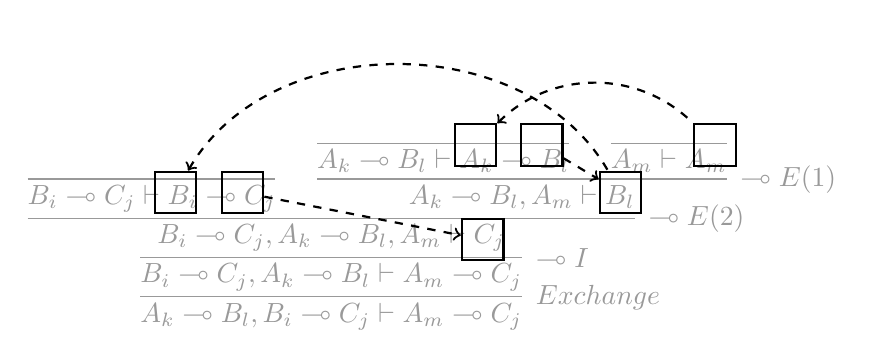
\begin{tikzpicture}[
		   focus/.style={rectangle, thick, draw, minimum size=15pt},
		   link/.style={thick, dashed}
	]
	\node[inner sep=0pt, outer sep=0pt] (bg) at (0,0) 
	{
	\textcolor{gray!80}{
	$
		\infer[\Exchange]{\nprop{A}_k\li\pprop{B}_l, \nprop{B}_i\li\pprop{C}_j \vdash \pprop{A}_m \li \nprop{C}_j}{
			\infer[\li I]{\nprop{B}_i\li\pprop{C}_j, \pprop{A}_k\li\pprop{B}_l \vdash  \pprop{A}_m \li \nprop{C}_j}{
				\infer[\li E (2)]{\nprop{B}_i\li\pprop{C}_j, \nprop{A}_k\li\pprop{B}_l, \pprop{A}_m \vdash \nprop{C}_j}{
					\infer[\Ax]{\nprop{B}_i\li\pprop{C}_j\vdash \pprop{B}_i \li \nprop{C}_j}{
					}
					&
					\infer[\li E (1)]{\nprop{A}_k\li\pprop{B}_l, \pprop{A}_m \vdash \nprop{B}_l}{
	  					\infer[\Ax]{\nprop{A}_k\li\pprop{B}_l \vdash \pprop{A}_k\li\nprop{B}_l}{	
						}
						&
						\infer[\Ax]{\pprop{A}_m \vdash \nprop{A}_m}{
						}
					}
				}
			}
		}
	$
	}
	};
	\node[focus] (ak) at (0.51, 1.125) {};
	\node[focus] (am) at (3.55,  1.125) {};
	\draw[link, <-] (ak) to[bend left=45] (am); %$(am.north)$);
	\node[focus] (bl1) at	(1.35, 1.125) {};
	\node[focus] (bl2) at (2.35, 0.525) {};
	\draw[link, ->] (bl1) -- (bl2);
	\node[focus] (bi) at (-3.3, 0.525) {};
	\node[focus] (cj1) at (-2.45, 0.525) {};
	\node[focus] (cj2) at (0.6, -0.075) {};	
	\draw[link, <-] (bi) to[bend left=60] (bl2);
	\draw[link, ->] (cj1) -- (cj2);
	\end{tikzpicture}
	\caption{Extracting axiom links from the proof of Figure~\ref{figure:funcomp}.}
	\label{figure:funcomp_annotated}
\end{figure}

Let's revisit the natural deduction proof of Figure~\ref{figure:funcomp}.
This time around, we will explicate polarity information, and put an identifying index to each atomic formula occurrence at its axiom leaves; 
the turnstile mirrors indices faithfully, but inverts atomic polarities.
Going bottom up through Figure~\ref{figure:funcomp_annotated}, every encounter of an implication elimination allows us (i) to identify the set of indices coming from the functor's negative part with the set of indices provided by the counterpart positive argument and (ii) to propagate the negative indices of the functor's remainder to the succedent of the next conclusion.
That is, the first elimination $\li E(1)$ creates the identification $\{k \leftrightarrow m\}$, and propagates the positive leftover $\nprop{B}_l$ to the next proof step, whereas the next elimination $\li E(2)$ identifies $\{i \leftrightarrow l\}$ and propagates $\nprop{C}_j$ downwards.
Upon reaching the proof's conclusion, we get to merge all identifications established along the proof%
\footnote{
Let's avoid any misteps here. The joining described is \textit{not} set-theoretic union. Rather, we first take the set-theoretic union, and then iteratively reduce the set by conflating all identifications that agree in at least one element, up to a fixpoint.
For instance, joining $\{ i \leftrightarrow k\}$ and $\{ l\leftrightarrow i, j \leftrightarrow m\}$ yields $\{i \leftrightarrow k \leftrightarrow l, j \leftrightarrow m \}$. Such a situation could arise for example when attempting to find the axiom links of non $\beta$ normal proofs, like
\[
\term{\left(\lam \Var{0}.\Var{0}^{\prop{a}_i \li \prop{b}_j}~\Var{1}^{\prop{a}_k}\right)~\Var{2}^{\prop{a}_l \li \prop{b}_m}}
\]
The added burden has the enormous benefit of yielding ``$\beta$ normalized'' links and resolving potential future headaches \textit{a priori}.
}%
, which can then be applied as a mapping (e.g. to the lexicographically first element) yielding a link-decorate judgement, in our case:
\[
	\nprop{a}_k \li \pprop{b}_i, \nprop{b}_i \li \pprop{c}_j \vdash \pprop{a}_k \li \nprop{c}_j
\]
Matching indices correspond exactly to the axiom links of Figure~\ref{subfigure:proof_structure_funcomp} -- the two representations are in fact equivalent.
Now, we really do know how to freely move back and forth between the proof net and natural deduction presentation of proofs in $\ILL_{\li}$.

The question then is: when should we use which?
The original intention of proof nets was to provide a compact, bureacracy-free representation of proofs that abstracts away from structural rules.
In that sense, their strength is also their weakness; same as the $\lam$-terms they prescribe, they encode the semantically essential part of a proof, but hide structural subtleties that can prove hard to guess or recover.
At the same time, performing search over proof nets is a horrible idea; the number of possible links we need to consider scales factorially with respect to the number of atoms in the proof frame, and checking whether a set of links is valid is in the best case linear.
Due to these limitations, proof nets were envisaged as a compiled form of an existing proof, rather than a canvas to find that proof on.
We will not see proof nets again for a while, but we will keep their memory warm in our hearts.
Because when we do, we will challenge this perception and see how their parallel nature can actually be very convenient for proof search.
Until then, we can temporarily store them in our mental backlog. 


\section{Lambek Calculi}\label{section:lambek_calculi}
\subsection{Dropping Commutativity}
There is only one structural rule left\footnote{Or is there?}: it is time for \Exchange{} to go.
Dropping \Exchange{} makes the structures of our logic non-commutative.
The transition, however, requires some care.
If we were to naively go about our business using the inherited $\ILL$ connectives, we would soon stumble upon a pitfall.
Recalling the shape of the $\li E$ rule, we come to the realization that functions carried over to this new logic are suddenly picky; they can only be applied to arguments to their right.
This should raise some flags: a directionally flavoured version of the implication is not bad in itself, but the presence of just such one such version is --  where shall we look for the left-biased one?
The answer is simple: the conflation between the two directions was natural, up until a moment ago; having them both would not amount to much, since by \Exchange{} they would be interderivable.
With \Exchange{} removed, the veil is lifted and we can now see this clearly: there were always two implications, except disguised by the same symbol!
Let us do our newfound friend justice, and make this distinction explicit.

The logic that provides us with the tools to accomplish this is due to Jim Lambek~\cite{lambek1958mathematics}, and has come to by known as the Lambek calculus $\LC$.
At this point, the careful reader will notice a chronological inconsistency in our presentational tour: the Lambek calculus predates Linear Logic! Despite the fact, it is in essence a \textit{refinement} of its purely linear part -- a substructural logic within a substructural logic -- and our previous exposition makes us better equiped to appreciate it.
With commutativity gone, the Lambek calculus brings \textit{order} to Linear Logic -- in the literal sense -- assumptions must now be used exactly in the order they were instantiated.
It also brings forth the notion of \textit{adjacency}: structures joined by a rule are now immobile, and therefore obliged to remain adjacent from then on, unless broken apart by abstractions.

Formulas in the Lambek calculus are generated by the grammar:
\begin{equation}
\prop{a}, \prop{b}, \prop{c} := p \ | \ \prop{a} \divleft \prop{b} \ | \ \prop{a} \divright \prop{b} \ | \ \prop{a} \otimes \prop{b}
% \ | \ \prop{a} \otimes \prop{b} \ | \ \prop{a} \with \prop{b}
\label{equation:LC}
\end{equation}
The rules of this fragment are presented in Figure~\ref{figure:lambek_calculus_rules}.
Alternative presentations can include additive conjunction and/or either of the disjunctions, but the key feature of interest lies in the two implications, $\divright$ and $\divleft$.
The intuitive way of reading those is as directed fractionals, the formula hidden under the cover of the slash being the divisor, and the formula lying on it the dividend.
The elimination rule $\divright E$ (resp. $\divleft E$) can then be read as fractional simplifications, whereby right (resp. left) multiplication by the divisor cancels out the division as a whole.
An analogus reading can be attributed to the introduction rules, them now being the instantiation of a division by withdrawing items from the left or right of the assumption sequence (it might be helpful to think of $\divright I$ as dequeuing and $\divleft I$ as popping from the assumptions in the premise).
The division paradigm is of pedagogical utility only, and we will not take it any further for fear of (incorrectly) hinting at other properties of fractionals being applicable in the logic.
A noteworthy change of notation appears in the elimination of the product: with $\Delta\ctx{\Gamma}$ we denote a structure $\Delta$ containing substructure $\Gamma$: $\Delta\ctx{\_}$ now serves as a \textit{context}, i.e. a structure of assumptions with a hole.
The rule now claims it is acceptable to \textit{replace} substructure $\smallprop{A}, \smallprop{B}$ in $\Delta$ by $\Gamma$, if $\Gamma \vdash \smallprop{A}\otimes\smallprop{B}$ holds.
The notions of structure and substructure depend of course on the logic used -- in the current setting, $\Delta$ is a sequence, to which $\Gamma$ is a subsequence. 
The reformulation of the rule is necessary to arbitrate elimination of nested products, since their extraction to the right or left edge of an assumption sequence is no longer possible.
This also serves to better illustrate a remark made earlier: the rule can be applied at arbitrary nesting depths, each position corresponding to a supposedly different proof (consider for instance that if $\Delta\ctx{\Gamma}$, and $\Gamma\ctx{\smallprop{A}, \smallprop{B}}$, then it is also the case that $\Delta\ctx{\prop{a}, \prop{b}}$).

\begin{figure}
	\centering
	\begin{tabularx}{0.975\textwidth}{@{}CC@{}}
		\multicolumn{2}{@{}c@{}}{$\infer[\Ax]{\term{\vari }: \prop{a} \vdash \term{\vari }: \prop{a}}{}$}\\[2em]
		$\infer[\divright E]{\Gamma, \Delta \vdash \term{s}\appright\term{t}: \prop{b}}{\Gamma \vdash  \term{s}: \prop{b} \divright \prop{a} & \Delta \vdash \term{t}: \prop{a}}$
		& 
		$\infer[\divright I]{\Gamma \vdash \term{\lam \vari .s}: \prop{b} \divright \prop{a}}{\Gamma, \term{\vari }: \prop{a} \vdash \term{s}: \prop{b}}$\\[2em]
		$\infer[\divleft E]{\Gamma, \Delta \vdash \term{s}\appleft\term{t}:\prop{b}}{\Gamma \vdash \term{s}:\prop{a} & \Delta \vdash \term{t}:\prop{a}\divleft\prop{b}}$
		& 
		$\infer[\divleft I]{\Gamma \vdash \term{\adbmal \vari .s}: \prop{a} \divleft \prop{b}}{\term{\vari }: \prop{a}, \Gamma \vdash \term{s}: \prop{b}}$\\[2em]
		$\infer[\otimes E]{\Delta\ctx{\Gamma} \vdash \cterm{case \term{s} of \term{(\vari , \varj)} in \term{t}}: \prop C}{
			\Gamma \vdash \term{s}: \prop{a}\otimes\prop{b}
			&
			\Delta\ctx{\term{\vari }: \prop{a}, \term{\varj}: \prop{b}}  \vdash \term{t}: \prop C}$
		&
		$\infer[\otimes I]{\Gamma,\Delta \vdash \term{(s,t)}: \prop{a} \otimes \prop{b}}{\Gamma \vdash \term{s}: \prop{a} & \Delta \vdash \term{t}: \prop{b}}$\\[2em]
	\end{tabularx}
	\caption{Lambek calculus $\LC$.}
	\label{figure:lambek_calculus_rules}
\end{figure}

The Lambek calculus hails from an intuitionistic tradition, and is thus amenable to a propositions as types interpretation~\cite{wansing1990formulas}.
Addorning its rules with faithful term rewrites translates into a type system that is both linear and ordered~\cite{pierce2004advanced}.
Things get funky there: we now have two distinct modes of function application and $\lam$ abstraction, each pair with its own reduction.
We use $\appright$ and $\appleft$ to denote right and left application, respectively -- the mnemonic is that the triangle points to the function -- and $\lam$ and $\adbmal$ to denote the two kinds of anonymous functions.

\subsubsection{Proof \& Term Reductions}
The proof reductions of Figure~\ref{figure:lambek_proof_reductions} should be at this point straightforward to decode.
The only addition is the symmetric version of the familiar implicational redex.
For the redex of the product, the substituted $\smallprop{A}$ and $\smallprop{B}$ hypotheses are now wrapped on both sides by a context $\Theta$, following the formulation of $\otimes E$.
The corresponding term reductions are:
\begin{align}
(\term{\lam \vari .s})\appright\term{t} & \bred \term{s}_{[\term{\vari } \mapsto \term{t}]}\\
\term{t}\appleft(\term{\adbmal \vari .s}) & \bred \term{s}_{[\term{\vari } \mapsto \term{t}]}\\
\cterm{case (\smallterm{s}, \smallterm{t}) of (\smallterm{\vari }, \smallterm{\varj}) in \smallterm{u}} & \bred \term{u_{[\term{s} \mapsto \term{\vari }, \term{t} \mapsto \term{\varj}]}}
\end{align}

\begin{figure}
	\centering
	\begin{tabularx}{0.95\textwidth}{@{}ccc@{}}
	$\infer[\divright E]{\Gamma, \Delta \vdash \prop{b}}{
	\infer[\divright I]{\Gamma \vdash \prop{b} \divright \prop{a}}{
		\infer*[s]{\Gamma, \prop{a} \vdash \prop{b}}{
				\infer[\Ax]{\prop{a} \vdash \prop{a}}{} 
			}
		}
		&
		\infer{\Delta \vdash \prop{a}}{
			\infer*[t]{}{}
		}
	}$
	&
	\raisebox{20pt}{$\implies$}
	&
	$ 
	\infer[]{\Gamma, \Delta \vdash \prop{b}}{
		\infer*[s]{}{
		\infer[]{\Delta \vdash \prop{a}}{
			\infer*[t]{}{}
		}}
	}
	$\\[\smallsep]
	$\infer[\divleft E]{\Gamma, \Delta \vdash \prop{b}}{
		\infer{\Gamma \vdash \prop{a}}{
			\infer*[t]{}{}
		}
		&
		\infer[\divleft I]{\Delta \vdash \prop{a} \divleft \prop{b}}{
			\infer*[s]{\prop{a}, \Delta \vdash \prop{b}}{
				\infer[\Ax]{\prop{a} \vdash \prop{a}}{} 
			}
		}
	}$
	&
	\raisebox{20pt}{$\implies$}
	&
	$ 
	\infer[]{\Gamma, \Delta \vdash \prop{b}}{
		\infer*[s]{}{
		\infer[]{\Gamma \vdash \prop{a}}{
			\infer*[t]{}{}
		}}
	}
	$\\[\smallsep]
	$
	\infer[\otimes E]{\Theta\ctx{\Gamma, \Delta} \vdash \prop{c}}{
		\infer[\otimes I]{\Gamma, \Delta \vdash \prop{a} \otimes \prop{b}}{
			\infer[]{\Gamma \vdash \prop{a}}{\infer*[s]{}{}}
			&
			\infer[]{\Delta \vdash \prop{b}}{\infer*[t]{}{}}
		}		
		&
		\infer*[u]{\Theta\ctx{\prop{a}, \prop{b}} \vdash \prop{c}}{
			\infer[\Ax]{\prop{a} \vdash \prop{a}}{}
			& 
			\infer[\Ax]{\prop{b} \vdash \prop{b}}{}
		}
	}
	$
	&
	\raisebox{20pt}{$\implies$}
	&
	$
	\infer*[u]{\Theta\ctx{\Gamma, \Delta} \vdash \prop{c}}{
		\infer[]{\Gamma \vdash \prop{a}}{
			\infer*[s]{}{}
		}
		&
		\infer[]{\Delta \vdash \prop{b}}{
			\infer*[t]{}{}
		}
	}
	$
	\end{tabularx}
	\caption{Lambek $\beta$ redexes.}
	\label{figure:lambek_proof_reductions}
\end{figure}

\subsection{Dropping Associativity}
Judging by the apparent absence of any more structural rules to remove, someone eager to be done with the whole story could at this point proclaim our substructural tour finished.
We are not quite done yet, however, for one last structural equivalence still remains unchecked (one we have made extensive use of, for that matter).
The culprit can be found by going back to our original definition of structures in the long and distant past of Subsection~\ref{subsection:intuitionistic_logic} -- by treating them as sequences, we have mindlessly equipped them with \textit{associativity} for free, the use of which we never made explicit.
The one to notice was Lambek once more~\cite{lambek1961calculus}.
In the new logic (pragmatically named the non-associative Lambek calculus $\NL$) the definition of a structure changes to:
\begin{equation}
	\Gamma, \Delta, \Theta := \ \prop{a} \ | \ (\Gamma \sbind \Delta)
\end{equation}
i.e. the structural unit of the empty sequence is no more, and the scope of the binary structural binder is made explicit with brackets (we use the distinct symbol \sbind{} to tell this new structural binder apart from its associative sibling).
On top of adjacency and order, the non-associative Lambek calculus further considers \textit{constituency}; structures are now binary trees, with atomic propositions as their leaves and \sbind{} as branching nodes, and judgements are differentiated on the basis of the binary branching form their assumptions take.
Formulas remain as they were, but the presentation of the rules changes to that of Figure~\ref{figure:non_assoc_lambek_rules} in order to accommodate the new, stricter structures.
Merging structures $\Gamma$ and $\Delta$ via $\divleft E$, $\divright E$ or $\otimes I$ is translated to building up a tree with the two as branches.
Decomposing a structure via an abstraction $\divleft I$ or $\divright I$ now requires that the formula abstracted over occurs not just at the edge of the tree's linear projection, but also at its top-most branching level.
The notation $\Gamma\ctx{\Delta}$ now denotes that $\Delta$ is a \textit{subtree} of $\Gamma$ -- for the product elimination $\otimes E$ to be applicable, $\prop{a}$ and $\prop{b}$ need not just be adjacent, but also commonly rooted.

\begin{figure}
	\centering
	\begin{tabularx}{0.99\textwidth}{@{}CC@{}}
		\multicolumn{2}{@{}c@{}}{$\infer[\Ax]{\term{\vari }: \prop{a} \vdash \term{\vari }: \prop{a}}{}$}\\[2em]
		$\infer[\divright E]{(\Gamma \sbind \Delta) \vdash \term{s}\nappright\term{t}: \prop{b}}{\Gamma \vdash \term{s}: \prop{b} \divright \prop{a} & \Delta \vdash \term{t}: \prop{a}}$
		& 
		$\infer[\divright I]{\Gamma \vdash \term{\lam \vari .s}: \prop{b} \divright \prop{a}}{(\Gamma \sbind \term{\vari }: \prop{a}) \vdash \term{s}:\prop{b}}$\\[2em]
		$\infer[\divleft E]{(\Gamma \sbind \Delta) \vdash \term{s}\nappleft\term{t}:\prop{b}}{\Gamma \vdash \term{s}: \prop{a} & \Delta \vdash \term{t}: \prop{a}\divleft\prop{b}}$
		& 
		$\infer[\divleft I]{\Gamma \vdash \term{\adbmal \vari .s}: \prop{a} \divleft \prop{b}}{(\term{\vari }: \prop{a} \sbind \Gamma) \vdash  \term{s}:\prop{b}}$\\[2em]
		$\infer[\otimes E]{\Delta\ctx{\Gamma} \vdash \cterm{case \term{s} of \term{(\vari , \varj)} in \term{t}}: \prop C}{
			\Gamma \vdash \term{s}: \prop{a}\otimes\prop{b}
			&
			\Delta\ctx{(\term{\vari }: \prop{a}, \term{\varj}: \prop{b})}  \vdash \term{t}: \prop C}$
		&
		$\infer[\otimes I]{\Gamma,\Delta \vdash \term{(s,t)}: \prop{a} \otimes \prop{b}}{\Gamma \vdash \term{s}: \prop{a} & \Delta \vdash \term{t}: \prop{b}}$
	\end{tabularx}
	\caption{Non-associative Lambek calculus $\NL$.}
	\label{figure:non_assoc_lambek_rules}
\end{figure}

The syntax of the isomorphic $\lam$-calculus is identical to before, except this time we use $\nappright$ and $\nappleft$ to notationally differentiate with the non-associative application (not unlike how we replaced the intuitionistic implication $\ii$ with its linear counterpart $\li$ earlier).
The new structural constraint on the introduction of a directed implication can be intuititively translated to a constraint on the applicability of an abstraction.
Namely, the variable to abstract over needs to occur at the top-most level of a function application in the term's inductive body.%
\footnote{Abusing terminology, here by inductive body we mean the term itself (if it's an implicative one), the term's inner body (if it's a sequence of abstractions), the left or right coordinate (if it's a product), or the nested body on which substitution is performed (if it's a deconstructed product).}

\subsubsection{Proof \& Term Reductions}
Proof \& term reductions are notationally identical to those of the previous subsection, modulo bracketing, and substituting white for black triangles.
I trust the missing picture is easy enough to create mentally.


\subsection{The Full Landscape}
We have seen $\NL$ as a refinement of $\LC$, and $\LC$, in turn, as a refinement of $\ILL$.
The three can be perceived as points in a lattice of substructural logics, upon which we can move by adding or removing structural rules at a global level; this view lends $\ILL$ its alternative name $\LP$, for the Lambek calculus with permutation (also encountered as the Lambek-van Benthem Calculus~\cite{van1988semantics}).
At the top of the diamond we have $\ILL$, where (linearity aside), anything goes, and at the bottom we have $\NL$, where neither associativity nor commutativity hold.
At the center, there's $\LC$, where only associativity holds.
Next to it, an unexpected curiosity pops up: $\NLP$ (for the non-associative Lambek with permutation), an offbeat logic where associativity holds but commutativity doesn't -- its structures are \textit{mobiles}: orderless, binary branching trees that make no distinction between left and right daughters.
Unlike its relatives, $\NLP$ has received limited attention from theorists and practitioners alike.
This will still remain the case even after (if?) this manuscript sees the light of day, but its peculiar structures will reemerge and have their moment to shine  later on.

\begin{figure}
	\centering
	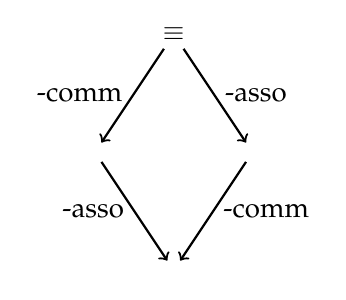
\begin{tikzpicture}[g/.style={outer sep=3pt, inner sep=0pt,minimum width=4pt},e/.style={thick,->}]
		\node[g] (ILL) at (0,0)			{$\LP \equiv \ILL$};
		\node[g] (LC)	at (-1, -1.5)		{$\LC$};
		\node[g] (NL)	at (0, -3)		{$\NL$};
		\node[g] (NLP) at (1, -1.5)		{$\NLP$};
		
		\draw[e] (ILL) -- (LC) node[midway,left]{-comm};
		\draw[e] (LC) -- (NL) node[midway,left]{-asso};
		\draw[e] (ILL) -- (NLP) node[midway,right]{-asso};
		\draw[e] (NLP) -- (NL) node[midway,right]{-comm};
		\
	\end{tikzpicture}
	\label{figure:substructural_logics}
	\caption{$\logic{(N)L(P)}$: $\ILL$ and substructural friends.}
\end{figure}


%\paragraph{Proof nets}
%\todo{}

\section{Restoring Control}\label{section:modalities}
With every step we have taken further into substructuraland, we have been paying a price in expressivity; it is now time for us to acknowledge the accumulated bill.
Dropping \Contraction{} and \Weakening{} made us resource conscious, but theorems of $\IL$ that required resource duplication or erasure became underivable.
Dropping \Exchange{} forced us to pay attention to the order of assumptions, but costed us access to theorems that required permutation to derive.
Substituting the structural comma $\_,\_$ with the non-associative $(\_\sbind\_)$ casted our sequences to trees, this time at the expense of theorems that required rebracketing.
Woe is us -- is there even anything left we can derive?

Perhaps this is painting an overly dramatic picture, considering that none of this is necessarily bad.
From an epistemic perspective, the less structural equivalences we take for granted, the better our mental grasp of structural difference becomes.
In the best case, if it just so happens that the kind of structures we want to investigate overlaps \textit{fully} with the kind of structures our logic can explicitly reason about, the distinction between theorem and non-theorem becomes a refinement rather than a loss of expressivity.
From a more pragmatic perspective, more structural constraints means easier proof search, and less theorems means faster exhaustion of possibilities.
To make the scale of the combinatorics tangible, reflect for a second on this.
A single judgement of $n$ hypotheses in $\NL$ is but one of the Catalan number of bracketings $C(n)$ it would be syntactically undistinguishable from in $\LC$, each one of which in turn is but one of the factorially many permutations $n!$ it would be equivalent to in $\LP$.%
\footnote{Boom, goes the combinatorial explosion.}
In the case for checking the satisfiability of a judgement (i.e. searching for \textit{any} valid proof), all the above would have made for potential proof candidates;
in the case for attempting to enumerate the proofs of a judgement (i.e. searching for \textit{all} valid proof), they would all have needed to be exhausted.
The point to take home is that proof search becomes decidedly easier in the absence of syntactic equivalences, so perhaps a double-edged sword would have made for a better analogy than a bill.

The defeatist attitude here would be to just accept the trade-off between expressivity and complexity, weep for the theorems forever lost, take our victory and walk away.
The problem lies however in the common occasion where the structure of objects under scrutiny overlaps only \textit{partially} with a specific substructural flavour, modulo some exceptional but real cases that require added expressivity.
In such a scenario, taking a step up in the hierarchy would cause an undesirable combinatorial explosion, whereas staying put would sacrifice our ability to argue about these exceptional cases. 
By contrast, the maximalist attitude makes no concessions and seeks both for the cake to be whole and the dog to be fed.%
\footnote{Direct translation of a silly but fitting Greek aphorism that won by a small margin over the Italian equivalent (wine barrel full and wife drunk). In any case, cake is bad for dogs.}
What if there was a way to keep our logic computationally tractable but with temporary and on-demand access to normally excluded reasoning tools?

\subsection{The Logic of Modalities}\label{subsec:modal_logic}
The answer comes in the form of unary \textit{modalities}, type-forming operators lent from modal logics, that allow navigation between logics of different structural properties.
Unary modalities hold a key role in the presentation of full linear logic; there, a single operator $!$ (called \textit{bang}) would allow an embedding of intuitionistic (non-linear) propositions into the linear regime, essentially acting as a licensor of \Contraction{} and \Weakening{}.
In our case, we will make do with two modalities from temporal logic, the diamond $\diamond$ and the box $\Box$.

The two form a residuated pair, the properties of which can be formulated either (i) in the form of a type-level biconditional derivability relation:
\begin{equation}
		\diamond \prop{a} \vdash \prop{b}\text{ iff }\prop{a} \vdash \Box\prop{b}
\end{equation}
or (ii) the monotonic behavior of its parts:
\begin{align}
		\prop{a} \vdash \prop{b} & \implies \diamond \prop{a}\vdash \diamond\prop{b}\\
		\prop{a} \vdash \prop{b} & \implies \Box{\prop{a}}\vdash \Box\prop{b}
\end{align}
and the adjointness of their compositions, where $\diamond\Box(\_)$ is an \textit{interior} and $\Box\diamond(\_)$ a \textit{closure} operator:
\begin{align}
		\Gamma \vdash \prop{a} 				& \implies \Gamma \vdash \Box\diamond\prop{a} \label{equation:closure}\\
		\Gamma \vdash \diamond\Box\prop{a} & \implies \Gamma \vdash \prop{a} \label{equation:interior}
\end{align}

\begin{figure}
	\centering
	\begin{tabularx}{0.9875\textwidth}{@{}CC@{}}
		$\infer[\Box E]{\bracket{\Gamma} \vdash \boxelim{\term{s}}: \prop{a}}{
			\Gamma \vdash \term{s}: \Box\prop{a}
		}$
		&
		$\infer[\Box I]{\Gamma \vdash \boxintro{\term{s}}:\Box\prop{a}}{
			\bracket{\Gamma} \vdash \term{s}:\prop{a}
		}$
		\\[\smallsep]
		$\infer[\diamond E]{\Gamma\ctx{\Delta} \vdash \cterm{case \term{\diaelim t} of \term{\vari } in \term{s}}: \prop{b}}{
			\Gamma\ctx{\bracket{\term{\vari }:\prop{a}}}\vdash\term{s}:\prop{b}
			&
			\Delta \vdash \term{t}:\diamond\prop{a}
		}
		$
		&
		$\infer[\diamond I]{\bracket{\Gamma} \vdash \diaintro{\term{s}}: \diamond \prop{a}}{
			\Gamma \vdash \term{s}:\prop{a}
		}$
	\end{tabularx}
	\caption{Logical rules of modal inference.}
	\label{figure:modal_logical}
\end{figure}

The logical manipulation of these modalities is handled by corresponding elimination and introduction rules, presented in Figure~\ref{figure:modal_logical}.
The presentation is intentionally detached from a specific subtructural strand -- modalities are plug-and-play to any member of the $\logic{(N)L(P)}$ family.
Their incorporation adds a new kind of structure to the ones provided by the underlying logic, altering judgements accordingly:
\begin{equation}
	\Gamma, \Delta, \Theta := \dots \ | \ \bracket{\Gamma}
\end{equation}

Angular brackets denote unary tree branches that behave slightly different to the rest; they act as an impenetrable barrier that permits or hinders the introduction or elimination of modal connectives in a judgement.
The box elimination rule $\Box E$ grants us the option of removing a logical box from the succedent of the premise (as long as it is its main connective), but encloses the premises in angular brackets in the process.
Its introduction counterpart $\Box I$ does the exact opposite: it frees a judgement's assumptions from their brackets, but puts the succedent proposition under the scope of a box.
The diamond behaves just the other way around.
Its introduction rule $\diamond I$ is straightforward: it offers the possibility of putting the succedent under the scope of a diamond, in exchange wrapping the antecedents with brackets.
The elimination rule $\diamond E$ is more of a problem child, behaving akin to a unary product.
Without locality restrictions, it inspects a proof of $\smallprop{B}$, the assumptions of which contain a substructure $\bracket{\smallprop{A}}$ within context $\Gamma{\ctx{\_}}$, and allows the post-hoc substitution of the hypothesis together with its brackets by a structure $\Delta$, if from it one can derive $\diamond \smallprop{A}$.

Rules are adorned with term rewrite instructions in the propositions as types style, similar to how temporal logic can be operationalized in the $\lam$-calculus~\cite{wansing2002sequent}.
The mnemonic is now two-dimensional: upward triangles denote introduction and downward ones elimination, whereas black triangles are for the box, white ones for the diamond.
Term constructions for the single-premise rules are uncomplicated: each type operation just leaves the corresponding term footprint.
This is not the case for the $\diamond E$ rule, which requires some attention:
the structural substitution of $\bracket{\smallprop{A}}$ for $\Delta$ necessitates a case construct that calls for a term substitution of the variable $\smallterm{\vari }$ for $\diaelim\smallterm{t}$.
Note that the free variables of the resulting expression ($\caseof{\diaelim t}{\vari }{s}$) are the union of the free variables of \smallterm{t} and those of \smallterm{s} except for \smallterm{\vari }, which becomes \textit{bound} by the case construct.

\subsubsection{Proof \& Term Reductions}
\begin{figure}
	\begin{subfigure}{1\textwidth}
	\centering
		\begin{tabularx}{0.85\textwidth}{@{}ccc@{}}
		$\infer[\Box E]{\bracket{\Gamma} \vdash \prop{a}}{
			\infer[\Box I]{\Gamma \vdash \Box \prop{a}}{
				\infer*[s]{\bracket{\Gamma} \vdash  \prop{a}}{}
			}
		}
		$
		&
		\raisebox{10pt}{$\implies$}
		&
		$\infer*[s]{\bracket{\Gamma} \vdash \prop{a}}{}
		$\\[\smallsep]
		$\infer[\diamond E]{\Gamma\ctx{\bracket{\Delta}} \vdash \prop{b}}{
			\infer*[s]{\Gamma\ctx{\bracket{\prop{a}}} \vdash \prop{b}}{
				\infer[\Ax]{\prop{a} \vdash \prop{a}}{}}
			&
			\infer[\diamond I]{\bracket{\Delta} \vdash \diamond\prop{a}}{
				\infer*[t]{\Delta \vdash \prop{a}}{}
			}
		}
		$
		&
		\raisebox{20pt}{$\implies$}
		&
		$\infer*[s]{\Gamma\ctx{\bracket{\Delta}} \vdash \prop{b}}{
			\infer*[t]{\Delta \vdash \prop{a}}{}
		}
		$
		\end{tabularx}
		\caption{Modal $\beta$ redexes.}
		\label{subfigure:modal_beta_reductions}
	\end{subfigure}\\[\midsep]
	\begin{subfigure}{1\textwidth}
	\centering
		\begin{tabularx}{0.8\textwidth}{@{}ccc@{}}
			$\infer[\Box I]{\Gamma \vdash \Box\prop{a}}{
			\infer[\Box E]{\bracket{\Gamma} \vdash \prop{a}}{
					\infer*[s]{\Gamma \vdash  \Box\prop{a}}{}
				}
			}
			$
			&
			\raisebox{5pt}{$\equiv$}
			&
			$\infer*[s]{\Gamma \vdash \Box\prop{a}}{}
			$\\[\smallsep]
			$\infer[\diamond E]{\Delta \vdash \diamond\prop{a}}{
				\infer[\diamond I]{\bracket{\prop{a}}\vdash \diamond \prop{a}}{
					\infer[\Ax]{\prop{a} \vdash \prop{a}}{}
				}
				&
				\infer*[s]{\Delta \vdash \diamond\prop{a}}{}
			}$
			&
			\raisebox{15pt}{$\equiv$}
			&
			$\infer*[s]{\Delta \vdash \diamond \prop{a}}{}
			$
		\end{tabularx}
	\caption{Modal $\eta$ redexes.}
	\label{subfigure:modal_eta_reductions}
	\end{subfigure}
	\caption{Modal redexes}
	\label{figure:modal_reductions}
\end{figure}

The proof patterns of Figure~\ref{subfigure:modal_beta_reductions} exhibit introduction elimination chains of modal operators, and thus constitute $\beta$ redexes subject to normalization.
The first one is trivial: it just says that a sequential application of $\Box I$ followed by $\Box E$ can be safely excised.
The second one proposes that if a $\diamond I$ is the last rule to have been applied on the substitution branch $t$ of the $\diamond E$ rule, it would make sense to simply plug proof $t$ in place of the proposition $\smallprop{A}$ hypothesized in the other  branch $s$.
On the term level, these rules correspond to computations:
\begin{align}
\boxelim \boxintro \term{s} & \bred \term{s}\\
\cterm{case \term{\diaelim \diaintro t} of \term{x} in \term{s}} & \bred \term{s}_{[\term{x} \mapsto \term{t}]}
\end{align}

The dual direction of $\eta$ equivalences also holds -- since these are discovered in the literature less frequently than the more pedestrian implication and product equivalences, we explictly present them in Figure~\ref{subfigure:modal_eta_reductions}.
The term equivalences they materialize are:
\begin{align}
\boxintro \boxelim \term{s} & \overset{\eta}{\equiv} \term{s}\\
\cterm{case \term{\diaelim{s}} of \term{x} in \term{\diaintro{x}}} & \overset{\eta}{\equiv} \term{s}
%\cterm{case \term{\diaelim \diaintro t} of \term{x} in \term{s}} & \bred \term{s}_{[\termt{x} \mapsto \term{t}]}
\end{align}

\subsubsection{A Digression on Modal Terms}
For the modally savvy, the term rewrites attributed to the modal rules might seem unorthodox.
A more common presentation employs the simpler meta-syntax notation of term substitution.
For instance, $\diamond E$ can often be spotted in the wild as:
\[
	\infer[\diamond E]{\Gamma\ctx{\Delta} \vdash \term{s}_{[\term{\vari }\mapsto\term{\diaelim t}]}: \prop{b}}{
		\Gamma\ctx{\bracket{\term{\vari }:\prop{a}}}\vdash\term{s}:\prop{b}
		&
		\Delta \vdash \term{t}:\diamond\prop{a}
	}
\]
In this disguise, the rule is again seen as realizing a retroactive substitution of $\smallterm{\vari }$ with $\smallterm{\diaelim t}$, except this time around the substitution is \textit{actually} performed, resulting in less cumbersome terms being carried around.

Opting for this alternative notation has, however, a number of negative consequences.
The more superficial one is that the main term connective does not take scope at the outermost layer of rule's yield, but rather nested arbitrarily deeply within it, unlike its better behaved version.
From a proof-theoretic perspective, normalization is now baked directly into the theory, as the term yield of the rule exactly coincides with its $\beta$ reduced form.
At the same time, all rule permutations boil down to having the exact same reduction, i.e. multiple previously distinct terms are conflated into a single representation.
This establishes an impicit syntactic equivalence on proofs that claims that the exact position of the $\diamond E$ rule is \textit{syntactically irrelevant} (so long of course as the same variable $\smallterm{\vari }$ is substituted by the same term $\smallterm{\diaelim t}$).
Finally, the shorthand version hides variables; hypotheses that would be bound by the case construct are instead erased and forgotten, obfuscating the term-to-proof correspondence.
All these are perhaps minor points not worth taking too seriously, but for one concerned with concrete implementation the extra merit of notational simplicity comes at the cost of equality checking become way more tedious.
With this in mind (and in a rare moment of excessive formal zeal), we will exercise some self restraint and avoid indulging in the convenience of this version.

\subsubsection{Properties}

\begin{figure}
	\centering
	\begin{subfigure}{1\textwidth}
		\[
			\infer[\diamond E]{\term{\varj}: \diamond \prop{a} \vdash  \cterm{case \term{\diaelim \varj} of \term{\vari } in \term{s}}: \diamond \prop{b}}{
					\infer[\diamond I]{\bracket{\term{\vari }: \prop{a}} \vdash \diaintro \term{s}: \diamond \prop{b}}{
						\infer*[s]{\term{\vari }: \prop{a} \vdash \term{s}: \prop{b}}{}
					}
					&
					\infer[\Ax]{\term{\varj}: \diamond \prop{a} \vdash \term{\varj}: \diamond \prop{a}}{}
			}
		\]
		\caption{Monotonicity of the diamond.}
		\label{subfigure:modal_properties:diamond_mono}
	\end{subfigure}\\[\midsep]
	\begin{subfigure}{1\textwidth}
		\[
			\infer[\Box I]{\term{\varj}: \Box \prop{a} \vdash \boxintro{(\term{\lam \vari .s})~\term{\boxelim \varj}}:\Box \prop{b}}{
				\infer[\li E]{\bracket{\term{\varj}: \Box \prop{a}} \vdash (\term{\lam \vari .s})~\term{\boxelim \varj}: \prop{b}}{
					\infer[\li I]{\vdash \term{\lam \vari .s}: \prop{a} \li\prop{b}}{
						\infer*[s]{\term{\vari }: \prop{a} \vdash \term{s}: \prop{b}}{}
					}
					&
					\infer[\Box E]{\bracket{\term{\varj}: \Box \prop{a}} \vdash \boxelim\term{\varj}:\prop{a}}{	
						\infer[\Ax]{\term{\varj}: \Box\prop{a} \vdash \term{\varj}: \Box\prop{a}}{}
					}
				}
			}
		\]
		\caption{Monotonicity of the box.}
		\label{subfigure:modal_properties:box_mono}
	\end{subfigure}\\[\midsep]
	\begin{subfigure}{0.4\textwidth}
		\[
		\infer[\Box I]{\Gamma \vdash \boxintro\diaintro\term{s}:\Box \diamond \prop{a}}{
			\infer[\diamond I]{\bracket{\Gamma} \vdash \diaintro\term{s}: \diamond \prop{a}}{
				\infer*[s]{\Gamma \vdash \term{s}: \prop{a}}{}
			}
		}
		\]
		\caption{The closure $\diamond\Box(\_)$.}
		\label{subfigure:modal_properties:closure}
	\end{subfigure}%
	\begin{subfigure}{0.5\textwidth}
		\[
		\infer[\diamond E]{\Gamma \vdash \cterm{case \term{\diaelim{s}} of \term{\vari } in \term{\boxelim \vari }}: \prop{a}}{
						\infer[\Box E]{\bracket{\term{\vari }: \Box \prop{a}}\vdash \boxelim\term{\vari }:\prop{a}}{
							\infer[\Ax]{\term{\vari }: \Box\prop{a} \vdash \term{\vari }: \Box\prop{a}}{}
						}
						&
						\infer*[s]{\Gamma\vdash \term{s}: \diamond \Box \prop{a}}{}
				}
		\]
		\caption{And the interior $\Box\diamond(\_)$.}
		\label{subfigure:modal_properties:interior}
	\end{subfigure}\\[\midsep]
	\begin{subfigure}{1\textwidth}
		\[
			\infer[\diamond E]{\term{\varj}: \diamond \prop{a} \vdash \caseof{\diaelim \varj}{\vari }{s}:\prop{b}}{
				\infer[\Box E]{\bracket{\term{\vari }: \prop{a}} \vdash \boxelim\term{s}: \prop{b}}{
					\infer*[s]{\term{\vari }: \prop{a} \vdash \term{s}: \Box\prop{b}}{}
				}
				&
				\infer[\Ax]{\term{\varj}: \diamond \prop{a} \vdash \term{\varj}: \diamond \prop{a}}{}
			}
		\]
	\caption{Residuation law: from $\smallprop{A} \vdash \Box\smallprop{B}$ to $\diamond\smallprop{A} \vdash \smallprop{B}$.}
	\label{subfigure:modal_properties:residuation:1}	
	\end{subfigure}\\[\midsep]
	\begin{subfigure}{1\textwidth}
		\[
			\infer[\Box I]{\term{\varj}: \diamond \prop{a} \vdash \boxintro(\caseof{\diaelim \diaintro \varj}{\vari }{\lam \vari .s}): \prop{b}}{
				\infer[\diamond E]{\bracket{\term{\varj}: \prop{a}} \vdash \caseof{\diaelim \diaintro \varj}{\vari }{\lam \vari .s}: \prop{b}}{
					\infer[\li I]{\vdash \term{\lam \vari .s}: \diamond\prop{a} \li \prop{b}}{
						\infer*[s]{\term{\vari }: \diamond\prop{a} \vdash \term{s}: \prop{b}}{}
					}
					&
					\infer[\diamond I]{\bracket{\term{\varj}: \prop{a}} \vdash \term{\diaintro \varj}: \diamond \prop{a}}{
						\infer[\Ax]{\term{\varj}: \prop{a} \vdash \term{\varj}: \prop{a}}{}
					}
				}
			}
		\]
		\caption{Ditto, the other way around.}
		\label{subfigure:modal_properties:residuation:2}	
	\end{subfigure}
	\caption{Derivations for the various aspects of residuation.}
	\label{figure:modal_properties:residuation}
\end{figure}

Situating our unary operators within the modal logic zoo is no trivial endeavour (especially if you, like me, have had limited exposure to it before).
They are best characterized by the properties they satisfy, so inspecting them should shed some light on their proof-theoretic behavior (as a bonus, it will also help us get better acquainted with the kind of term rewrites their rules prescribe).
Figure~\ref{figure:modal_properties:residuation} presents the proof transformations equivalent to the properties foretold:
 (\subref{subfigure:modal_properties:diamond_mono}) and (\subref{subfigure:modal_properties:box_mono}) for monotonicity, (\subref{subfigure:modal_properties:closure}) and (\subref{subfigure:modal_properties:interior}) for composition, and (\subref{subfigure:modal_properties:residuation:1}) and (\subref{subfigure:modal_properties:residuation:2}) for the two directions of the residuation law.
 
Worth a special mention are also the so-called triple laws:
\begin{align}
	\diamond\prop{a} \dashv\vdash \diamond\Box\diamond\prop{a}\\
	\Box\prop{a} \dashv\vdash \Box\diamond\Box\prop{a}
\end{align}
which can be intuitively read as claiming that prepending an already modal type with (one or more) diamond-box pairs in alteration has no real effect, as these can unconditionally cancel out or be expanded into.
Figure~\ref{figure:modal_triple_laws} presents proofs of the above in both directions.


\begin{figure}
	\centering
	\begin{subfigure}{1\textwidth}
		\[
			\infer[\Box I]{\term{\varj}: \Box\diamond\Box\prop{a} \vdash \boxintro(\caseof{\diaelim \boxelim \varj}{\vari }{\boxelim{\vari }}): \Box\prop{a}}{
				\infer[\diamond E]{\bracket{\term{\varj}: \Box\diamond \prop{a}} \vdash \caseof{\diaelim \boxelim \varj}{\vari }{\boxelim{\vari }}: \prop{a}}{
					\infer[\Box E]{\bracket{\term{\vari }: \Box \prop{a}} \vdash \term{\boxelim \vari }:\prop{a}}{
						\infer[\Ax]{\term{\vari }: \Box\prop{a} \vdash \term{\vari }: \Box\prop{a}}{}
					}
					&
					\infer[\Box E]{\bracket{\term{\varj}:\Box\diamond\Box\prop{a}} \vdash \term{\boxelim \varj}:\diamond\Box\prop{a}}{
						\infer[\Ax]{\term{\varj}: \Box\diamond\Box\prop{a}\vdash\term{\varj}:\Box\diamond\Box\prop{a}}{}
					}
				}
			}
		\]
		\caption{Contraction of $\Box\diamond\Box(\_)$ to $\Box(\_)$.}
		\label{subfigure:triple_law:box_collapse}
	\end{subfigure}\\[\midsep]
	\begin{subfigure}{1\textwidth}
		\[
			\infer[\Box I]{\term{\vari }:\Box\prop{a} \vdash \boxintro\diaintro\term{\vari }:\Box\diamond\Box\prop{a}}{
				\infer[\diamond I]{\bracket{\term{\vari }: \Box\prop{a}} \vdash \diaintro\term{\vari }:\diamond\Box\prop{a}}{
					\infer[\Ax]{\term{\vari }:\Box\prop{a}\vdash \term{\vari }:\Box\prop{a}}{}
				}
			}
		\]
		\caption{Expansion of $\Box(\_)$ to $\Box\diamond\Box(\_)$.}
		\label{subfigure:triple_law:box_expand}
	\end{subfigure}\\[\midsep]
	\begin{subfigure}{1\textwidth}
		\[
			\infer[\diamond E]{\term{\varj}:\diamond\Box\diamond\prop{a} \vdash \caseof{\diaelim \varj}{\vari }{\boxelim \vari }: \diamond\prop{a}}{
				\infer[\Box E]{\bracket{\term{\vari }: \Box\diamond\prop{a}} \vdash \boxelim\term{\vari }: \diamond\prop{a}}{
					\infer[\Ax]{\term{\vari }: \Box\diamond\prop{a} \vdash \term{\vari }: \Box\diamond\prop{a}}{}
				}
				&
				\infer[\Ax]{\term{\varj}: \diamond\Box\diamond\prop{a} \vdash \term{\varj}: \diamond\Box\diamond\prop{a}}{}
			}
		\]
		\caption{Contraction of $\diamond\Box\diamond(\_)$ to $\diamond(\_)$.}
		\label{subfigure:triple_law:diamond_collapse}
	\end{subfigure}\\[\midsep]
	\begin{subfigure}{1\textwidth}
		\[
			\infer[\diamond E]{\term{\varj}: \diamond \prop{a} \vdash \caseof{\diaelim \varj}{\vari }{\diaintro\boxintro\diaintro \vari }:\diamond\Box\diamond\prop{a}}{
				\infer[\diamond I]{\bracket{\term{\vari }:\prop{a}} \vdash \diaintro\boxintro\diaintro\term{\vari }:\diamond\Box\diamond\prop{a}}{
					\infer{\term{\vari }: \prop{a} \vdash \boxintro\diaintro\term{\vari }: \Box\diamond\prop{a}}{\text{(\ref{subfigure:modal_properties:closure})}}
				}
				&
				\infer[\Ax]{\term{\varj}: \diamond \prop{a} \vdash \term{\varj}:\diamond\prop{a}}{}
			}
		\]
		\caption{Expansion of $\diamond(\_)$ to $\diamond\Box\diamond(\_)$.}
		\label{subfigure:triple_law:diamond_expand}
	\end{subfigure}
	\caption{The triple laws for the two modalities in both directions.}
	\label{figure:modal_triple_laws}
\end{figure}

\subsection{Structural Reasoning}

\begin{figure}
	\centering
	\begin{subfigure}{1\textwidth}
		\centering
		\begin{tabularx}{0.75\textwidth}{@{}c@{\qquad}c@{}}	
		$
		\infer[\rulestyle{ass}_{\diamond}]{\Gamma\ctx{(\Delta, \Theta), \bracket{\Phi}} \vdash \prop{a}}{
			\Gamma\ctx{\Delta, (\Theta, \bracket{\Phi})} \vdash \prop{a}
		}
		$
		&
		$
		\infer[\rulestyle{mix}_{\diamond}]{\Gamma\ctx{(\Delta, \Phi), \bracket{\Theta}} \vdash \prop{a}}{
			\Gamma\ctx{(\Delta, \bracket{\Theta}), \Phi} \vdash \prop{a}
		}
		$
		\end{tabularx}
		\caption{In rule format.}
		\label{subfigure:modal_structural_rules:rules}
	\end{subfigure}\\[\midsep]
	\begin{subfigure}{1\textwidth}
		\centering
		\begin{tabularx}{0.99\textwidth}{@{}cccXccc@{}}
		\begin{tikzpicture}
		\draw node[rectangle, minimum width=50pt,draw=black, minimum height=110pt,dotted,thick,label={$\Gamma$}] (x) at (-0.1,-1.5) {};
		\Tree 
			[ 
				[
					{$\Delta$}
					{$\Theta$}
				]
				\edge[unary]; {$\Phi$}
			]
		\end{tikzpicture}
		&
		\raisebox{60pt}{$\xleftarrow{\rulestyle{ass}_{\diamond}}$}
		&
		\begin{tikzpicture}
		\draw node[rectangle, minimum width=50pt,draw=black, minimum height=110pt,dotted,thick,label={$\Gamma$}] (x) at (0.1,-1.5) {};
		\Tree 
			[
				[.{$\Delta$} ] 
				[
					{$\Theta$}
					\edge[unary]; {$\Phi$}
				]
			]
		\end{tikzpicture}
		&
		&
		\begin{tikzpicture}
		\draw node[rectangle, minimum width=50pt,draw=black, minimum height=110pt,dotted,thick,label={$\Gamma$}] (x) at (-0.1,-1.5) {};
		\Tree
			[
				[
					{$\Delta$}
					{$\Phi$}
				]
				\edge[unary]; {$\Theta$}
			]
		\end{tikzpicture}
		&
		\raisebox{60pt}{$\xleftarrow{\rulestyle{mix}_{\diamond}}$}
		&
		\begin{tikzpicture}
		\draw node[rectangle, minimum width=50pt,draw=black, minimum height=110pt,dotted,thick,label={$\Gamma$}] (x) at (-0.1,-1.5) {};
		\Tree
			[
				[
					{$\Delta$}
					\edge[unary]; {$\Theta$}
				]
				{$\Phi$}
			]
		\end{tikzpicture}
		\end{tabularx}
		\caption{Corresponding tree transformations. Double edges denote bracketed substructures.}
		\label{subfigure:modal_structural_rules:trees}
	\end{subfigure}
	\caption{Controlled associativity/mixed commutativity.}	
	\label{figure:modal_structural_rules}
\end{figure} 


This detour may have proven lengthy, but has hopefully helped us acquire a first taste for modalities.
We now know how to introduce and eliminate them and what the effect of doing so is on the antecedent structure, and got a first glimpse of their properties, the term rewrites they prescribe and the type inequalities (in the form of unidirectional derivations) they give rise to.
The question then becomes how to actually use them for the task at hand, namely disciplined traversal between substructural logics.
Structural reasoning is accomplished via structural postulates, rules of inference that enact commutativity and associativity (or combinations thereof), except in a controlled fashion.
These are permissible only under strict conditions on the substructures constituent to the antecedent structure -- this is exactly where the new kind of structures will prove useful.
There is no fixed vocabulary of structural rules, as they are intended for application-specific finetuning of a universal logical core, so we are free to design and populate it according to our own needs.
Prime examples and standard items for consideration include the controlled associativity and mixed associativity-commutativity rules of Figure~\ref{subfigure:modal_structural_rules:rules} (and the corresponding tree transformations of Figure~\ref{subfigure:modal_structural_rules:trees}, if you have a disdain for brackets).
The first rule $\rulestyle{ass}_{\diamond}$ allows a unary branch $\bracket{\Phi}$ to escape its bind to its neighbour $\Theta$, forcing it to associate to the structure $\Delta$ to its left instead.
The second one $\rulestyle{mix}_{\diamond}$ allows a unary $\bracket{\Theta}$ to swap position with its right-adjacent neighbor $\Phi$, disassociating from its left neighbour $\Delta$ in the process.
In domains where even finer control is needed, one can consider indexed families of (interacting) modalities, each with their own structural brackets and rulesets.

\section{The Linguistic Perspective}\label{section:linguistics}
Despite their presentation having intentionally been left vague and abstract, the ideas explored so far have been a keystone element of computer science, from its inception until recent modernity.
Beyond that, they form the common theoretical underpinnings for the formal treatment of natural languages and their various aspects, where they manifest as so-called \textit{Categorial Grammars}.
Categorial grammars is a heavily overloaded term that refers to a wide and diverse family of related formalisms, each with its own ambitions, goals, strengths and weaknesses.
The most encompassing way of defining a categorial grammar is thus best accomplished through a high-level intersection of their common points.
A categorial grammar is usually tied to a logic, commonly a choice from the ones reviewed so far (or at least loosely inspired by one).
The choice of logic is part personal preference, but is usually motivated by the degree of alignment between the options under consideration and the characteristics of the target language -- a factor that also comes into play is also the trade-off between expressivity and complexity.
On the basis of the chosen logic, a categorial grammar has a \textit{lexicon}; a mapping from primitive linguistic entries (i.e. words) to formulas of that logic.
Their dependence on a lexicon grants categorial grammars their \textit{strongly lexicalized} title -- as the slogan goes, words carry their combinatorics on their sleeves.
With these two components in hand, compiling composite structures for complex linguistic entries (i.e. parsing) becomes a process of formal deduction dictated by the interplay between the types of the participating atomic elements, and the rules of inference the logic is equipped with.
Categorial grammars are a staple of the linguistic tradition and a focal point for practitioners, logicians and linguists alike. 
In this section we will examine some of their main strands, with a special emphasis on two spiritual progenitors of the unique flavour that is to be developed and presented later in this thesis.

\subsection{Type-Logical Grammars}
\label{subsection:typelogical}
The earliest take at a categorial grammar are the AB grammars attributed to Kazimierz Adjukiewicz~\cite{ajdukiewicz1935syntaktische} and Yehoshua Bar-Hillel~\cite{bar1953quasi}, but it was Jim Lambek that raised the existing notation and operations into the glory of a fully-fledged type theory.
In their original purpose as envisaged by Lambek, his calculi would find use as \textit{grammar logics}, i.e. universal systems of \textit{grammatical} computation -- a perspective adopted and advanced into what has presently come to be known as type-logical grammars~\cite{morrill1994type,moortgat1997categorial,sep-typelogical-grammar}.
In a natural language setting, the linear base of the Lambek calculi is naturally equated to the resource sensitivity of grammar: words play a single grammatical role in the phrases they help form -- there's no ignoring or reusing items at will.
There, the original Lambek calculus $\LC$ would be the logic of \textit{strings}; it can faithfully portray the generation of natural language utterances, where arbitrary reordering is a destructive process that ruins coherence.
Its stricter version $\NL$ would instead be the logic of \textit{constituency trees}; on top of word order, it further specifies constituency structure, allowing a distinction between different syntactic analyses of the same surface form.
Type-logical grammars extend the Curry-Howard correspondence with a new axis, that of natural language; the transference of points of interest across that axis is presented in Table~\ref{table:CHC-lang}; our motto shall from now on be \textit{parsing as deduction}.

\begin{table}
	\centering
	\begin{tabularx}{0.99\textwidth}{@{}ccC@{}}
	\textbf{Logic}			& \textbf{Computer Science} 	& \textbf{Linguistics}\\
	\toprule
	Propositional Constant	& Base Type						& Syntactic Category\\
	Inference Rule			& Term Rewrite					& Phrase Formation\\
	Axiom					& Variable						& Word (or Empty Category)\\
	Provability				& Type Inhabitation	 			& Grammaticality\\
	Deduction				& Program Synthesis				& Parsing
	\end{tabularx}
	\caption{The Curry-Howard correspondence applied in linguistics.}
	\label{table:CHC-lang}
\end{table}

To see this in action, let's consider first an instantiation of a Lambek calculus $\NL$ with the set of primitive types $\propcon$ populated with signs characterizing the grammatical role of a piece of text that can independently stand on its own (i.e. phrasal categories or, more crudely, parts of speech).
In a toy fragment and for illustrative purposes, this could look like:
\[
	\propcon := \{\smalln, \smallnp, \smallsmain, \smallpp\}
\]
for a grammar able to reason about nouns \smalln, noun phrases and bare nouns \smallnp{}, sentential clauses \smallsmain{}, prepositional phrases \smallpp{} and functions thereof in English.
One might wonder: what happened to the remaining kinds of phrasal categories like verbs, adjectives and adverbs?
These would indicate grammatical functions, and in fact should be represented as such.
An intransitive phrase, for instance, is a grammatical function that would consume a left-adjacent noun phrase to produce a sentence, therefore it would materialize as $\smallnp\divleft\smallsmain$.
It follows that a transitive phrase or copula would then be of type $(\smallnp\divleft\smallsmain)\divright\smallnp$, a function that requires a right-adjacent noun phrase to produce an intransitive phrase, whereas a bitransitive, requiring two, would be $((\smallnp\divleft\smallsmain)\divright\smallnp)\divright\smallnp$, etc.
In the same vein, determiner phrases consume right-adjacent nouns and lift them to noun phrases $\smallnp\divright\smalln$, whereas prenominal adjectives are noun phrase (or noun) endomorphisms modifying them but keeping their type intact, $\smallnp\divright\smallnp$ (and the other way around for postnominal use).
Adverbs would also be endomorphisms, except this time higher-order -- \linebreak$(\smallnp\divright\smallnp)\divright(\smallnp\divright\smallnp)$ for adjectival and $(\smallnp\divleft\smalls)\divleft(\smallnp\divleft\smalls)$ for verbal modification, respectively.

\begin{table}
	\centering
	\begin{tabularx}{0.99\textwidth}{@{}r@{\quad::\quad}ll}
		eye											& $\smalln$\\
		\multicolumn{1}{@{}r@{\quad\hphantom{::}\quad}}{oceans, suns, deeps	, dolphins}				
													& \multicolumn{2}{@{}l}{}\\
		sea-nymphs, whirlpools						& \multicolumn{2}{@{}l}{$\smallnp$}\\
		the											& \multicolumn{2}{@{}l}{$\smallnp\divright\smalln$}\\
		opiate, strange, unrememberable, their		& \multicolumn{2}{@{}l}{$\smallnp\divright\smallnp$}\\
		poured 										& $\smallgtype{itv}$ & $:= \smallnp\divleft\smalls$\\
		behold										& $\smallgtype{tv}$ &  $:=(\smallnp\divleft\smalls)\divright\smallnp$\\
		there 										& $\smallgtype{adv}_{\divleft}$ & $:= (\smallnp\divleft\smalls)\divleft(\smallnp\divleft\smalls)$\\
		never										& $\smallgtype{adv}_{\divright}$ & $ := (\smallnp\divleft\smalls)\divright(\smallnp\divleft\smalls)$\\
		litten 										& \multicolumn{2}{@{}l}{$(\smallnp\divleft\smallnp)\divright\smallpp$}\\
		may											& $\smallgtype{aux}$ & $:= (\smallnp\divleft\smalls)\divright(\smallnp\divleft\smalls)$
	\end{tabularx}
	\caption{Toy lovecraftian lexicon of pure Lambek types.}
	\label{table:toy_lambek_lexicon}
\end{table}

\begin{figure}
		\begin{subfigure}{0.5\textwidth}
		\smaller
			\[
				\infer[\divright E]{\w{strange}\sbind\w{dolphins} \vdash \np}{
					\infer[\Lex]{\w{strange}\vdash \np\divright\np}{}
					&
					\infer[\Lex]{\w{dolphins}\vdash \np}{}
				}
			\]
			\caption{Derivation for \textex{strange dolphins}.}
			\label{subfigure:strange_dolphins}
		\end{subfigure}%
		\begin{subfigure}{0.5\textwidth}
		\smaller
			\[
				\infer[\divright E]{\w{the}\sbind\w{eye} \vdash \np}{
					\infer[\Lex]{\w{the}\vdash \np\divright\n}{}
					&
					\infer[\Lex]{\w{eye}\vdash \n}{}
				}
			\]
			\caption{Derivation for \textex{the eye}.}
			\label{subfigure:the_eye}
		\end{subfigure}\\[\midsep]
		\begin{subfigure}{1\textwidth}
			\smaller
			\[
				\infer[\divright E]{\w{litten}\sbind(\w{by}\sbind\w{suns}) \vdash \np\divleft\np}{
					\infer[\Lex]{\w{litten} : (\np\divleft\np)\divright\pp }{}
					&
					\infer[\divright E]{\w{by}\sbind\w{suns} \vdash \pp}{
						\infer[\Lex]{\w{by}: \pp\divright\np}{}
						&
						\infer[\Lex]{\w{suns}: \np}{}
					}
				}
			\]
			\caption{Derivation for \textex{litten by suns}.}
			\label{subfigure:litten_by_suns}
		\end{subfigure}\\[\midsep]
		\begin{subfigure}{1\textwidth}
			\smaller
			\[
				\infer[\divleft E]{\w{sea-nymphs}\sbind(\w{of}\sbind(\w{unrememberable}\sbind\w{deeps}))\vdash \np}{
					\infer[\Lex]{\w{sea-nymphs}: \np}{}
					&
					\infer[\divright E]{\w{of}\sbind(\w{unrememberable}\sbind\w{deeps}) \vdash \np\divleft\np}{
						\infer[\Lex]{\w{of}: (\np\divleft\np)\divright\np}{}
						&
						\infer[\divright E]{\w{unrememberable}\sbind\w{deeps} \vdash \np}{
							\infer[\Lex]{\w{unremeberable}: \np\divright\np}{}
							&
							\infer[\Lex]{\w{deeps}: \np}{}
						}
					}
				}
			\]
			\caption{Derivation for \textex{sea-nymphs of unrememberable deeps}.}
			\label{subfigure:sea-nymphs of unrememberable deeps}
	\end{subfigure}\\[\midsep]
	\begin{subfigure}{1\textwidth}
		\smaller
		\[
			\infer[\divleft E]{(\w{opiate}\sbind\w{oceans})\sbind(\w{poured}\sbind\w{there}) \vdash \s}{
				\infer[\divright E]{\w{opiate}\sbind\w{oceans} \vdash \np}{
					\infer[\Lex]{\w{opiate} : \np\divright\np}{}
					&
					\infer[\Lex]{\w{oceans}: \np}{}
				}
				&
				\infer[\divleft E]{\w{poured}\sbind\w{there} \vdash \np\divleft\s}{
					\infer[\Lex]{\w{poured}: \np\divleft\s}{}
					&
					\infer[\Lex]{\w{there}: \gtype{adv}_{\divleft}}{}
				}
			}
		\]
		\caption{Derivation for \textex{opiate oceans poured there}.}
		\label{subfigure:opiate_oceans_poured_there}
	\end{subfigure}
	\caption{Deriving simple multiplicative phrases in $\NL$.}
	\label{figure:nl_applicative_examples}
\end{figure}

Linguistic reasoning is not done \textit{ex nihilo} -- formulas like the above are supplied by and grounded in the lexicon. 
This does not exclude the option of utilizing hypotheticals instantiated by the axiom rule $\Ax$ -- hypothetical reasoning lives, in fact, at the core of the type-logical inferential process, as we will soon see.
It means, rather, that our building blocks will for the most part be \textit{lexical constants}, proof objects that behave just like variables, except they are neither wantonly typed nor amenable to abstraction.
To convey the difference between the two, we will instantiate the latter with a seemingly new rule of inference, $\Lex$, which simply performs lexical lookup, i.e. pulls a word's type from the lexicon.

The internet guide \textit{how to write a dissertation} I am consulting insists it is important to set clear goals and stick to them.
It seems like sound advice, so we are going to do just that, and attempt to demonstrate the analysis of a non-contrived example in the type-logical framework.
The following looks like a fitting match:
\begin{quote}
\textex{Opiate oceans poured there, litten by suns that the eye may never behold, and having in their whirlpools strange dolphins and sea-nymphs of unrememberable deeps.}
\begin{flushright} H.P. Lovecraft, \textit{Azathoth}  (1938). In \textit{Leaves (2).}\end{flushright}
\end{quote}
Let's pave the way towards this ambitious goal with the miniature mock-up lexicon of Table~\ref{table:toy_lambek_lexicon}, and see just how far it can get us.

Figure~\ref{figure:nl_applicative_examples} presents derivations for parts of the goal phrase, and our very first linguistic examples (!) -- their purely applicative nature should make them straightforward to decipher.
The two proofs of~\ref{subfigure:opiate_oceans_poured_there} and~\ref{subfigure:litten_by_suns} can readily be combined to yield a derivation for the phrase \textex{opiate oceans litten by suns poured there}. 
Close, but not quite there...
The participial \textex{litten}, which acts here as a postnominal modifier, has the special property of being able to position itself either immediately after the noun phrase \textex{opiate oceans} it modifies, or deferred until after the matrix head \textex{poured} has made an appearance (with any adverbials attached to it).
Attempting to produce a derivation for the original version seems like a dead-end enterprise, though.
We are not to blame for this incompetence: the problem lies with the grammar -- we could never hope to capture this behavior with our current machinery.
Despite their elegance and formal appeal, grammars relying purely on Lambek calculi suffer from an aversion to anomalies like discontinuities and long-distance dependencies, which natural languages tend to exhibit at an unfortunately striking degree.

One could of course attept to cop out of the problem by just introducing ad-hoc raised forms for movable parts, one per distinct position they can be found at. 
The repercussions of such a move would soon, however, prove catastrophic.
On the one hand, the once reliably concise lexicon would become overpopulated by endless variations on the same theme: each expansion point of a lexical type would percolate into all other lexical items it interacts with (either as consumers or producers thereof), the effect cascading at progressively larger lexical neighborhoods, until (if ever) an eventual equilibrium is reached.
On the other hand, raised types obfuscate the functional relations and constituency structures we have worked so hard to reveal and incorporate, virtually beating the very purpose of the logic.
Relaxing the structural constraints of the logic to globally allow movement and/or rebracketing is no good either.
Spurious ambiguity would be the least of our concerns as we would be faced with \textit{overgeneration}, i.e. the unwelcome ability to derive proofs that have no correspondence to correct linguistic structures whatsoever, leading us back to square zero.
If you have not skipped any parts yet, your reward should now manifest as an unwavering faith for a solution, and a premonition of what is to come: modalities to the rescue!

\subsubsection{The Role of Modalities}
Ever since their original integration with the vanilla multiplicative toolkit, (the early pioneer being none other than my \#1 supervisor!) modalities have played an indispensable role in the history and development of type-logical grammars~\cite{hendriks1995ellipsis, moortgat1996multimodal,kurtonina1997structural,moortgat1997categorial,vermaat1999controlling}.
They find use as either licensors or licensees of structural rewrites, now in the form of movement and rebracketing of words and phrases.
Figure~\ref{figure:lovecract_rel_clause} progresses our agenda by accounting for the presence of a (hypothetical) movable postnominal modifier via the rules of Figure~\ref{figure:modal_structural_rules}.
To make the hypothesis movable, we need to instantiate it as a box -- for the pure function contained therein to be applicable, the box needs to be removed, enclosing the hypothesis in angular brackets, which in turn license its structural extraction to the rightmost edge of the assumptions via the $\rulestyle{mix}_{\diamond}$ rule.
At that point, we need to eliminate the bracketed variable with a term of the corresponding type, plus a diamond.
For this to work, we need to make the tiniest of modifications to our lexicon so as to get access to the saught-after diamond:
\begin{equation}\label{equation:litten}
	\w{litten} \qquad :: \qquad \diamond\Box (\np[s]\divleft\np[s])\divright\pp[s]
\end{equation}
Intuitively, the new type requests a prepositional phrase complement to the right, after the consumption of which it produces a movable postnominal modifier that can penetrate constituent phrase boundaries to the left.
Equipped with it, we can derive both the local versions hinted at earlier, and their discontinuous variations; see Figure~\ref{figure:lovecraft_postnominal} for a proof of concept.%
\footnote{Get it? It's an actual \textit{proof}.} 

\begin{figure}
	\centering
	\begin{subfigure}{1\textwidth}
		\smaller
		\[
			\infer[\rulestyle{mix}_{\diamond}]{((\w{opiate}\sbind\w{oceans})\sbind(\w{poured}\sbind\w{there}))\sbind\bracket{\term{\vari }} \vdash \s}{
				\infer[\divleft E]{((\w{opiate}\sbind\w{oceans})\sbind\bracket{\term{\vari }})\sbind(\w{poured}\sbind\w{there}) \vdash \s}{
					\infer[\divleft E]{(\w{opiate}\sbind\w{oceans})\sbind\bracket{\term{\vari }} \vdash \np}{
						\infer*{\w{opiate}\sbind\w{oceans} \vdash \np}{}
						&
						\infer[\Box E]{\bracket{\term{\vari }} \vdash \np\divleft\np}{
							\infer[\Ax]{\term{\vari }: \Box (\np\divleft\np)}{}
						}
					}
					&
					\infer*{\w{poured}\sbind\w{there} \vdash \np\divleft\s}{}
				}
			}
		\]
		\caption{Extracting a hypothetical postnominal modifier...}
		\label{subfigure:control:movement}
	\end{subfigure}\\[\midsep]
	\begin{subfigure}{1\textwidth}
	\centering
		\smaller
		\[
			\infer[\diamond E]{((\w{opiate}\sbind\w{oceans})\sbind(\w{poured}\sbind\w{there}))\sbind(\w{litten}\sbind(\w{by}\sbind\w{suns})) \vdash \s}{
				\infer{((\dots)\sbind(\dots))\sbind\bracket{\term{\vari }} \vdash \s}{\text{(\ref{subfigure:control:movement})}}
				&
				\infer[\divright E]{\w{litten}\sbind(\w{by}\sbind\w{suns}) \vdash \diamond\Box(\np\divleft\np)}{
					\infer[\Lex]{\w{litten} : \diamond\Box(\np\divleft\np)\divright\pp }{}
					&
					\infer[\divright E]{\w{by}\sbind\w{suns} \vdash \pp}{
						\infer[\Lex]{\w{by}: \pp\divright\np}{}
						&
						\infer[\Lex]{\w{suns}: \np}{}
					}
				}
			}
		\]
		\caption{...before substituting the hypothesis for its material instance.}
		\label{subfigure:control:substitution}
	\end{subfigure}
	\caption{Deriving long-distance postnominal modification with the aid of type assignment~(\ref{equation:litten}).}
	\label{figure:lovecraft_postnominal}
\end{figure}


This methodology is in fact adopted from \citet{moortgat1999constants}, where it finds similar use in dealing with the grammatical ambivalence of relativizers like \textex{that} or \textex{which}.
Bound relative clauses headed by complementizers like the above contain a subordinate sentence with a \textit{gap}, which can vary in its position.
Let's make things unnecessarily convoluted for the sake of clich{\'e}d self-referentialism by considering the relative clause \textex{which can very in its position} of the previous sentence.
There, the subordinate clause \textex{\gap{} can vary in its position} contains a gap in the subject position, which the head \textex{a gap} occupies implicitly.
This is not the case in the last relative clause \textex{which the head \textex{gap} occupies implicitly}, whose subordinate clause \textex{the head \textex{gap} occupies \gap{} implicitly} contains a non-peripheral (nested) gap in direct object position.
What a mess! 
The subject-relative case can easily be dealt with in a pure Lambek grammar, as the gap hypothesis occurs adjacent to the verb phrase, but
the same cannot be said for the object-relative case, whose structurally free gap seems to pose a challenge.
The solution comes in the form of two distinct type assignments for the relativizer, one per grammatical role fulfilled:
\begin{align}
	\w{that} &:: \subcat{l}{rel}{s} := (\np\divleft\np)\divright(\np\divleft\s)\\
	\w{that} &:: \subcat{l}{rel}{o} := (\np\divleft\np)\divright(\s\divright\diamond\bx \np ) \label{equation:objrel}
\end{align}
The second version launches a mobile \np[s] hypothesis via the same diamond-box pattern showcased earlier.
The proof of Figure~\ref{figure:lovecract_rel_clause} employs this typing in combination with the $\rulestyle{ass}_{\diamond}$ rule to derive the object-relative clause \textex{that the eye may never behold}, which applied to \textex{suns} and combined with the proof of Figure~\ref{figure:lovecraft_postnominal} yields the correct form of the postnominal modifier \textex{opiate oceans poured there, litten by suns that the eye may never behold}, bringing us one step closer to success.

\begin{figure}
	\centering
	\begin{subfigure}{1\textwidth}
		\smaller
		\[
			\infer[\divright E]{\gamma := \w{that}\sbind((\w{the}\sbind\w{eye})\sbind(\w{may}\sbind(\w{never}\sbind\w{behold}))) \vdash \np\divleft\np}{
				\infer[\Lex]{\w{that} : \subcat{l}{rel}{o}}{}
				&
				\hspace{-40pt}\infer[\divright I]{(\w{the}\sbind\w{eye})\sbind(\w{may}\sbind(\w{never}\sbind\w{behold})) \vdash \s\divright\diamond\bx\np}{
						\infer[\diamond E]{((\w{the}\sbind\w{eye})\sbind(\w{may}\sbind(\w{never}\sbind\w{behold})))\sbind\term{\varj}\vdash \s}{
							\infer[\rulestyle{ass}_{\diamond}]{((\w{the}\sbind\w{eye})\sbind(\w{may}\sbind(\w{never}\sbind\w{behold})))\sbind\bracket{\term{\vari }}\vdash \s}{
								\infer[\rulestyle{ass}_{\diamond}]{(\w{the}\sbind\w{eye})\sbind((\w{may}\sbind(\w{never}\sbind\w{behold}))\sbind\bracket{\term{\vari }})\vdash \s}{
									\infer[\rulestyle{ass}_{\diamond}]{(\w{the}\sbind\w{eye})\sbind(\w{may}\sbind((\w{never}\sbind\w{behold})\sbind\bracket{\term{\vari }}))\vdash \s}{
										\infer[\divleft E]{(\w{the}\sbind\w{eye})\sbind(\w{may}\sbind(\w{never}\sbind(\w{behold}\sbind\bracket{\term{\vari }})))\vdash \s}{
											\infer{\w{the}\sbind\w{eye} \vdash \np}{\text{(\ref{subfigure:the_eye})}}
											&
											\infer[\divright E]{\w{may}\sbind(\w{never}\sbind(\w{behold}\sbind\bracket{\term{\vari }})) \vdash \np\divleft\s}{
												\infer[\Lex]{\w{may} : \gtype{aux}}{}
												&
												\infer[\divright E]{\w{never}\sbind(\w{behold}\sbind\bracket{\term{\vari }}) \vdash \np\divleft\s}{
													\infer[\Lex]{\w{never}:\smallgtype{adv}_{\divright}}{}
													&
													\infer[\divright E]{\w{behold}\sbind{\bracket{\term{\vari }}} \vdash \np\divleft\s}{
														\infer[\Lex]{\w{behold}: \gtype[l]{tv}}{}
														&
														\infer[\bx E]{\bracket{\term{\vari }} \vdash \np}{
															\infer[\Ax]{\term{\vari } : \bx \np}{}
														}
													}
												}
											}
										}
									}
								}
							}						
							&
							\hspace{-52pt}
							\infer[\Ax]{\term{\varj}: \diamond\bx \np}{}
						}
					}
				}
		\]
		\caption{Deriving an object-relative clause...}
		\label{subfigure:lovecraft_rel_clause:rc}
	\end{subfigure}\\[\smallsep]
	\begin{subfigure}{1\textwidth}
		\smaller
		\[
			\infer[\divright E]{\w{litten}\sbind(\w{by}\sbind(\w{suns}\sbind(\w{that}\sbind((\w{the}\sbind\w{eye})\sbind(\w{may}\sbind(\w{never}\sbind\w{behold})))))) \vdash \diamond\bx(\np\divleft\np)}{
				\infer[\Lex]{\w{litten} : \diamond\bx(\np\divleft\np)\divright\pp}{}
				&
				\infer[\divright E]{\w{by}\sbind(\w{suns}\sbind\gamma) \vdash \pp}{
					\infer[\Lex]{\w{by} : \pp \divright \np}{}
					&
					\infer[\divleft E]{\w{suns}\sbind\gamma \vdash \np}{
						\infer[\Lex]{\w{suns}: \np}{}
						&
						\infer{\gamma \vdash \np\divleft\np}{\text{(\ref{subfigure:lovecraft_rel_clause:rc})}}
					}
				}
			}
		\]
		\caption{...and using it to derive the full long-distance postnominal modifier.}
		\label{subfigure:lovecraft_rel_clause:suns}
	\end{subfigure}
	\caption{An object-relative clause in action, prompted by type assignment~(\ref{equation:objrel}).}
	\label{figure:lovecract_rel_clause}
\end{figure}

\subsubsection{Intricacies of the Lexicon}
The analysis just performed illustrated the necessity of (at least) two distinct types for the same string \textex{that}, hinting at the fact that the lexicon is \textit{not a function} from words to types, but rather a \textit{relation} between them.
One, more opinionated than I, might argue that each type is mapped to a distinct lexical item (one per relativization type), and that the identification between their strings is a mere coincidence, an idiosyncracy of the language, or anyway irrelevant; even if a string is multi-typed, each type is a witness to a unique latent word hiding behind it.
Of different effect but similar flavour would be the line of defense that appeals to null syntax, a covert process that can conditionally nominalize infinitives, determine plural nouns, relativize gerunds or do any sort of thing, really; a word is never multi-typed, but ad-hoc type conversions can take place out of the blue.
Even under premises as radical as the above, occassions of type undeterminism are all but rare.
Consider for instance the verb \textex{to have}, whose argument structure for the possessive meaning alone) is specified (according to its FrameNet entry~\cite{baker1998berkeley}) as having mandatory owner and possession semantic arguments (corresponding to syntactic subject and direct object), but also any combination of depictive, duration, explanation, manner and temporal optional complements, in various orders -- each variation necessarily expressed with a distinct type.
In our case, we need the type:
\begin{equation}
	\w{having} :: (\diamond\bx(\np\divleft\np)\divright\np)\divright\pp
\end{equation}
for a gerund that requisits first a prepositional complement phrase and then an object noun phrase (i.e. \textit{having somewhere something}) to act as a movable postnominal modifier (an argument permutation that FrameNet does not even contain an example of!).

The reality of optional arguments and non-trivial argument order variations alone should suffice to convince us of the issue at hand: \textit{lexical type ambiguity} is a real phenomenon, and one that is here to stay.
Having acknowledged that, the question shifts to how we deal with it.
From a theoretical perspective, we can incorporate the question of type choice into our proof-machinery via the additive conjunction $\with$ of $\ILL$, which is essentially recovering the functional nature of our lexicon, with type assignments reformulated as nested choices:
\begin{equation}
 \smallprop{A}_1 \with (\smallprop{A}_2 \with (\smallprop{A}_3 \dots (\smallprop{A}_{n-1}\with\smallprop{A}_{n})))
\end{equation}
and the subscript enumerating each of the possible instantiations in the context of a single sentence.
Under this regime, the lexical assignment rule $\Lex$ would need to be followed by a sequence of projections to isolate the desired type, contributing little other than excessive verbosity.%
\footnote{
A more ambitious usecase could allow the \textit{simultaneous} derivation of multiple unique analyses, and the incorporation of derivational ambiguity arising out of lexical choice as a first class citizen of the proof theory -- a proof object that resides \textit{within} it rather than a notion in the meta-theory \textit{above} it.
The repercussions of this would be magnificent for semantic applications, but no concrete results that I am aware of were ever produced in that direction.}
Given the limited use we would have for all this ``proof waste'', we will stick with the current formulation of the $\Lex$ rule -- if it helps us sleep better at night, we can imagine it as a shorthand notation for the correct sequence of projections requested by the current analysis, the construction of which we have delegated to a silent and omnipotent oracle.
Be at rest knowing that this oracle will be temporary and for presentation purposes only; we will address its demystification later on.

The ambiguity problem is exacerbated and pushed to the limit by function words enacting context-dependent chameleon roles.
Coordinators are the main culprit; they can bind together pairs of the same (almost) arbitrary type to produce an instance of the conjoined pair, a complex phrase of the same type.
We will write:
\begin{equation}\label{equation:polymorphic_nl_crd}
(\chi\divleft\chi)\divright\chi
\end{equation}
to denote the coordinator type pattern parameterized over the \textit{type variable} $\chi$, which can be instantiated as any type of our type grammar.%
\footnote{
This is in fact an exemplar of \textit{parametric polymorphism}, which is properly formalized in second-order intuitionistic logic and its type-equivalent System F~\cite{girard1972interpretation, reynolds1974towards}. 
\begin{center}
\begin{tabularx}{0.6\textwidth}{@{}cc@{}}
$\infer[\Pi I]{\Gamma \vdash \lam \alpha.\term{M}: \Pi \alpha.\sigma}{\Gamma, \alpha : \prop{TYPE} \vdash \term{M}: \sigma}$
&
$\infer[\Pi E]{\Gamma, \Delta \vdash \term{M~\prop{b}}: \sigma_{[\alpha\mapsto\smallprop{B}}]}{\Gamma \vdash\term{M}: \Pi \alpha.\sigma &  \Delta \vdash \term{B}: \prop{TYPE}}$
\end{tabularx}
\end{center}
The rules above showcase the introduction and elimination of types quantified over types $\Pi \alpha.\sigma$, and the term analogue of abstracting over types $\lam \alpha.M$.
In this notation, a coordinator would be a quantification of type $\Pi\chi.(\chi\divleft\chi)\divright\chi$, that when reduced against arbitrary type $\smallprop{A}$ would yield $(\smallprop{A}\divleft\smallprop{A})\divright\smallprop{A}$.
Other than this unique occurrence of polymorphism, second order term and type constructions are an overkill to our purposes here, relegating this comment to footnote status.
}

Armed with this last trick, we are now in possession of all the knowledge necessary to finally tackle the full derivation.
First, we must instantiate the polymorphic coordinator once by substituting $\chi$ for $\np[s]$ to derive the noun phrase conjunction \textex{strange dolphins and sea-nymphs of unremememberable deeps}, as portrayed in Figure~\ref{subfigure:strange_dolphins_and_sea_nymphs}.
This, together with our freshly typed \textex{having}, allows the derivation of the mobile postnominal modifier \textex{having in their whirlpools strange dolphins and sea-nymphs of unrememberable deeps}, as in Figure~\ref{subfigure:having_in_their_whirlpools}.
At this point, we must employ another instance of the polymorphic coordinator, this time substituting $\chi$ for $\diamond\bx (\np\divleft\np[s])$ -- this opens the door to the derivation of the structurally free complex postnominal modifier \textex{litten by suns that the eye may never behold and having in their whirlpools strange dolphins and sea-nymphs of unrememberable deeps}, which can apply to the nested \textex{opiate oceans} in the same fashion as the proof of Figure~\ref{figure:lovecraft_postnominal}.
At long last, we are rewarded with a type-checking and syntactically faithful analysis of the full sentence (and a check mark on \textit{how to write a dissertation}).
Collaging these last bits together is left as an exercise to the motivated reader, for fear of repetition sterilizing the quotation of its beauty.

\begin{figure}
	\begin{subfigure}{1\textwidth}
		\smaller[2]
			\[
				\infer[\divleft E]{\delta := (\w{strange}\sbind\w{dolphins})\sbind(\w{and}\sbind(\w{sea-nymphs}\sbind(\w{of}\sbind(\w{unrememberable}\sbind\w{deeps}))))\vdash \np}{
					\infer{\w{strange}\sbind\w{dolphins} \vdash \np}{\text{(\ref{subfigure:strange_dolphins})}}
					&
					\infer[\divright E]{\w{and}\sbind(\w{sea-nymphs}\sbind(\w{of}\sbind(\w{unrememberable}\sbind\w{deeps}))) \vdash \np\divleft\np}{
						\hspace{-2pt}
						\infer[\Lex]{\w{and}: (\np\divleft\np)\divright\np}{}
						&
						\infer{\w{sea-nymphs}\sbind(\w{of}\sbind(\w{unrememberable}\sbind\w{deeps}))\vdash \np}{\text{(\ref{subfigure:sea-nymphs of unrememberable deeps})}}
					}
				}
			\]
			\caption{Deriving noun-phrase coordination...}
			\label{subfigure:strange_dolphins_and_sea_nymphs}
	\end{subfigure}
	\begin{subfigure}{1\textwidth}
		\smaller[2]
		\[
			\infer[\divright E]{(\w{having}\sbind(\w{in}\sbind(\w{their}\sbind\w{whirlpools})))\sbind\delta) \vdash \diamond\bx(\np\divleft\np)}{
				\infer[\divright E]{\w{having}\sbind(\w{in}\sbind(\w{their}\sbind\w{whirlpools})) \vdash \diamond\bx(\np\divleft\np)\divright\np}{
					\infer[\Lex]{\w{having}: (\diamond\bx(\np\divleft\np)\divright\np)\divright\pp}{}
					&
					\infer[\divright E]{\w{in}\sbind(\w{their}\sbind\w{whirlpools}) \vdash \pp}{
						\infer[\Lex]{\w{in}: \pp\divright\np}{}
						&
						\infer[\divright E]{\w{their}\sbind\w{whirlpools} \vdash \np}{
							\infer[\Lex]{\w{their}: \np\divright\np}{}
							&
							\infer[\Lex]{\w{whirlpools}: \np}{}
						}
					}
				}
				&
				\hspace{-10pt}
				\infer{\delta \vdash \np}{\text{(\ref{subfigure:strange_dolphins_and_sea_nymphs})}}
			}
		\]
		\caption{...and using it to construct yet another postnominal modifier.}
		\label{subfigure:having_in_their_whirlpools}
	\end{subfigure}
	\caption{Filling in the missing bits using the polymorphic type~(\ref{equation:polymorphic_nl_crd}).}
	\label{figure:lovecraft_coord}
\end{figure}

\subsubsection{Subtleties of Proof Search}
The last sentence was merely a test to weed out the uncommited.
Of those that passed it and attempted to really proceed with the derivation, the observant ones should have found themselves at multiple crossroads regarding the order of applying the numerous modifiers in the sentence -- a matter carefully concealed in the derivations presented so far.
The choice of $\NL$ over $\LC$ implies that scope assigned to competing modifiers should reflect in a corresponding judgement that differs to the rest in the bracketing structure of its antecedents (and of course the proof justifying it).
The following endsequents are all valid alternatives provable with the lexical types of Figure~\ref{subfigure:strange_dolphins_and_sea_nymphs}:

{\smaller
\begin{enumerate}
\item $\w{strange}\sbind(\w{dolphins}\sbind(\w{and}\sbind(\w{sea-nymphs}\sbind(\w{of}\sbind(\w{unrememberable}\sbind\w{deeps})))))$
\item $\w{strange}\sbind((\w{dolphins}\sbind(\w{and}\sbind\w{sea-nymphs}))\sbind(\w{of}\sbind(\w{unrememberable}\sbind\w{deeps})))$
\item $(\w{strange}\sbind(\w{dolphins}\sbind(\w{and}\sbind\w{sea-nymphs})))\sbind(\w{of}\sbind(\w{unrememberable}\sbind\w{deeps}))$
\item $((\w{strange}\sbind\w{dolphins})\sbind(\w{and}\sbind\w{sea-nymphs}))\sbind(\w{of}\sbind(\w{unrememberable}\sbind\w{deeps}))$
\item $(\w{strange}\sbind\w{dolphins})\sbind(\w{and}\sbind(\w{sea-nymphs}\sbind(\w{of}\sbind(\w{unrememberable}\sbind\w{deeps})))))$
\end{enumerate}
}
This is an admittedly stretched case of \textit{derivational ambiguity}, a situation where from the same lexical assignments one can obtain multiple syntactic analyses, which may correspond to equinumerous subtly or drastically diverging semantic interpretations (more on that in a bit).
Derivational ambiguity is not necessarily bad, provided the divergence in the proofs constructed is linguistically meaningful.%
\footnote{Just think of all the different things you could do with pijamas, elephants, telescopes, etc.}
What is, however, worth noting is the structural discrepancy between what we see (a flat sequence) and what we want to parse into (a binary branching tree).
Even though constituency structure is de facto acknowledged by linguistic theory, it is a latent mental construct revealed through (or assigned by) the parsing process, rather than an observable feature of text that we can assume as a given.
The connotation of this is that even though backwards proof search in $\NL$ may find use in \textit{verifying} the plausibility of a type-assigned, pre-bracketed phrase, forward search is necessary in \textit{eliciting} a type and a bracketing structure from a phrase. 

\subsubsection{Syntax-Semantics Interface}\label{subsubsection:ssi_tlg}
The game played so far, challenging as it may be, might prove dull to someone indifferent to syntax or its type-theoretic formulation; we will attempt to fix that by expanding our target crowd to semanticists and Montagovian grammarians, who are said to recite daily before beditme:
\begin{quote}
I fail to see any interest in syntax except as a preliminary to semantics.~\cite{montague1970universal}
\end{quote}

\paragraph{Montague's Insights}
A full exposition to Montague grammar is beyond the scope of this thesis, but a brief introduction to some of its foundations will go a long way in helping us perceive its relevance to the type-logical approach.
Richard Montague was disillusioned with the tackling of natural language semantics at the time, which he found formally inadequate and lacking the elegance of contemporary approaches to mathematical syntax.
He saught to fill this gap by arguing that formal and natural languages are morally indistinguishable -- different instantiations of the same theory -- and advocating their treatment in just the same way.
Influenced by his own background on modal logic and the highly influential work of Saul Kripke on possible world semantics~\cite{kripke1963semantical}, the machinery he thought was best fit for the task at hand was a model theoretic semantics axiomatized on the basis of set theory and higher-order logic; his work is marked with heavy use of $\lam$ notation, the adoption of which by today's working linguist is largely attributed to him.

Revolutionary as it may have been at the time, this semantic machinery and its antiquated details are largely irrelevant to this work.
What is of prime interest, though, is Montague's treatment of the passage between syntax and semantics.
In his view, if syntax is an algebra describing the process of synthesizing a grammatically passable sentence, semantics is another algebra providing a logical recipe for evaluating that sentence's truth-validity.
The two systems are viewed as distinct, but not independent: they are connected by a unidirectional transformation that preserves and transports (certain aspects of) the structure of the former into the latter, in other words a \textit{homomorphism}.
The slogan ``syntax is an algebra, semantics is an algebra and meaning is a homomorphism between them'' summarizes this notion~\cite{janssen2014foundations}.
The gracefulness of this statement is easy to miss. 
It proclaims that the semantic expression assigned to complex linguistic entries mimics (or is at least informed by) the structural form of their syntactic analyses.
This perspective actuates the ideal of compositionality, a concept passed down by Gottlob Frege and summarized as stating that the meaning of a complex expression is computable on the basis of its primitive expressions and the rules that dictate their combination~\cite{partee1984compositionality}.

\paragraph{The Type-Logical View}
Let's appropriate this view and translate it to the type-logical setup, as done by \citet{van1988semantics}.
Here, syntax is a type theory: a logic whose rules are equated to term rewrite instructions, and proofs to programs.
Semantics can also be a type theory; one with its own types and terms, potentially more expressive and certainly unriddled by (some of) the structural constraints of grammar.
The meaning interpretation would then be a homomorphism that translates syntactic proofs and programs to corresponding semantic ones -- a translation from one constructive logic to another.
Its design would need to follow the rule-to-rule approach, according to which every syntactic construction will have its homomorphic image in the target system~\cite{bach1976extension}.
This viewpoint is quite open-ended and admits a whole lot of creative liberty with respect to the the nature of the target system and the details of the translations.
The only constraint imposed is the only one that matters: the high-level principle of compositionality needs to hold, i.e. the function/argument structure specified by syntax need to be carried through to the semantics.

Interestingly, the approach permits a division of labour between syntax, semantics and everything in between: the end-to-end translation can be decomposed into a sequence of homomorphisms, each intermediate step explicating an additional layer of added expressivity (or fortfeited structure) and singling out a subset of the desiderata towards the end-target.
A natural first stop would be that of $\ILL_{\li}$ as a \textit{derivational semantics} logic: it captures the function/argument structures prescribed by the syntactic proof and respects its no-reuse principle, but without the semantically void headaches of order and bracketing structures, or that of the rules manipulating them. 

To make things concrete, let's consider this in the context of the source logic $\Sigma$ being identified with the instantiation of $\NL_{\diamond,\bx}$ of the previous section, and the intermediate logic $\Tau$ being its $\ILL_{\li}$ mirror image.
Using the superscript $X := \Sigma \ | \ \Tau$ to distinguish between the two logics,
we will denote with $\propcon^X$ the set of atomic types of X, and $\types^X$ its type universe, i.e. the inductive closure of types under type operators.
Similarly, we will denote with $\cons^{X}$ its set of constants, $\vars^{X}$ its set of variable names, and $\terms^{X}$ its well-formed terms, i.e. the inductive closure of terms under term operators.

\begin{figure}
	\centering
	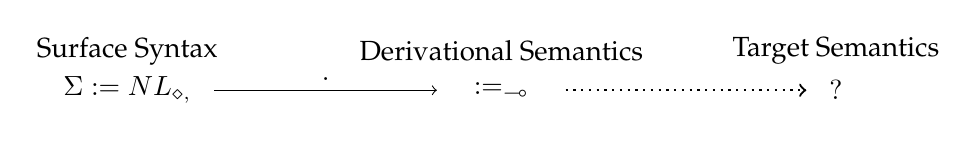
\begin{tikzpicture}
		\node	(ss)  at (0, 0.5) 	{Surface Syntax};
		\node[outer sep=5pt]	(nlp) at (0, 0) 	{$\Sigma := \logic{NL}_{\diamond,\bx}$};
		\node	(ds)  at (4.75, 0.5) 	{Derivational Semantics};
		\node[outer sep=10pt]  	(ill) at (4.75, 0) 	{$\Tau := \ILL_{\li}$};
		\draw[->] (nlp) -- node[above] {$\hm{.}$}  (ill) ;
		\node[outer sep=5pt] (target) at (9, 0)	{$?$};
		\node	(ts)  at (9, 0.5) 	{Target Semantics};
		\draw[->, dotted, thick] (ill) --  (target) ;
	\end{tikzpicture}
	\caption{The syntax-semantics interface in the type-logical setting.}
	\label{figure:synsemtlg}
\end{figure}

The homomorphism $\hm{.}$ operates on proofs, i.e. typed terms, and thus does double duty: it transforms both terms and types of $\Sigma$ to corresponding terms and types of $\Tau$.
It is handy, then, to define it on the basis of two components $\langle \eta, \theta \rangle$, where $\eta : \types^{\Sigma} \to \types^{\Tau}$ and $\theta: \terms^{\Sigma} \to \terms^{\Tau}$, such that $\hm{\smallterm{s}: \smallprop{A}} = \theta({\smallterm{s}}) : \eta({\smallprop{A}})$, where the typing relation at the right-hand side of the equation must hold (i.e. the two maps mutually respect derivability).
On the type level, $\eta$ must specify a pointwise mapping $\eta_0$ from the propositional constants $\propcon^{\Sigma}$ of the source logic to types $\types^{\Tau}$ of the intermediate logic.
In our case, we will consider this a bijection from $\propcon^{\Sigma}$ to $\propcon^{\Tau}$, such that $\eta_0(p) \mapsto p$ (i.e. instantiating $\propcon^{\Tau}$ as a literal copy of $\propcon^{\Sigma}$).
Then, to extend $\eta_0$ to $\eta$ we need to specify its action on complex types, where it essentially forgets the unary modalities and removes the directionality of the implications, as shown in Table~\ref{table:eta_nl}.
In the exact same vein, $\theta$ pointwise sends constants and variables to their copycat images, and is then inductively defined on complex terms, where it casts directional applications and abstractions to undirectional ones, drops modal decorations and performs the simplified substitution prescribed by the $\diamond E$ rule, as shown in Table~\ref{table:theta_nl}.
As an example, applying $\hm{.}$ to the proof of Figure~\ref{figure:lovecract_rel_clause} should yield the derivational term:
\begin{equation}\label{equation:litten_derterm}
\term{litten~(by~(that~(\lam \vari .(may~(never~(behold~\vari )))~(the~eye)))~(suns))}^{\prop{np}\li\prop{np}}
\end{equation}

\begin{table}[ht]
\begin{center}
	\begin{tabularx}{0.51\textwidth}{@{}c@{\quad$\mapsto$\quad}c@{}}
		\multicolumn{1}{@{}c}{$\types^{\Sigma}$} & \multicolumn{1}{c@{}}{$\types^{\Tau}$}\\
		\toprule
		$p \in \propcon^{\Sigma}$							& $\eta_0(p) := p \in \propcon^{\Tau}$\\
		$\smallprop{A}\divleft\smallprop{B}$,		
		$\smallprop{B}\divright\smallprop{A}$				& $\eta(\smallprop{A})\li\eta(\smallprop{B})$\\
		$\diamond\smallprop{A}$, 	$\bx\smallprop{A}$		& $\eta(\smallprop{A})$
	\end{tabularx}
	\caption{Translating $\NL_{\diamond,\bx}$ types to $\ILL_{\li}$.}
	\label{table:eta_nl}
\end{center}
\end{table}

\begin{table}[ht]
\begin{center}
	\begin{tabularx}{0.52\textwidth}{@{}c@{\quad$\mapsto$\quad}c@{}}
		\multicolumn{1}{@{}c}{$\terms^{\Sigma}$} & \multicolumn{1}{c@{}}{$\terms^{\Tau}$}\\
		\toprule
		$\w{c} \in \cons^{\Sigma}$							& $\theta_0(\w{c}) := \w{c} \in \cons^{\Tau}$\\
		$\smallterm{\vari } \in \vars^{\Sigma}$				& $\theta_0(\smallterm{\vari }) := \smallterm{\vari } \in\vars^{\Tau}$\\
		$\smallterm{s}\nappright\smallterm{t}$, 		
		$\smallterm{t}\nappleft\smallterm{s}$				& $\theta(\smallterm{s})~\theta(\smallterm{t})$\\
		$\lam\smallterm{\vari }.s$,
		$\adbmal\smallterm{\vari }.s$							& $\lam\theta(\smallterm{\vari }).\theta(\smallterm{s})$\\
		$\diaintro \smallterm{s}$, 
		$\boxintro \smallterm{s}$, 
		$\boxelim \smallterm{s}$							& $\theta(\smallterm{s})$\\
		$\caseof{\diaelim \smallterm{t}}{\smallterm{\vari }}{\smallterm{s}}$
															& $\theta(\smallterm{s})_{[\theta(\smallterm{\vari }) \mapsto \theta(\smallterm{t})]}$
	\end{tabularx}
	\caption{Translating $\NL_{\diamond,\bx}$ terms to $\ILL_{\li}$.}
	\label{table:theta_nl}
\end{center}
\end{table}

With the Curry-Howard isomorphism as our guiding star, there's no peril in navigating between syntactic and semantic theories.
Syntactic proofs are equated to syntactic terms, on which our homomorphism can be applied to yield derivational semantics terms, in turn equatable to derivational semantics proofs.
This might seem like a lot of work to simply ``forget'' syntax, but it showcases how one can step up the computational hierarchy of substructural logics in order to attain access to more expressive semantics.
Note also that such a path is merely a suggestion and not an imperative; a more ambitious line of though could maintain that word order variations (and the structural rules licensing them) can carry semantic cues which, albeit subtle, need to be upheld in the compositional meaning translation (see for instance  the contemporary work of \citet{duarte2022quantum} for some exotic interpretations of the control modalities).

\paragraph{The Role of the Lexicon}
The sentiments of the previous paragraph could be met with some skepticism.
A critical eye might argue that semantic interactions not already manifested in the syntax may never be born of this process, and thus wonder whether this added expressivity can serve any real purpose or offer any tangible benefits.
To dispel such doubts, we need to keep in mind that derivational terms refrain from specifying \textit{lexical meaning}, i.e. they treat lexical items as black boxes, from a semantic perspective.
Opening these black boxes would reveal flat entries (i.e. term constants) in the case of words providing meaning \textit{ingredients}, as opposed to structurally rich entries (i.e. complex terms with internal structure) in the case of words providing meaning \textit{recipes}.%
\footnote{This distinction is usually paralleled with the linguistic distinction between \textit{content} and \textit{function} words, but commiting to this being the case is an unecessary restriction. Depending on the end-target semantics logic and the granularity of the semantic lexicon, content words might still be assigned complex term structure -- a common trick, for instance, in delivering dependent type semantics; see the book of \citet{chatzikyriakidis2020formal} for an overview of recent developments.}
Structurally rich lexical entries can utilize \textit{any} term constructor made available by the semantic logic; crucially, this includes constructors that escape the narrow borders of the homomorphic codomain (i.e. do not have a syntactic origin).
Of course, such terms are still bound by the promise to obay the type dictated by the homomorphic translation of their original syntactic type, and must also be derivable theorems of the semantic logic they live in.
Increasing expressivity therefore may indeed not in itself add to the function/argument structures inherited by syntax, but provides the tools necessary for complex lexical semantic actions to take effect as needed.

A case in point is the coordinator \textex{and} conjoining the two modifiers of the previous section: \textex{litten by \dots \textbf{and} having in \dots}.
Each individual conjunct fulfills a descriptive filter that intersects the properties of its argument with the properties attributed by its internal meaning.
That is, of all objects of type $*$ (where $*$ an arbitrary type, denoting the interpretation target of $\smallprop{np}$), the first modifier withdraws all but those lit by unseeable suns, whereas the second one withdraws all but those with weird entities in their whirlpools.
For the full conjunction to have the intended meaning, i.e. evoke the image of exclusively this subset of oceans characterized by both the above properties, the coordinator would need to enact the role of a portable implementation of function composition%
	\footnote{Before anyone gets angry: I am neither pitching some provocative theory of conjunction semantics here,  nor secretly advocating for the dot-combinator -- just trying to make a point.} 
as in Figure~\ref{figure:funcomp}, so as to allow the iteration of the intersective modifiers:
\begin{equation}\label{equation:funcomp}
\lam \smallterm{\Var{0}\Var{1}\Var{2}.\Var{0}~(\Var{1}~\Var{2})} :: (*\li *)\li(*\li *)\li * \li *
\end{equation}
Even though no non-standard term constructors are to be found in this recipe, it is nontheless \textit{not} a theorem of the source logic, as function composition is not derivable in $\NL$.
In a set-theoretic semantics domain unbound by linearity constraints, another (perhaps more reasonable) translation might make use of an added operator $\wedge : * \to * \to *$ for set-theoretic intersection ($*$ now an arbitrary set), to deliver the recipe:
\begin{equation}
\lam \smallterm{\Var{0}\Var{1}\Var{2}.(\Var{0}~\Var{2})\wedge(\Var{1}~\Var{2})} :: (*\ii *)\ii(*\ii *)\ii * \ii *
\end{equation}

\subsection{Abstract Categorial Grammars}
\label{subsection:ACG}
So far, we have been predisposed to treating syntax as the hidden process that forms grammatically correct sentences.
It is insightful to contrast this treatment with the view of \citet{curry1961some}, who thought of syntax as a two-layered hierarchy of grammaticality criteria.
The deep layer, called \textit{tectogrammar}, would be concerned solely with the well-typedness of grammatical function domains and the validity of their interpretations.
The shallow layer, called \textit{phenogrammar}, would be where tectogrammatical proofs are transformed and cast to surface forms that abide by the linear order and constituency restrictions imposed by the language.
Type-logical grammars pose no challenge to the legitimacy of this distinction: it should be clear that phenogrammar, in Curry's terms, is our syntactic logic, and tectogrammar is what we earlier referred to as derivational semantics.
In being tectogrammar-first, however, they diverge in its operationalization.
The computational pipeline they propose is sequential in nature, and follows the Aristotelian path from observable evidence to latent variables: the surface string is perceived as the yield of a (shallow) syntactic proof, from which a deep semantic proof is extracted.
The operationalization closer to Curry would be inverted, placing phenogrammar at the top of the generative process, and following the Platonic information flow from deep and abstract to shallow and concrete.
This perspective is embodied by abstract categorial grammars~\cite{de2001towards} and their contemporary and closely related lambda grammars~\cite{muskens2001lambda}.
Both are tectogrammar-first formalisms that make use of $\ILL_{\li}$ and the Curry-Howard isomoprhism to obtain phenogrammatic realizations via homomorphic translations of the tectogrammatic parse.

\begin{figure}
	\centering
	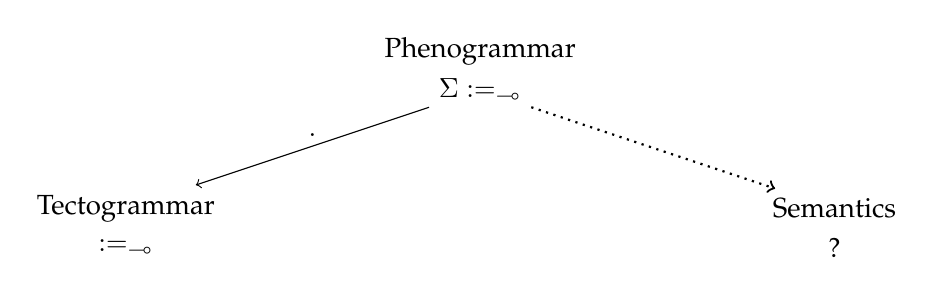
\begin{tikzpicture}
		\node (ds)		at (0, 2)		{Phenogrammar};
		\node (dsl)		at (0, 1.5)		{$\Sigma := \ILL_{\li}$};
		\node (ss)		at (-4.5, 0)		{Tectogrammar};
		\node (ssl)		at (-4.5, -0.5)	{$\Tau := \ILL_{\li}$};
		\node (ls)		at (4.5, 0)		{Semantics};
		\node (lsl)		at (4.5, -0.5)	{?};
		\draw[->] (dsl) -- node[above] {$\hm{.}$}  (ss) ;
		\draw[->,dotted,thick] (dsl) --	(ls) ;
	\end{tikzpicture}
	\caption{The syntax-semantics interface in the abstract categorial setting.}
	\label{figure:synsemacg}
\end{figure}

\subsubsection{Basic Definitions}
The focus of our presentation will be on abstract categorial grammars, as they are closer in spirit to what is to come later.
In its original definition, an abstract categoral grammar consists of two instantiations $\Sigma$, $\Tau$ of $\ILL_{\li}$, and a map between them.
The source instantiation $\Sigma$ provides a set of base types $\propcon^{\Sigma}$, and the so-called \textit{abstract vocabulary}: a set of \textit{abstract constants} $\cons^{\Sigma}$, each assigned a type from $\types^{\Sigma}$.
The target instantation $\Tau$ provides another set of base types $\propcon^{\Tau}$, and constants $\cons^{\Tau}$ with types from $\types^{\Tau}$, called the \textit{object vocabulary}.
The map between them is once again a homomomorphism $\hm{.}$, defined on the basis of $\langle \eta_0, \theta_0\rangle$.
Not unlike before, $\eta_0$ is seen as implementing a mapping $\propcon^{\Sigma} \to \types^{\Tau}$, and $\theta_0$ a mapping $\cons^{\Sigma}\to \terms^{\Tau}$, both pointwise defined.
Their homomorphic extension is trivially obtained by recursively defining their actions on implicational types, function terms and $\lam$ abstractions, where they simply mimic the source type- and term- structure.
This formulation lends itself nicely to the notion of \textit{grammar composition}, if one is to use the object logic of a grammar as the abstract logic of another.
Each grammar is accompanied by two \textit{languages}; the abstract language, i.e. the set of terms (of some \textit{distinguished} type $p_d\in \propcon^{\Sigma}$) derivable in the source logic, and the object language, i.e. the set of object terms the abstract language maps into.
For the phenogrammar to tectogrammar picture to be made evident, the distinguished type needs to be mapped to the functional string type $p_{d} \mapsto \mathtt{str}$, forcing terms of the object language to evaluate to strings.
Note that, despite appearances, $\mathtt{str}$ is a first-order type $*\li *$ (where $*$ some arbitrary primitive) so as to permit the view of string concatenation as function composition, identical to~(\ref{equation:funcomp}):
\begin{equation}
+ := \lam \term{\Var{0}^{\mathtt{str}}\Var{1}^{\mathtt{str}}\Var{2}^{*}.\Var{0}~(\Var{1}~\Var{2})}
\end{equation}


\subsubsection{Artificial Languages}
Abstract categorial grammars are characterized by two measures of complexity: the maximal order of source constants' types, and the maximal order of the codomain of $\eta_0$.
The two together constitute the grammar's \textit{class}, which concisely describes the sort of languages the grammar can model.
This can prove effective in revealing a more granular stratification underlying the Chomsky hierarchy of formal grammars, when the latter are embedded into abstract categorial equivalents; as such, the framework has found extensive use as a meta-language for the study and formalization of formal grammars (as done by \citet{de2004expressive}, \textit{inter alia}).
\footnote{There is a certain irony in formal grammars requiring or benefiting from formalization. If you're having trouble parsing this, consider that formal languages are essentially ad-hoc rules on strings; by formalization we mean giving these rules the type-theoretic treatment they deserve.}

To see this in practice, let's have some meta-fun pretty-printing the types of $\logic{(N)L}_{\diamond, \bx}$ by modeling their type formation rules (which constitute a context-free grammar) using an abstract categorial grammar.
First item on the agenda is the specification of our two logics $\Sigma$ and $\Tau$.
The source logic $\Sigma$ will provide the abstract backbone of the type grammar, containing a single base type, that of a well-formed ``type'' 
$\propcon^{\Sigma} := \{ \type[s] \}$.
The abstract vocabulary is then populated in Figure~\ref{figure:acg_nl_abstract_lex} by all abstract constants denoting base ``types''%
\footnote{In hindsight, that might have been an unfortunate choice of term\textsuperscript{\thefootnote} to overload.} and ``type'' constructors.
The target logic $\Tau$ will be our phenogrammatic printer tasked with translating abstract terms (``types'') to object terms (strings).
We will need a single object base type  $\propcon^{\Tau} := \{ * \}$, such that $\eta_0(\type[s]) = \mathtt{str}$, the type alias of $*\li *$.
Some auxiliary object constants are necessary before we proceed: opening and closing brackets, a diamond and a box the two implications, and a unique match for each unique \textit{constant} abstract constant (i.e. each abstract constant whose type is of order zero).
The above -- all of type $\mathtt{str}$, and underlined to distinguish from functional symbols -- are used by the abstract constant translation $\theta_0$ defined in Table~\ref{table:nl_tg_acg}: base constructors are mapped to their corresponding string representations, the two unary modalities simply concatenate their symbol to their single argument, whereas the two implications infix their arguments with the a slash or backslash, and wrap the result under brackets.

\begin{figure}
	\begin{align*}
	\cons^{\Sigma} := \{ 
		& 	\smallterm{n} :: \type[s],\ \smallterm{np} :: \type[s],\ \smallterm{pp} :: \type[s],\ \smallterm{np} :: \type[s],\\
		&	\smallterm{dia} :: \type[s]\li\type[s],\ \smallterm{box} :: \type[s]\li\type[s]\\
		&	\smallterm{ldiv} :: \type[s]\li\type[s]\li\type[s] \\
		&	\smallterm{rdiv} :: \type[s]\li\type[s]\li\type[s] \}
	\end{align*}
	\caption{Abstract lexicon for the language of $\logic{(N)L}_{\diamond, \bx}$ types.}
	\label{figure:acg_nl_abstract_lex}
\end{figure}

\begin{table}
	\centering
	\begin{tabularx}{0.75\textwidth}{@{}cc@{}}
		Abstract Constant							& Object Term\\
		\toprule
		$\smallterm{n}$								& $\underline{\smallprop{n}}$\\
		$\smallterm{np}$							& $\underline{\smallprop{np}}$\\
		$\smallterm{pp}$							& $\underline{\smallprop{pp}}$\\
		$\smallterm{s}$								& $\underline{\smallprop{s}}$\\
		$\smallterm{dia}$							& $\smallterm{\lam  \vari.\underline{\diamond} + \varj}$\\		
		$\smallterm{box}$							& $\smallterm{\lam  \vari.\underline{\bx} + \vark}$\\		
		$\smallterm{ldiv}$							& $\smallterm{\lam  \vari\varj.\underline{(} + \vari + \underline{\divleft} + \varj + \underline{)}}$\\
		$\smallterm{rdiv}$							& $\smallterm{\lam  \vari\varj.\underline{(} + \varj + \underline{\divright} + \vari + \underline{)}}$
	\end{tabularx}
	\caption{Object translation for the lexicon of Figure~\ref{figure:acg_nl_abstract_lex}.}
	\label{table:nl_tg_acg}
\end{table}

\begin{figure}
	{\smaller
	\[
		\infer[\li E]{\term{rdiv~(dia~(box~(ldiv~np~np)))~pp}:\type}{
			\infer{\type\li\type\li\type}{\term{rdiv}}
			&
			\infer[\li E]{\term{dia~(box~(ldiv~np~np))}: \type}{
				\infer{\type\li\type}{\term{dia}}
				&
				\infer[\li E]{\term{box~(ldiv~np~np)}: \type}{
					\infer{\type\li \type}{\term{box}}
					&
					\infer[\li E]{\term{ldiv~np~np}: \type}{
						\infer{\type \li \type \li \type}{\term{ldiv}}
						&
						\infer{\type}{\term{np}}
						&
						\infer{\type}{\term{np}}
					}					
				}
			}
			&
			\hspace{-45pt}
			\infer{\type}{\term{pp}}
		}
	\]
	}
	\caption{Constructing the type assignment of~(\ref{equation:litten}).}
	\label{figure:litten_acg_der}
\end{figure}

Figure~\ref{figure:litten_acg_der} presents the construction of the type previously assigned to \textex{litten}, $\diamond\bx (\np[s]\divleft\np[s])\divright\pp[s]$ (contexts are intentionally left empty and axioms replaced by abstract constants for brevity).
Applying the homomorphic translation to its abstract yields a printout in the form of the object term below (source function/argument brackets substituted with indendation levels for legibility):
\begin{equation}
	{
	\begin{aligned}
	& 			\hm{\term{rdiv~(dia~box~(ldiv~np~np)))~pp}}\\
	= \
	&				\smallterm{\lam  \vari\varj.\underline{(} + \varj + \underline{\divright} + \vari + \underline{)}}\\
	& \quad			\underline{\smallprop{pp}}\\
	& \quad 		\smallterm{\lam  \vark.\underline{\diamond} + \vark}\\
	& \qquad 		\smallterm{\lam  \varl.\underline{\bx} + \varl}\\
	& \qqquad		\smallterm{\lam  \Var{m}\Var{n}.\underline{(} + \Var{m} + \underline{\divleft} + \Var{n} + \underline{)}} \\
	& \qqqquad		\underline{\smallprop{np}}\\
	& \qqqquad		\underline{\smallprop{np}}\\
	\bredstar \
	&				\underline{(
						\diamond \bx ( \np \divleft \np )
						\divright \pp[s] 
						)}
	\end{aligned}
	}
\end{equation}
Six reduction steps later and... \textit{voil\`{a}} -- our pretty printer works!
The maximal order of the abstract constants is 1, and the maximal order of the translation is 2, making our grammar's complexity class (1, 2), a proper subset of the (2,2) that encapsulates context-free grammars.

\subsubsection{Human Languages}
Elegant and successful as they might be in their meta-theoretical enterprises, abstract categorial grammars have not fared as well with linguistic applications, in large part due to their computationally intractable nature.
On the one hand, they stand out from the rest of the categorial family in not being lexicalized by default.
The conceptual separation between lexicon and rules no longer holds: rules are fixed to the ones supplied by $\ILL_{\li}$, but inference is largely guided by the abstract constants.
Abstract constants may contain lexical items that make their way to the final (object) derivation, or simply compositional recipes that leave no imprint whatsoever.
At the same time, the framework is overly reliant on the constant map $\theta_0$ (defined on a per-item basis) for the translation into the object language to take effect.
Even in the lexicalized setup where the abstract lexicon is populated by words and words only, every abstract constant needs to be assigned both an abstract type and a unique object term for every phenogrammatic behavior it exhibits; two lexical dimensions, compared to the one of vanilla categorial grammars.
Enforcing grammaticality while blocking overgeneration of the object language similarly requires a careful, parallel finetuning of both the abstract language and the translation --  gone is the adage of words carrying their combinatorics on their sleeves. 
What's worse, words triggering higher-order tectogrammatic phenomena will then need object translations of an even higher order for their surface forms, making the design and population of a strict tectogrammatic translation $\hm{.}$ practically unfeasible.
This part could in principle be partially mitigated by flattening complex syntactic phenomena into lower-order (alias) types in the source domain, and outsourcing their expansion to a parallel grammar for concrete semantics -- this is less of a solution and more of a deferral, though.
Beyond issues of practicality, there are also foundational problems at stake, as resorting to a lexical enumeration of phenogrammatic forms evidences inability to perform linguistic generalization -- what \citet{moot2014hybrid} calls a problem of \textit{descriptive inadequacy} revolving around \textit{any} abstract replacement to a Lambek higher-order type.
Last but not least, it is hard to imagine an abstract categrial grammar in action: it is unclear how to procure an abstract proof object from the \textit{evaluated} yield of its object translation (i.e. the string form we are most likely encounter in the open) using traditional proof-theoretic disciplines -- the two layers of function/argument structures (abstract- and object- level) and their interacting reductions would unnerve even the sturdiest of parsers (or so it seems).

As an artificial yet illustrative and down-to-earth example, let's brave the design of an abstract categorial grammar tasked with the production of an end-to-end linguistic example.
Once more, we start with the specification of our two logics $\Sigma$ and $\Tau$.
For efficacy and simplicity, we can have $\Sigma$ coincide with the derivational semantics logic of Section~\ref{subsubsection:ssi_tlg}, inheriting its terms and types for free.
Doing so requires of course that we assume some high-level equivalence between the representations of what used to be abstract semantics before, and what now we call deep syntax -- let's naively take this for granted.
The object logic $\Tau$, being responsible for the surface materialization of our derivational proofs, will again need to be a logic of strings and is thus populated by a single atomic type $\propcon^{\Tau} = \{ *\}$; all abstract atoms atoms are then sent to $\mathtt{str}$.
For each word, we will need an abstract constant $\w{c} \in \cons^{\Sigma}$, and a corresponding object constant $\str{c} :: \mathtt{str} \in \cons^{\Tau}$, denoting the word's string form. 
Abstract constants will be sent to object terms via $\theta_0$, each of which must contain a single occurence of a term constant, in order to preserve lexicalism and respect lexical transparency.
Worth a special mention is the fact that the tectogrammatic image of words assigns them syntactic recipes, as they carry their own $\lam$ terms.
The story is summarized in Table~\ref{table:toy_acg_lexicon} (object types are ommitted for brevity -- simply substitute all atoms of the corresponding abstract types with $\mathtt{str}$ to obtain them).

\begin{table}[h]
	\centering
	\begin{tabularx}{0.85\textwidth}{@{}ccC@{}}
		Abstract Constant							& Abstract Type										& Object Term\\
		\toprule
		eye											& $\smalln$											& \str{eye}	\\
		suns										& $\smallnp$										& \str{suns} \\
		oceans										& $\smallnp$										& \str{ocreans} \\
		the											& $\smalln\li\smallnp$								& $\smallterm{\lam \vari.\str{the}+\vari}$\\
		opiate										& $\smallnp\li\smallnp$								& $\smallterm{\lam \vari.\str{opiate}+\vari}$\\
		poured										& $\smallnp\li\smalls$								& $\smallterm{\lam \vari.\vari + \str{poured}}$\\
		behold										& $\smallnp\li\smallnp\li\smalls$					& $\smallterm{\lam \vari\varj.\varj+\str{behold}+\vari }$\\
		there										& $(\smallnp\li\smalls)\li\smallnp\li\smalls$		& $\smallterm{\lam \vari \varj.(\vari~\varj) + \str{there}}$\\
		never										& $(\smallnp\li\smalls)\li\smallnp\li\smalls$		& $\smallterm{\lam \vari \varj.\str{never}+(\vari ~\varj)}$\\
		may											& $(\smallnp\li\smalls)\li\smallnp\li\smalls$		& $\smallterm{\lam \vari \varj.\str{may}+(\vari ~\varj)}$\\
		by											& $\np\li\pp$										& $\smallterm{\lam \vari.\str{by}+ \vari}$\\
		litten 										& $\smallpp\li\smallnp\li\smallnp$					& $\smallterm{\lam \vari\varj.\varj + \str{litten}+ \vari}$\\
		that										& $(\smallnp\li\smalls)\li\smallnp\li\smallnp$		& $\smallterm{\lam \vari\varj. \varj + \str{that} + \vari(\str{\gap})}$
	\end{tabularx}
	\caption{Abstract lovecraftian lexicon abiding to the types of Table~\ref{table:toy_lambek_lexicon}.}
	\label{table:toy_acg_lexicon}
\end{table}


The equation below shows the computation of the homomorphic translation to the derivational term (\ref{equation:litten_derterm}) inspected earlier.

{\smaller
\begin{equation}\label{equation:acg_pheno}
	\begin{aligned}
	& 			\hm{\term{litten~(by~(that~(\lam \vari .(may~(never~(behold~\vari )))~(the~eye)))~(suns))}} \\
	= \ 
	&							(\lam \vari\varj.\varj + \str{litten}+ \vari) \\
	&\quad								(\lam \vark.\str{by}+ \vark)\\
	&\qquad									(\lam \varl\varm. \varm + \str{that} + \varl(\str{\gap}))\\
	&\qqquad								(\lam x_n. \\
	&\qqquad\quad										(\lam x_o x_p.\str{may}+(x_o ~x_p))\\
	&\qqquad\qquad											(\lam x_q x_r.\str{never}+(x_q~x_r))\\
	&\qqquad\qqquad												(\lam x_sx_t.x_t+\str{behold}+x_s)\\
	&\qqquad\qqqquad												x_n \\
	&\qqquad												((\lam x_u.\str{the}+x_u)~\str{eye})\\
	&\quad									\str{suns}\\
	\bredstar \ & \term{\lam \vari.\vari + \str{litten}\str{by}\str{suns}\str{that}\str{the}\str{eye}\str{may}\str{never}\str{behold}}\str{\gap}
	\end{aligned}
\end{equation}
}%
This already proves quite an endeavour; twelve reduction steps later, we are presented with a seemingly reasonable output.
Upon closer inspection, though, an issue pops up: the end term is of type $\mathtt{str}\li\mathtt{str}$, making it an ill-fit for the discontinuous application to the \textit{substring} \str{opiate}\str{oceans}, which we expect to find nested within the main clause \str{opiate}\str{oceans}\str{poured}\str{there}.
For the tectogrammatical form to be able to surface correctly, some drastic adjustments are necessary.
We could alter the derivational proof by including non-lexical abstract constants, or refine the source types to impose (or enable) structural variation, but either option would be undermining the cohesion between deep syntax and semantics we started from.
The only alternative that does not resort to contaminating the original term -- abstract and pure -- with vulgar restrictions of form would be to lift the complexity of the interpretation and design it anew.

It seems therefore that the appealing simplicity and elegance of the tectogrammatic logic is counterbalanced by an increasingy bulky and cumbersome transition to the (equally simple, yet far less elegant) phenogrammatic logic.
The problem is of course more pronounced for natural languages, which overstep the strict confines of their formal counterparts~\cite{moot2014hybrid}.
If only we had a way to keep just the good part of a type-driven and semantically transparent deep syntax, without having to get involved with all the tedious labour of its surface materialization or the translation to it...
Spoiler alert: we will in a bit.

\subsection{Other Formalisms}
Type-logical and abstract categorial grammars have monopolized our interest, yet are not the only members of the categorial grammar family.
For the sake of completeness and impartiality, we will briefly discuss two other major flavours and contrast them to the ones so far presented.

\subsubsection{Combinatory Categorial Grammars}
A deviant from the categorial tradition are the broadly adopted combinatory categorial grammars~\cite{ades1982order,szabolcsi1989bound, steedman2022combinatory}.
These stray from the norm by rejecting the very idea of the syntactic variable (and with it, hypothetical reasoning), citing reasons of cognitive plausibility and parsing complexity.
Obviously, a categorial grammar stripped of hypothetical reasoning would not amount to much on its own: it would only be able to resolve syntactically flat sentences.
To regain some of the lost expressivity (ideally, exactly and only as much as needed), combinatory categorial grammars incorporate a collection of rules lent from the combinatory logic of~\citet{curry1958combinatory}, albeit in restricted form.
The first such rule is morpholexical in nature; it allows lexical items to raise their types once, before administering them to the syntactic derivation, forcing a flip in the local function/argument structure and allowing different semantic scopes to take effect as/when needed.
The remaining rules are essentially four instances of function composition -- one for each unique pair of directional implications considered.
The absence of hypothetical reasoning means that these are no longer derivable theorems of some underlying type theory, but ad-hoc schemata, fixed \textit{a priori} to fit their designated purpose.
To counteract overgeneration, these rules are made available only to a pre-defined subset of the sum of lexical types, empirically specified.
With respect to the interface, a combinatory derivaton can be cast into a semantic $\lam$ term the usual way; by assigning to each rule a corresponding term constructor.
Note, however, that this procedure is a non-invertible \textit{transformation} rather than an isomorphic correspondence; the purity of the Curry-Howard correspondence is lost, traded away for the aforementioned decrease in parsing complexity.

In spite of their (non-minor) differences, the agendas of multimodal type-logical grammars and combinatory categorial grammars are quite aligned, at least at a high level: they both stipulate the presence of syntactic universals that guide structure formation, utilize them as a pathway to semantics \textit{\`{a} la} Montague, and acknowledge the need for language-specific syntactic fine-tuning; one exercising proof-theoretic control via unary type operators and structural rules, the other controlling the applicability of the so-called combinatory rules via lexical adjustment.
For better or worse, combinatory categorial grammars have taken the lion's share of the practitioners' focus: they boast an assortment of tools and annotated corpora across languages, the size of which far exceeds that of their less popular siblings -- to the point where the term categorial grammars has become an almost synonym of combinatory categorial grammars.%
\footnote{At least if one is to consider the reviewers I get assigned a reliable statistical sample of the NLP population.}
I hope that, by its end, this thesis will have slightly adjusted the scales towards a healthier epistemological pluralism.

\subsubsection{Hybrid Type-Logical Grammars}
In the lands between type-logical grammars and their abstract siblings, there lives the strangeness of hybrid type-logical grammars.
Originally proposed by~\citet{kubota2012gapping}, hybrid type-logical grammars utilize a combination of the two slashes of traditional Lambek calculi with the non-directional linear implication, to give birth to a type grammar that combines the good aspects of both approaches while purportedly suffering the restrictions of neither.
The types of a hybrid type-logical grammar are the result of two stages of induction.
The first stage creates standard Lambek types, as in~(\ref{equation:LC}).
The second stage is of the form 
\begin{equation}
	\prop{a}, \prop{b}, \prop{c} := \prop{l} \ | \ \prop{a} \li \prop{b}
\end{equation}
where $\smallprop{l}$ a valid Lambek type.
The term calculus of hybrid type-logical grammars requires a translation of logical types into so-called \textit{prosodic} types $\smallprop{st}$ (for structure or string), such that all stage 1 (Lambek) types are sent to $\smallprop{st}$, and stage 2 types are inductively translated as (higher-order) functions over $\smallprop{st}$. 
The term constructors assigned to the elimination (resp. introduction) of the Lambek connectives is that of structure concatenation (resp. separation), whereas the term constructors assigned to the linear connective are standard function application and variable abstraction.
The marriage of these two layers of abstraction in the same term calculus might seem unorthodox or at least aesthetically displeasing, but is not without merit.
Concetenative terms allow the framework to relax the lexical pressure of an abstract categorial grammar by preserving the canonical categorial grammar treatment of local syntactic phenomena.
Applicative terms constitute localized and controlled bursts of ad-hoc expressivity that can exceptionally allow the derivation of higher-order and non-local phenomena normally inacessible to the OG Lambek calculi.
Hybrid type-logical grammars are a relatively new addition to the family, and are subject to ongoing research, both from the linguistic and the proof-theoretic perspective~\cite{kubota2020type,moot2022logical}.
As to why one would choose this setup over alternatives, your guess is as good as mine; hybrid proponents proclaim the system less obscure and more fit for linguistic applications~\cite{kubota2020type} -- external validation is still pending.


\section{Key References \& Further Reading}
Key references for this chapter were the Stanford Encyclopedia of Phisolophy entry on type-logical grammars~\cite{sep-typelogical-grammar} and the tried-and-true extended introduction books on $\lambda$-calculi and type theories of \citet{sorensen2006lectures} and \citet{pierce2004advanced}.
Moral credit is owed to my once faithful travel companion, the categorial grammar bible of \citet{moot2012logic}; it provides an accessible yet detailed documentation of most of the concepts hinted at in this chapter.
Sections~\ref{section:simple_type_theory} and~\ref{section:linear_type_theory} draw heavily, both in content and in style, from the excellent tutorial paper of \citet{wadler1993taste} on linear type theory -- waning presentational influences might be discernible up to Section~\ref{section:modalities}.

If unhappy about this chapter ending, or unsatisfied with the exposition provided, here's some extra reading material to keep you company.
For a detailed inquiry on proof nets and their linguistic applications, or an exemplar of what an actual great dissertation looks like, take a look at my co-supervisor's one~\cite{moot2002proof}.
For a more mathematically eloquent presentation of modalities and their potential as tools of inferential and structural reasoning, refer to the (also superb) dissertation of~\citet{bernardi2002reasoning}.
For a slightly outdated but still very educative overview of abstract categorial grammars, the lecture notes of~\citet{kanazawa2009advances} should prove handy.
If your eco-conscious side was moved by linear logic, but you find yourself lacking the bravery of facing the original manuscript of \citet{girard1987linear}, the lecture notes of \citet{troelstra1991lectures} would make for a good alternative.
If on the other hand you were intrigued about the vast expanse of type theories beyond the tiny scope of this thesis, the entry point to the downwards descent into the rabbit hole should be the seminal work of~\citet{martin1982constructive}.
A convincingly easy-to-swallow application of such type theories in the formal semantics world is extensively summarized by \citet{chatzikyriakidis2020formal}.
If you do like formal semantics but big lambdas give you nausea, there's a broad selection of books to go for; I still find myself guiltily cross-checking definitions and examples with that of \citet{winter2016elements} at times.
Finally, if what caught your attention was the historical drama at the beginning of the chapter, you will enjoy reading about the history of constructivism by \citet{troelstra2011history}.


\bibliographystyle{abbrvnat}
\bibliography{bibliography}

\chapter{Typing Dependency Structure}
\label{chapter:chapter_2}

\chapabstract{
	Predicates are functors,\\
	complements -- diamonds,\\
	adjuncts -- boxes;\\
	Everything a type.
}

The previous chapter initiated us into the history-rich world of substructural logics in the intuitionistic tradition.
Along the (artificially homogenized) story, we got to dip our toes into linguistic waters, where we saw these logics thrive and prosper, finding their place as the foundation for categorial grammars.
The many flavours of categorial grammars all have a single common denominator: they treat syntax as a hierarchical structure that puts phrases together from small to big, starting from words and reaching up to the sentence, the imprint being a natural deduction tree (and perhaps a phrasal bracketing structure).
This emphasis on the phrase, combined with the distinctive shape of the categorial parse, allows for a partial parallel to be drawn between categorial grammars and phrase structure grammars, despite their stark methodological and theoretical contrasts.
Phrase structure grammars are rule-based systems that assign categories to phrases according to their syntactic function, and manipulate phrasal formation by specifying how their constituent parts combine -- the produce being a bracketing structure, commonly visualized in tree format.
A different approach to grammatical theory abandons the constituency relation, adopting the dependency relation in its stead.
Dependency relations do not seem compatible with the categorial setup at a first glance: they are flat, and lack the notion of finite phrasal parts -- in showing no attachment to iterative phrasal division, they are also not obviously compositional.

In this, chapter we will focus our efforts into bridging this gap between these two perspectives under a unified categorial grammar setup.
We will motivate the incorporation of dependency relations into the categorial vocabulary by repurposing existing and well-studied tools that remain faithful to the type theory roots the previous chapter has established (spoiler: it's the modalities).
We will finally discuss how their inclusion alters the structural paradigms of the previous chapter, and the opportunities and problems this change comes with.

\section{Phrase vs. Dependency Structure}
\label{section:phrase_vs_dependecy}
Before we get to theorycrafting, it would be useful to try and clarify what exactly is meant by constituency- and dependency- structure, and how the two differ.

\subsection{Phrase Structure Grammars}
Phrase structure grammars build on the observation that certain phrases seem to act as rigid and independent chunks, sometimes referred to as \textit{constituents}. 
Viewed from within, these phrases may be rich in internal structure, but keep it sealed off to the outside.
Viewed externally (i.e. in the context of a wider phrase that contains them), they are indivisible units, at least for the purposes of phrasal composition.
Phrases are inventorized according to their syntactic \textit{categories}.
If one so wishes, one can for the most part replace a phrase for another of the same category, with no effect to grammaticality or local structure, which suggests they are functionally indiscernible.
The examples below testify to this%
\footnote{Sourced from H.P. Lovecraft, \textit{Celepha\"{i}s}  (1922). In \textit{The Rainbow, vol. 2.}}; the underlined phrases can be freely interchanged -- despite their wildly different internal structures, substituting one for another has no effect on the outer sentential structure:

{\smaller%
\begin{enumerate}
\item $\w{he}\sbind(\w{beheld}\sbind\underline{(\w{the}\sbind\w{city})})$
\item $\w{he}\sbind(\w{beheld}\sbind\underline{(\w{the}\sbind((\w{glittering}\sbind{\w{minarets}})\sbind(\w{of}\sbind(\w{the}\sbind\w{city}))))})$
\item $\w{he}\sbind(\w{beheld}\sbind(\underline{(\w{such}\sbind\w{beauty})\sbind(\w{of}\sbind((\w{red}\sbind(\w{and}\sbind\w{white}))\sbind\w{flowers})))})$
\item $\w{he}\sbind(\w{beheld}\sbind(\underline{
	(
		\w{some}\sbind
			(\w{feature}\sbind
				(\w{or}\sbind\w{arrangement})
			)\!\sbind\!
			(\w{which}\sbind
				(\w{he}\sbind
					(
						(\w{had}\sbind\w{known})\sbind
						\w{before}
					)					
				)
			)})$
\end{enumerate}}%

\noindent These so-called constituents interact, then, with one another depending not on their contents, but rather their categories.
This perspective promotes a disciplined approach to grammar modeling, dating back to the formal grammars of \citet{chomsky1956three}, the archetypical example being context-free grammars~\cite{chomsky1956three,jw1959c}.
There, the construction of complex expressions is guided by \textit{production rules}, grammatical recipes that dictate what categories can sequentially combine, in what order, and what the category of their combination is.
The above example would correspond, for instance, to production rules of the form:
\begin{align}
	S 	& 	\to NP \ VP \label{equation:sfromnpvp}\\
	VP 	&	\to TV \ NP \label{equation:vpfromtvnvp}
\end{align}
claiming that one of the ways to make a verb phrase $VP$ involves concatenating a transitive verb $TV$ with a noun phrase $NP$, which in turn can be plugged to the right of another $NP$ to produce a declarative sentence $S$ -- each rule leaving a bracketing structure (or binary tree) in its wake (see Figure~\ref{subfigure:cfgtree}).


\begin{figure}
	\centering
	\hfill%
	\begin{subfigure}[b]{0.35\textwidth}
		\begin{tikzpicture}
			\Tree 
				[ .{$S$} 
					[.{(\ref{equation:sfromnpvp})}
						[.{$NP$} 
							\w{he} 
						] 
						[.{$VP$}
							[.{(\ref{equation:vpfromtvnvp})} 
								[.{$TV$} \w{beheld} ] 
								[.{$NP$} 
									\edge[roof]; {\dots} 
								] 
							]
						] 
					]
				] 
		\end{tikzpicture}
		\caption{Context-free parse tree.}
		\label{subfigure:cfgtree}
	\end{subfigure}\hfill%
	\begin{subfigure}[b]{0.45\textwidth}
		\begin{tikzpicture}
			\Tree 
				[ .\s[s]
					[.{$\appleft$}
						[.{\np[s]}
							\w{he}
						]
						[.{$\np[s]\divleft\s[s]$}
							[.{$\appright$}
								[.{$(\np[s]\divleft\s[s])\divright\np[s]$} \w{beheld} ]
								[.{\np[s]}
									\edge[roof]; {\dots}
								]
							]
						]
					]
				]
		\end{tikzpicture}
		\caption{Tree-formatted Lambek derivation.}
		\label{subfigure:lambektree}
	\end{subfigure}\hfill
	\caption{A phrase-structure grammar parse tree (\subref{subfigure:cfgtree}) contrasted with a Lambek abstract syntax tree (\subref{subfigure:lambektree}).}
	\label{figure:cfgvslambek}
\end{figure}

Even though context-free grammars are no longer seriously considered in the linguistic world, they have directly influenced most early attempts at grammar design -- and, by extension, their later successors and refinements.
Notational evidence of this past are more than noticeable today, ranging from the wide adoption of tree-style notation for syntactic analyses to the conceptual syncretism of constituency grammars and phrase structure ones.
More up-to-date frameworks expand upon the barebones context-free backend with niceties like a separation of functional dominance and linear precedence, added rules that manipulate movement and discontinuity, the proclamation of a single category as the \textit{head} of a production rule (or subtree), feature markings that carry semantic, morphological or phonological information, incorporation of dependency information, etc.~\cite[inter alia]{gazdar1985generalized,jacobson1987phrase,pollard1994head,dalrymple2001lexical}.

\hide{To our ill fortune, the field of formal syntax is actually an informal mess, more akin to a mine field rather than an academic one; it's best if I tread carefully and refrain from overextending myself here, in order to avoid setting off unseen traps or causing easily avoidable confusion.}
The point I want to make is that the focal center of the above formalisms is the \textit{phrase} and its structure -- as such, they are all referred to as phrase structure grammars, regardless of whatever extra fluff they carry or what their expressive capacity is.
In that broader sense of the term, and removing any implicit connotations of intellectual lineage, categorial grammars can also be conceived as phrase-centric.
Pure Lambek systems, for one, also explicate how phrases are combined, adhere to hierarchical forms similar to those of context-free grammars (except beautifully, see Figure~\ref{subfigure:lambektree}) and in fact have the same expressive capacity with respect to string formation (i.e. the two are \textit{weakly} equivalent)~\cite{pentus1993lambek}.
Categorial grammars abstract away from the rule inventory by utilizing the smallest and purest set of rules possible -- those of function application and variable abstraction -- and internalize what used to be rule-imposed structure within the lexical categories themselves.
Bracketing structure is now the footprint of function application, and the interface with semantics is naturalized by virtue of the Curry-Howard correspondence, as we saw earlier.
Rather than a $VP$ category and rule~(\ref{equation:sfromnpvp}), we have the \textit{type} $\np[s]\divleft\s[s]$ -- transparent with respect to both its syntactic combinatorics and semantic function.
Performing the function application on a left-adjacent \np[s] will then result to a local tree structure, not unlike the corresponding production rule -- see Figure~\ref{figure:cfgvslambek} for a comparison.
Note that in reality, categorial derivations in the type-theoretic tradition resemble trees only locally, since in high-order phenomena involving abstractions the unary, non-terminal $\lambda$ nodes will either need to be uniquely named with the variable they are binding, or otherwise point to it  with an additional edge -- hence a directed acyclic graph could make for a more accurate representation format.
Long story short, even without extensions to the logical core for managing discontinuity, calling deductive parsing constituency parsing would obviously not be doing the former justice; yet despite their methodological and theoretical divergences, their end yield is comparable -- the antecedent structures of Figures~\ref{figure:nl_applicative_examples} to~\ref{figure:lovecraft_coord} testify that the former may in fact be seen as subsuming the latter.

\subsection{Dependency Grammars}
\label{subsection:dep_grammars}
The constituency tradition has co-evolved along the opposing view of dependency grammars~\cite[inter alia]{tesniere2015elements,gaifman1965dependency,sgall1986meaning,mel1988dependency,sleator1995parsing}.
Dependency grammars reject the binary phrasal division that constituency grammars abide by, and instead adopt a flatter structural form, the only unit of which is the word.
Words are connected with one another by dependency arcs, i.e. directed edges between word pairs.
Each word can have arbitrarily many outgoing edges (dependents), but only a single incoming edge (head) -- the exception is the root word which has no head of its own (i.e. the head of the matrix clause).
A word is said to directy dominate its dependents, and indirectly dominate all words its dependents dominate (directly or otherwise) -- e.g. the root indirectly dominates every other word in the sentence.
This distinction between head and dependent is central to dependency grammars; broadly speaking, heads can be thought of as the words that decide the syntactic functionality of the collection of words (for fear of calling it a phrase) they indirectly dominate.
The dependency structure of a sentence is once more a tree, with words now as both terminal and non-terminal nodes, glued together with dependency relations.
A dependency tree is unconstrained by adjacency and word order: edges can fly over other edges; planarity is optionaly respected: an edge penetrating another edge to enter a nested domain is called \textit{non projective}.
This perspective is computationally appealing due to its simplicity and uniformity, as it allows a dependency grammar to argue about languages with wildly diverging syntactic and typological properties while remaining virtually unchanged.
For the exact same reasons, it can also be seen as concealing -- it sacrifices any potential of targeted analysis in the pedestal of universality.
Finally, the semantically inclined might find a two-directional extension of dependency arcs enticing.
In that setup, the added direction (which needs not agree with that of syntactic dominance) is devoted to semantic information flow, pointing from semantic predicates%
	\footnote{Apparently also an overloaded term. I will only ever use this in the strictly logical sense.},
to semantic arguments~\cite{mel2003levels}.

A dependency grammar that has gained significant traction over the last decade is the framework of universal dependencies (UD)~\cite{10.1162/coli_a_00402}, claiming a broad collection of multi-lingual treebanks~\cite{nivre2020universal} and tools.
In UD, words are usually assigned a label pulled from a rudimentary set of part of speech tags and lexical identifiers; more importantly, dependency relations are also labeled according to their grammatical function, allowing the distinction of a words' dependents according to the grammatical role they fulfill.
Grammatical roles are typologically and thematically informed, and are inventorized with language universality as the prime goal.
This inventorization upholds no semantic promises, but is not inconsistent with the aforementioned semantic view either.
To obtain a semantic transcription of the dependency tree, one needs only specify whether the semantic flow of each grammatical role is co- or contra- directional to the edge's syntactic flow, i.e. whether the arc marks its dependent as a \textit{complement} (where syntactic head and semantic predicate coincide) or an \textit{adjunct} (where the syntactic head is the semantic argument to its syntactic dependent).%
	\footnote{UD explicitly refuses to make this claim, as complements and adjuncts are largely language-particular syntactic constructs and a notorious point of debate~\cite{haspelmath2014arguments}.
	I would like to believe I am not trespassing here, either -- as will be made clearer in a bit, I employ the two terms in a purely semantic fashion.}

\begin{figure}
	\centering
	\begin{tikzpicture}[t/.style={text height=1.5ex, text depth=.25ex, rectangle, outer sep=0pt}, node distance=10pt]
	\smaller
	\node[t] (he) 			at (0, 0) {\w{he}};
	\node[t] (he_)			[below=4pt of he] {\w{PRON}};
	\node[t] (beheld)		[right=10pt of he] {\w{beheld}};
	\node[t] (beheld_)		[below=4pt of beheld] {\w{VERB}};
	\node[t] (the) 			[right=10pt of beheld] {\w{the}};
	\node[t] (the_)			[below=4pt of the] {\w{DET}};
	\node[t] (glittering) 	[right=10pt of the] {\w{glittering}};
	\node[t] (glittering_)	[below=4pt of glittering] {\w{VERB}};
	\node[t] (minarets)		[right=10pt of glittering] {\w{minarets}};
	\node[t] (minarets_)	[below=4pt of minarets] {\w{NOUN}};
	\node[t] (of)			[right=10pt of minarets] {\w{of}};
	\node[t] (of_)			[below=4pt of of] {\w{ADP}};
	\node[t] (the2)			[right=10pt of of] {\w{the}};
	\node[t] (the2_)		[below=4pt of the2] {\w{DET}};
	\node[t] (city)			[right=10pt of the2] {\w{city}};
	\node[t] (city_)		[below=4pt of city] {\w{NOUN}};
	\draw[->] (beheld) [bend right=80] edge node [above] {\smaller[2]{nsubj}} (he);
	\draw[->] (beheld) [bend left=90] edge node [above] {\smaller[2]{dobj}} (minarets);
	\draw[->] (minarets) [bend right=40] edge node [above] {\smaller[2]{amod}} (glittering);
	\draw[->] (minarets) [bend right=70] edge node [above] {\smaller[2]{det}} (the);
	\draw[->] (minarets) [bend left=60] edge node [above] {\smaller[2]{prep}} (of);	
	\draw[->] (of) [bend left=90] edge node [above] {\smaller[2]{pobj}} (city);	
	\draw[->] (city) [bend right=60] edge node [above] {\smaller[2]{det}} (the2);
	\end{tikzpicture}
	\caption{A sample dependency parse in the universal dependencies format.}
	\label{figure:udparse}
\end{figure}

Figure~\ref{figure:udparse} shows an example dependency parse.
Unlike before, we can not claim any semblance to the proofs that have occupied us thus far.
At a first glance, dependency grammars have little in common with categorial grammars -- structures are no longer binary nor made out of phrases, the axis of grammatical functions is competely new, and there seems to be little there reminiscent of the notions of induction and composition.
Though on closer inspection and armed with some goodwill, we can recover from some of these divergences if we make a few concessions from both sides.
We can start by treating any collection of words rooted in the same ancestor in the dependency tree as a constituent phrase, albeit possibly discontinuous -- the result will give us at least some partial overlap with the categorial directive.
Grammatical functions can then be thought of as being implicit, having been internalized in their positioning within a functor.
For instance we do intuitively know that the Lambek transitive verb $(\np[s]\divleft\s[s])\divright\np[s]$ requires an \textit{object} $\np[s]$ to the right and a \textit{subject} $\np[s]$ to the left -- marking them as such is perhaps redundant, since the verbal meaning recipe places each syntactic argument into a distinct semantic slot.
The binary bracketing structure is irrevocably lost, but this loss can be deemed as inconsequential if we ``flatten'' functor-induced phrasal boundaries by considering them only at these intermediary points where all of their arguments (however many) have been applied.
It is not much further we can get with this mediatory role, though.
No concession from the categorial side would be able to justify the underspecification of higher-order phenomena in a dependency tree,
and no concession from the dependency side could make peace with the omission of the concept of headedness in an applicative natural deduction proof.

\section{Modalities for Dependency Demarcation}
\label{section:modalities_for_dependency}
In our new quest, we will seek to design a type logic that subsumes and rises above both phrase structure grammars and dependency grammars.
As we saw in the previous section, the bar is not set particularly high for the first kind; the Lambek calculus can already do more than well enough.
The challenge then is to integrate the added values of a dependency grammar in a type-theoretic framework.
There's two elements we are missing; distinguishing between syntactic heads and syntactic/semantic predicates, and marking words and phrases according to their grammatical roles within some wider context.

\subsection{Two Dimensional Predicates}
Categorial grammars are inherently and by design biased towards predicate structures, primarily syntactic, but simultaneously also semantic (if one is to believe the story of Section~\ref{subsubsection:ssi_tlg}, no distinction can be made between the two).
Each phrase can be iteratively split apart into two subphrases (not necessarily contiguous), where one provides a functor, and the other the argument thereof.
Note that this distinction does not preclude the possibility that the argument itself has a functional type -- no assumption is made on the form of either subphrase's type, other than the two being compatible.
But what assumes the role of the functor in a local domain needs not always be the syntactic head of that domain.
There's a plethora of example cases.
Quantifiers, for one, are inarguably predicates over the objects they quantify, yet they exactly obey the morphosyntactic characteristics prescribed by these objects (i.e. grammatical gender, case, number, etc.), evidencing that the latter are in fact the heads -- a clear violation of any alignment we could ever hypothesize between functional predicateness and syntactic headedness.
A similar argument can be made for determiners and, more broadly speaking, any phrasal element that takes functional precedence without being the syntactically prominent part of its phrase, e.g. adjectival and adverbial modifiers.

This observation gives rise to a binary subcategorization of a binary predicate structure; to establish some risky terminology, it is either:
\begin{enumerate}
	\item an application of a head to its \textit{complement}, or
	\item an application of an \textit{adjunct} to its head
\end{enumerate}
where the distinction between complement and adjunct is made solely on the basis of their functional relation to the head.

The vanilla categorial vocabulary does not suffice to capture this extra dimension of function application\hide{ -- a problem also noticed by the intellectuals of proto-categorial civilizations, as archeological excavations reveal}.
In an unpublished manuscript, \citet{moortgat1991heads} propose a bidimensional implicational type operator and corresponding residuation laws: the first binary dimension is reserved for the usual left- vs. right- application distinction, whereas the second binary dimension specifies whether the head occurs to the left or to the right; the result is four unique ways of building up an implication.
Congruent with the substructural trend of revealing structure that was once hidden, this division brings forth a two-valued structural binder, allowing the corresponding logic $\logic{DNL}$ to reason about \textit{headed} binary trees.
The authors refrain from commiting to a specific linguistic application, but, translated into our terminology, their proposal can be schematically summarized by Figure~\ref{figure:heads_and_phrases}.
Further away from syntax, \citet{hendriks1997logic} employs \logic{DNL} to account for prosodic structures, where the head is assigned to intonationally prominent elements.

\begin{figure}
	\centering
	\begin{tabularx}{0.7\textwidth}{@{}lXr@{}}
	\begin{tikzpicture}[level distance=60pt, sibling distance=30pt,
						t/.style={text height=1.5ex, text depth=.25ex, rectangle, outer sep=0pt}, node distance=10pt]
	\Tree [.{$\prop{b}$} \edge[head] node[midway,left,t]{$\textit{head}$}; {$\prop{b}\divright_l\prop{a}$} \edge node[midway,right,t]{$\textit{complement}$}; {$\prop{a}$} ]
	\end{tikzpicture}
	&
	&
	\begin{tikzpicture}[level distance=60pt, sibling distance=30pt,
						t/.style={text height=1.5ex, text depth=.25ex, rectangle, outer sep=0pt}, node distance=10pt]
	\Tree [.{$\prop{b}$} \edge node[midway,left,t]{$\textit{complement}$}; {$\prop{a}$} \edge[head] node[midway,right,t]{$\textit{head}$}; {$\prop{a}\divleft_r\prop{b}$} ]
	\end{tikzpicture}\\[\smallsep]
	\begin{tikzpicture}[level distance=60pt, sibling distance=30pt,
						t/.style={text height=1.5ex, text depth=.25ex, rectangle, outer sep=0pt}, node distance=10pt]
	\Tree [.{$\prop{b}$} \edge[head] node[midway,left,t]{$\textit{head}$}; {$\prop{a}$} \edge node[midway,right,t]{$\textit{adjunct}$}; {$\prop{a}\divleft_l\prop{b}$} ]
	\end{tikzpicture}
	&
	&
	\begin{tikzpicture}[level distance=60pt, sibling distance=30pt,
						t/.style={text height=1.5ex, text depth=.25ex, rectangle, outer sep=0pt}, node distance=10pt]
	\Tree [.{$\prop{b}$} \edge node[midway,left,t]{$\textit{adjunct}$}; {$\prop{b}\divright_r\prop{a}$} \edge[head] node[midway,right,t]{$\textit{head}$}; {$\prop{a}$} ]
	\end{tikzpicture}\\
	\end{tabularx}
	\caption{The four implications of \logic{DNL}.}
	\label{figure:heads_and_phrases}
\end{figure}

\subsection{Modal Dependents}
As an alternative to introducing implicational (and by residuation, product) variants, we can instead opt for the more fashionable modal decomposition approach~\cite{kurtonina1997structural}.
The allows us to view a specialized (here: head-aware) implicational variant as a composition of its uniform base with a unary modality.
The standard route would have use the modality to mark the head -- we will instead mark the dependent.
\hide[T]{More than a petty act of rejection to establishment, t}his shall provide us with the means to further differentiate dependents according to the exact grammatical slots they occupy -- after all, there's quite a few different dependency labels, but only the one head.

\subsubsection{Complements vs. Adjuncts}
Sticking to our risky agenda, the first distinction we need to make is that of complements versus adjuncts.
In the complement case, such a decomposition would look as follows:
\begin{align}
	\prop{b} \divright_l \prop{a} \ \equiv \ \prop{b} \divright \diamond \prop{a} \\
	\prop{a} \divleft_r \prop{b} \ \equiv \ \diamond  \prop{a} \divleft \prop{b}
\end{align}
The translation is straightforward: predicates in head position are functors requiring the same arguments as they would before, except now under a diamond.
In that sense, they \textit{assign} diamonds to their complements by necessitating an application of the $\diamond I$ rule of Figure~\ref{figure:modal_logical} prior to the function application.
Recalling the structural imprint of the rule, this results in an extra layer of bracketing structure the delimits complement phrases and isolates them from their surroundings.

The adjunct case may at first glance seem slightly more obscure.
Following the directives of the previous paragraph, we need to mark the dependent -- this time a predicate in non head position -- in a way such that its application on its argument leaves a bracketing imprint on the structure of the former instead of the latter.
The solution manifests itself in the form of a box:
\begin{align}
	\prop{b} \divright_r \prop{a} \ \equiv \ \bx (\prop{b} \divright \prop{a}) \\
	\prop{a} \divleft_l \prop{b} \ \equiv \ \bx (\prop{a} \divleft \prop{b})
\end{align}
The translation is not much different: adjuncts are predicates wrapped by a box.
To reveal the pure function contained therein and allow a proof to progress, we need to invoke the $\bx E$ rule of Figure~\ref{figure:modal_logical}, the effect being a bracketing structure that now delimits adjunct phrases.

There is symmetry between the above two cases.
The task of imposing dependency structure is always upon the functional predicate and its type.
Head predicates mark their complements, whereas adjunct predicates mark themselves; in either case, it is the dependent structure that gets the brackets.
The duality of predicate structure is thus mirrored in the innate distinction between function and argument of the applicative categorial backend, whereas the duality of syntactic headedness is captured by the unary modalities; type-checking in both dimensions.

\subsubsection{Grammatical Functions}
Let's take this a bit further.
Universal dependencies may make no adjunct vs. complement distinction, but they go the extra mile of subspecifying dependents according to the exact grammatical roles they play.
Extending our grammar logic accordingly is straightforward.
Rather than have a single diamond and box, we can consider a usecase where modalities are a \textit{family} of unary residuals, i.e. a set of pairs, each labeled according to a single, unique dependency label.
The generalization is a multimodal type system consisting of modal pairs:
\begin{equation}
\{(\ddia{d}, \dbox{d}) \ | \ {\dep{d} \in \deps} \} 
\end{equation}
where \deps{} the full set of dependency labels made available to each specific instantiation of the theory.%
\footnote{Note that the label set can vary depending on the designer's end goal; grammatical functions is just one of the possibilities.
	The setup is also more than compatible with frame semantics, where event-specific semantic structures (\textit{frames}) are evoked by lexicalized syntactic heads to assign semantic/thematic roles to their dependents (\textit{frame elements})~\cite{fillmore1976frame}.}%
The edge case of \deps{} being a singleton set collapses to the previous exposition (whereby explicit labeling is redundant).

Each instance of a labeled modality will now come with its own introduction and elimination rules.
Concomitantly, both the term calculus and the bracketing structures are extended with multiple labels; the modal rewrites and unary brackets of Section~\ref{subsec:modal_logic} are now differentiated on the basis of the dependency label that induced them.
Unlike before, the structural effect is not a means to the end of structural reasoning, but the very purpose of the dependency modalities -- as such, they are not necessarily associated with any structural rules (even though nothing precludes the possibility -- it might even be reasonable to condition each dependency or combinations thereof to a unique set of structural transformations, as we will see in a bit).
Note, also, that the residuation properties and normalization routines apply only between diamonds and boxes of the \textit{same label} -- no interaction between mismatched types and terms is stipulated.


\subsection{Inference with Dependency-Enhanced Types}
Logical inference in the setup envisaged here is not dissimilar conceptually to the standard type-logical pipeline of Section~\ref{subsection:typelogical}, but there's some crucial differences that require explication, plus a few critical gotchas to beware of.

\subsubsection{Initial Lexical Adjustments}
For starters, functors previously involved with simple applicative phenomena will now need to abide to either of the type patterns below:
\begin{equation}\label{equation:dependency_functors}
	\prop{a}, \prop{b} := \ddia{d}\prop{a} \divleft \prop{b} \ | \ \prop{b}\divright \ddia{d}\prop{a} \ | \  \dbox{d}(\prop{a}\divleft\prop{b}) \ | \ \dbox{d}(\prop{b} \divright \prop{a}) 
\end{equation}
For these dependency-enhanced types to appear and take effect, the lexicon needs to be adjusted accordingly.

It is the lexicon's first duty then to discriminate between head and non-head functors by decorating them or their arguments with the appropriate modalities.
An intransitive, for instance, would now be typed as $\ddia{su}\np[s]\divleft\s[s]$ -- to produce a sentence, the type demands to its left not just any noun phrase, but rather one marked as a subject.
The story is no different with more than one complements -- i.e. a transitive would be $(\ddia{su}\np[s]\divleft\s[s])\divright\ddia{obj}\np[s]$, and so on.
A determiner, however, would be typed as $\dbox{det}(\np[s]\divright\n[s])$ -- it recognizes the right-adjacent noun as its head, but still takes functional precedence over it, licensing the function application by dropping its determiner box.
Similarly, a prenominal modifier would be typed as $\dbox{mod}(\np[s]\divright\np[s])$ -- to apply to its unmarked head, the type would need first liberate itself of its box, being a modifying adjunct.

Atomic type assignments will remain for the most part unchanged, as these are necessarily complements (or heads of a singleton phrase, to be pedantic) and their grammatical role cannot be decided a priori, anticipating a phrasal head to enforce it instead.
Plural nouns like the \textex{dolphins} and \textex{whirlpools} of Table~\ref{table:toy_lambek_lexicon}, for instance, would still be typed as plain  $\np[s]$s -- there's no telling in advance whether they will occur as subjects, direct objects or something else.
Exceptionally for words whose morphological characteristics already confine them to a single possible grammatical role, we can consider an alternative typing that restricts them to exclusively that grammatical role.
The straightforward thing to do would be to lexically mark them with a diamond -- e.g. for the nominative version of the third person singular personal pronoun, \textex{he}, we might assign the type $\ddia{su}\np[s]$, denoting it must necessarily occur in subject position.
However, this would create a structural assymetry between a nominal \textit{assigned} the subject role via the $\ddia{su} I$ rule (inducing corresponding brackets) versus the pronoun \textit{carrying} the subject role (and thus remaining bracket-free).
To break this asymmetry, a better alternative would be to use a lexical assignment that rests on the \textit{closure} operator of (\ref{equation:closure}) instead, i.e. $\dbox{su}\ddia{su}\np[s]$.
Now for the verbal head to find its subject-marked argument, the pronoun would need to reveal its diamond via the $\dbox{su} E$ rule, independently bracketing \textit{itself} in the process, while excluding any potential for grammatical misuse.%
	\footnote{This is more of a serving suggestion -- we won't really be using it anywhere.}

\subsubsection{Dependencies \& Structural Reasoning}
\label{subsubsection:sreason_dep}
\paragraph{Lambek vs. Lambek (vs. van Benthem)}
The next thing to consider is how the inclusion of dependency modalities alters the structural core of each base logic.
In any case, modalities induce a multi-labeled unary bracketing structure, inpenetrable by the the structural rules the core logic assigns to its structural binder.
In that sense, they act akin to the \textit{blocking} modalities of \citet{morrill2012type}.
For the non-associative $\NL$, the result is trees of mixed but consistent arity -- our subclassing of functors in~(\ref{equation:dependency_functors}) means that each binary branch (imposed by a function/argument structure) will contain a normal branch that corresponds to the local head \textit{phrase} and a distinguished unary branch that labels the non-head phrase -- brackets and parentheses galore.
Opting for the more traditional associative base of $\LC$ changes the scenery to one of shallower and wider trees.
Since the vanilla structure is now just a sequence, treeness is imposed solely by the modal brackets; the result is a variadic but uniform tree structure, where each subtree contains a single local head  \textit{word} and multiple dependent \textit{phrases}, each of them in turn wrapped under a unary branch (or simply just having its edge labeled, to make things easier to the eye).
This visual paradigm also applies to the even laxer $\NLP$ -- the difference being that the yield of each local tree is recursively equivalent under bracket-preserving permutation, i.e. commutativity now holds between constituent phrases (subtrees) rather than words (terminal nodes).

The above points hint to the fact that dependency modalities introduce structural constraints that may (to some extent) obviate the need for a strict structural binder.
From the linguistic perspective, $\LC$ seems to hit the sweet spot -- it has constituents live happily together in horizontal, non-binary clusters set upon lush trees, with each constitutent given a role to fulfill.
The systematic ordering of arguments according to their obliqueness order is made redundant by their labeling; the positional explication of $\NL$ is replaced by the denominational explication of the modal brackets.
What's more, headedness is not proliferated among functionally incomplete constituents, i.e. each complete phrase (read: one typed as a propositional constant) is flat among its arguments, requiring only a single head and implicitly disallowing heads from being phrases in themselves (in line with the mandates of dependency grammars). 
The effect could be paralleled to a single argument functor that takes the n-ary product of all its arguments in at once, giving rise to a corresponding n-ary structural binder.
Figure~\ref{figure:first_dl_derivation} presents a simple first example to illustrate the point.

\begin{figure}
	\begin{subfigure}{1\textwidth}
		{\smaller
		\[
			\infer[\divleft E]{\dbra{\w{he}}{su},\w{beheld},\dbra{\dbra{\w{the}}{det} , \w{city}}{obj} \vdash \s}{
				\infer[\dbox{su} E]{\dbra{\w{he}}{su} \vdash \ddia{su}\np}{
					\infer[\Lex]{\w{he} : \dbox{su}\ddia{su}\np}{}
				}
				&
				\infer[\divright E]{\w{beheld},\dbra{\dbra{\w{the}}{det} , \w{city}}{obj} \vdash \ddia{su}\np\divleft\s}{
					\infer[\Lex]{\w{beheld}: (\ddia{su}\np\divleft\s)\divright\ddia{obj}\np}{}
					&
					\infer[\ddia{obj} I]{\dbra{\dbra{\w{the}}{det} , \w{city}}{obj} \vdash \ddia{obj}\np}{
						\infer[\divright E]{\dbra{\w{the}}{det} , \w{city} \vdash \np}{
							\infer[\dbox{det} E]{\dbra{\w{the}}{det} \vdash \np\divright\n}{
								\infer[\Lex]{\w{the}: \dbox{det}(\np \divright\n)}{}
							}
							&
							\infer[\Lex]{\w{city}: \n}{}
							}
						}
					}
				}
		\]
		}
		\caption{Simple applicative derivation in dependency-enhanced $\LC$.}
		\label{subfigure:first_dl_derivation_proof}
	\end{subfigure}
	\begin{subfigure}{1\textwidth}
		\centering
		\begin{tikzpicture}[
				t/.style={text height=1.5ex, text depth=.25ex, rectangle, outer sep=0pt},
				o/.style={text height=1.5ex, text depth=.25ex, rectangle, outer sep=5pt, inner sep=0pt}]
			\node (s) 				at (0, 0) {\s};
			\node[t] (beheld)		[below=30pt of s] {\w{beheld}};
			\node[t] (he)			[left=48.3pt of beheld] {\w{he}};
			\node[t] (np)			[right=48.3pt of beheld] {\np};
			\node[t] (the)			[below left=30pt and 7.08pt of np] {\w{the}};
			\node[t] (city)			[below right=30pt and 7.08pt of np] {\w{city}};
			\draw (s.south) edge[head] (beheld);
			\draw (s.south) edge[unary] node[midway,left,o] {\textit{su}} (he);
			\draw (s.south) edge[unary] node[midway,right,o] {\textit{obj}} (np);
			\draw (np.south) edge[unary] node[midway,left,o] {\textit{det}} (the);
			\draw (np.south) edge[head] (city);
		\end{tikzpicture}
		\caption{Corresponding tree structure, read off the antecedent. As before, heavy edges denote heads, and double edges telescope unary branching (now labeled).}
		\label{subfigure:first_dl_derivation_tree}
	\end{subfigure}
	\caption{The structural effect of dependency-enhanced functors.}
	\label{figure:first_dl_derivation}
\end{figure}

How about $\NLP$ though?
We have so far dismissed the syntactic utility of the logic as being overly permissive, presenting it as meaningful only from a semantic perspective.
With dependency brackets in the picture, the explosive combinatorics of global commutatitivity are somewhat tamed; it is now permitted only within the context of subtrees.
In programming language terms, this can be paralleled to a tree-shaped variable scoping strategy, where scopes are identified by their names (unary labels) and those of their ancestors, and the order of variable declaration is irrelevant, but the nestedness of embedded trees is not.
From a linguistic perspective, this would be akin to a natural language that exhibits quasi-free local word order but makes heavy use of overt morphological case marking to disambiguate.

This is still not very realistic, but presents an interesting opportunity.
Rather than commit to commutativity in general, we are invited to step into the crossroads between the two logics, employing $\LC$ as the global base while inventorizing commutative scrambling- and topicalization- like behaviors on the basis of structural postulates informed by dependency roles.
Utilizing the now explicit boundaries of dependency domains, we can repurpose the notion of context to denote subtrees (despite being in an associative calculus!), obtaining the means to formulate rules like:
\begin{equation}\label{equation:fronting}
	\infer[\text{obj-top}]
		{\Gamma\ctx{\dbra{\dbra{\Phi}{obj},\Delta}{d}} \vdash \prop{a}}
		{\Gamma\ctx{\dbra{\Delta, \dbra{\Phi}{obj}}{d}} \vdash \prop{a}}
\end{equation}
which can be read as saying that an object can be preposed within its local \dep{d}-labeled clause, if one such is nested within $\Gamma$.%
	\footnote{In reality, we would need to mark complete clauses to remove the possibility of arbitrary shuffling and accidental overgeneration, but this can be trivially accomplished by boxing the phrasal end-result, e.g. $\ddia{su}\np[s]\divleft\dbox{cl}{\s[s]}$ for an intransitive, where \dep{cl} would mark a complete clause and assume the role of \dep{d} in (\ref{equation:fronting}).}
In principle, this could simplify the categorial treatment of such phenomena: one can always start with a canonical derivation, e.g. one where all arguments are in their expected positions, and proceed by shuffling them around given the structural rule inventory.
As a bonus, adorning these rules with non-void term rewrites would allow them to upkeep their relevance for pragmatics.
Exciting (or not) as this might sound, it was only ever meant to incentivize the use of dependency modalities; it won't be something we will be pursuing presently, for we have another \hide[challenge]{kind of beast} to face.

\paragraph{Crossing Boundaries}
The structural rule format hinted at would be capable of dealing with the movement of phrases \textit{within} a dependency domain, conditionally relaxing the word order constraints of $\LC$ under certain dependency configurations.
Yet it fails to provide any insights on how this could work in the case of structures that are misplaced not in terms of linear order, but of nestedness level.
That is, beyond the standard question of word order, dependency modalities import previously invisible structural brackets that can pose a challenge when it comes to traversing \textit{along} dependency domains -- a challenge unrelated to the choice of implicational core.
To make this clearer, let us revisit the keystone achievement of the previous chapter, namely the derivation of the object-relative clause of Figure~\ref{subfigure:lovecraft_rel_clause:rc} (the phrase in question is \textex{that the eye may never behold}, in case you were confident enough to skip the chapter).
Conforming to our routine, let's first adapt some of the lexical assignments of Table~\ref{table:toy_dep_lexicon} (and add a few new ones for good measure).

\begin{table}
	\centering
	\begin{tabularx}{0.65\textwidth}{@{}r@{\quad::\quad}ll}
		eye, city									& $\smalln$\\
		walls, twilight								& $\smallnp$\\
		high, sterile								& $\smallgtype{adj}_{\divright}$ & $:=\dbox{mod}(\smallnp\divright\smallnp)$\\
		a, the										& $\smallgtype{det}$ & $:= \dbox{det}(\smallnp\divright\smalln)$\\
		reigned										& $\smallgtype{itv}$ & $:=\ddia{su}\smallnp\divleft\smalls$\\
		behold										& $\smallgtype{tv}$ & $:= \smallgtype{itv}\divright\ddia{obj}\smallnp$\\
		never										& $\smallgtype{adv}_{\divright}$ & $:= \dbox{mod}(\smallgtype{itv}\divright\smallgtype{itv})$\\
		may											& $\smallgtype{aux}$ & $:= \smallgtype{itv}\divright\ddia{vc}\smallgtype{itv}$
	\end{tabularx}
	\caption{Dependency-enhanced lovecraftian lexicon.}
	\label{table:toy_dep_lexicon}
\end{table}

The base types for nouns $\n[s]$ and noun phrases $\np[s]$ are unmarked, plain and boring; let's not speak of them any further.
The first-order types of the determiner $\smallgtype{det}$, adjectival modifier $\smallgtype{adj}_{\divright}$ and verbal types, $\smallgtype{itv}$ and $\smallgtype{tv}$, should by now also be familiar.
The higher-order types of the adverb and the modal auxiliary, $\smallgtype{adv}$ and $\smallgtype{aux}$, might, however, require some elucidation.
Note, first, that despite seemingly divergent, the two types are identical when stripped of their modalities.
This is perfectly in line with our agenda of revealing previously coalescent diversity.
The negation \textex{never} functions like an adverbial adjunct: it is an endomorphism of an intransitive phrase that marks itself as a modifier in the process.
The modal auxiliary \textex{may}, on the other hand, heads its local phrase by assigning to an intransitive dependent the role of a verbal complement, \dep{vc}.

Next, we need to turn our attention to the relativizer -- let's first address the missing dependencies:
\begin{equation}
\dbox{mod}(\np\divleft\np)\divright\ddia{body}(\s\divright\ddia{obj}\np)\label{equation:deprel}
\end{equation}
The functor now states the following: it requires first a relative clause body, namely a sentence missing an object-marked noun phrase in its rightmost border, in order to produce a postnominal adjectival phrase, i.e. a modifying adjunct.

\begin{figure}
	\centering
	\begin{subfigure}{0.99\textwidth}
		\[
			\infer[\Extraction]{\Gamma\ctx{\dbra{\Delta, \Phi}{d}, \dbra{\Theta}{x}} \vdash \prop{a}}{
			\Gamma\ctx{\dbra{\Delta, \dbra{\Theta}{x}, \Phi}{d}} \vdash \prop{a}}
		\]
		\caption{Controlled extraction rule.}
		\label{subfigure:extraction_rule}
	\end{subfigure}\\[\midsep]
	\begin{subfigure}{0.99\textwidth}
		\centering
		\begin{tabularx}{0.85\textwidth}{@{}cCc@{}}
			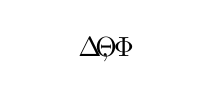
\begin{tikzpicture}[
				sibling distance=30pt, level distance=60pt, 
				t/.style={text height=1.5ex, text depth=.25ex, rectangle, outer sep=0pt}]
			\Tree
				[
					\edge[unary] node[left, midway] {\dep{d}};	
						[\edge[roof, dashed]; \node[t] {\hphantom{123}$\Delta,\Phi$\hphantom{123}};]
					\edge[unary] node[yshift={-7pt}, xshift={11pt}] {\dep{x}}; \node[t,xshift=0pt] {$\Theta$};
				]
			\end{tikzpicture}
			&
			\raisebox{60pt}{$\xleftarrow{\Extraction}$}
			&
			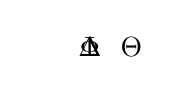
\begin{tikzpicture}[
				sibling distance=7.5pt, level distance=40pt, 
				t/.style={text height=1.5ex, text depth=.25ex, rectangle, outer sep=0pt}, node distance=10pt]
			\tikzset{level 1/.style={level distance=33pt}}
			\tikzset{level 2/.style={level distance=47pt}}
			\tikzset{frontier/.style={distance from root=120pt}}
			\Tree
				[
					\edge node[midway, right] {\dep{d}}; 
					[
						[
							\edge[roof, dashed]; \node[t] {\hphantom{123}$\Delta$\hphantom{123}};
						]
						\edge[unary] node[midway, right] {\dep{x}}; \node[t, xshift={15pt}] {$\Theta$};
						[
							\edge[roof, dashed]; \node[t] {\hphantom{123}$\Phi$\hphantom{123}};
						]
					]
				]
			\end{tikzpicture}
		\end{tabularx}
		\caption{Corresponding tree transformation.}
		\label{subfigure:extraction_tree}
	\end{subfigure}
	\caption{Controlled extraction in the dependency-bracketed setting.}
	\label{figure:modal_dep_extraction}
\end{figure}

Naively, we would assume that the absence of binary bracketing structure in $\LC$ would allow us direct access to the gap within the relative clause body, counteracting the need for the control modalities of (\ref{equation:objrel}).
But the gap is still enclosed, except this time under layers of impenetrable dependency domains!
Seems like we need to reinstate control -- both kinds of modalities must be employed in tandem;
although in truth, the two do not really constitute distinct kinds \textit{per se}: they only differ insofar as their linguistic purposes do.
Nevertheless, it might be handy to make a notational distinction between them, just for the sake of reading comprehension.
From now on, we will use filled symbols to denote control modalities (i.e. ones whose purposes are confined to rebracketing and movement), and white symbols to denote dependency modalities (i.e. ones whose purpose is linguistic annotation, and the brackets of which we expect to see in the antecedent of the proof's end yield).
Even when having a single control pair, assigning it an explicit label \dep{x} is still useful, since it will allow us to tell its brackets apart from the rest.
In this regime, our relativizer's type assignment becomes:
\begin{equation}
\text{that} :: \subcat{l}{rel}{o} := \dbox{mod}(\np\divleft\np)\divright\ddia{body}(\s\divright\dxdia{x}\dxbox{x}\ddia{obj}\np)
\end{equation}
which is faithful to both (\ref{equation:deprel}) and (\ref{equation:objrel}), as it conveys that the missing object is now \textit{movable}.


\begin{figure}
	\[
	\resizebox{1\textwidth}{!}{
		\infer[\divright E]{\w{that}, \dbra{\dbra{\dbra{\w{the}}{det}, \w{eye}}{su}, \w{may}, \dbra{\dbra{\w{never}}{mod}, \w{behold}}{vc}}{body} \vdash \dbox{mod}(\np\divleft\np)}{
			\infer[\Lex]{\w{that} :  \subcat{l}{rel}{o}}{}
			&
			\hspace{-50pt}
			\infer[\ddia{body}I]{\dbra{\dbra{\dbra{\w{the}}{det}, \w{eye}}{su}, \w{may}, \dbra{\dbra{\w{never}}{mod}, \w{behold}}{vc}}{body} \vdash \ddia{body}(\s\divright\ddia{obj}\np)}{
				\infer[\divright I]{\dbra{\dbra{\w{the}}{det}, \w{eye}}{su}, \w{may}, \dbra{\dbra{\w{never}}{mod}, \w{behold}}{vc} \vdash \s\divright\ddia{obj}\np}{
					\infer[\dxdia{x}E]{\dbra{\dbra{\w{the}}{det}, \w{eye}}{su}, \w{may}, \dbra{\dbra{\w{never}}{mod}, \w{behold}}{vc}, \varj \vdash \s}{
						\infer[\divleft E]{\dbra{\dbra{\w{the}}{det}, \w{eye}}{su}, \w{may}, \dbra{\dbra{\w{never}}{mod}, \w{behold}}{vc}, \dbra{\vari}{x} \vdash \s}{
							\infer*{\dbra{\dbra{\w{the}}{det}, \w{eye}}{su} \vdash \ddia{su}\np}{	}
							&
							\infer[\divright E]{\w{may}, \dbra{\dbra{\w{never}}{mod}, \w{behold}}{vc}, \dbra{\vari}{x} \vdash \gtype{itv}}{
								\infer[\Lex]{\w{may} : \gtype{aux}}{}
								&
								\hspace{-25pt}\infer[\Extraction]{\dbra{\dbra{\w{never}}{mod}, \w{behold}}{vc}, \dbra{\vari}{x} \vdash \ddia{vc}\gtype{itv}}{
									\infer[\ddia{vc}I]{\dbra{\dbra{\w{never}}{mod}, \w{behold}, \dbra{\vari}{x}}{vc} \vdash \ddia{vc}\gtype{itv}}{
										\infer[\divright E]{\dbra{\w{never}}{mod}, \dbra{\vari}{x} \vdash \gtype{itv}}{
											\infer[\dbox{mod}E]{\dbra{\w{never}}{mod} \vdash \gtype{itv}\divright\gtype{itv}}{
												\infer[\Lex]{\w{never} : \gtype[l]{adv}_{\divright}}{}
											}
											&
											\infer[\divright E]{\w{behold}, \dbra{\vari}{x} \vdash \gtype{itv}}{
												\infer[\Lex]{\w{behold}: \gtype[l]{tv}}{}
												&
												\infer[\dxbox{x} E]{\dbra{\vari}{x} \vdash \ddia{obj} \np}{
													\infer[\Ax]{\vari : \dxbox{x}\ddia{obj}\np}{}
												}
											}
										}
									}
								}
							}
						}
						&
						\hspace{-60pt}
						\infer[\Ax]{\varj : \dxdia{x}\dxbox{x}\ddia{obj}\np}{}
					}
				}
			}
		}
	}
	\]
	\caption{Dependency-enhanced adaptation of the proof of Figure~\ref{subfigure:lovecraft_rel_clause:rc}, exemplifying the interaction between dependency and control modalities.}
	\label{figure:lovecraft_dep_rep_clause}
\end{figure}


Mobility, however, also means something different now.
Taking inspiration from the established structural vocabulary (see Figure~\ref{figure:modal_structural_rules} if you need to jog your memory), we need to concoct a novel structural rule: one that allows the \textit{extraction} of a nested substructure under the appropriate bracketing conditions.
The magical conconction is presented in Figure~\ref{subfigure:extraction_rule}.
Within arbitrary context $\Gamma$, it looks for a \dep{d}-labelled unary tree enclosing a \dep{x}-labelled unary tree $\Theta$ wrapped by sequences $\Delta$ to the left and $\Phi$ to the right.
There, it allows us to pull the $\Delta$ out, casting the outermost unary tree into a binary sequence and assigning \dep{d} to the concatenation of $\Delta$ and $\Phi$ alone. 
If this makes little sense, see Figure~\ref{subfigure:extraction_tree} for a visual rendition.
\hide{If still unclear, move your mental cursor four sentences back (this one included) and try again.}

Equipped with this missing bit of \hide{alchemical }knowledge, we're at long last able to produce analyses for some less contrived linguistic examples; Figure~\ref{figure:lovecraft_dep_rep_clause} presents the dependency-enhanced derivation we set out to deliver.
Before we move on, though, some important observations are in order.
First, the presentation makes an implicit quantification over the outer label, \dep{d} -- if we were to be really pedantic, we'd need a unique instantiation of that rule for each dependency (but not control!) modal label in the logic.
Beyond a bookkeeping obligation, this parameterization can also be to our advantage: it allows us to directly control which of the dependency domains allow extraction, and which do not.
On a less bureaucratic note, the contextual formulation of the rule carries the usual problem of complicating syntactic equality checking. 
In practice, we can employ a localized version, i.e. one where $\Gamma$ is a flat context (i.e. a sequence with a hole), which means that extractions need to be preemptively applied before every bracketing operation, rather than deferred and done in bulk in the future.
Finally, it is important to remember that the rule is supplementary to (and \textit{not} a substitute for) controlled associacitivity and/or commutativity: altering the linear order of substructures in $\logic{(N)L}$ and/or their binary brackets in $\NL$ still calls for different structural rules with possibly different control modalities that will need to coexist with the \Extraction{} rule for structures to find their intended positions.


\paragraph{Ever higher order}
The example just inspected hides a crucial wisdom: variable abstraction applies to variables -- \textit{not} complex structures thereof.
Control modalities may impose transient bracketing structure upon hypotheses, temporarily hindering their abstraction, but it is always retroactively redacted with the $\diamond E$ rule (after all the necessary structural operations have taken effect).
The bracketing imposed by dependency modalities, however, is built to last, posing a potential roadblock to hypothetical reasoning and higher-order types.

Hypothetical complements are relatively easy to tackle: they just come packed with their diamonds at variable instantiation time.
Excluding the presence of the irrelevant control box, this is exactly the strategy followed in the example under scrutiny (see the $\Ax$ rule instantiating $\vari$ in Figure~\ref{figure:lovecraft_dep_rep_clause}).
Upon closer inspection, we can verify that this is in fact just the $\eta$ normalized version of hypothesizing a plain type, assigning it the desired dependency brackets via the $\diamond I$ rule, and then performing a substitution of the bracketed variable for a logical equivalent (wrapped under the necessary control brackets) via the $\diamond E$ rule -- consult Figure~\ref{figure:eta_normalized_complement_hypothesis} and contrast with Figure~\ref{figure:modal_eta_reductions} if unconvinced.

\begin{figure}
	\begin{tabularx}{0.9\textwidth}{@{}cCc@{}}
	$
		\infer[\ddia{obj} E]{\dbra{\vari}{x} \vdash \ddia{obj}\np}{
			\infer[\ddia{obj} I]{\dbra{\vark}{obj} \vdash \ddia{obj}\np}{
				\infer[\Ax]{\vark : \np}{}
			}
			&
			\infer[\dxbox{x} E]{\dbra{\vari}{x} \vdash \ddia{obj}\np}{
				\infer[\Ax]{\vari : \dxbox{x}\ddia{obj}\np}{}
			}
		}
	$
	&
	\raisebox{10pt}{$\overset{\eta}{\equiv}$}
	&
	$
		\infer[\dxbox{x} E]{\dbra{\vari}{x} \vdash \ddia{obj} \np}{\infer[\Ax]{\vari : \dxbox{x}\ddia{obj}\np}{}}
	$
	\end{tabularx}
	\caption{$\eta$ long form of the $\ddia{obj}$ connective of hypothesis $\vari$  in Figure~\ref{figure:lovecraft_dep_rep_clause}.}
	\label{figure:eta_normalized_complement_hypothesis}
\end{figure}

Hypothetical adjuncts are less forgiving.
A hypothesized adjunct will seek to apply itself to some phrasal head, which is impossible unless it first drops its box.
But in dropping its box, it becomes enclosed in structural dependency brackets that prohibit its eventual abstraction.
We will need to once more resort to the $\diamond E$ rule to remove it, except this time it will be the interior combination of Figure~\ref{subfigure:modal_properties:interior} that we are invoking, which is not subject to $\eta$ contraction.
To see this in action, let us once more consider an excerpt from our go-to source: \textex{a city of high walls where sterile twilight reigned}%
\footnote{H.P. Lovecraft, \textit{Azathoth} (1938). In \textit{Leaves} (2).}.
The relative adverb \textex{where} heads yet another a relative clause, \textex{where sterile twilight reigned}, acting as a postnominal modifier to the noun phrase \textex{a city of high walls}.
The relative clause differs to the ones so far inspected, in missing from its embedded subordinate \textex{sterile twilight reigned \gap} not a complement, but an adjunct: a gap-equivalent to the lexical \textex{there} of Figure~\ref{subfigure:opiate_oceans_poured_there}, except dependency-enhanced, i.e. $\dbox{mod}(\smallgtype{itv}\divleft\smallgtype{itv})$ in shorthand.
As Figure~\ref{subfigure:higher_order_dep:erasure} illustrates, the need for bracket erasure necessitates prefixing the gap type with a residual diamond, steering us towards our first ever fourth order type:
\begin{equation}
\text{where} :: \subcat{l}{rel}{loc} := \dbox{mod}(\np\divleft\np)\divright\ddia{body}(\s\divright(\ddia{mod}\dbox{mod}(\smallgtype{itv}\divleft\smallgtype{itv}))
\end{equation} 
This beast of a type plays the starring role in the derivation of Figure~\ref{figure:higher_order_dep}; it promises to provide a postnominal modifier, if presented with a (third order) relative clause body, that being a sentence missing to its right a diamond-marked (second order) postverbal modifier.

\begin{figure}
	\begin{subfigure}{1\textwidth}
		\smaller
		\[
			\infer[\divleft E]{\w{reigned}, \varj \vdash \gtype{itv}}{
				\infer[\Lex]{\w{reigned} : \gtype{itv}}{}
				&
				\infer[\ddia{mod}E]{\varj \vdash \gtype{itv}\divleft\gtype{itv}}{
					\infer[\dbox{mod}E]{\dbra{\vari}{mod} \vdash \gtype{itv}\divleft\gtype{itv}}{
						\infer[\Ax]{\vari : \dbox{mod}(\gtype{itv}\divleft\gtype{itv})}{}
					}
					&
					\infer[\Ax]{\varj : \ddia{mod}\dbox{mod}(\gtype{itv}\divleft\gtype{itv})}{}
				}
			}
		\]
		\caption{Structurally freeing a hypothesized adjunct...}	
		\label{subfigure:higher_order_dep:erasure}
	\end{subfigure}\\[\midsep]
	\begin{subfigure}{1\textwidth}
		\smaller
		\[
			\infer[\!\divright E]{\w{where}, \dbra{\dbra{\dbra{\w{sterile}}{mod}, \w{twilight}}{su}, \w{reigned}}{body} \vdash \dbox{mod}(\np\divleft\np)}{
 				\infer[\!\!\Lex]{\w{where} : \subcat{l}{rel}{loc}}{}
				&
				\hspace{-5pt}
				\infer[\!\!\ddia{body}I]{\dbra{\dbra{\dbra{\w{sterile}}{mod}, \w{twilight}}{su}, \w{reigned}}{body} \vdash \ddia{body}(\s\divright(\ddia{mod}\dbox{mod}(\gtype{itv}\divleft\gtype{itv})))}{
					\infer[\divright I]{\dbra{\dbra{\w{sterile}}{mod}, \w{twilight}}{su}, \w{reigned} \vdash \s\divright(\ddia{mod}\dbox{mod}(\gtype{itv}\divleft\gtype{itv}))}{
						\infer[\divleft E]{\dbra{\dbra{\w{sterile}}{mod}, \w{twilight}}{su}, \w{reigned}, \varj \vdash \s}{
							\infer[\ddia{su}I]{\dbra{\dbra{\w{sterile}}{mod}, \w{twilight}}{su} \vdash \ddia{su}\np}{
								\infer[\divright E]{\dbra{\w{sterile}}{mod}, \w{twilight} \vdash \np}{
									\infer[\dbox{mod}E]{\dbra{\w{sterile}}{mod} \vdash \np\divright\np}{
										\infer[\Lex]{\w{sterile} : \gtype{adj}_{\divright}}{}
									}
									&
									\infer[\Lex]{\w{twilight}: \np}{}
								}
							}
							&
							\infer{\w{reigned}, \varj \vdash \gtype{itv}}{\text{(\ref{subfigure:higher_order_dep:erasure})}}
						}
					}
				}
			}
		\]
		\caption{...to provide a gap in the higher-order argument of the relative adverb \textex{where}.}
		\label{subfigure:higher_order_dep:rc}
	\end{subfigure}
	\caption{Deriving a locative relative clause.}
	\label{figure:higher_order_dep}
\end{figure}

But why go through all this trouble of producing the dependency brackets only to then immediately cancel them out?
The alternative of hypothesizing a plain functor without any dependency markings would be logically valid but grammatically suboptimal and contrary to our agenda, as it would give us no insights on what the dependency function of the gap is -- the modalities stay.
Another, more pressing question is that of the compatibility between hypothetical adjuncts and the control modality of the previous paragraph, i.e. how could we deal with the nested gap in e.g. \textex{where sterile twilight \textbf{may} reign \gap}.
Fortunately, we need not worry: our previous treatment still holds with only the most minor of adjustments.
Same as before, we have to alter the typing of the gap by prepending a boundary crossing permit, the interior pair $\dxdia{x}\dxbox{x}$.
As the modal chains are no longer $\eta$ contractable, the gap will manifest as three distinct variables, sequentially substituting one for another via two $\diamond E$ rules, as shown in Figure~\ref{figure:higher_order_nested_dep}.
The first substitution of $\vari$ for $\varj$ is responsible for removing the \dep{mod} brackets for \dep{x} ones, allowing any applications of the \Extraction{} rule in the telescoped subproof $s$.
The bracketed variable will eventually be positioned at the outermost branch of the antecedent tree, at which point it can be substituted for $\vark$, the ``true'' variable of the gap.
Don't give in to despair; this is peak complexity -- with these type patterns at our disposal we should be able to tackle any linguistic phenomenon we might encounter from this point on.
Note, finally, that complement and adjunct gaps are not that different to one another after all: they both mimic their corresponding lexical assignment (a plain type or a boxed functor, respectively), except prepended by a diamond of whichever dependency role they will assume and (if needed) a structural extraction licensor.


\begin{figure}
	\smaller
	\[
		\infer{\vdots}{
			\infer[\dxdia{x} E]{\dbra{\Gamma}{d}, \vark \vdash \prop{A}}{
				\infer*[s]{\dbra{\Gamma}{d}, \dbra{\varj}{x} \vdash \prop{A}}{
					\infer[\ddia{mod} E]{\dbra{\varj}{x} \vdash \gtype{itv}\divleft\gtype{itv}}{
						\infer[\dbox{mod} E]{\dbra{\vari}{mod} \vdash \gtype{itv}\divleft\gtype{itv}}{
							\infer[\Ax]{\vari : \dbox{mod}(\gtype{itv}\divleft\gtype{itv})}{}
						}
						&
						\infer[\dxbox{x} E]{\dbra{\varj}{x} \vdash \ddia{mod}\dbox{mod}(\gtype{itv}\divleft\gtype{itv})}{
							\infer[\Ax]{\varj : \dxbox{x}\ddia{mod}\dbox{mod}(\gtype{itv}\divleft\gtype{itv})}{}
						}
					}
				}
				&
				\hspace{-40pt}
				\infer[\Ax]{\vark : \dxdia{x}\dxbox{x}\ddia{mod}\dbox{mod}(\gtype{itv}\divleft\gtype{itv})}{}
			}
		}
	\]
	\caption{Schematic pattern for extracting a nested hypothetical adjunct.}
	\label{figure:higher_order_nested_dep}
\end{figure}

\subsection{Interfaces}
Having completed our tour of dependency-decorated proofs, it is time for respite and reflection.
Let us take a moment to internalize where we started from and where we are now.

\subsubsection{Dependency Trees}
\label{subsubsection:dependency_trees}
Our first ambition was to provide categorial type logics with the means necessary to argue about dependency relations, ideally subsuming dependency trees within the logic's antecedent structures. 
To claim our endeavour a success, we need to actually \textit{show} how these dependency trees can be extracted.

Let's begin with some trivial observations.
In the domain of dependency annotated proofs, endsequents will contain neither variables nor any control brackets.
Collapsing any notion of structure imposed by the functional core (i.e. drop constituency and word order from the builtin structural binder, since dependency trees are agnostic to those), we end up with structures made exclusively of constants (terminal nodes), multisets of structures (unordered variadic branches) and dependency-enclosed structures (unary branches).
This typological description can be further refined by noticing that the non-zeroary tree operators alternate in turns: there's no chaining of unary brackets (each phrase is only assigned at most one dependency role), nor a multiset of multisets (as the simplified structural binder is flat).
Finally, consider that each multiset will coincide with a dependency domain, containing exactly one (unmarked) head constant (necessarily a word), some $n$ adjuncts and some $m$ complements.

With these in mind, we arrive at the following (modulo permutation) inductive definition of a dependency induced structure:
\begin{equation}
	\Gamma
		 	:=  
 	\underbrace{\dbra{\Gamma_0}{d_0} \dots \dbra{\Gamma_{n-1}}{d_{n-1}}}_{\text{adjuncts}} \ 
	\underbrace{\dbra{\Gamma_n}{d_n} \dots \dbra{\Gamma_{n + m - 1}}{d_{n + m -1}}}_{\text{complements}} \ 
	\underbrace{\vphantom{\Gamma_0^a}\kappa}_{\text{head}} \
\end{equation}
Converting such a structure to a dependency tree akin to the one of Figure~\ref{figure:udparse} is pleasantly easy: just apply the function below to it (plug an invisible ``root'' node and label to get things going).%
\footnote{For the more verbally inclined, we need to simply enter every dependency domain and establish an arc from the local head to (the head of) each of its dependents.}
\begin{align*}
& \mathsf{deptree :: Struct \to Head \to \deps \to Set[Arc]}\\
& \mathsf{deptree} \ 
			\left(\dbra{\Gamma_0}{d_0} \dots \dbra{\Gamma_{n + m - 1}}{d_{n + m -1}} \ 
			\kappa\right)
			\ 
			\mathsf{root}
			\ 
			\mathsf{label} = \\
& \quad	
			 \{ \mathsf{root} \xrightarrow{\mathsf{label}} \kappa \}
			\cup \raisebox{0pt}[0pt]{$\bigcup\limits_{i=0}^{n+m-1}$}\{\mathsf{deptree} \ \Gamma_i \ \ \kappa \ \ d_i\}
\end{align*}
Figure~\ref{figure:example_deps} shows the function's yield applied to two of the section's example derivations.
Given a partition of $\deps$ into adjuncts and complements, the conversion can trivially be extended with the bidirectional dependency arcs described in Section~\ref{subsection:dep_grammars}.
Word order is also straightforward to capture, if we just keep the structural order provided by a non-commutative calculus intact.
In any case, our efforts go to show that the general structure of a dependency tree can easily be captured by a dependency-enhanced type logic using the type assignment patterns discussed.
Aligning the type logic to a specific flavour of a dependency grammar was never our main intention, but should be fairly easy to accomplish by reverse-engineering the annotational specifics of the target: a task for future generations.

\begin{figure}
	\centering
	\begin{subfigure}{1\textwidth}
		\centering
		\begin{tikzpicture}[t/.style={text height=1.5ex, text depth=.25ex, rectangle, outer sep=0pt}, node distance=10pt]
		\smaller
		\node[t] (that)		at (0,0) {\w{that}};
		\node[t] (the)		[right=10pt of that] {\w{the}};
		\node[t] (eye)		[right=10pt of the] {\w{eye}};
		\node[t] (may)		[right=10pt of eye] {\w{may}};
		\node[t] (never)	[right=10pt of may] {\w{never}};
		\node[t] (behold)	[right=10pt of never] {\w{behold}};
		\path[->] (that) [bend left=75] edge node [above] {\smaller[2]{body}} (may);
		\path[->] (may) [bend right=50] edge node [above] {\smaller[2]{su}} (eye);
		\path[->] (eye) [bend right=50] edge node [above] {\smaller[2]{det}} (the);
		\path[->] (may) [bend left=70] edge node [above] {\smaller[2]{vc}} (behold);
		\path[->] (behold) [bend right=40] edge node [above] {\smaller[2]{mod}} (never);
		\end{tikzpicture}
		\caption{Dependency tree of $\ctx{\w{that}, \dbra{\dbra{\dbra{\w{the}}{det}, \w{eye}}{su}, \w{may}, \dbra{\dbra{\w{never}}{mod}, \w{behold}}{vc}}{body}}$.}
		\label{subfigure:that_the_eye_may_never_behold_deps}
	\end{subfigure}\\[\midsep]
	\begin{subfigure}{1\textwidth}
	\centering
		\begin{tikzpicture}[t/.style={text height=1.5ex, text depth=.25ex, rectangle, outer sep=0pt}, node distance=10pt]
		\smaller
		\node[t] (where)		at (0,0) {\w{where}};
		\node[t] (sterile)		[right=10pt of where] {\w{sterile}};
		\node[t] (twilight)		[right=10pt of sterile] {\w{twilight}};
		\node[t] (reigned)		[right=10pt of twilight] {\w{reigned}};
		\path[->] (where) [bend left=55] edge node [above] {\smaller[2]{body}} (reigned);
		\path[->] (reigned) [bend right=40] edge node [above] {\smaller[2]{su}} (twilight);
		\path[->] (twilight) [bend right=40] edge node [above] {\smaller[2]{mod}} (sterile);
		\end{tikzpicture}
		\caption{Dependency tree of $\ctx{\w{where}, \dbra{\dbra{\dbra{\w{sterile}}{mod}, \w{twilight}}{su}, \w{reigned}}{body}}$.}
		\label{subfigure:where_sterile_twilight_reigned_deps}
	\end{subfigure}
	\caption{Trees extracted from the derivations of Figures~\ref{figure:lovecraft_dep_rep_clause} (\subref{subfigure:that_the_eye_may_never_behold_deps}) and~\ref{figure:higher_order_dep} (\subref{subfigure:where_sterile_twilight_reigned_deps}).}
	\label{figure:example_deps}
\end{figure}

\subsubsection{Semantics}
The trees of Figure~\ref{figure:example_deps} leave something to be desired: by backpedaling towards dependency grammars, higher-order phenomena have been completely dismissed -- wasted are all our efforts to tame and manage the bracketing structures of hypotheses.
Perhaps importing residuated modalities just for the sake of cracking some dull and flat dependency relations was an overkill after all?
The answer is no.
Antecedent bracketing structures is but the most superficial aspect of our grammar logic's proofs -- the function argument relations of the implicational core are retained, and in fact coexist with the dependency annotations (including higher-order ones) in the logic's term calculus, which we have been unjustly ignoring.

The far richer type and term structure of the syntactic calculus creates, in turn, ample opportunity for the passage to semantics.
We are of course still presented with the cautious option of simply forgetting about dependencies, retracting to the same dependency agnostic $\ILL$ we did earlier.
But the radical path would have us preserve dependency operators in the intermediate station of derivational semantics%
	\footnote{And thus necessarily also the extraction pair $\dxdia{x}$, $\dxbox{x}$.},
in hope of them findind downstream applications later on.
A first merit would be the availability of richer type assignments in the lexical semantics domain, where previously identical function types become distinguishable by virtue of their modal decorations.
There, syntactic modalities can be translated to semantic operators, lifting the target signature accordingly and allowing for a stronger syntax-semantics interface -- as for what these translations might be, quite a few reasonable paths are presented.
\textit{Monads} make for a natural translation choice, both because of their affinity with modalities~\cite{kobayashi1997monad,corfield2020modal} as well as their progressively maturing adoption by the linguistics community~\cite{asudeh2020enriched}.
Furthermore, dependents are delineated and identified by their syntactic roles, allowing distinct semantic treatments, if so desired.
Even in the modest setting of a non-inflated translation, modalities can help tell which of the (possibly many) combinations of semantic slots are occupied in a given construction, allowing the correct compositional recipe to be retrieved from the semantic lexicon, while still distinguishing between optional and necessary ones~\cite{asudeh2012flexible}.
In the edge case, they open the possibility for a homomorphic translation that ``forgets'' parts of the implicational directives of the logic, relying instead on the source dependency markings for the construction of its semantic terms.


\section{Key References \& Further Reading}
\label{section:references_2}
The chapter has presented novel work, assembled and expanded from streamlined bits and pieces of earlier published drafts.
The good news is you're reading the most extensive overview available at the time of writing.
The bad news is I don't have much references for you -- if it's any consolation, there's still two more chapters to go.
Of work not included in this chapter or the ones to come, the one by \citet{rouss} has dependency modalities play a key role in the annotation and generation of complex verb clusters with subtle semantic dependencies, the recursive nature of which seems to break the omnipotence attributed to neural language models.
For a less avant-garde reading, I'd like to draw your attention to this chapter's historical roots, namely the manuscript of \citet{moortgat1991heads}.
If unsated and craving for more modalities-as-dependencies, you have the option of either writing something yourself or waiting until someone else does.\footnote{Calling it now, next big development in Moortgat et al. [2051].}

More broadly and outside their use as dependency markers, unary modalities have long now been a tempting way to encode linguistic features -- see \citet{moa} and \citet{10.7551/mitpress/6169.003.0012,johnson1999resource}, for instance.
Further away from our niche territories, the relation between dependency grammars and lexicalism is extensively analyzed by \citet{kuhlmann2010dependency}, who asks (and answers) the question of which formal grammars induce what kind of dependency structures.
On a relevant note, the slightly disheveled categorial dependency grammars make for an attempt to provide a categorial treatment of dependency structure, where the arcs and their labels are in themselves the grammar's base types~\cite{dekhtyar2015categorial}.

\bibliographystyle{abbrvnat}
\bibliography{bibliography}
\chapter{Proof Extraction}
\label{chapter:chapter_3}

\chapabstract{\textit{What good is a program that only lives on paper?}}

With our theorycrafting over, we have in our hands an uninstantiated descriptive model of syntactic and semantic composition, promising to capture dependency relations while keeping both its feet set firmly in type theory.
Unfortunately, it is well attested by now that ``all models are wrong...''~\cite{doi:10.1080/01621459.1976.10480949}.
Any promise of theoretical universality, cognitive plausibility, linguistic intrinsicness or what have you, would require some degree of handwaving and conjencturing that I am not comfortable with.
What is undisputable, however, is the nobility of our goals and the purity of our tools: the \textit{omniversality} of the $\lambda$ calculus~\cite{wadler2015propositions} asserts that our modeling approach is not some ad hoc machinery designed to tackle a highly localized problem, but the one and only programming language ever worth writing. 
Beyond purpose and methodology, and having \textit{a priori} given up any ideation of truth, the only measure of success for our model is that of its utility (``...but some are useful'', ~\cite{doi:10.1080/01621459.1976.10480949}).
This sets up a new research imperative: we must prove the model useful!

``Oof, that's a tricky one'', you might say, and you wouldn't be wrong.
Thankfully, there are two tried and tested ways to proceed.
The first is the way of the scholar, which requires a rare combination of high intellectual capacity, strong persuasive skills and a pinch of luck.
It starts off with some profound abstract thinking, gradually overtaken by agressive campaigning: bashing the competition at workshops and conferences, making bold claims and generating traction at any chance given (optionally over social media platforms, for the modernists), eventually building a cult of personality, and finally resting on your laurels as the hype becomes self-sustainining; at long last, utility affirmed by popular approval.
This path, sometimes called the scientific method, is a rather involved and painstakingly slow process, a high stakes gamble that only starts yielding profits in the long run; as such, it greatly benefits from the nourishment of a stable work environment.
More befitting the modern paradigm of the mobile, adaptive, multi-purpose researcher is the alternative path, the way of the engineer.
A shorter term investment, it requires only the acquirable skills of endurance and hardheadedness, and offers a recipe that's easier to follow: simply swing at it until it cracks.
After a lot of obsessive iteration and self-correction (interchanged with the occasional feeling of despair), (f)utility will sooner or later be affirmed by cold, hard numbers.
We'll go for this one.

This choice has some methodological repercussions.
Under more tranquil circumstances, we'd wait for the theory to be disseminated, criticized, adapted, error-corrected and returned to sender, before finally moving on; it being a theory of language, this would entail a thorough qualitative analysis of several kinds of linguistic phenomena, coupled with a theoretical investigation of what it can or cannot adequately capture.
We are however in a compressed timeframe, forcing our hand into putting it straight to the test; the pragmatic approach is then to try and directly align it with real-world linguistic data at scale, and hope for the best.
The process, called \textit{proof extraction}, revolves around ``proving''  some source corpus of syntactically annotated sentences via the design and application of an algorithm tasked with translating the existing annotation format into derivations of the target grammar.
Proof extraction serves a ternary purpose.
One, it gives us access to an uncompromisingly realistic testbed upon which we can immediately inspect and iteratively finetune the specifics of the grammar logic.
Two, it fills in for a strict and impartial external critic in providing a quantitative evaluation regime -- at each point in time, we are able to measure the proportion of source analyses (and corresponding linguistic phenomena) the algorithm provides a (reasonable) output for.
And three, the end-yield of this process has merit of its own.
As a derived dataset, it is first a building block necessary for populating the computational toolshed of the theory, and also a public resource for the world to with as they please.

\section{Preliminaries}

\subsection{The Dutch Language}
For our linguistic inquiries, the focus will be on Dutch.
Other than being the language I was contractually obliged to conduct this research on, Dutch is an interesting specimen, the idiosyncracies of which have in the past proven quite a topic of debate for others, and a source of headaches for myself.
I don't have any intention (or delusion of competence) to casually throw a detailed exposition of the Dutch grammar here, but a brief and superficial typological overview might help smooth the transition into the what is to come.
If the section has the opposite effect to the one intended, know that I'll hold no grudge if you skip ahead.

But first things first.
Dutch is a West Germanic language, spoken primarily in the Low Countries within Europe by some 25 million speakers.
Owing to the Netherlands' nasty colonial history, Dutch has left a noticeable mark on the global linguistic atlas: it has played a primary role in the evolution of Afrikaans and, to a far lesser extent, Indonesian, while native Dutch speakers can be found as far as South America and the Dutch Carribean region.
Demographics aside, the language is said to be one of the closest relatives of English and German, sharing many of their morphosyntactic characteristics -- we'll go through some of those together.
The abbrevations in the glosses to follow are industry standard, you can find their transcriptions in Table~\ref{table:gloss_abbreviations} of Appendix~\ref{sec:abbrevations}.
Any internal inconsistencies are deliberate: I am trying to gloss only those features relevant to the local discussion.

\subsubsection{The Noun Phrase}
\paragraph{Nouns}
Dutch nouns have three grammatical genders: the masculine, the feminine and the neuter.
The masculine and feminine genders are morphologically indistinguishable -- telling them apart is done on the basis of the lexicon alone.
\begin{exe}
\ex\label{gloss:genders}
\begin{xlist}
\ex
\gll \textit{de} \textit{aard}\\
the earth(\abbrv{m})\\
\ex
\gll \textit{de} \textit{zee}\\
the sea(\abbrv{f})\\
\ex
\gll \textit{het} \textit{bos}\\
the forest(\abbrv{n})\\
\end{xlist}
\end{exe}
There's two numbers, the singular and the plural, the latter constructed with the aid of the suffix \textex{-en} or rarely \textex{-s}, depending on the noun.
\begin{exe}
\ex 
\begin{xlist}
\ex
\gll \textit{de} \textit{zeven} \textit{zee-\"{e}n}\\
the seven sea-\abbrv{pl}\\
\glt{`the seven seas'}
\ex
\gll \textit{de} \textit{trekvogel-s}\\
the  migratory.bird-\abbrv{pl}\\
\glt{`the migratory birds'}
\end{xlist}
\end{exe}
Case markings are not overtly realized, except for some mostly frozen leftovers from the distant past -- their functionality has largely been replaced by word order constraints, with the indirect object (formerly in the dative) preceding the direct object (formerly in the accusative), and periphrastic constructions, with the preposition \texttr{aan}{to} used to indicate indirect objects (see Gloss~\ref{gloss:ido} later on), and \texttr{van}{of} to substitute the genitive.
\begin{exe}
\ex
\gll \textit{het} \textit{oog} \textit{van} \textit{de} \textit{geest}\\
the eye of the mind\\
\glt{`the mind's eye'}
\end{exe}
A cute peculiarity of Dutch is the strikingly common use of a productive diminutive form, denoting either small size or an affectionate disposition -- diminutives are formed with the suffix \textex{-tje} or regionally \textex{-ke}, and are always neuter (notice the gender change of Gloss~\ref{gloss:gender_change}).

\paragraph{Determiners}
Determiners precede the noun and match its gender and number.
There are two articles: the definite, and the indefinite.
The definite has two singular forms \textex{de}/\textex{het} (non-neuter/neuter) and a single plural \textex{de}. 
Non-neuter forms are used for both masculine and feminine (refer back to Gloss~\ref{gloss:genders}).
\begin{exe}
\ex\label{gloss:gender_change}
\begin{xlist}
\ex
\gll de klein-e vogel\\
the(\abbrv{nn.sg}) small-\abbrv{def} bird\\
\glt{`the small bird'}
\ex
\gll het klein-e vogel-tje\\
the(\abbrv{n.sg}) small-\abbrv{def} bird-\abbrv{dim}\\
\glt{`the small birdie'}
\end{xlist}
\end{exe}
The indefinite \textex{een} is gender-agnostic, and has no plural form.
\begin{exe}
\ex
\begin{xlist}
\ex\label{gloss:indef_adj_sg_n}
\gll een donker lied\\
a dark song\\
\glt{`a dark song'}
\ex 
\gll donker-e lied-eren\\
dark-\abbrv{pl} song-\abbrv{pl}\\
\glt{`dark songs'}
\end{xlist}
\end{exe}
Indefinite pronouns can be used to convey universal or existential quantification and negation, materializing as substitutes for determiners (e.g. \texttr{alles}{all}, \texttr{sommige}{some}, \texttr{geen}{no}, etc.), or as stand-alones (e.g. \texttr{iets}{something}, \texttr{niets}{nothing}, etc.).
\begin{exe}
\ex
\gll Alle mensen willen iets, sommige willen alles.\\
all people want something some want everything\\
\glt{`All people want something, some want everything.'}
\end{exe}
Possessive and demonstrative pronouns can also enact determiners, both uninflected (except for the first person plural \textex{ons} which inflects like an indefinite adjective, see next paragraph).
\begin{exe}
\ex
\gll De eend is mijn favoriet vogel.\\
the duck is my favorite bird\\
\glt{`The duck is my favorite bird.'}
\ex\label{gloss:ido}
\gll Het bos is onz-e tempel.\\
the forest is our-\abbrv{def} temple\\
\glt{`The forest is our temple.'}
\end{exe}
Demonstrative pronouns come in two major flavours: the proximal \textex{deze/dit} (plural \textex{deze}) and the distal \textex{die/dat} (plural \textex{die}).
The last two do double duty as relative pronouns -- more on that later.
When used to substitute (rather than determine) a noun in a copula, each variant reverts to its neuter singular form.
\begin{exe}
\ex
\begin{xlist}
\ex
\gll Deze bergen zijn hoog.\\
these(\abbrv{pl}) mountains are tall\\
\glt{`These mountains are tall.'}
\ex
\gll Dit zijn mijn bergen.\\
this(\abbrv{n}) are my mountains\\
\glt{'These are my mountains.'}
\end{xlist}
\end{exe}

\paragraph{Adjectives}
Adjectives used as nominal modifiers find their place between the determiner and the head noun.
They appear inflected with an \textex{-e} affix in all cases except for the idefinite use with a neuter singular noun (refer back to Gloss~\ref{gloss:indef_adj_sg_n}, contrast with \ref{gloss:gender_change}).
The same affix applies to nominalized adjectives, which can allow the ommission of a contextually implied noun, or be used independently as an abstract concept or a quantifying property.
\begin{exe}
\ex
\gll dood aan het heilig-e\\
death to the holy-\abbrv{nmlz}\\
\glt{`death to the holy'}
\ex
\gll De zachtmoedig-en zullen niets be\"{e}rven.\\
the meek-\abbrv{nmlz.pl} shall nothing inherit(\abbrv{inf})\\
\glt{`The meek shall inherit nothing.'}
\end{exe}
An alternative inflection with a \textex{-s} affix marks the partitive use, when the adjective modifies an indefinite pronoun.
\begin{exe}
\ex
\gll iets ernstigs-s\\
something grave-\abbrv{ptv}\\
\glt{`something grave'}
\end{exe}
The language provides acccess to a comparative and a superlative form, via the affixes \textex{-er} and \textex{-ste} respectively, or periphrastically with \texttr{meer}{more} and \texttr{meest}{most}.
\begin{exe}
\ex
\gll \textit{het} \textit{donker-ste} \textit{lied}\\
the(\abbrv{n.sg}) dark-\abbrv{sup} song\\
\glt{`the darkest song'}
\end{exe}

\paragraph{Personal Pronouns}
Noun phrases can be substituted by personal pronouns, which in Dutch are morphologically marked for case and gender.
The nominative is used for the subject position, the genitive corresponds to the possessive determiners discussed earlier, and the accussative is used to denote objects.
\begin{exe}
\ex
\gll Ik zie een vreemde man in de spiegel.\\
I(\abbrv{nom}) see a strange man in the mirror\\
\glt{`I see a strange man in the mirror.'}
\ex
\gll Hij merkt mij op.\\
he(\abbrv{nom}) perceives me(\abbrv{acc}) on\\
\glt{`He notices me.'}
\end{exe}
A dative form is sometimes exceptionally used for indirect objects in the third person plural.
Depending on the regional variation, personal pronouns must match the grammatical gender of the noun they refer to, or simply default to the neuter (reserving the masculine and feminine forms for animates).
Third person singulars are also interchangeable with the appropriate demonstratives.
Personal pronouns come in two variants: the stressed (emphatic) and the unstressed (standard).

\subsubsection{The Verb}
\paragraph{Conjugation}
In their citation form, verbs match their infinitival versions, regularly consisting of the verbal stem plus \textex{-en}.
Verbal conjugation patterns distinguish between two grammatical tenses, the non-past and the past, and three moods, the indicative, the subjunctive and the imperative, of which the first two are morpohologically conflated.
Each pattern is parameterized by person and number.
Aspectual flavours, passivization and an explicit future are accessible as productive constructions with modals, the latter being the common culprits of irregular conjugation.

\paragraph{Participles}
Participles exist for both tenses, and have a multitude of uses.
The present participle is formed by affixing \textex{-de}, and is commonly employed as an duration-denoting adjective or adverb, always inflected in the first case, and optionally in the second.
\begin{exe}
\ex
\gll de zweven-de vrouw\\
the levitate-\abbrv{prs.ptcp} woman\\
\glt{`the levitating woman'}
\end{exe}
Rarely, it can be used as a complement to the auxiliary \texttr{zijn}{to be} to produce a kind of present continuous.
Present participles of transitives can attach to the end of their object nouns, appearing as fused compounds.
The past participle is more versatile.
Regular past participles are formed by prefixing \textex{ge-} to the verbal stem (morphophonological terms and conditions may apply) and substituting the infinitival suffix for either \textex{-t}, \textex{-d} or nothing, depending on the stem's last phoneme.
Like the present participle, it can be used as an adjective, denoting now a completed event.
\begin{exe}
\ex
\gll beelden met ge-sloten ogen\\
images with \abbrv{pst.ptcp}-close eyes\\
\glt{`closed eye visuals'}
\end{exe}
Combined with with the modal \texttr{hebben}{to have} (or exceptionally \textex{zijn} for unaccusatives and verbs of movement), it produces the perfect tense.
\begin{exe}
\ex
\end{exe}
Combined with the modals \texttr{worden}{to become} and \texttr{zijn}{to be}, it produces the passive voice and its perfect tense.
%\todo
%\begin{exe}
%\ex
%\gll Ge-zegen-d zijn de on-ge-bog-en\\
%\abbrv{pst.ptcp}-bless-\abbrv{pst.ptcp} are the \abbrv{neg}-\abbrv{pst.ptcp}-bow-\abbrv{nmlz.pl}\\
%\glt{`Blessed are the unbowed.'}
%\end{exe}

\paragraph{Infinitives}
Infinitival forms commonly occur as the verbal complements of a modal, auxiliary or perception verb.
\begin{exe}
\ex
\gll Ik wil slapen.\\
I want sleep(\abbrv{inf})\\
\glt{`I want to sleep.'}
\end{exe}
Depending on the modal, the preposition \texttr{te}{to}, or the discontinuous \texttr{om ... te}{to}, may be either necessary, optionally admissible or completely disallowed -- if one does manifest, it precedes the infinitive.
\begin{exe}
\ex
\gll Ik probeer te schrijven.\\
I try to write(\abbrv{inf})\\
\glt{`I try to write.'}
\end{exe}
The discontinuous variant is only selected for by specific verbs -- it can enclose linguistic material, like the infinitive's object or any adverbs modifying it.
\begin{exe}
\ex
\gll Ik dwing mezelf om wat te schrijven.\\
I force myself \_ something to write(\abbrv{inf})\\
\glt{`I force myself to write something.'}
\end{exe}
An infinitive directly following \textex{aan het} can combine with \textex{zijn} to construct the continuous aspect, in either the present or the past tense.
\begin{exe}
\ex
\gll Ik ben aan het schrijven.\\
I am in the write(\abbrv{inf})\\
\glt{`I am writing.'}
\end{exe}
Infinitives are also often nominalized, the resulting nominals being singular neuters.
\begin{exe}
\ex
\gll Het schrijven is pijnlijk.\\
The write(\abbrv{inf}) is painful\\
\glt{`The writing is painful.'}
\end{exe}

\paragraph{Separable Verbs} 
The verbal lexicon contains several compound items comprised of a preposition and a verbal stem, usually with a compositional meaning.
The stem is separated from its prepositional prefix when the verb heads a matrix clause, in which case the preposition is moved to the end of the clause -- in all other cases, including the finite form in subordinate clauses, the two remain attached.
When inflecting for the perfect, the prefix applies to the stem (i.e. after the preposition).

\subsubsection{The Sentence}
By far the most fun aspect of Dutch is its absolutely wild sentential word order.

\paragraph{Main Clauses}
The main clauses inspected so far emanate a false sense of safety, coming off as SVO at first glance, with participles used for the passive voice and the perfect tense pushed to the right edge of the clause.
The truth is far more sinister -- the verb is placed there only by exception, abiding by the V2 rule that has it appear second for matrix clauses only.
The effect becomes apparent when employing a preverbal adverb -- in Gloss~\ref{gloss:simple_smain_v2}, both the subject and its predicate complement follow the verb in a VSO pattern.

\paragraph{Questions and Imperatives}
When it comes to questions, things look familiar again.
Line in English, wh-questions begin with an interrogative pronoun or adverb (e.g. \texttr{wie}{who}, \texttr{waar}{where}, \texttr{welk}{which}, \texttr{waarom}{why} etc.), which is immediately followed by the conjugated verb (Gloss~\ref{gloss:simple_whq}).
In direct questions without an interrogative, as well as positive imperatives, the verb is placed first (Glosses~\ref{gloss:simple_sv1_q} and \ref{gloss:simple_sv1_imp}).
In negative imperative sentences and impersonal commands, the infinitival is placed last.

\begin{exe}
\ex
\begin{xlist}
\ex\label{gloss:simple_smain}
\gll Frans verkoop-t kaas.\\
Frans sell-\abbrv{prs.3sg} cheese\\
\glt{`Frans sells cheese.'}
\ex\label{gloss:simple_smain_v2}
\gll Morgen verkoop-t Frans kaas.\\
tomorrow sell-\abbrv{prs.3sg} Frans cheese\\
\glt{`Frans will sell cheese tomorrow.'}
\ex\label{gloss:simple_sv1_q}
\gll Verkoop-t Frans kaas?\\
sell-\abbrv{prs.3sg} Frans cheese\\
\glt{`Does Frans sell cheese?'}
\ex\label{gloss:simple_whq}
\gll Wie verkoop-t kaas?\\
who sell-\abbrv{prs.3sg} cheese\\
\glt{`Who sells cheese?'}
\ex\label{gloss:simple_sv1_imp}
\gll Verkoop kaas!\\
sell(\abbrv{imp}) cheese\\
\glt{`Sell cheese!'}
\end{xlist}
\end{exe}


\paragraph{Subordinate Clauses}
Subordinate clauses is where things really get interesting.
Unaffected by the V2 rule, the word order turns out to be SOV; this affects indirect questions, verbal complements and relative clauses alike.
Indirect questions are straightforward -- modulo the word order permutation, they match their direct counterparts.
\begin{exe}
\ex\label{gloss:embedded_q}
\gll Weet je wie kaas verkoopt?\\
know you who cheese sells\\
\glt{`Do you know who sells cheese?'}
\end{exe}
Infinitives in non-nested verbal complements are likewise just pushed to the end of their clause.
\begin{exe}
\ex\label{gloss:simple_vc}
\gll Frans wil koopman worden.\\
Frans wants merchant be(\abbrv{inf})\\
\glt{`Frans wants to be a merchant.'}
\end{exe}
Relative clauses are instigated by relative adverbs and pronouns.
Interestingly, the language does not make an overt distinction between an object- and a subject- relative pronoun; combined with the SOV word order, and the absence of case markings, the effect is that the two relative clause types end up having the exact same surface form when the grammatical gender of the antecedent noun and the non-gap embedded argument are the same -- contrast the two sentences below.
\begin{exe}
\ex\label{gloss:rc_ambiguity}
\begin{xlist}
\ex
\gll het geheim dat een bos verbergt\\
the secret(\abbrv{n}) that a forest(\abbrv{n}) hides\\
\glt{
\begin{enumerate}[topsep=0pt]
	\item `the secret the hides a forest'
	\item `the secret that a forest hides'
\end{enumerate}}
\ex
\gll de kerk die vuur opslokt\\
the church(\abbrv{nn}) that(\abbrv{nn}) vuur(\abbrv{n}) consumes\\
\glt{`the church that fire consumes'}
\end{xlist}
\end{exe}

The SOV order means that the chaining of verbs requiring non-finite complements inadvertently leads to \textit{verb clusters}, i.e. collections of two or more verbs situated within the dependent clause and adjacent to one another.
Verb clusters are marked by their inability to accommodate non-verbal material, and may follow a number of different word orders, which don't necessarily abide by the order of selectional dominance.
The question of which factors influence the grammaticality of word order variations  is a hot potato and a topic of active research for decades -- to make matters worse, these factors tend to differ between regional variations of the language%
	\footnote{As a fun trivia,  out of the 6 possible orderings of 3-verb clusters, 4 to 5 were found admissible by Dutch speakers depending on the construction~\cite{3vc}.}.
What follows are some simplified common observations -- the interested reader should find the thesis of~\citet{augustinus2015complement} a good entry point towards more detailed discussions.

For starters, bare infinitives usually follow their governor -- but: this is not necessarily the case for clusters of 2 verbs where the finite verb is a modal.
The first two  below depict the canonical and ``inverted'' word orders; the third example is ungrammaticaul due to the adjective \textex{naamloos} interrupting the cluster.
\begin{exe}
\ex\label{gloss:rusten_zal}
\begin{xlist}
\ex
\gll ... waar ik naamloos zal rusten\\
.... where I nameless will rest(\abbrv{inf})\\
\ex
\gll ... waar ik naamloos rusten zal\\
... where I nameless rest(\abbrv{inf}) will\\
\glt{`... where I will rest nameless'}
\ex[*]{\textit{... waar ik zal naamloos rusten}}
\end{xlist}
\end{exe}
Past participles used in the formation of the perfect or passive may occur either to the left or the right of the tense auxiliaries \textex{hebben} and \textex{zijn}, leading to either a German- or English- like construction.
\begin{exe}
\ex\label{gloss:green_vs_red}
\begin{xlist}
\ex
\gll ... omdat ik de eend ge-zien heb\\
... because I the duck \abbrv{pst.ptcp}-see have\\
\ex
\gll ... omdat ik de eend heb ge-zien\\
... because I the duck have \abbrv{pst.ptcp}-see\\
\glt{`... because I have seen the duck'}
\end{xlist}
\end{exe}
This gets complicated by the so-called IPP (\textit{Infinitivus Pro Participio}) effect, where a participle that selects for an infinitive changes to an infinitive itself, creating a cluster in the process -- once more, whether this substitution is mandatory, optional or altogether impossible is lexically decided.
\begin{exe}
\ex\label{gloss:ipp}
\begin{xlist}
\ex 
\gll Ik heb de eend ge-zien.\\
I have the duck \abbrv{pst.ptcp}-see\\
\glt{`I have seen the duck.'}
\ex
\gll Ik heb de eend zien vliegen.\\
I have the duck see(\abbrv{inf}) fly(\abbrv{inf})\\
\glt{`I have seen the duck fly.'}
\ex\label{gloss:ipp_tv}
\gll Ik heb de eend een nest zien maken.\\
I have the duck a nest see(\abbrv{inf}) make(\abbrv{inf})\\
\glt{`I have seen the duck make a nest.'}
\end{xlist}
\end{exe}
Next, the infinitival head of a dependent clause may be forced to occur directly after the verb dominating it, if the latter belongs to a closed set of so-called \textit{raising} verbs (i.e. the raiser is infixed between the infinitive to the right, and the infinitive's non-verbal arguments to the left).
These include modals like \texttr{willen}{to want} and \texttr{moeten}{must}, perception verbs like \texttr{horen}{to hear} and \texttr{zien}{to see}, and some nondescript verbs like \texttr{doen}{to do} and \texttr{laten}{to let}.
As before, they can be subcategorized as obligatory raisers and optional ones.
\begin{exe}
\ex
\gll Ik denk dat ik iemand hoor naderen\\
I think that I someone hear approach(\abbrv{inf})\\
\glt{`I think I hear someone approaching.'}
\end{exe}
Yet other verbs like \texttr{verplichten}{to forbid} select not a bare infinitive but a \textex{te}-marked infinitival phrase, which they leave intact at the end of the clause -- a phenomenon known as \textit{extraposition}.
The twist is that the intersection of extraposition verbs and raising verbs is non-empty -- \texttr{proberen}{to try}, for instance, can behave as either.

\goodbreak\begin{exe}
\ex\label{gloss:vr_vs_xpos}
\begin{xlist}
\ex
\gll \textit{Ik} \textit{denk} \textit{dat} \textit{hij} \textit{probeert} \textit{iets} \textit{te} \textit{zeggen}.\\
I think that he tries something to say(\abbrv{inf})\\
\ex
\gll \textit{Ik} \textit{denk} \textit{dat} \textit{hij} \textit{iets} \textit{probeert} \textit{te} \textit{zeggen}.\\
I think that he something tries to say(\abbrv{inf})\\
\glt{`I think that he is trying to say something'}
\end{xlist}
\end{exe}

Typology aside, Dutch verb clusters have been a favorite topic of debate for formal grammarians for a while now, since their construction requires expressive capacity beyond what a context-free grammar can offer, and thus brinking an end to any delusion that human languages are context-free%
	\footnote{Or, depending on the reader, that Dutch is a human language.}%
~\cite[\textit{inter alia}]{huybregts1984weak,shieber1985evidence}.
The impenetrable nature of verb clusters means that verbs that partake in their construction may often be forced to detach from their arguments, or worse yet become stranded from them by the infixation of another verb in between -- in the dependency grammar paradigm, these discontinuities materialize as non-projective (or cross-serial) dependencies -- see Figure~\ref{figure:xdep_udparse} for an example.

\begin{figure}
	\centering
	\begin{tikzpicture}[t/.style={text height=1.5ex, text depth=.25ex, rectangle, outer sep=0pt}, node distance=10pt]
	\smaller
%%	\node[t] (1) 			
	\node[t] (1)			at (0, 0) {\w{ik}};
	\node[t] (2)			[right=10pt of 1] {\w{heb}};
	\node[t] (3)			[right=10pt of 2] {\w{de}};
	\node[t] (4)			[right=10pt of 3] {\w{eend}};	
	\node[t] (5)			[right=10pt of 4] {\w{een}};	
	\node[t] (6)			[right=10pt of 5] {\w{nest}};
	\node[t] (7)			[right=10pt of 6] {\w{zien}};
	\node[t] (8)			[right=10pt of 7] {\w{maken}};
	\draw[->] (2) [bend right=80] edge node [above] {\smaller[2]{nsubj}} (1);
	\draw[->] (2) [bend left=90] edge node [above] {\smaller[2]{vc}} (7);
	\draw[->] (2) [bend left=90] edge node [above] {\smaller[2]{obj}} (4);
	\draw[->] (4) [bend right=60] edge node [above] {\smaller[2]{det}} (3);
	\draw[->] (7) [bend left=70] edge node [above] {\smaller[2]{vc}} (8);
	\draw[->] (8) [bend right=90] edge node [above] {\smaller[2]{obj}} (6);
	\draw[->] (6) [bend right=60] edge node [above] {\smaller[2]{det}} (5);
	\end{tikzpicture}
	\caption{Crossing dependencies in the 2-verb cluster of Gloss~\ref{gloss:ipp_tv}.}
	\label{figure:xdep_udparse}
\end{figure}

\paragraph{Adverbs}
When not appearing in the emphatic first position, adverbs must occur after definite objects and before indefinite ones
\begin{exe}
\ex
\gll Vrouwen wijzen de onderdrukker in Koerdistan al jaren resoluut af.\\
women reject\\
\trans{`Women staunchly reject the oppressor for years in Kurdistan.'}
\end{exe}

%A special class of adverbs are the counterpart of demonstrative pronouns.
%, called pronominals, are formed by the merger of a preposition and the

\paragraph{Conjunction}

% more examples, at better spots
% doesnt make life easier!
% participating verbs

% ADVERBS?
% PRONOMINAL
% CONJUNCTION




%\begin{figure}
%	\begin{tikzpicture}
%	\begin{semilogxaxis}[
%	    title={Type Assignments/Occurrence Counts},
%	    xlabel={Occurrence Count},
%	    ylabel={Proportion of Type Assignments},
%	    xmin=1, xmax=140000,
%	    ymin=-0, ymax=1,
%	    xtick={1,10,100,1000,10000, 100000},
%	    legend pos=north west,
%	    ymajorgrids=true,
%		minor y tick num=1,
%	    yminorgrids=true,
%	    xmajorgrids=true,
%	    xminorgrids=true,
%	    axis line style={draw=none},
%	    tick style={draw=none}
%	]
%	
%	% types
%	\addplot[black, const plot, dashdotdotted, thick]
%		table[
%	    mark=none,
%	    x index=0,
%	    y index=1,
%	    col sep=comma,
%	    ] {data/proportion_of_types_covered.dat};
%	
%	% assignments
%	\addplot[black, const plot, dashed, thick]
%		table[
%	    mark=none,
%	    x index=0,
%	    y index=1,
%	    col sep=comma,
%	    ] {data/proportion_of_assignments_covered.dat};
%	
%	% sentences
%	\addplot[black, const plot]
%		table[
%	    mark=none,
%	    x index=0,
%	    y index=1,
%	    col sep=comma,
%	    ] {data/proportion_of_sentences_covered.dat};
%	    
%	\end{semilogxaxis}
%	\end{tikzpicture}
%	\label{figure:plot:assignment_occurrence_ecdf}
%\end{figure}

%The SOV word order of subordinate clauses can at times be a major source of headaches.
%For starters, Dutc relative pronouns
%For starts, when the object position is occupied by a verbal complement, 
% not a real language


% motivate non-directionality

% CITE AUGUSTINUS!!


\nocite{augustinus2015complement}

\bibliographystyle{abbrvnat}
\bibliography{bibliography}
\chapter{Learning to Prove}
\label{chapter:chapter_4}


\chapabstract{\todo}


Reflections are normally reserved for the end of a chapter, but I'm in a pensive mood so we'll have them here instead.
This thesis was originally envisaged as part of a broader whole, a stepping stone toward an integrated approach at structural reasoning and meaning representation; the end goal was to be a prototype for a type-driven composition calculus for vector-based semantic modeling.
In the project's days of inception, that goal was not just noble but also technically feasible; distributional semantics and word vectors were in their heyday, machine learning was rapidly taking off, parsers all of a sudden started becoming reliable.
Everything seemed to point towards the imminent bloom of a new era in natural language processing (NLP), an era where the wisdoms of old would meet the machines of today, hinting at a bright and prosperous future for neurosymbolic structure-aware semantic composition models.
And things did seem to go that way, at least for a few years.
But, unbeknownst to all, the new era in the evolutionary history of NLP would actually turn out to also be the dumbest (yet).
The advent of data efficient neural architectures -- combined with their immense potential for commercial applications, and its allure to big corporations -- brought large language models into the game.
These are unsophisticated, profanely over-parameterized, general purpose systems, fed unprocessed texts for weeks on end until they'd learn to convincingly imitate its use.
With their sheer strength, large language models usurped the heir apparent and condemned structure-aware semantic computation to obscurity; the future of computational semantics is to be opaque, boring, exclusive to big tech and provided as-a-service instead.
My thesis got caught in the blast of this change of power, necessitating a clear positioning in the current state of affairs, and a careful motivation for the chapter to follow; anything and everything done as -- or in the name of -- science requires justification after all.
So here goes.

Parsing is good.
Converting raw signals intro structured representations thereof allows us to standardize their machine processing, and elevates automated reasoning away from form and into substance.
The more well-behaved the representational format chosen, the more powerful, transparent and verifiable the reasoning can be.
The less localized and problem-specific the representational format chosen, the more adaptive and better understood the reasoning can be.
On the basis of these observations, $\lambda$ calculi make for an ideal representation format.
Choice of format aside, a formal system operating on formal representations is not prone to implicit biases, latent variables, ambiguity or inconsistency: erroneous outputs are the result of bad input or bad programming; there's always someone to blame.
Specifically in the natural language domain, advancing the conversion of text into formal representations is promoting accountable automation of textual processing, and eliminates the anthromorphic delusion of the ghost in the machine.
Parsing is therefore only superficially in competition with large language models, and its seeming obsoletion is just a by-product of the ephemeral and rapidly shifting pop science trends of the ``AI'' race.

That said, machine learning is not bad.
Shifting the focus away from the algorithm and toward the data can often be a reasonable concession in the automation of complex or labor-intensive tasks, provided that the task is not risk critical and that no intelligence is attributed to the end system.
This is especially the case if ``almost correct'' is almost as good as correct, or the problem being modeled is intractable, making an approximation the best we can hope for.
But employing machine learning has to be thought of as either a shortcut, or an admission of defeat.
In opting for a machine learning solution, one assigns more faith to a generic data cruncher in solving a problem, than to oneself in designing a solution to that very problem.

Interweaving symbolic and subsymbolic reasoning is then the responsible engineer's out.
A bipartite disassembly promotes the selective expenditure of formal effort where it really is needed, while still benefiting from the high horsepower of brute force statistical machinery.
Complicated but decipherable components, rich in hierarchical or recursive structure, and requiring or greatly benefiting from formal transparency are to be tackled explicitly.
Components that are laborious but uninteresting, data intensive or intractable are to be isolated and outsourced to a machine worker.
In this here context, I'm claiming that large language models should be treated not as a substitute, but as complementary to logic-based systems.
This is exactly the route we'll follow in this chapter, where we'll go through the hoops of designing and implementing a formally disciplined but accurate and robust wide-coverage parser, a novel neurosymbolic architecture aimed at substructural logics of the linear lineage, instantiated here for \NLPplus{} and trained on \AE thel.

\section{The Categorial Parser}
We'll start with a high-level conceptualization of the categorial grammar parser.
In the infancy of categorial grammars, the parser would be thought of as nothing other than a lexicon and a theorem prover: the lexicon enumerating any and all the possible type assignments for each word, the theorem prover exhaustively iterating the combinatorial space of assignments to produce all possible proofs for each possible assignment (Figure~\ref{figure:archetypical_parser}).

\begin{figure}[htbp]
	\centering
	\begin{tikzpicture}[t/.style={text height=1.5ex, text depth=.25ex, rectangle, outer sep=0pt}, node distance=10pt]
	\node[t] (w1) 			at (0, 0) {w\textsubscript{0}};
	\node[t] (wdots)		at (2, 0) {\dots};		
	\node[t] (wn) 			at (4, 0) {w\textsubscript{n}};
	\node[rectangle,draw=black, minimum width=120pt,minimum height=20pt] (lex)
						 	at (2, -1.5) {Lexicon};
	\draw[->]  (w1) -- ++ (0.6, -1);
	\draw[->] (wn) -- ++ (-0.6, -1);
	\node[t] (t1)			at (0.2, -3.2) {$\text{t}_0^0 \ | \ \text{t}_0^1 \ ... \text{t}_0^p$};
	\node[t] (tdots)		at (2, -3.2) 	  {\dots};
	\node[t] (tn)			at (3.8, -3.2) {$\text{t}_n^0 \ | \ \text{t}_n^1 \ ... \text{t}_n^q$};
	\draw[->] ($(w1) + (0.6, -2)$) -- ($(t1.north) + (0, 0.1)$);
	\draw[->] ($(wn) + (-0.6, -2)$) -- ($(tn.north) + (0, 0.1)$);
	\draw [thick,decorate,decoration={brace,aspect=0.2,amplitude=10pt,mirror}] (-0.5,-3.5) -- (4.5,-3.5) 
			node[black,xshift=-113.5pt,yshift=-0.6cm] {\footnotesize $\times$};
	\node[t] (c11)			at (1.5, -5) {$\text{t}^0_0$};
	\node[t] 				at (2.75, -5) {\dots};
	\node[t] (cn1)			at (4, -5) {$\text{t}^0_n$};
	\node[t] (c12)			at (1.5, -6) {$\text{t}^0_0$};
	\node[t] 				at (2.75, -6) {\dots};
	\node[t] (cn2)			at (4, -6) {$\text{t}^1_n$};
	\node[t] 				at (1.5, -7) {\vdots};
	\node[t] (c1k)			at (1.5, -8) {$\text{t}^p_0$};
	\node[t] 				at (2.75, -8) {\dots};
	\node[t] (cnk)			at (4, -8) {$\text{t}^q_n$};
	\draw[->, thick, rounded corners] (0.5, -4.3) -- ++ (0, -0.7) -- ++ (0.75, 0);
	\draw[->, thick, rounded corners] (0.5, -4.3) -- ++ (0, -1.7) -- ++ (0.75, 0);
	\draw[->, thick, rounded corners] (0.5, -4.3) -- ++ (0, -3.7) -- ++ (0.75, 0);
	\node[rectangle, draw=black, minimum height=120pt] (pr)
							at (7, -6.5)	{\begin{tabular}{c}Theorem\\ Prover\end{tabular}};	
	\draw[->] (cn1) ++ (0.4, 0) -- ++ (1.3, 0);
	\draw[->] (cn2) ++ (0.4, 0) -- ++ (1.3, 0);
	\draw[->] (cnk) ++ (0.4, 0) -- ++ (1.3, 0);
	\draw[->]  (cn1) ++ (4.3, -1.5) -- ++ (1, 0) node[right] {\{p\textsubscript{0}\dots p\textsubscript{k}\}};
	\end{tikzpicture}
	\caption{The archetypical categorial grammar parsing pipeline.}
	\label{figure:archetypical_parser}
\end{figure}

Obviously, this setup hits a brick wall in the sheer complexity of real human language.
As we have discussed in earlier chapters, a type system enacting a strict grammar logic is not just hard to design, but also entails a prohibitively ambiguous type lexicon.
Even if the theorem prover is perfectly optimized, the architecture will become bottlenecked at its input.
The total number of assignments to consider in a sentence increases exponentially with its length, so even a minor increase in the average number of types per lexical key will have a tremendous impact in processing time.
At the same time, a fixed lexicon is a severely limiting factor, as it effectively forbids processing sentences containing unseen lexical entries (i.e. in cases of a \textlangle word, type\textrangle{} pair missing from the lexicon).
Relaxing the structural properties of the type system to ease lexical pressure is not a panacea either.
Other than the prover becoming ambiguous, more proofs will become accessible, and inacessible proofs will take longer to reject.
From the implementer's perspective, lexicon and grammar are not synergistic but in conflict with one another, and a middle ground must be found for them to work well in tandem.

For the categorial program to come to fruition, these very real problems require equally real solutions.
The practitioner must often resort to tricks aimed at compressing or efficiently navigating the enormous search space.
The modern pipeline commonly outsources lexical disambiguation to a statistical component, referred to as the \textit{supertagger}.
The supertagger is tasked with ranking the possible assignments to a single key, given its context of appearance.
Assignments are ranked according to their likelihood, in turn approximated on the basis of some training data.
Depending on the quality and speed of the statistical estimator employed, the candidates returned are truncated depending on some threshold likelihood or by their count.
This (partially) sidesteps the explosive combinatorics of considering all potential assignments, setting an upper boundary to the cardinality of the parser's input.
The parser may also be sped up by allowing yet another statistical model to guide its actions anytime it hits a decision point.
As with all real solutions, perfect is unattainable; this time/space efficiency usually comes at the cost of approximation errors that translate to foregone rigidness, correctness and/or coverage.
The strategy we'll follow does not challenge this general model, but contributes some new insights to the operationalization of its components.

A foreword before we get to it: I imagine a crash course in machine learning to be redundant in the current day and age.
In any case, my intention is to help the purists make sense of what's going on, yet without obfuscating the implementation from fellow hackers.
To that end, I'll try keep the gory technical details contained and separate from the high level, abstract descriptions.
I hope the result is sensible and inclusive.


\section{Supertagging}
A supertagger is a statistical model, a parametric function $f_\theta$ tasked with producing the most likely type assignment sequence $\tseq := t_0 \dots t_n$ for a given sentence $\wseq := w_0 \dots w_n$.
\begin{equation}
	f_\theta(\wseq) \approx \underset{\tseq}{\mathsf{argmax}} ~ p(\tseq \ | \wseq, \theta)
\end{equation}
To do so, it should in theory approximate the probability of a type assignment sequence conditional on the input; in other words, feeding $f_\theta$ with any element of the product space $\lexicon^k$ should implicitly produce a total order over the product space $\types^{k}$, where $\lexicon$ the set of words in the language, $\types$ the type universe, and $k$ ranging over $\mathbb{N}$.
If that looks stupidly intractable, it's because it is.
Both domain and codomain are practically infinite: regardless of what the cardinality of $\lexicon$ and $\types$ are, the number of combinations between different sequences thereof quickly exceeds our current estimates for stars in the universe, as the sequence length increases.
Put simply, no amount of sample data would ever be able to overcome the problem's inherent sparsity and allow for a direct attempt at an approximation.
Therefore, in practice, some truncations and independence assumptions are necessary in how we choose to formulate the sequence-wide conditional assignment probability, the decomposition of which will be the focal point of our discussion:
\begin{equation}\label{equation:supertag}
p(\tseq \ | \ \wseq)
\end{equation}
A choice of assumptions and truncations is a prerequisite before we even get to contemplate the model's implementation.
Each choice can (and will) have a deep impact on the model's performance, most notably in phenomena inhabiting the more remote regions of the probability density function's landscape.
As a corollary, each choice will alter how suitable a model is to one single grammar depending exactly on how that landscape looks.
This last fact seems to have largely been dismissed by the broader practitioner community, who treat the problem with consistent indifference, changing the viewing lens only according to the quirks and fashions of contemporary machine learning standards.
We will shamelessly fall into the same last trap, but in our downfall we will at least be conscious of the intellectual and ideological roots the earlier chapters have established; those of revealing structure previously hidden, and paying that structure its due respect.

\subsection{A Brief History of Supertagging}
To actually perceive the structure, we must first notice its absence -- therefore (and for maintaining suspense), we will first outline the short but dense history of supertagging, and sketch out the paradigm shifts it has undergone throughout.

\subsubsection{Origins}
Supertagging (both the term and the idea) are due to the early insights of~\citet{joshi1994disambiguation}.
The two correctly pointed out that, for a strongly lexicalized grammar (in their case, a tree adjoining grammar), assigning the correct grammatic descriptor, or \textit{supertag} (in our case, a type), to each word in a sentence amounts to \textit{almost} parsing, and that even just weeding out some of the erroneous assignments significantly facilitates parsing.
Early literature was characterized by an almost single-minded attachment to localized computation, the justification being that supertagging must remain localized for it not to become ``too much like parsing''~\cite{bangalore1999supertagging}.
With the benefit of hindsight, we can safely call this a pragmatic consideration and an artifact of the times, with the scene largely dominated by window-based models.

A so-called unigram model assumes full independence between subsequent words, and (\ref{equation:supertag}) boils down to:
\begin{equation}
\prod_i^n p(t_i \ | \ w_i)
\end{equation}
where each local conditional can be estimated on the basis of corpus frequencies.
Despite competely breaking apart sequential sparity, this formulation is not much good on its own either; rarely occurring lexical keys hardly provide sufficient data for an empirical distribution to be extracted.
As a solution, plain part of speech tags would find use as an intermediary, i.e. $w_i$ would in practice be substituted by $pos_i$, which would in turn be supplied by an external tagger.
The resulting model is, alas, too simple to find real use: the assumptions made are exceedingly naive, and lexicalization is heavily bottlenecked by the coarse and undescriptive part of speech tags; we need to do better.

Invoking Bayes' rule and factoring out the denominator has (\ref{equation:supertag}) rewrite to the proportionate quantity:
\begin{align}
\propto p(\wseq \ | \ \tseq)~ p(\tseq)
\end{align}
Extending the context to a window of size $\kappa$, allows local decisions to excert direct influence to the next $\kappa$ predictions (and thus indirectly affect all future ones).
This requires approximating the \textit{contextual probability} $p(\tseq)$ as:
\begin{equation}\label{equation:contextual_prob_jb}
p(\tseq) \approx \prod_i^n (t_i \ | \ \seq{t}{i-\kappa:i-1})
\end{equation}
Going one step further and making the assumption that the \textit{emission probability} $p(\mathbf{w}_{0:n} \ | \ \mathbf{t}_{0:n})$ is position-separable and independent allows its rewrite to:
\begin{equation}\label{equation:emission_prob_jb}
p(\mathbf{w}_{0:n} \ | \ \mathbf{t}_{0:n}) \approx \prod_i^n p(w_i \ | \ t_i)
\end{equation}
Putting (\ref{equation:contextual_prob_jb}) and (\ref{equation:emission_prob_jb}) together, we get an approximation to (\ref{equation:supertag}) that is blatantly wrong.
Despite the fact, it is also workable, in having efficiently circumvented sparsity, adequate, in having accounted for the very important axis of output-to-output interactions, and practical, in allowing a tangible implementation as a hidden Markov model.


\subsubsection{CCGbank and the Original Sin}
The problem garnered attention and built significant impetus with the release of the CCGbank, whose large size and gold standard nature offered an excellent test bed for molding the first generation of supertaggers.
The first incarnation of a combinatory categorial grammar supertagger would be the original work of~\citet{clark2002supertagging}.
The model diverged from the implementation of~\citet{bangalore1999supertagging} in opting for a larger window size and foregoing the contextual effect of output-to-output dependencies.
In that setting, and for a window of size $2\kappa + 1$, (\ref{equation:supertag}) would take the form:
\begin{equation}
	\prod_i^n p(t_i \ | \ \seq{w}{i - \kappa : i+\kappa})
\end{equation}
The model would materialize as a log-linear feature weighter trained as a maximum entropy estimator.
The input would include several sparse heuristics, including morphological features and boolean context predicates, allowing a partial soft bypass of the fixed-key lexicon.

Novelty and ingenuity aside, the work set a number of precedents; some of those, reasonable as they may have been at the time, have since permeated through the problem statement, becoming \textit{de facto} practices rather than conscious design decisions.
Structural constraints were dropped, in part because they are less straightforward to deduce in frameworks other than tree adjoining grammars; they never found their way back into the mainstream, athough admittedly they never were particularly sophisticated to begin with.
This step away from structural discipline is exacerbated by having also dropped the supertag-to-supertag dependencies, since the model now has no chance of learning how to statistically filter out mutually incompatible assignments either.
To counteract the problem, the paper opted for a yet more radical solution: abandoning the sequential formulation (i.e. no more $\mathsf{argmax}$ing over the product) in favor of a \textit{multitagging} approach (i.e. returning all categories whose local probability exceeds some fixed ratio of the highest ranked candidate).
This was shown to tremendously improve coverage (by outsourcing heavier duty to the parser), but has to be understood as a practical overcorrection, an emergency measure to sidepass the model's inherent disregard to output-level sequential interactions.
The limitation is acknowledged by \citet{clark-curran-2004-importance}, and an attempt at resolution is offered by \citet{curran2006multi}.
There, the forward-backward algorithm is employed to efficiently calibrate the probability of an assignment (in the multitagging setup) as the sum of all sequential assignments containing it:
\begin{equation}
	p(t_i \ | \ \mathbf{w}_{0:n}) = \sum_{\mathbf{t}_{0:i-1}, \mathbf{t}_{i+1:n}} p(\mathbf{t}_{0:i-1}, t_i, \mathbf{t}_{i+1:n} \ | \ \mathbf{w}_{0:n})
\end{equation}
This does reinstate a notion of output-to-output dependencies in the form of estimated posteriors, but computational considerations have diffused the potential for widespread adoption in later frameworks. 
Finally, rare supertags, which were particularly problematic or near impossible to learn, were found to have very limited impact on overall coverage; this set the grounds for their (statistically) near inconsequential erasure, a choice that gradually became ingrained as a mandatory step of data sanitation and preprocessing.


\subsubsection{Distributed Word Vectors \& Neural Networks}
The advent of word embeddings and the gradual substitution of sparse features with continuous vectors paved the way for the incorporation of artificial neural networks.
\citet{10.1162/tacl_a_00186} employed a collection of pretrained embeddings combined with a window-based two-layer network in a ``semi-supervised'' manner (in today's jargon, a pretty much fully supervised separable convolution), to a dual effect.
On the one hand, the pretrained embeddings offered a natural generalization from the fixed size lexicon to the (still fixed, but much larger) set of pretrained` embeddings, single handedly obsoleting the long standing problem of tackling rare and unseen words~\cite{thomforde-steedman-2011-semi,deoskar-etal-2011-learning,deoskar2014generalizing}.
On the other hand, the parameter-sharing convolution improved the accuracy/ambiguity ratio and overall efficiency of the (then standard) log-linear supertagger of~\citet{clark2007wide}.
Unlike before, words were allowed to associate to any supertag, regardless of whether or not a \textlangle word, supertag\textrangle{} pair was observed during training; the lexicon thus turning from a hard imperative to a soft guideline.
Additional experiments involving a conditional random field were mildly succesful, but abandoned due to the prohibitively slow decoding -- yet, it is obvious to the people involved that something critical is missing.
\citet{xu-etal-2015-ccg} took the approach a step further by utilizing a simple recurrent network (RNN), and, in doing so, claimed to sidestep the locality of the previous neural model.
To escape the unidirectional constraint of the classical recurrent network (or perhaps out of force of habit?), they continued incorporating window-based features that provided a minimal amount of right context $\kappa$, thereby rewriting (\ref{equation:supertag}) as:
\begin{equation}
	\prod_i^n p(t_i \ | \ \seq{w}{0:i+\kappa})
\end{equation}
And while their approach does indeed offer a wider receptive field (and a better operationalization), it is still focused solely on the input side; output-to-output interactions are still nowhere to be seen, leaving their promise unfulfilled.

\subsubsection{Autoregressive Modeling}
By now (and despite earlier aphorisms), it is becoming increasingly evident that nothing deep or spiritual restricts supertagging to remaining local, as advancements in machine learning are progressively offering more opportunities for fast and efficient incorporation of ever wider context.
But the absence of output-to-output dependencies remains unresolved, despite it being a recurrent theme in the literature.
This changes with the work of \citet{vaswani-etal-2016-supertagging} who score two major points with their resourceful use of long short-term memory networks (LSTM).
First, they replace the simple recurrence of \citet{xu-etal-2015-ccg} with a bidirectional one (thus allowing unbounded left- and right- input interactions) --  an idea explored in parallel by multiple contemporary works~\cite[\textit{inter alia}]{ling-etal-2015-finding,xu-etal-2016-expected,lewis-etal-2016-lstm}.
More importantly and in addition to that, they introduce an intermediate recurrence that is to serve as a supertag-level language model, fusing the prediction history with the input context to produce each local prediction.
The two together alter (\ref{equation:supertag}) into a version far more elaborate than previous proposals:
\begin{equation}\label{equation:lstm_lm}
	\prod_i^n p(t_i \ | \ \seq{t}{0:i-1},\wseq)
\end{equation}
Under a modern lens, this is akin to a slighly clumsy implementation of an autoregressive sequence-to-sequence model, with the decoder meriting from perfect alignment between input and output tokens.
Unlike prior work, no occurrence threshold was imposed, and explicit evaluations over sparse lexical relations were provided.
The added expressivity and significantly wider receptive field granted LSTM models the state of the art badge, which was to remain uncontested for a surprisingly long two human years%
	\footnote{Approx. three centuries in machine learning years.}.

\subsubsection{Superwhat?}
More than just a testament to the LSTM's strengths, this momentary pause makes for a discontinuity in the velocity of progress; not because people suddenly lost interest in supertagging, but rather because machine learning architectures and their applications had slowly become exhausted.
This coincides with a stall across NLP in general, and a concurrent paradigm shift; specialized models started becoming outfashioned, and improvements would no longer be enabled by domain expertise and task-specific engineering, but rather by higher quality unsupervised and semi-supervised training routines over larger and larger models.
A case in point is the next major landmark, in fact reached by a structurally simplified model~\cite{clark-etal-2018-semi}, 
a plain bidirectional sequence encoder using the factorization:
\begin{equation}\label{equation:seq_cls}
	\prod_i^n p(t_i \ | \ \wseq)
\end{equation}
Despite taking a step backwards in terms of structural sophistication, the model managed a performance leap comparable to that of switching from a separable neural function to a recurrent one (see Figure~\ref{figure:supertag_history}), all by ``simply'' incorporating multiple tasks and losses in its training loop.
The same paradigm is today more dominant than ever, and has pushed conventional NLP outside of the spotlight, putting an end to an exciting but short golden era.

\begin{figure}
	\centering
	\begin{tikzpicture}
	\begin{axis}[
	    xlabel={Publication Year},
	    ylabel={Accuracy (greedy)},
%	    xmin=1, xmax=48,
%	    ymin=-0, ymax=1,
%	    xtick={1,10,100,1000,10000, 100000}, 
	    legend pos=north west,
	    ymajorgrids=true,
		minor y tick num=1,
	    yminorgrids=true,
	    xmajorgrids=false,
%	    xminorgrids=true,
	    axis line style={draw=none},
	    tick style={draw=none},
%        legend pos=north east,
		xticklabels={,,2002,,,,,,,,2018},
		x tick label style={/pgf/number format/.cd, 1000 sep={},},
        width=0.85\textwidth,
		enlarge x limits=0.1,
		point meta=explicit symbolic,
		nodes near coords,
         nodes near coords style={
         	anchor=west,
            font=\small,
        },
	]
	    
	 
 	\addplot[mark = *, only marks,mark options={black}]%]
 		table[x=X,y=Y,meta=M] {
 			X		Y		M
 			2002 	90.5 	\citet{clark2002supertagging}
 			2004	91.5	\citet{clark-curran-2004-importance}
 			2014	91.3	\citet{10.1162/tacl_a_00186}
 			2015	93.07	\citet{xu-etal-2015-ccg}
 			2016	94.24	\citet{vaswani-etal-2016-supertagging}
 			2016	94.7	\citet{lewis-etal-2016-lstm}
 			2018	96.05	\citet{clark-etal-2018-semi}
 		};
	 \end{axis}
	\end{tikzpicture}
	\caption{Supertagging performance in the CCGbank historically.}
	\label{figure:supertag_history}
\end{figure}


\subsection{Constructing Types}
The supertagging architectures reviewed are, from first to last, variations on a theme.
Regardless of whether the underlying statistical machinery is a hidden Markov model, a maximum entropy model, a neural sequence tagger or a sequence-to-sequence transducer, a single commonality characterizes them all: they start from the assumption of a finite codomain.
More than that, they don't just assume but \textit{require} that the zipfian tail of lexical type sparsity is practically irrelevant for the corpus, and, by extension, for language at large.
In other words, they require that most of the probability mass of type occurrences is concentrated around a central region of few but common types, and that exceptionally rare types are nothing but statistical artifacts which can safely be ignored.
This bias is not to be mistaken for a vice, nor for a deeply motivated ruling; it is a practical compromise that became an unwritten rule, similar to the (once proclaimed as necessary) locality of supertagging -- a notion since abandoned and forgotten with minimal remorse and deliberation as soon as technology allowed.
The issue is really quite shallow: statistical models have always had a very hard time dealing with under-represented samples (in our case, supertags), and correctly predicting items outside the training data is an open problem.

That, again, is not to say the compromise is an unjust one; its heedless proliferation does, however, come with two major side effects.
One, it forces parsers to give up on potentially rare syntactic phenomena, assuming those manifest through unique and uncommon supertags.
Even though a parser should in principle be able to handle any valid supertag (regardless of its statistical properties), the \textit{a priori} exclusion of rare ones corresponds to an externally imposed restriction to its generalization.
In other words, exactly those difficult phenomena that would benefit from the linguistic expertise of a robust parser are to be discarded in the first place!
The problem is of an epistemological nature: we'll only ever parse only what we can parse, but we can't parse what we won't even try to parse.
Two, in becoming part of the first page of the (as of yet unwritten) supertagging bible, the concept implicitly reinforces the belief that grammars not following a distribution of occurrences similar to (or denser than) that of the CCGbank are practically unusable.
This is really a quite serious pitfall containing a contradiction worth pointing out -- it basically says that lexicalization is good, but only as long as it's not too itemized! 
Lexicalized formalisms that are ``too lexicalized'' are condemned to a premature end in fear of never making it past the supertagging phase, while it is only through such formalisms we could ever hope to trivialize the parsing process and fulfill the lexicalist dream... go figure.

Epistemological ramblings aside and back to reality, the type grammar we have developed is not among the lucky few.
\AE thel is way sparser than the CCGbank, containing five times as many types, while test samples with at least one rare type (i.e. a type with less than 10 occurrences in the joined train and dev subsets) appear four times as often as in the CCGbank (14.5\% vs 3.5\%).
Disregarding rare types is making ourselves content with an idealized (unachievable) peak sentential parsing accuracy of 86.5\%, which is far from an aspiring start.
Worse yet, these statistics are suggestive of a big type universe%
	\footnote{Read as (big (type universe)) and not as ((big type) universe) -- if you don't see the difference, ignore this comment.}, 
of which we likely have a observed only but a glimpse through the lens of \AE thel.
In practical terms, we done messed up, and no existing technology will save us now.
But, as the proverb goes, ``necessity is the mother of invention''%
	\footnote{I like the thought of Invention as the daughter of a happy progressive family with three mothers, the other two being Laziness and Boredom.}
and we're definitely in need here, so we may as well invent something.

In reality, what we need is less of an invention and more of an observation.
The important thing to observe is that supertags (be them combinatorial categories, type-logical types or anything resembling them) are not \textit{ad hoc}, opaque and dissimilar \textit{units}, but highly regular, transparent and decomposable \textit{structures}, made of a small set of primitives and the binders that piece them together.
In our setup, complex types are the result of type forming operators applied to ``smaller'' types, the smallest types available being atomic propositions; recall the (strategically placed) exercise of Figure~\ref{figure:litten_acg_der}.
This insight is really quite trivial and won't come as a surprise to anyone that has even superficially dabbled in the joys of algebraic data types, context-free grammars, inductive tree structures, or any sort of the hierarchical recursions common in computer science.
Theoretically unsurprising as it may be, it offers an interesting applied perspective: why teach a statistical model how to \textit{disambiguate} (i.e. choose) between some candidate assignments (however many), when we could instead teach it to \textit{construct} (i.e. inductively describe) the most suitable assignments instead?
A system able to consult the present linguistic context in order to construct well-formed and well-motivated types would amount to the first ever specimen of a new species: a supertagger with an unrestricted codomain.
We'll call this species of supertaggers \textit{constructive}.
This perspective is in a sense orthogonal to the transition from fixed, corpus-extracted assignment frequencies to word vectors. Whereas one generalizes over rare and unseen items in the first coordinate of lexical entries (\textlangle word, type\textrangle{} pairs), the other does so over the second.
The two combined lift the closed world assumption, paving the way for the \textit{last supertagger} -- one able to reliably predict the correct type (be it rare or unseen) for any word (be it rare or unseen).

\subsection{Supertagging as NMT}
Our first attempt at a constructive supertagger is described in detail by~\citet{kogkalidis-etal-2019-constructive}.
Like all first attempts at anything, it is characterized by a degree of cute naivety combined with an overeager execution.
Types are first viewed as the corresponding formula trees, and then traversed in a depth-first left-first fashion (i.e. read off in Polish notation).
Each type thus yields a type-word, viewed as the produce of a tiny recursive grammar (a context free one), the alphabet of which would be the union of propositional constants and logical connectives.
A sequence of types is represented as the concatenation of the sequentialized types, each type-word separated from the next by an (in hindsight unecessary) special alphabet token.
This expansion of a type-word into multiple symbols inadvertently breaks the input-to-output alignment; words are no longer associated to a single output symbol, but rather a sequence thereof.
As expected, this means that a sequence tagger is no longer a fitting backend for our experimental ventures.
Thankfully, the two biggest buzzwords of machine learning in 2018 are both surprisingly relevant here.

\subsubsection{Buzzwords}
\paragraph{Neural Machine Translation} Neural machine translation (NMT) is the modern paradigm to machine translation, the task of automatically translating text from some source language to a target one.
The term made its explosive first appearance halfway through the last decade, taking the field by storm~\cite{kalchbrenner2013recurrent,cho2014learning,bahdanau2015neural}.
The dominant approach rests on a sequence-to-sequence neural model~\cite{cho2014learning,NIPS2014_a14ac55a}, which consists of two parts: a sequence \textit{encoder}, which builds a contextual representation of the input sequence, and a sequence \textit{decoder} which uses the input representation to iteratively produce the output sequence on a token by token basis.
For an input sequence $\seq{x}{0:M}$ mapped to an output sequence $\seq{y}{0:N}$, this corresponds to a conditional language model trained to maximize
\begin{equation}
	p(y_i \ | \ \seq{y}{0:i-1},\seq{x}{0:M})
\end{equation}

The above conditional is of course exactly identical to (\ref{equation:lstm_lm}); in fact the supertag language model of~\citet{vaswani-etal-2016-supertagging} \textit{is} a degenerate case of neural machine translation, where $\mathbf{y}$ is $\mathbf{t}$ and $\mathbf{x}$ is $\mathbf{w}$, and $M$ and $N$ coincide.
This is not an one-off, but rather an instace of a broader trend, referred to as \textit{generalized} machine translation.
The generalized part stems from the fact that neither the source nor the target language are in any way constrained to being natural (or human) languages; either of the two (or both!) may well be artificial languages.
The actually interesting bit is that they don't actually even need to be languages \textit{per se}; any complex data structure that can be canonically traversed into an unambiguous sequentialization makes for a valid input/output.
\citet{vinyals2015grammar} explore the idea in training a sequence-to-sequene parser by directly translating the input sentence into a linearized constituency tree; the model is surprisingly accurate in learning both \textit{how} to create valid trees (only occasionally producing malformed output), and \textit{which} valid tree to create for a given sentence (with an accuracy comparable or matching previous established models).

The paradigm is of course bland, making no assumptions about the output structure and requiring little to no task-specific tuning.
For the exact same reasons, it is also highly appealing, and a good starting point for experimentation -- we can just apply it virtually unchanged to the task at hand.
In our domain, the goal sequence $\mathbf{y}$ would be the sum of symbols together forming our sequence of type-words, and $\mathbf{x}$ will be none other than the sentence itself.
Using the doubly indexed $s_{i,j}$ to denote the $j$-th symbol of the $i$-th type (symbol enumeration following the depth-first left-first traversal of the formula tree), the conditional being model becomes:
\begin{equation}
	\prod_i^n \prod_j^{|| t_i ||} 
	p(s_{i, j} \ | \ 
		s_{k, :} : k < i,
		s_{i, k} : k < j,
		\wseq)
\end{equation}
where $||t_i||$ the number of symbols of type-word $i$.
Note that the above is essentially an expanded version of~(\ref{equation:lstm_lm}), in the sense of containing intermediate evaluations in between full supertags.
This view allows drawing a parallel between type-words made of primitive symbols and words made of subword units~\cite{sennrich-etal-2016-neural}. The two share the same high-level purpose of improving ``translation'' to rare (type-)words, even though the structural decomposition of types is much more regular and consistent than the morphological decomposition of words.

\paragraph{Neural Attention}
Encoding the input sequence to a fixed length vector is essentially lossy neural compression.
The longer the input and output sequences are, the more this compression may prove catastrophic in capturing long range dependencies~\cite{cho2014properties}.
As an alternative, attention-based models circumvent the need for compression by simply building a contextually informed representation of the full input, distributed evenly among its tokens (one representation per sequence element).
These representations can be dynamically weighted and summed, yielding a distinct view of the same structure based on an external aggregation context (a query).
Attention has its roots in neural image processing~\cite[\textit{inter alia}]{larochelle2010learning,NIPS2014_09c6c378}, but its application to language was essentially the catalyst that set the field ablaze~\cite{bahdanau2015neural}.

Even though attention was originally used as an enhancement on top of RNNs, the code of conduct today is basically attention only.
The instigator of that paradigm shift was the transformer architecture~\cite{vaswani2017attention}, which by now enjoys an unprecedented pop-science status (saving me the hassle of having to regurgitate yet another ``transformers explained'' pamphlet).
In high level terms (and consciously oversimplifying), the transformer is a heteroassociative memory mechanism.
It builds three distinct representations for each sequence token: \textit{queries} dictate what each token looks for, \textit{keys} dictate what each token associates with, and \textit{values} correspond to stored memories.
A distance metric (commonly a scaled dot-product) is used to induce a weighting over the keys matrix for each query vector; we may say that queries \textit{attend} to keys.
The resulting weights are normalized to sum to one, and act as multiplicative factors in the weighted averaging of the values matrix, yielding a vector acting as a distinct evaluation of the full sequence for each query.
This basic operation is trivial to parallelize, both across tokens within the same sequence, as well as across independent sequences, thus allowing an efficient many-to-many message passing contextualization that can be stacked multiple times in depth for expra expressivity.
Using this as a decoder is just as easy, since queries may come from a different sequence than keys and values, provided their dimensionalities (not the counts!) match.
The only requirement is a masking strategy that disallows autoregressed tokens from attending to their future while training, since that would be cheating.
This is significant for training in the NMT setup, as it trades the linear temporal delay of the RNN for the quadratic memory cost of the attention matrix (quadratic because all tokens must attend to all tokens).

\subsubsection{Implementation}
Our problem is ripe with long distance dependencies.
Moreover, these are not confined to being only between encoder-decoder token pairs, but may also exhibit within decoder token pairs alone.
Consider that the misalignment between input and output means that we must consult the full input sequence at each decoding step, while the structurally liberal type logic means that cues to the current step may be found locally (within the same type), or multiple types (and thus even more steps) away.
For this reason alone, the transformer seemed like a good candidate architecture.%
	\footnote{Nothing to do with it topping the machine learning citation charts of 2018.}
Adhering to evidence that pretrained language models seem to benefit either side of the encoder-decoder pipelne, the encoder would consist of a Dutch version of ELMo, the \textit{de facto} language model of the time~\cite{peters-etal-2018-deep,che-etal-2018-towards}.
To account for domain adaptation without having to compute the costly gradient updates for the over-parameterized language model, a single transformer encoder was used to contextualize ELMo's precomputed representations.
The encoder was connected to a tiny transformer decoder of two layers, allowing unhindered access to the full input and all previous outputs.

\subsubsection{Experiments \& Results}
\paragraph{Training}
The model was trained with teacher forcing, i.e. predicting the current step assuming perfect rather than predicted (noisy) context.
For regularization, and in order to discourage the model from memoizing common type patterns, the Kullback-Leibler divergence was employed as the loss function, computed between the model's predictions and the ground truth, with 20\% of the probability mass evenly distributed across the non-true entries (basically a naive implementation of the label smoothed cross entropy loss~\cite{szegedy2016rethinking}).
The training data would consist of samples counting less than 20 words, pulled from the current at the time version of \AE thel.
This historical version of the dataset is only vaguely reminiscent of its current incarnation, the core difference being the use of $\NLP$ as the type logic, with an informal decoration of the implication standing for today's modalities.
Despite formal and representational divergences, the distribution of types is practically identical in between the two versions; as a fun trivia, only about 85\% of the total unique types were present in the training split used.
Exact numbers aside, insights gained from that past venture do carry over to the present.

\paragraph{Evaluation}
Unlike work in CCGbank, evaluation cannot be done on a comparative basis, due to the absence of established baselines%
	\footnote{There's basically noone to beat.}.
Cross-framework comparisons are also irrelevant due to the vastly different problem formulations (i.e. different linguistic framework, corpus, language); to drive the point across, consider that accuracy was measured over a set of 5\,700 types, which is 1 order of magnitude above CCGbank's 425 non-thresholded categories.
What's worth exploring instead is (i) the architecture's potential at supertagging, and (ii) its ability to learn reasonable generalizations beyond its training data.
To that end, we may view constructive and discriminative supertagging not as two orthogonal approaches, but as the extreme points of a continuum.
At the intermediate points between these extremes, there exist alphabets containing composite symbols that correspond to notational shorthands for the most common type and sub-type patterns.
As more of notational shorthands are introduced, the target output's length is significantly decreased, but the model is exposed to progressively less constructions of full types.
This allow us to approximately map the landscape between a fully constructive supertagger and a fully discriminative one.

On a purely numerical basis, the results are not astounding. 
Constructive accuracy lies at a disheartening 88\%, which is far from sufficient for downstream parsing.
What is intriguing, though, is that accuracy gradually declines with the introduction of notational shorthands, falling all the way down to 87.2\% with the eventual collapse to a discriminative autoregressive tagger.
Let's repeat this once more: obfuscating type structure hinders performance.
The story looks even more promising when it comes to the far end of the zipfian tail: 19.2\% of type assignments involving unseen types are correctly predicted, as are 45.7\% of those involving rarely seen types; these plunge to an unavoidable 0 and 23.9\%, respectively, with the transition to a discriminative setup.
Furthermore, not a single type is malformed, indicating that the grammar of type formation is indeed learnable, even when incorporated within a challenging sequence labeling task.
Raw numbers aside, the results suffice to deem the experiment an objective success: we generated concrete evidence that a full dismantling of the lexicon is not just possible but in fact also beneficial for supertagging a sparse type grammar.

\subsubsection{Insights \& Observations}
\paragraph{Advantages}
The prime advantage is the acquisition of rare and unseen supertags, which is a major accomplishment in its own right.
Secondary advantage \#1 is the unintended provision of trained representations for zeroary and n-ary primitives%
	\footnote{Replace with appropriate framework-specific terminlogoy, e.g. atomic propositions and logical connectives, atomic categories and categorial combinators, etc.},
either contextual (i.e. as provided by the decoder) or stand-alone (i.e. as provided by the embedding layer).
In the first case, they enact contextual representation that live in the disputed zone between the input sentence and the output derivation, suggesting new routes to parsing -- we'll see about that in a bit.
In the second case, they may find use as high-granularity supertag representations, allowing the dynamic representation of \textit{any} valid supertag, akin to character-level embeddings for a character level model -- supertag representations could then find use in downstream applications as an extralingual input~\cite{kasai-etal-2017-tag}.
Secondary advantage \#2 is the possibility for a hyper-articulated heuristic search during decoding, as we are now able to branch off to different sequences of assignments by sampling not only across types, but also within them.
A different symbol might drastically alter and affect the future of the decoding, locally within the current type or globally across the full sequence.
Other than potentially improving the sample efficiency of beam search, this can further be used to strictly enforce structural constraints, as we will also see in a bit.

\paragraph{Downsides}
With the benefit of posterity, it is also quite clear the approach suffers from a series of limitations.
First and foremost, there's the superficial fact that overall accuracy is far from groundbreaking, pointing to the need for architectual search and hyper-optimization adjustments.
A deeper issue is the computational penalty of the naive application of the transformer; unfolding supertags to primitive symbols has added a second product in the formulation of (\ref{equation:lstm_lm}).
The sequential decoding inherited from NMT means that this extra product excerts a multiplicative influence to decoding time, made quadratic in terms of memory footprint (that's what we get for succumbing to popular trends); the model is computationally expensive, slow and bullky to optimize.
At the same time, we have not fully kept our initial promise; structure may have been revealed, but it was not paid the respect due.
Supertags were brutally leveled into one-dimensional decals, their original treeness reflected neither in the representations nor in the structural inductive bias of the learning machine.
We still have to do better.

\subsection{Geometric Constraints}
\citet{prange-etal-2021-supertagging} notice the problem and seek to resolve it by explicating the categorial tree structure.
Their methodology abides by the encoder-decoder paradigm, but with one crucial, task-specific adaptation: the decoders experimented with are tree biased, making them a far better fit for addressing the problem at hand.
The general setup has the encoder build a contextualized representation for each word in the input, which is to serve as the initial seed for the decoding of the respective supertag; the decoder is then independently applied among all trees.
Two decoders are considered; a tree-shaped variant of the gated recurrent unit~\cite{cho2014properties} and a positionally informed densely connected network.
The first recurses along the tree structure, generating each local symbol dependent on its direct ancestor.
The second sums the initial seed with the projection of a feature vector describing the local position and its ancestry (both fixed choices among some predetermined possibilities).

The approach makes for a well-motivated path in the right direction.
The new formulation completely eliminates the burden of \textit{how} trees are constructed, allowing the model to focus on \textit{which} trees to construct. 
At the same time, the decoders considered are now token-separable, i.e. they can be applied in parallel across both sequences and trees.
Where previously we would have to perform $\sum_i^n ||t_i||$ decoding steps, this now shrinks to $\mathsf{max}_i^n ~ \mathsf{depth}(t_i)$ -- practically a constant, and a reduction of at least one order of magnitude.
Furthermore, words and supertags are now structurally aligned, relieving the model from having to learn the implicit soft alignments necessary at each decoding step.
On the practical side, numbers are significantly improved across the board (except for the far end of the zipfian tail), making the model a real alternative to the discriminative \textit{status quo}.
This becomes even more relevant considering how easily the setup lends itself to the multitagging paradigm (an insight omitted from the authors), as multiple trees may be obtained by following along the path of the factorization (modulo accounting for depth-width smoothing):
\begin{equation}\label{equation:tree_ar}
	p(t_i \ | \ \wseq) = \prod_j^{||t_i||} p(s_{i,j} \ | \ s_{i,k} : k \in \mathsf{ancestors(j)}, \wseq)
\end{equation}
All these merits come, however, at a heavy price: in parallelizing decoding across trees, the architecture loses the ability to model auto-regressive interactions between output nodes belonging to \textit{different} trees; interactions that can be crucial at the granularity scale we are now at.
The task is morally reduced to a sequence classification once more, albeit now with a dynamically adaptive classifier; we are back at (\ref{equation:seq_cls}), except for each local decision being elaborated according to (\ref{equation:tree_ar}).

The two approaches seem to be at odds, but the tension between them is highly artificial.
Both merely suffer from the naivety of conflating structural biases and decoding order: one forgets about tree structure in opting for a sequential decoding, whereas the other does the exact opposite, forgetting about sequential structure in opting for a tree-like decoding.
What we need to do is disentangle the two concepts, observing first that the output type is neither $\mathsf{Seq}[s]$ nor $\mathsf{Tree}[s]$ but $\mathsf{Seq}[\mathsf{Tree}[s]]$.
And that's it.
Having done that, the work that remains is of purely technical nature; we just need to come up with the spatiotemporal dependencies that abide by \textit{both} structural axes, and then a neural architecture that can accommodate them.
The choice of temporal (decoding) order is easy: \citet{prange-etal-2021-supertagging} make a very compelling case for depth-parallel decoding, seeing as it's insanely fast (we are not temporally bottlenecked by left-to-right sequential dependencies) but also structurally elegant (trees are only built when/if licensed by non-terminal nodes, ensuring structural correctness virtually for free).
Sticking with depth-parallel decoding means necessarily foregoing some autoregressive interactions: we certainly cannot look to the future (i.e. tree nodes located deeper than the current level, since these should depend on the decision we are about to make), but neither to the present (i.e. tree nodes residing in the current level, since these will be all decided simultaneously).
This leaves some leeway as to what could constitute the decision context, and here's where we can improve upon prior work in adding the missing structural dependencies.
The maximalist position is nothing less than the entire past, i.e. \textit{all} the nodes we have so far decoded.
Crucially, this abolishes conservative ancestry biases, establishing ``diagonal'' structural interactions between autoregressed nodes without requiring them to be directly linked to one another, or even share the same ancestral heritage (belong to the same tree), casting (\ref{equation:supertag}) to:
\begin{equation}
	\prod_i^n \prod_j^{||t_i||} p(s_{i, j} \ | \ p(s_{:, k} : \mathsf{level}(k) < \mathsf{level}(j), \wseq)
\end{equation}

The point might seem stretched but it is really just subtle.
If you're having trouble following along, take a look at Figure~\ref{figure:canvas}, displaying an abstract (partial) canvas of the constructive supertagger's input/output space, where $w_a$, $w_b$, $w_c$ are the first three words of the input sequence, with corresponding goal trees $a$, $b$ and $c$, the nodes of which enumerated according to a left-first depth-first traversal.
Focusing on autoregressive interactions alone, the sequential approach we started from would have each node depend on all nodes to its left and below; without loss of generality, $b_6$ would for instance depend on all of $a$, but also $b_1$, $b_2$, $b_3$, $b_4$ and $b_5$, as well as any descendants of the last two.
The tree-biased approach would have each node depend on its ancestors; for $b_6$, these would be just $b_3$ and $b_1$.
The tree-sequential approach envisaged here has each node depend on all nodes below it; the prediction of $b_6$ is now informed by the contents of nodes $[a/b/c/\dots]_{1,2,3}$.
The convention is that shallow nodes (presumably the easiest ones) are decoded first, unraveling the next layer of the canvas (we won't need to waste any compute on predicting, say, $b_6$ if either of $b_3$ and $b_1$ was a terminal symbol), while providing disambiguation context for deeper nodes (presumably harder) along the entire sequence.

\begin{figure}
	\begin{tikzpicture}[
        nf/.style={text=black!60},
        ne/.style={draw=black!60},
        ts/.style={}]  
        \tikzset{grow'=up}
        \tikzset{sibling distance=0pt}
        \tikzset{level 1/.style={level distance=36pt}}
		\tikzset{level 2/.style={level distance=32pt}}
		\tikzset{level 3+/.style={level distance=28pt}}
			\begin{scope}[xshift=-100pt]
			\Tree 
				[.{$w_a$} 
				\edge[->];
					[.{$a_1$}
						[.{$a_2$}
							[.{$a_4$}
								\edge[dotted]; {\hphantom{\dots}}
								\edge[dotted]; {\hphantom{.}}
							]
							[.{$a_5$}
								\edge[dotted]; {\hphantom{.}}
								\edge[dotted]; {\hphantom{\dots}}
							]
						]
						[.{$a_3$}
							[.{$a_6$}
								\edge[dotted]; {\hphantom{\dots}}
								\edge[dotted]; {\hphantom{.}}
							]
							[.{$a_7$}
								\edge[dotted]; {\hphantom{.}}
								\edge[dotted]; {\hphantom{\dots}}
							]
						]
					]
				]
			\end{scope}
			\Tree 
				[.{$w_b$}
				\edge[->];
					[.{$b_1$}
						[.{$b_2$}
							[.{$b_4$}
								\edge[dotted]; {\hphantom{\dots}}
								\edge[dotted]; {\hphantom{.}}
							]
							[.{$b_5$}
								\edge[dotted]; {\hphantom{.}}
								\edge[dotted]; {\hphantom{\dots}}
							]
						]
						[.{$b_3$}
							[.{$b_6$}
								\edge[dotted]; {\hphantom{\dots}}
								\edge[dotted]; {\hphantom{.}}
							]
							[.{$b_7$}
								\edge[dotted]; {\hphantom{.}}
								\edge[dotted]; {\hphantom{\dots}}
							]
						]
					]
				]
			\begin{scope}[xshift=100pt]
			\Tree 
				[.{$w_c$}
				\edge[->];
					[.{$c_1$}
						[.{$c_2$}
							[.{$c_4$}
								\edge[dotted]; {\hphantom{\dots}}
								\edge[dotted]; {\hphantom{.}}
							]
							[.{$c_5$}
								\edge[dotted]; {\hphantom{.}}
								\edge[dotted]; {\hphantom{\dots}}
							]
						]
						[.{$c_3$}
							[.{$c_6$}
								\edge[dotted]; {\hphantom{\dots}}
								\edge[dotted]; {\hphantom{.}}
							]
							[.{$c_7$}
								\edge[dotted]; {\hphantom{.}}
								\edge[dotted]; {\hphantom{\dots}}
							]
						]
					]
				]
			\end{scope}
			\begin{scope}[xshift=170pt]
				\node (dots) at (0,0) {\dots};
			\end{scope}
    \end{tikzpicture}
    \caption{Abstract canvas of a constructive supertagger's I/O structure.}
    \label{figure:canvas}
\end{figure}

\subsubsection{Geometry-Aware Supertagging}
The operationalization of this novel approach is described in an as of yet unpublished (and not for lack of effort%
\footnote{As to why this is the case, your guess is as good as mine. Qualitatively, the reviews are all over the place, ranging from ``I don't get it, reject.'' to ``I don't get it, but looks impressive!''. Quantitatively, they follow $\mathcal{N}(3.5, 1.15)$ (sample size 7, minimum 1, maximum 4). Props to the *ACL reviewing community, and the morons populating it for their consistency and commitment.})
manuscript~\cite{kogkalidis2022geometryaware}.
Seeing as this is the last and most authoritative word in supertagging to date, we'll expand upon it here.
First off, the spatiotemporal dependencies we seek to implement do not follow the inductive biases of any run-of-the-mill architecture we may find precompiled in some machine learning library.
The closest paradigm available are graph neural networks (GNNs), which are essentially the most general class of neural architectures, suitable for learning on arbitrary graphs and manifolds (points, sequences, canonical grids, trees -- these are all just very specific instances of graphs: every neural network is a subclass of a graph neural network).
GNNs are usually formulated on the basis of some graph structure, where primitive graph entries (edges, nodes or both) are iteratively updated in a series of so-called \textit{message passing} rounds.
The concrete implementation of the messaging scheme (including what the flow of communication is and how messages are constructed) are up for deliberation.

In our case, it would be straighforward to add direct messaging components that implement exactly the spatiotemporal dependencies described earlier.
But this lacks subtlety, making no attempt at exploiting the regularity of the output space; sure -- it may be neither sequence nor tree, but it's not an ad-hoc graph either!
Computationally, this would not bode very well either; the number of interactions to compute would be upper bound by the series:
\begin{equation}\label{equation:dense_graph}
\sum_{k=0}^{m := \mathsf{max}_i^n ~ \mathsf{depth}(t_i)}
	\Big(
	\hspace{-22.5pt}
	\underbrace{\vphantom{\sum\nolimits_{k'}^{k}} 2^{k}n}_{\text{\# prediction targets}}
	\hspace{-5pt}
	\times
	~~~
	\big(
	\underbrace{\sum\nolimits_{k'=0}^{k-1} 2^{k'}n}_{\text{\# context nodes}}
	~~
	+ 
	\underbrace{\vphantom{\sum\nolimits_{k'}^{k}}  n}_{\text{input length}}
	\hspace{-10pt}
	\big)
	\Big)
%= \frac{2}{3}(4^{d+1} - 1) \cdot n^2
\end{equation}
whose memory footprint grows as $O(2^{2m} n^2)$, scaling quadratically with sequence length and exponentially with twice the maximal tree depth -- yikes.
To keep this beast under check, we would do well to utilize the output's geometric constants, namely the words.
A reasonable way to do that would be as state tracking vectors (fixed both in count and in length).
Akin to RNN hidden states, these shall be iteratively updated by the decoding process, while simultaneously reining it in.
Practically, each decoding step shall be conditioned on the current states, with each state (word) informing only the nodes it is associated with (the supertag it will decode into) in a one-to-many fashion, i.e. $n$ parallel messaging rounds, each from a \textit{single} state to the (maximally) $2^k$ nodes above.
Conversely, after the step has concluded, states will receive feedback from the nodes last predicted, again respecting word boundaries, now in a many-to-one fashion, i.e. again $n$ parallel messaging rounds, now from the $2^k$ freshly decoded states back to the single state they are assocciated with (originate from).
Unlike the naive approach, the setup maintains the word/supertag alignment while also structurally fusing the input- and output-level interactions sources.
Nodes are indirectly informed by all \textit{local} nodes below, with a much more endearing complexity of just:
\begin{equation}
\sum_{k=0}^{m}
	\underbrace{2^{k} n}_{\text{prediction messages}}
	+
	\underbrace{2^{k} n}_{\text{feedback messages}}
\end{equation}
which now grows as $O(2^m n)$.
Of course, something is amiss: the depth-wise intra-tree interactions may well be captured, but the inter-tree ones are unaccounted.
In the same vein as before, we may bypass this by having the state vectors communicate with one another after each local feedback around, allowing non-local autoregressive context flows.
Having this done globally (all words communicating with all words) is certainly feasible and still preferrable to (\ref{equation:dense_graph}), but suboptimal: it inserts a $mn^2$ memory complexity component ($m$ messaging rounds in the cartesian product of words).
A better alternative can be found in the dusty scriptures of old: sliding windows.
Regulating and thresholding state interactions according to their relative distance reinstates computational well-behavedness%
	\footnote{Actually scratch that, this was meant to just preserve the \textit{locality} of supertagging all along.},
substituting $n^2$ with $\kappa^2$ (basically a constant, for window size $\kappa$) and setting the final memory footprint of the decoder at $O(2^mn +m)$.
	
Computational considerations aside, this formulation is also conducive to learning.
Having interactions modulated and bottlenecked by state tracking vectors reduces the number of statistical confounds accessible to the model, acting as an implicit regularizer and enforcing a degree of locality to the (otherwise distributed) neural representations.
This propotes a heterogeneous formulation, whereby different graph elements can be inhabitants of different vector spaces.
State vectors are recurrent across depth and inter-communicating across width, thus meriting from high-dimensional representations; with that in mind, they can initially be supplied by an external high-horsepower encoder, solving the interfacing with the input. 
Tree nodes, on the other hand, encode a decision over a very small vocabulary and are use-and-forget, justifying a low-dimensional representation.
Finally, implementing the forward, backward and horizontal message passing rounds as separable, parameter-sharing operations repeated both across depth as well as width reduces the model's parameter count and provides the inductive biases needed for strong generalization.
Summarizing:
\begin{enumerate}
	\item State vectors are initialized by some external encoder.
	\item An empty fringe consisting of $n$ blank nodes is instantiated, one such per word, rooting the corresponding supertag trees.
	\item Until a fix-point is reached (there is no longer a fringe):
		\begin{enumerate}
			\item States project class weights to their respective fringe nodes in a one-to-many fashion. Depending on the arity of the decoded symbols, a next fringe of unfilled nodes is constructed at the appropriate positions.
			\item Each state vector receives feedback in a many-to-one fashion from the just decoded nodes above (what used to be the fringe), yielding tree-contextual states.
			\item The updated state vectors exchange messages within their local neighborhoods in a many-to-many fashion, yielding tree-and-(sub)sequence-contextual states.
		\end{enumerate}
\end{enumerate}

\subsubsection{Implementation}
We are no longer in the distant past; high-level fluff will no longer suffice.
Scientific integrity and lack of peer approval also compel explication.
The paragraphs to follow detail how the abstract pipeline is executed in practice. 
Consider yourself warned: you are urged to skip to the next section if sensitive to machine learning jargon, or the calendar year in your frame of reference is greater or equal to 2026 (I expect every single word written to be obsolete by then).

\paragraph{Node Embeddings}
State vectors are temporally dynamic and of size $d_w$; they are initialized to $\mathbf{h}_{0:n}^0 \in \mathbb{R}^{n\times d_w}$ by some external encoder, and are then updated through the fix-point iteration of three message passing rounds, as described in the next paragraphs.
Tree nodes, on the other hand, are not subject to temporal updates, but instead become dynamically ``revealed'' by the decoding process. 
Their representations of size $d_n$ are computed on the basis of (i) their primitive symbol and (ii) their position within a tree.

Primitive symbol embeddings are obtained from a standard embedding table $W_e: \mathcal{S} \to \mathbb{R}^{d_n}$ that contains a distinct vector for each symbol in the set of primitives $\mathcal{S}$. 
When it comes to embedding positions, we are presented with a number of options.
It would be straightforward to fix a vocabulary of positions, and learn a distinct vector for each.
But this is neither inclusive nor elegant: it imposes an ad-hoc bound to the shape and size of tree nodes that can be encoded (contradicting the constructive paradigm), and fails to account for the compositional nature of trees.
The structure-conscious route requires noting that \textit{paths} over binary branching trees form a semi-group, i.e. they consist of two primitives (namely a left and a right path), and an associative non-commutative binary operator that binds two paths together into a single new one.
The archetypical example of a semigroup is matrix multiplication; we therefore instantiate a tensor $P \in \mathbb{R}^{2 \times n_d \times n_d}$ encoding each of the two path primitives as a linear map over symbol embeddings.
From the above we can derive a function $p$ that converts positions to linear maps, by performing consecutive matrix multiplications of the primitive weights, as indexed by the binary word of a node's position; e.g. the linear map corresponding to position $12_{10} = 0011_{2}$ would be $p(12) = P_0P_0P_1P_1 \in \mathbb{R}^{d_n \times d_n}$.
We flatten the final map by evaluating it against an initial seed vector $\rho_0$, corresponding to the tree root.%
	\footnote{In practice, paths can be (and are) efficiently computed once per batch for each unique tree position during training, and stored as fixed embeddings during inference.}
To stabilize training and avoid vanishing or exploding weights, we model paths as \textit{unitary} transformations by parameterizing the two matrices of $P$ to orthogonality using the exponentiation trick on skew-symmetric bases~\cite{bader2019computing,lezcano2019trivializations}.
The final embedding for a symbol $\sigma$ occupying position $k$ is given by the element-wise product of its positional and content embeddings $p(k)(\rho_0) \circ \left(W_e(\sigma)\right) \in \mathbb{R}^{d_n}$.
The embedder is then essentially an instantiation of a unitary RNN~\cite{arjovsky2016unitary}, except applied on tree paths rather than symbol sequences.%
	\footnote{Concurrently, \citet{bernardy2022assessing} follow a similar approach in teaching a unitary RNN to recognize Dyck words, and find the unitary representations learned to respect the compositional properties of the task.
	Here we go the other way around, using the unitary recurrence exactly because we expect them to respect the compositional properties of the task.}


%node $b_6$ depend on the entirety of tree $a$, as well as all nodes left or below $b_6$ 

%encompasses both nodes within the tree that are \textit{not} ancestor of the current one, as well as nodes that 
%And here's where we can improve upon prior work, adding the missing structural dependencies; this context should encompass all nodes we have so far decoded, and not just only those of the local tree.
% does not need to -- and should not -- be confined to a single, local tree. 
%All other trees within the sequence may have 
%% regardless of what tree they belong to.
%The only thing to decide 
% deeper within a tree, since these depend on the current step), but neither to the present (i.e. nodes located parallel to the current plane)
%, where the two can be as independent as one wants them to.
%But is structure-aware decoding 

%This is a step backwards, porting us once more to (\ref{equation:seq_cls}), which we tried so hard to escape.
%This 
%porting us back 
%A trend is evident by now: the autoregressive formulation 
%Despite their common goal of accounting for assignments in the zipfian tail, there are tension points between 
%the above two approaches. In
%providing a global history context, the first breaks
%the input-to-output alignment and hides the catego-
%rial tree structure. In opting for a tree-wise bottom-
%up decoding, the second forgets about meaningful
%inter-tree output-to-output dependencies. In this
%paper, we seek to resolve these tension points with
%a novel, unified and grammar-agnostic supertag-
%ging framework based on heterogeneous dynamic
%graph convolutions. Our architecture combines
%the merits of explicit tree structures, strong auto-
%regressive properties, near-constant decoding time,
%and a memory complexity that scales with the input,
%boasting high performance across the full span of
%the frequency spectrum and surpassing previously
%established benchmarks on all datasets considered.
%% speeding up inference 

% each supertag-to-be starts with an initial representation handed by the sequence encoder, aligned with the word it's to be assigned to.
%Following contextualization, the decoder is separably applied

% the decoder is separably applied, i.e. decoding is performed in parallel across trees.

\section{Parsing as Permutation}



\bibliographystyle{abbrvnat}
\bibliography{bibliography}
\include{5. Conclusion/conclusion}

\appendix
\chapter{Appendix}
\addtocounter{chapter}{1}

%\section{Abbreviations}
%\label{sec:abbrevations}
%
%\begin{table}[ht]
%	\hfil
%	\begin{minipage}{0.45\textwidth}
%	\begin{tabularx}{1\textwidth}{@{}cc}
%	\textbf{Abbreviation} & \textbf{Meaning}\\
%	\toprule
%	\abbrv{1} & first person\\
%	\abbrv{3} & 3rd person\\
%	\abbrv{acc} & accusative\\
%	\abbrv{adv} & adverbial\\
%	\abbrv{def} & definitive\\
%	\abbrv{dim} & neuter \\
%	\abbrv{f} & feminine\\
%	\abbrv{imp} & imperative\\
%	\abbrv{inf} & infinitive\\
%	\abbrv{m} & masculine\\
%	\abbrv{n} & neuter\\
%%	\abbrv{nmlz} & nominalization\\
%%	\abbrv{nn} & non-neuter\\
%%	\abbrv{nom} & nominative\\
%%	\abbrv{pl} & plural\\
%%	\abbrv{ptcp} & participle\\
%%	\abbrv{ptv} & partitive\\
%%	\abbrv{prs} & present\\
%%	\abbrv{pst} & past\\
%%	\abbrv{sg} & singular\\
%%	\abbrv{sup} & superlative\\
%	\end{tabularx}
%	\end{minipage}%
%	\begin{minipage}{0.45\textwidth}
%	\begin{tabularx}{1\textwidth}{cc@{}}
%	\textbf{Abbreviation} & \textbf{Meaning}\\
%	\toprule
%%	\abbrv{1} & first person\\
%%	\abbrv{3} & 3rd person\\
%%	\abbrv{acc} & accusative\\
%%	\abbrv{adv} & adverbial\\
%%	\abbrv{def} & definitive\\
%%	\abbrv{dim}\\
%%	\abbrv{f} & feminine\\
%%	\abbrv{imp} & imperative\\
%%	\abbrv{inf} & infinitive\\
%%	\abbrv{m} & masculine\\
%%	\abbrv{n} & neuter\\
%	\abbrv{nmlz} & nominalization\\
%	\abbrv{nn} & non-neuter\\
%	\abbrv{nom} & nominative\\
%	\abbrv{pl} & plural\\
%	\abbrv{ptcp} & participle\\
%	\abbrv{ptv} & partitive\\
%	\abbrv{prs} & present\\
%	\abbrv{pst} & past\\
%	\abbrv{sg} & singular\\
%	\abbrv{sup} & superlative\\
%	\\
%	\end{tabularx}
%	\end{minipage}
%	\caption{Gloss abbreviations.}
%	\label{table:gloss_abbreviations}
%\end{table}

\section{Implementation Notes}
\label{appendix:implementation_notes}
The acronym \AE thel has two readings, depending on the aspect of the E.
Read as automatically extract\textit{ed} theorems from Lassy, it is an elaborate dataset of type-checked derivations of Dutch in $\NLPplus{}$.
Read as automatically extract\textit{ing} theorems from Lassy, it is a Python library for extracting, processing and representing these derivations.
The two are made for one another; even though they can live independently, they are best presented together.
We'll start from the second aspect and move towards the first.
The exposition is honest but not exhaustive with respect to the actual code -- the intention is not to write a full API reference manual but rather just a quick how-to guide, with occasional commentary motivating design decisions.
The full source code is available at \href{https://github.com/konstantinosKokos/aethel}{github.com/konstantinosKokos/aethel}.%
	\footnote{Latest commit is 7e9e4c472df22582708ff03a35cf90718c17c60e.}
Up-to-date user instructions and data downloads are best retrieved from the repository, which shall remain active and accessible for the foreseeable future.

\subsection{\NLPplus{} with Python}
\label{subappendix:nlp}
Implementing a type system in an untyped language is a perversity of nature, but enables us at least to poke fun at the run-of-the-mill medium-hosted blog post.
More than providing comedic value, it makes the code easy to integrate with standard machine learning libraries, for which Python is the de facto choice -- we're just planning ahead.
On the less fun side, the absence of first-class inductive types in Python means we'll have to use the object-oriented  abstract class pattern instead -- I apologize in advance for the mandatory eye bleach to follow.
In spite of the impediments, our implementation of \NLPplus{} proofs is as faithful as possible to the decomposition of Chapter~\ref{chapter:Introduction}.
We disentangle proofs and terms into distinct entities, following our observations that the latter can be less informative than the former (e.g. hiding structural brackets and structural rules, being equivalent under order variations, etc.).
Practically, proofs and terms are functionally related but not equivalent, i.e. each proof \textit{induces} or \textit{has} a term, but a term is \textit{not} a proof -- it might be either many or none.
To carve a path to our objects of interest, we will go from small to big, starting with the basic definitions of structures, types, structural primitives, terms and rules.


\subsubsection{Structures}
Structures are implemented as an abstract class, parameterizable with respect to their contents \py{T}.
Structures must be traversable, representable and pairwise comparable, and we must be able to check whether a structure contains an object, where the notion of containment changes depending on the concrete structure under scrutiny.

\begin{minted}{python}
class Structure(abc.ABC, typing.Generic[T]):
	def __repr__(self) -> str: ...
	def __eq__(self, other) -> bool: ...
	def __contains__(self, item) -> bool: ...
\end{minted}

\noindent\NLP{} structures are multisets; yet in our use case we do care about order (even if only in the representational sense) -- we can treat them as \textit{sequences} instead (altering the notion of equality to account for permutation invariance if/when necessary).
The $\diamond$, $\bx$ modalities impose structure in the form of brackets -- we can treat them as \textit{unary} containers.
A container structure will carry a name for its brackets; strictly speaking a tagged union object, but implemented as a string.
To canonicalize ambiguous representations and remain faithful to the absence of tree-like recursion, we impose that a unary must necessarily contain a sequence (may as well be a singleton), while a sequence can contain either unary structures or elementary objects (i.e. no sequences of sequences).
With this simple mutual induction in mind, we arrive at the definitions below (the type hints serve as little more than mental notes).

\begin{minted}{python}
class Unary(Structure[T]):
	content:  Sequence[T]
	brackets: str

class Sequence(Structure[T], typing.Sequence[T]):
	structures: tuple[T | Unary[T], ...]
\end{minted}

\subsubsection{Types}
Next, we take the inductive type grammar and break it into multiple classes, starting with the abstract class that all concrete patterns inherit from.%
	\footnote{Older implementations had \py{Type} be an abstract factory pattern, with each type-pattern being a concrete factory, with the intention of dynamically constructing types that are indeed distinct python ``types''.
	This would then allow the native creation of terms of the appropriate ``type''. 
	In hindsight, the extra complexity was far from worth it -- tangling up $\NLPplus{}$ types and Python ``types'' offers little practical value aside the cheap thrill of calling \py{type()} on some proof object and reading back an actual formula.
	The two implementations are mutually compatible, though.}
Types must be representable and implement equality, while also providing auxiliary functionalities like back-and-forth translations between prefix and infix notation, computing order, stripping modalities, etc.

\begin{minted}[texcomments]{python}
class Type(abc.ABC): 
	def __repr__(self) -> str: ...
	def __eq__(self, other) -> bool: ...
	def __abs__(self) -> Type: ... # removes modalities
	def order(self) -> int: ...    # see \ref{equation:type_order}
	def prefix(self) -> str: ...  
	
	@staticmethod
	def parse_prefix(prefix: str) -> Type: ...  
\end{minted}

\noindent Different type patterns are then defined as different concrete classes.
Atoms are simple: they just contain a sign that allows their identification.
Functors are defined coordinate-wise (having an argument to the left of the arrow and a result to the right).
Modal quantifications obey the same abstraction (having a content and a decoration), differing only in whether they are a diamond or a box.

\begin{minted}{python}
class Atom(Type):
	sign: str

class Functor(Type):
	argument: Type
	result:   Type
	
class Modal(Type, ABC):
	content:    Type
	decoration: str
	
class Box(Modal):
	...
	
class Diamond(Modal):
	...
\end{minted}

\noindent By inheritance, concrete type objects are instances of both their respective construction patterns and the abstract class \py{Type}.
On the basis of the above, we implement a tiny calculator responsible for performing operations on types and asserting their validity.

\begin{minted}{python}
class TypeInference:
    class TypeCheckError(Exception): ...

    @staticmethod
    def assert_equal(a: Type, b: Type) -> None: ...
    @staticmethod
    def arrow_elim(functor: Type, argument: Type) -> Type: ...
    @staticmethod
    def box_elim(inner: Type, box: str | None) -> tuple[Type, str]: ...
    @staticmethod
    def dia_elim(inner: Type, dia: str | None) -> tuple[Type, str]: ...
\end{minted}

\subsubsection{Terms}
In the exact same vein, we have to define a painstaking number of different classes to capture all the ways we can cook up a term.
We'll adorn terms with types to ensure a first layer of well-typedness pertaining to logical constraints.
Rather than redundantly transcribe the type of all complex terms, we compute it dynamically on the basis of their primitive parts and the operations that bind them.

\begin{minted}{python}
class Term(abc.ABC):
    def __repr__(self) -> str: ...
    def __eq__(self, other) -> bool: ...
    def vars(self) -> Iterable[Variable]: ...
    def constants(self) -> Iterable[Constant]: ...

    @property
    @abstractmethod
    def type(self) -> Type: ...
\end{minted}

\noindent On top of an index allowing their identification, variables and constants must then also carry their types on their sleeve.

\begin{minted}{python}
class Variable(Term):
    type:  Type
    index: int
    
class Constant(Term):
    type:  Type
    index: int
\end{minted}

\noindent All other terms consist of subterms which allow the inductive computation of their type.
This is also used at instantiation time to assert that the term is well-formed.

\begin{minted}{python}
class ArrowElimination(Term):
    function: Term
    argument: Term

class ArrowIntroduction(Term):
    abstraction: Variable
    body:        Term

class DiamondIntroduction(Term):
    decoration: str
    body:       Term

class BoxElimination(Term):
    decoration: str
    body:       Term

class BoxIntroduction(Term):
    decoration: str
    body:       Term
\end{minted}

\noindent Since we are encoding term patterns rather than proofs, it makes sense to decompose the term rewrite prescribed by the $\diamond E$ rule into the two different patterns it involves: one for the actual removal of a diamond, done retroactively, and one for the substitution, done locally.

\begin{minted}{python}
class DiamondElimination(Term):
    decoration: str
    body:       Term

class CaseOf(Term):
    becomes:  Term
    where:    Term
    original: Term
\end{minted}

\noindent This is already showing how proofs and terms diverge.
A valid (sub-)term is not necessarily a valid proof:  its validity can only be asserted given some external context (and under structural conditions it is blind to), in turn relying on our definition of proof.

\subsubsection{Proofs}
To close the circle, we start by mimicking the definition of a judgement as an antecedent structure of variables and constants and a succedent term (which carries a type).
As before, we restrict the assumptions to being a \py{Sequence} for the sake of canonicalization.

\begin{minted}{python}
class Judgement:
    assumptions: Sequence[Variable | Constant]
    term:        Term
\end{minted}

\noindent Proof constructors are the logic's rules, which for the most part overlap with term patterns.
Exactly because of the exceptional cases where they don't, we need to actually implement them anew.

\begin{minted}{python}
class Rule(enum.Enum):
    def __repr__(self) -> str: ...
    def __str__(self) -> str: ...
    def __call__(self, *args, **kwargs) -> Proof: ...
\end{minted}

\noindent Rules are essentially implemented as enumerated types mapped to dynamically checked operations on proofs.
An organizational distinction is made between logical rules and the sole structural rule.

\begin{minted}{python}
class Logical(Rule):
    Variable = ...
    Constant = ...
    ArrowElimination = ...
    ArrowIntroduction = ...
    DiamondIntroduction = ...
    BoxElimination = ...
    BoxIntroduction = ...
    DiamondElimination = ...

class Structural(Rule):
    Extract = ...
\end{minted}

\noindent At long last, we have all the components necessary to define a proof.
A proof is a record of zero or more premises (themselves proofs), a conclusion (a verified judgement), the last rule of inference used to bind the premises together (an identifier of the previous enumeration), and maybe a variable under focus (used to tell which variable is abstracted over or substituted, for rules $\li I$ and $\diamond E$ respectively).
A proof has a structure (that of its conclusion's antecedent), a term (that of its conclusion succedent) and a type (that of its term's).
Other than being comparable, representable and yada yada, and on top of some proof-theoretic utilities, proof objects provide instance-level access to the compositional operations implemented by rules, allowing (relatively) easy bottom-up synthesis.

\begin{minted}{python}
class Proof:
    premises:   tuple[Proof, ...]
    conclusion: Judgement
    rule:       Rule
    focus:      Variable | None
    
    def __repr__(self) -> str: ...
    def __str__(self) -> str: ...
    def __eq__(self, other) -> bool: ...
    
    # self-applied rule shortcuts
    def apply(self, other: Proof) -> Proof: ...
    def diamond(self, diamond: str) -> Proof: ...
    def box(self, box: str) -> Proof: ...
    def unbox(self, box: str | None) -> Proof: ...
    def undiamond(self, where: Variable, becomes: Proof) -> Proof: ... 
    def abstract(self, var: Variable) -> Proof: ...
    def extract(self, var: Variable) -> Proof: ...

    def standardize_vars(self) -> Proof: ...
    def eta_norm(self) -> Proof: ...
    def beta_norm(self) -> Proof: ...
    def is_linear(self) -> bool: ...
    def subproofs(self) -> Iterator[Proof]: ...

\end{minted}

\noindent Since we now have access to the full picture, rule applications are sufficiently informed to assert all validity checks necessary, both logical and structural.

\subsubsection{Examples}
To see this in action, the snippets below showcase the construction of simple proofs seen through Chapter~\ref{chapter:Introduction}.
But first, some type shortcuts to make our lifes easier:

\begin{minted}{pycon}
>>> A = Atom('A')             # $\smallprop{a}$
>>> B = Atom('B')             # $\smallprop{b}$
>>> C = Atom('C')             # $\smallprop{c}$
>>> bA = Box('a', A)          # $\dbox{a}\smallprop{a}$
>>> dbA = Diamond('a', bA)    # $\ddia{a}\dbox{a}\smallprop{a}$
>>> dA = Diamond('a', A)      # $\ddia{a}\smallprop{a}$
>>> bdA = Box('a', dA)        # $\dbox{a}\ddia{a}\smallprop{a}$
\end{minted}

\noindent Then a proof pattern shortcut that from a type and an index creates the identity proof of the corresponding variable:
\begin{minted}{pycon}
>>> def var(t: Type, i: int) -> Proof:
>>>    return Logical.Variable(Variable(_type=t, index=i))
\end{minted}

\noindent With these, we can create our first toy proofs, like the axiom of identity for some type \smallprop{a} or the function composition of $\smallprop{a}\li\smallprop{b}$ and $\smallprop{b}\li\smallprop{c}$:
\begin{minted}{pycon}
>>> (x := var(A, 0)).abstract(x.term)
⊢ (λx0.x0) : A⟶A
>>> x = var(A, 0)
>>> f = var(Functor(A, B), 1)
>>> g = var(Functor(B, C), 2)
>>> g.apply(f.apply(x)).abstract(x.term)
x2, x1 ⊢ (λx0.x2 (x1 x0)) : A⟶C
\end{minted}

\noindent The story is no different for the modalities; here's deriving the interior and closure operators:
\begin{minted}{pycon}
>>> var(A, 0).diamond('a').box('a')
x0 ⊢ ▴a(▵a(x0)) : □a(◇a(A))
>>> (x := var(bA, 0)).unbox().undiamond(where=x.term, 
                                        becomes=var(dbA, 1))
x1 ⊢ case ▿a(x1) of x0 in ▾a(x0) : A
\end{minted}

\noindent As long as we refrain from initializing proof objects manually or mutating their values, rules will block us from making illegal moves:
\begin{minted}{pycon}
>>> var(Functor(A, B), 0).apply(var(B, 1)
TypeCheckError: A⟶B is not a functor of B
>>> var(A, 0).box('a')
ProofError: x0 : A is not a singleton containing a unary
\end{minted}

\subsection{Manipulating \AE thel}
\label{subappendix:aethel}
To allow the incorporation of extra-theoretical information, proofs are repackaged with the sentence into a \py{Sample} record, containing also a name (the Lassy identifier of the source file, plus a node identifier indicating the pruning point) and a subset specification, imposing a canonical train/dev/test split.

\begin{minted}{python}
class Sample:
    lexical_phrases:    tuple[LexicalPhrase, ...]
    proof:              Proof
    name:               str
    subset:             str

	def __len(self)__ -> int: ...
	def __repr__(self) -> str: ...
    def show_term(self, show_types: bool, show_words: bool) -> str: ...
    
    @property
    def sentence(self) -> str: ...
\end{minted}

\noindent Tokenization and token-level annotations are provided as a record field, populated by breaking the sentence apart into a variadic tuple of lexical phrases.
Each lexical phrase consists of one or more lexical items, but is given a single type assignment and enacts a singularly indexed proof constant.
This organization is in line with the more liberal type lexicon demanded by multiword units, and allows us to preserve lexical information that would be lost if we were to simply just squeeze them into a single ``word''.
Multiwords aside, it permits faithfully presenting a sentence together with its punctuation marks, despite them not (usually) appearing in the compositional analysis.
Finally, it disassociates proofs from the concrete lexical constants justifying them, allowing us to easily compare, filter and aggregate proofs detached from the sentences they were assigned to.

\begin{minted}{python}
class LexicalPhrase:
    items:  tuple[LexicalItem, ...]
    type:   Type

    @property
    def string(self) -> str: ...
    def __repr__(self) -> str: ...
    def __len__(self) -> int: ...

class LexicalItem:
    word:   str
    pos:    str
    pt:     str
    lemma:  str
\end{minted}

\noindent Finally, the entire dataset is packaged into a \py{ProofBank} record; practically a list of samples with some extra niceties on top, including indexing utilities and a version field used to tell different temporal instances apart.
Loading from a binarized dump is done by a convenience static function.

\begin{minted}{python}
class ProofBank:
    version: str
    samples: list[Sample]

    def __getitem__(self, item: int) -> Sample: ...
    def __len__(self) -> int: ...
    def find_by_name(self, name: str) -> list[Sample]: ...
    def __repr__(self) -> str: ...

    @staticmethod
    def load_data(path: str) -> ProofBank: ...
\end{minted}

\subsubsection{User Interface}
User interface is barebones but practical.
The user procures (some version of) the source code from the official repository and a compatible binarized dump of the dataset (download links are also provided there).
From then on, the dataset can easily be loaded as follows:

\begin{minted}{pycon}
>>> from LassyExtraction import ProofBank
>>> aethel = ProofBank.load_data('path/to/dump')
Loading and verifying path/to/dump...
Loaded æthel version 1.x.x containing xxxxx samples.
\end{minted}

\noindent Individual samples can be indexed numerically, or found by name, and their attributes can be explored according to the earlier specifications; here's inspecting the sample of Figure~\ref{figure:simple_abstraction}, for instance:

\begin{minted}{pycon}
>>> sample = aethel.find_by_name('WS-U-E-A-0000000016.p.37.s.1(3)')[0]
>>> sample.sentence
"Auto's die niet starten"
>>> sample.lexical_phrases
(LexicalPhrase(string=Auto's, type=NP, len=1),
 LexicalPhrase(string=die, 
               type=(◇relcl(◇su(VNW)⟶SSUB))⟶□mod(NP⟶NP), 
               len=1),
 LexicalPhrase(string=niet, type=□mod(SSUB⟶SSUB), len=1),
 LexicalPhrase(string=starten, type=◇su(VNW)⟶SSUB, len=1))
>>> sample.lexical_phrases[0].items[0]
LexicalItem(word="Auto's", pos='noun', pt='n', lemma='auto')
>>> sample.proof.structure
〈c1, 〈〈c2〉mod, c3〉relcl〉mod, c0
>>> sample.proof.term
▾mod(c1 ▵relcl((λx0.▾mod(c2) (c3 x0)))) c0 : NP
\end{minted}

\subsubsection{Visualization}
Proofs and samples can be converted to pdf format for easier inspection; the conversion utility simply follows along the inductive definitions of proofs and terms, casting them into corresponding \LaTeX{} code.
All proofs rendered in this document were built this way.
Assuming you have pdflatex installed, you can replicate this by running:
\begin{minted}{pycon}
>>> from LassyExraction.utils.tex import compile_tex, sample_to_tex
>>> tex_code = sample_to_tex(sample)
>>> compile_tex(tex_code, './output.pdf') # see Figure \ref{figure:simple_abstraction}
\end{minted}

\subsubsection{Corpus Search}
To facilitate corpus exploration, we provide search utilities in the form of composable queries and a lazy search function.
New queries can be made bottom-up from custom boolean predicates applied to samples, or point-free composed from existing queries using standard boolean operations.
Preimplemented queries include searching for samples utilizing only (a subset of) some rules, enumerating a specific number of constants, having some specific word or lemma or being of a specific type, etc.

\begin{minted}{pycon}
>>> from scripts.search import (search, contains_word,
>>>                             length_between, of_type)
>>> x = next(search(aethel, contains_word('vuur') & length_between(4, 7)))
>>> x.name
'WS-U-E-A-0000000004.p.28.s.3(1).xml'
>>> x.sentence
'Het vuur greep snel om zich heen .'
\end{minted}

\noindent And here's an example of what the creation of a primitive query looks like; we start from the creation of a boolean predicate on samples that tells us whether the opening letters of each word follow a reverse alphanumeric order:
\begin{minted}{python}
def alphanumerically_ordered(sample: Sample) -> bool:
    first_letters = [lp.string[0].lower() 
                     for lp in sample.lexical_phrases]
    return first_letters == sorted(set(first_letters), reverse=True)
\end{minted}

\noindent which we can then wrap into a \py{Query} and compose it with a type condition to find the longest sentence with alphanumerically descending initial word letters:

\begin{minted}{pycon}
>>> sample = sorted(search(aethel, 
>>>                        Query(alphanumerically_ordered)
>>>                        & of_type(Atom('SMAIN')),
>>>                 key=len,
>>>                 reverse=True))[0]
>>> sample.sentence
'Ze vinden nog een bombrief ...'
\end{minted}

\noindent Less (or more) ad-hoc searches can be similarly written, predicating over any of the properties enclosed within a \py{Sample}; i.e. proof depth, maximal type order, variable count, nestedness of verbal complements, presence of a part of speech tag, or anything of the sort.

\subsection{Neural Interfacing: Spind$\lambda$e}
\label{subappendix:spindle}
A practical user-facing front integrating the neural proof search engine described in Section~\ref{section:npn} and the type system's implementation is available at 
\href{https://github.com/konstantinosKokos/spindle}{github.com/konstantinosKokos/spindle}, the acronym standing for a supervised prover intended for deriving $\lambda$ expressions.
Installation instructions are provided online; they invole downloading the source code, installing prerequisite packages and obtaining a copy of the pretrained model's parameters.
Aftewards, the model can be invoked using:

\begin{minted}{pycon}
>>> from inference import InferenceWrapper
>>> inferer = InferenceWrapper(weight_path='/path/to/model/weights')
\end{minted}

\noindent and analyses requisitioned with:
\begin{minted}{pycon}
>>> analyses = inferer.analyze(
>>>     ['Ik zie dat Jan Marie de kinderen helpt leren zwemmen',
>>>      'Wat is de lambda term van dit vorbeeldzin?'])
\end{minted}

\noindent What we get back is a list of Python objects that partially abide by the \py{Sample} protocol, each containing a field for lexical phrases and a proof, one such object per input sentence.
Lexical phrases are chunked by the supertagger, but lemma and part of speech information are not provided.
The compatibility between parser-produced analyses and \AE thel samples allows us to use on the former methods originally intended for the latter.
More importantly, it asserts that what we get back is not a cheap, duck-typed imitation of a proof, but a \sout{duck} proof proper. 
The parser is by construction bound to either give us some proof, or, if it fails, the reason for its failure. 

\begin{minted}[breaklines]{pycon}
>>> analyses[0].lexical_phrases
(LexicalPhrase(string=Ik, type=VNW, len=1),
 LexicalPhrase(string=zie, type=◇vc(CP)⟶◇su(VNW)⟶SMAIN, len=1),
 LexicalPhrase(string=dat, type=◇cmpbody(SSUB)⟶CP, len=1),
 LexicalPhrase(string=Jan Marie, type=NP, len=2),
 LexicalPhrase(string=de, type=□det(N⟶NP), len=1),
 LexicalPhrase(string=kinderen, type=N, len=1),
 LexicalPhrase(string=hulpt, type=◇vc(INF)⟶◇su(NP)⟶SSUB, len=1),
 LexicalPhrase(string=leren, type=◇vc(INF)⟶◇obj1(NP)⟶INF, len=1),
 LexicalPhrase(string=zwemmen, type=INF, len=1))
>>> analyses[0].proof.term
c1 ▵vc(c2 ▵cmpbody(c6 ▵vc(c7 ▵vc(c8) ▵obj1(▾det(c4) c5)) ▵su(c3))) ▵su(c0) : SMAIN
>>> analyses[1].lexical_phrases
(LexicalPhrase(string=Wat, type=(◇whbody(◇predc(VNW)⟶SV1))⟶WHQ, len=1),
 LexicalPhrase(string=is, type=◇predc(VNW)⟶◇su(NP)⟶SV1, len=1),
 LexicalPhrase(string=de, type=□det(N⟶NP), len=1),
 LexicalPhrase(string=lambda, type=□mod(N⟶N), len=1),
 LexicalPhrase(string=term, type=N, len=1),
 LexicalPhrase(string=van, type=◇obj1(NP)⟶□mod(NP⟶NP), len=1),
 LexicalPhrase(string=dit, type=□det(N⟶NP), len=1),
 LexicalPhrase(string=vorbeeldzin, type=N, len=1),
 LexicalPhrase(string=?, type=PUNCT, len=1))
>>> analyses[1].proof.term
c0 ▵whbody((λx0.c1 x0 ▵su(▾mod(c5 ▵obj1(▾det(c6) c7)) (▾det(c2) (▾mod(c3) c4))))) : WHQ
\end{minted}



\BackMatter
\include{samenvatting}
\chapter*{Curriculum Vitae}
Konstantinos was born in Thessaloniki, Greece in 1991.
He obtained his engineering diploma from the School of Electrical \& Computer Engineering of the Aristotle University of Thessaloniki with a specialization in Electronics \& Computers in 2017.
Afterwards, he enrolled in the Artificial Intelligence MSc programme of Utrecht University. 
He graduated cum laude in 2019 with a specialization in Logic \& Reasoning.
During his second year as a post-graduate student, he was offered employment as a PhD candidate in the NWO Project ``A composition calculus for vector-based semantic modelling with a localization for Dutch'' hosted by the Utrecht Institute of Linguistics OTS and supervised by Michael Moortgat.
This manuscript summarizes four years of active research on the topic.


\end{document}